\chapter{Supplemental plots}

\section{Change of true \qSq due to ISGW2 $\rightarrow$ BLR with verbatim
parameters}
\label{appx:suppl:dstst-ff-verbatim}

The change of true \qSq due to form factor reweighting from ISGW2 to
BLR with verbatim parameters taken from Table V of \cite{Bernlochner_2018}
are plotted in
\cref{fig:ff-rwt-raw-Dstst-norm-like,fig:ff-rwt-raw-Dstst-sig-like}.

\begin{figure}[ht]
    \centering
    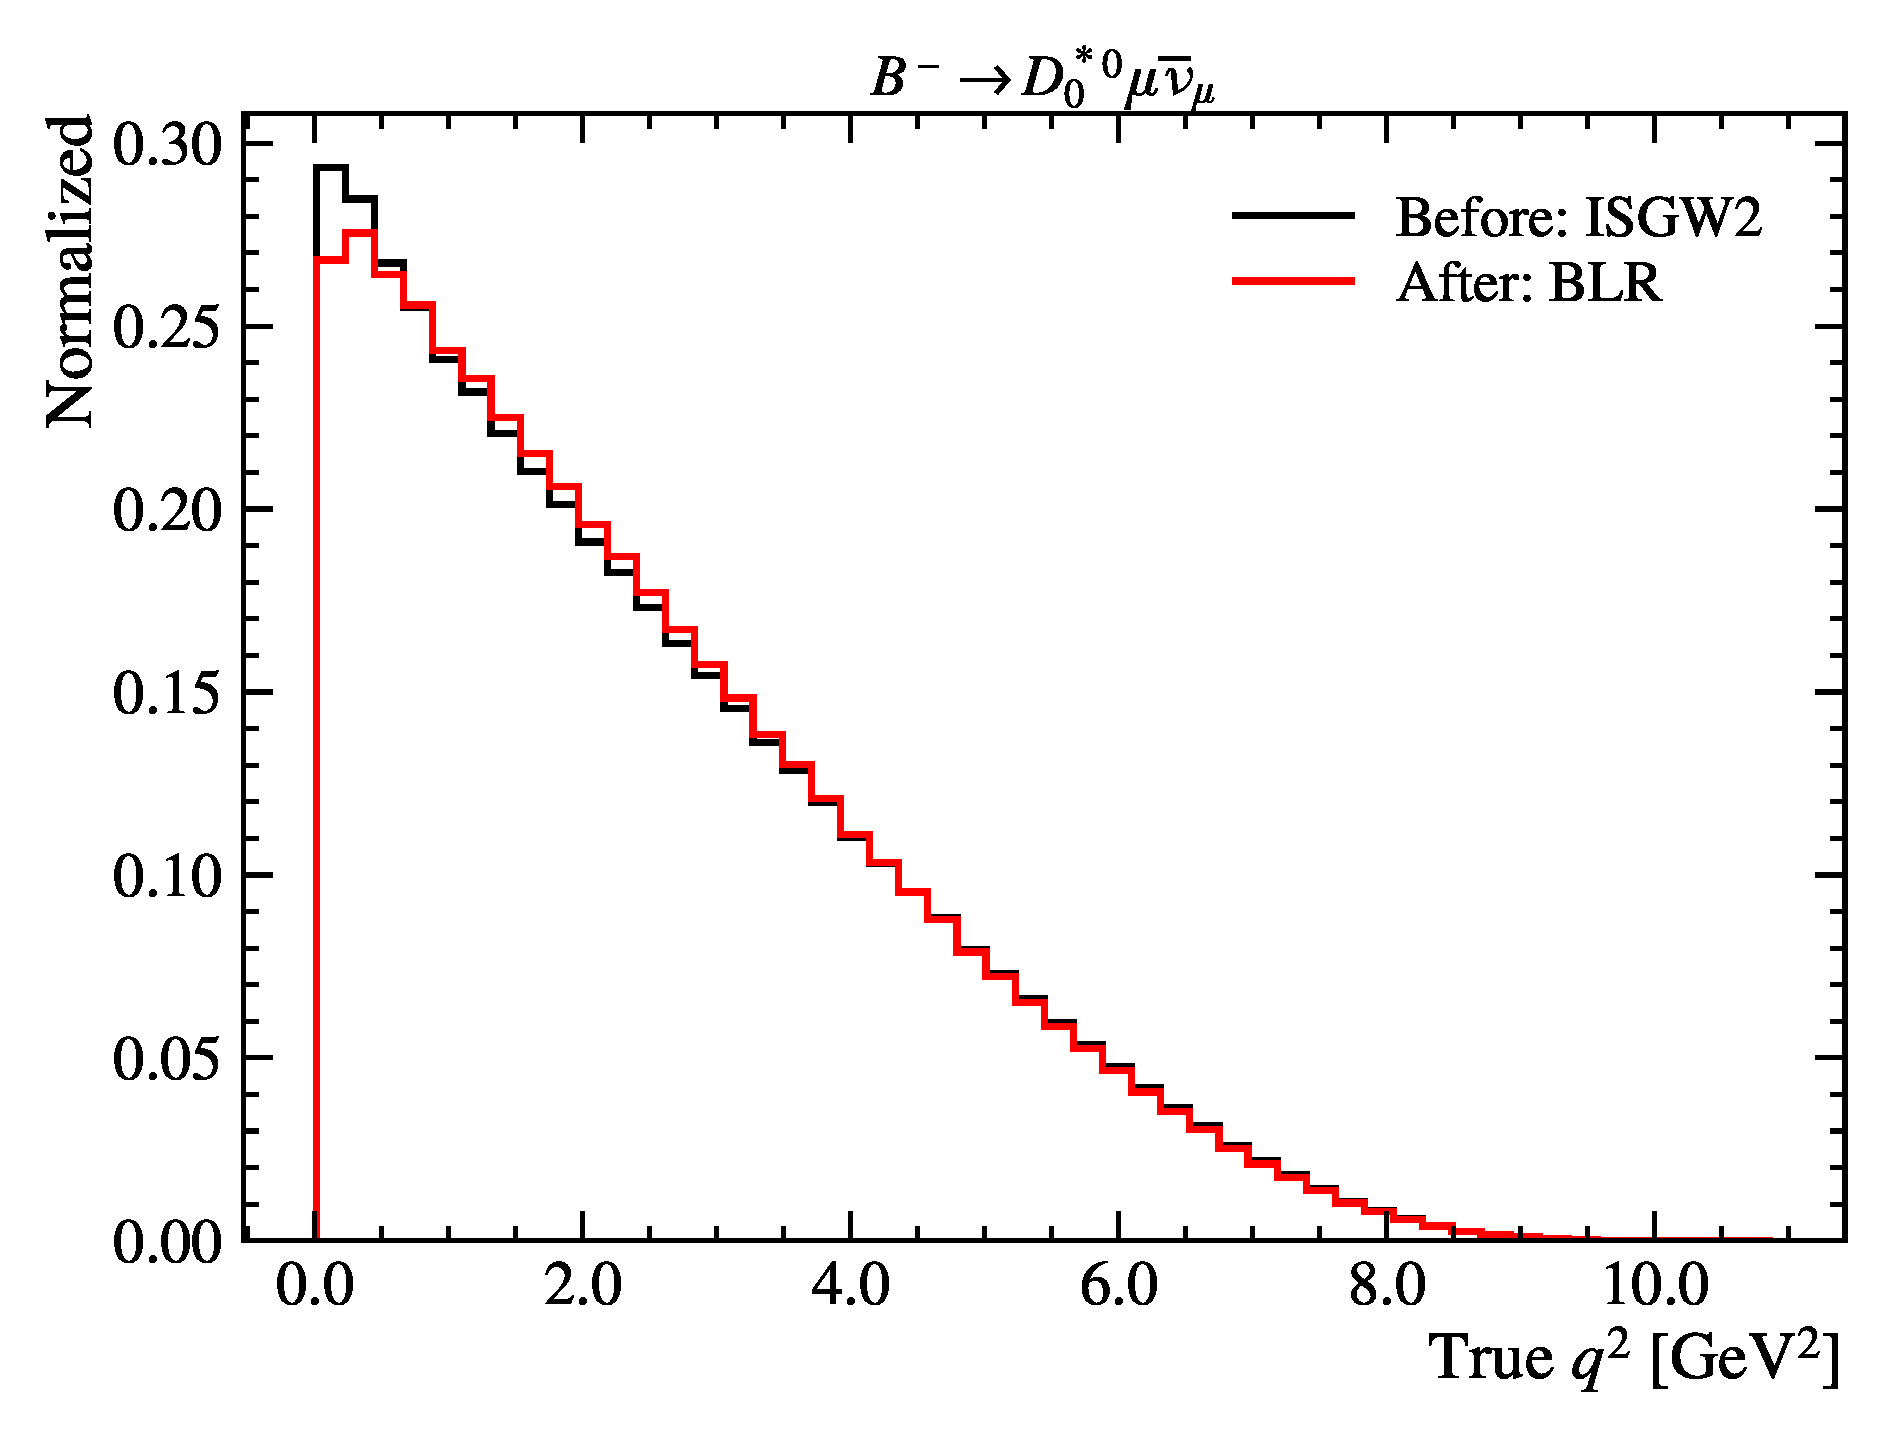
\includegraphics[width=0.24\textwidth]{
        ./figs-supplemental-plots/Dstst-form-factors/DststMu/D0stst0Mu.pdf
    }
    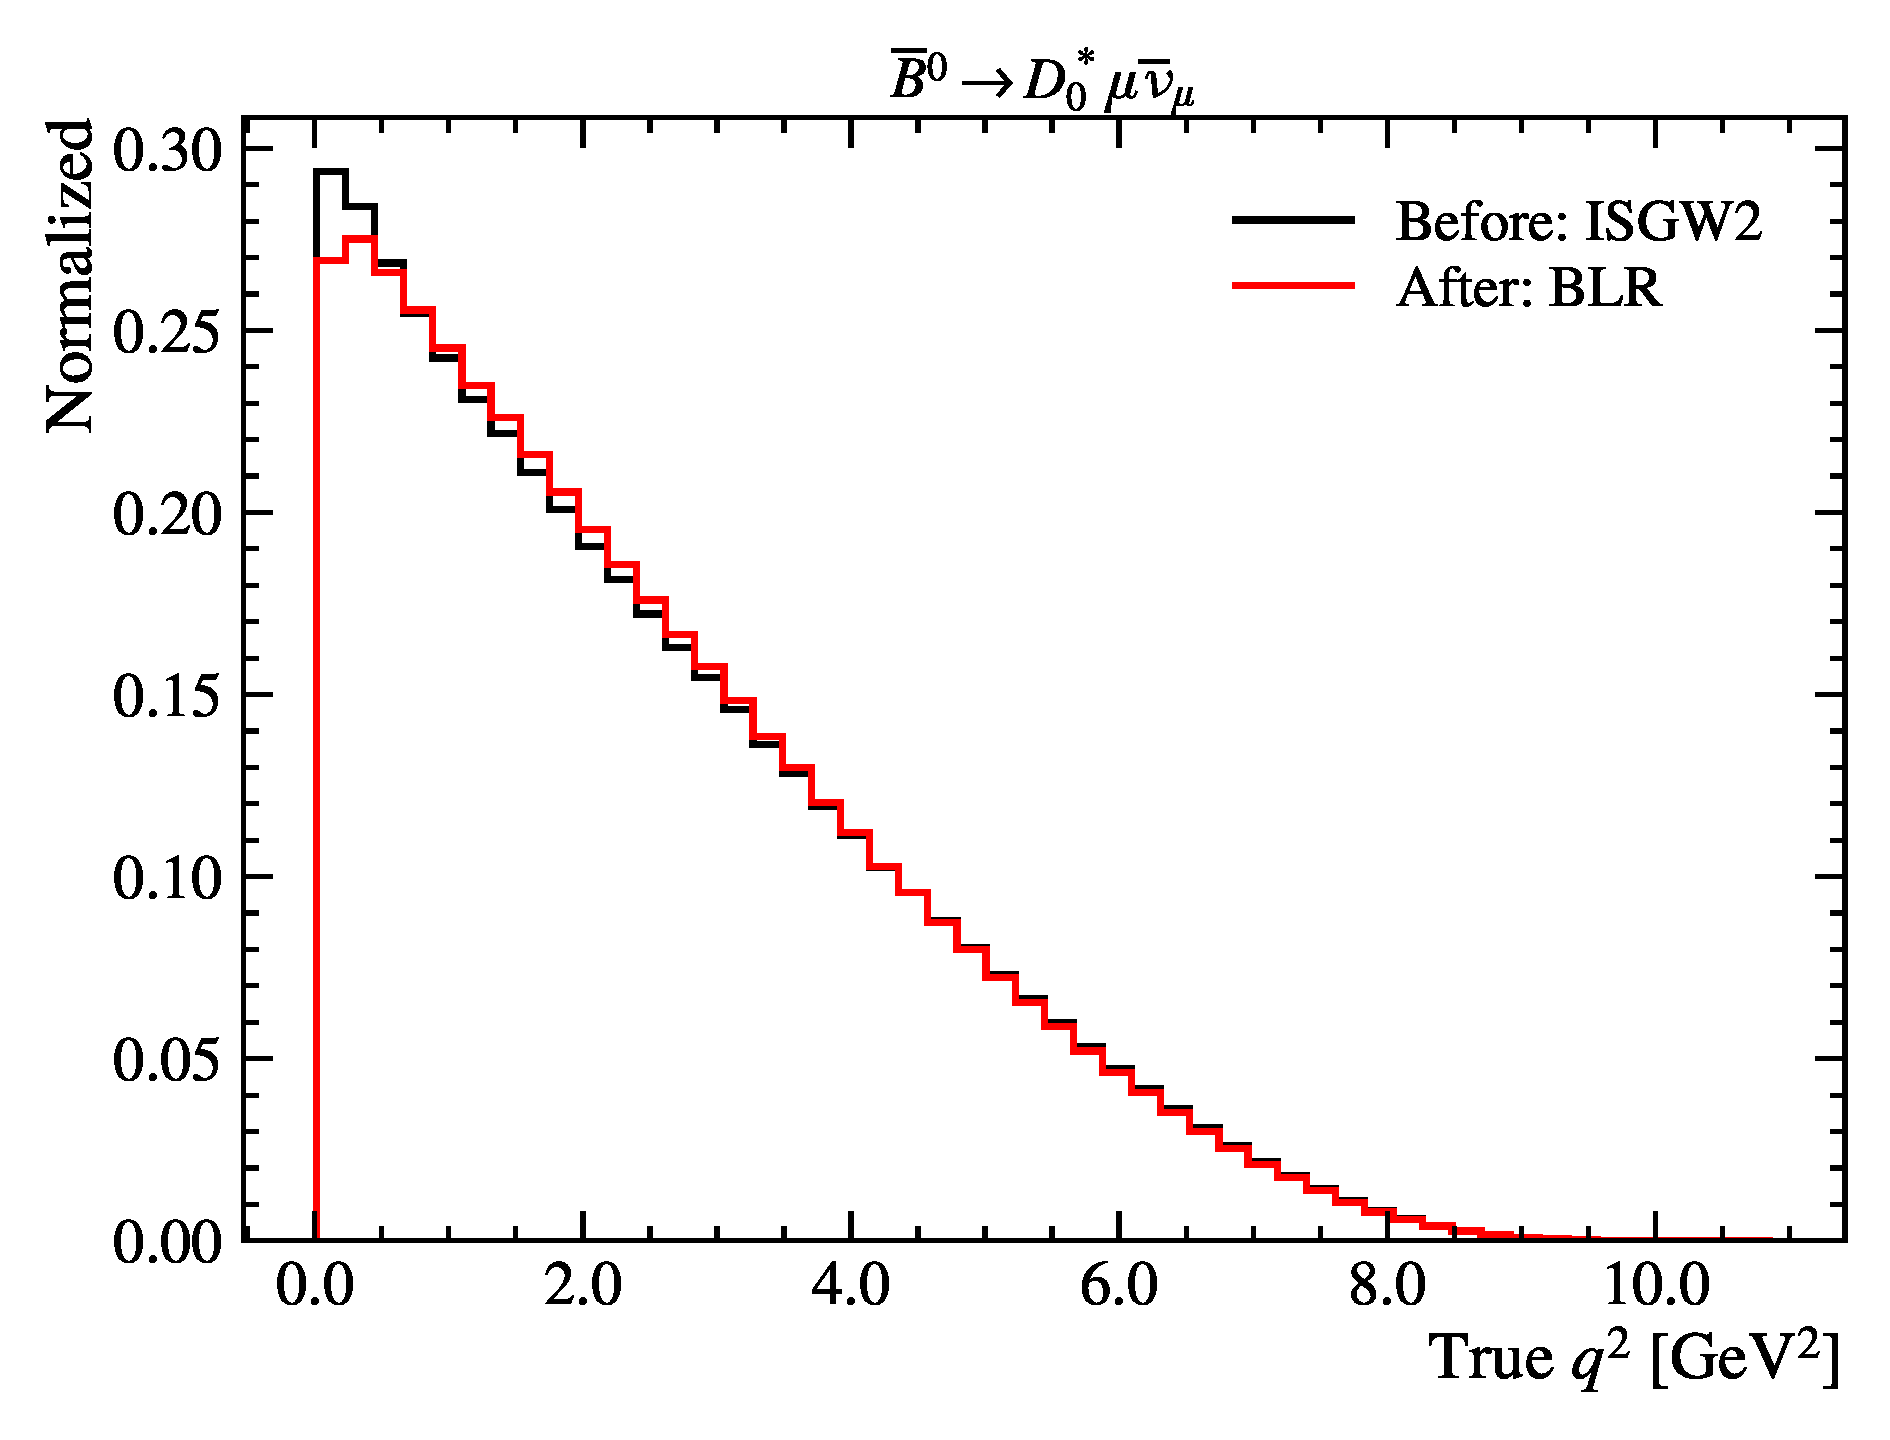
\includegraphics[width=0.24\textwidth]{
        ./figs-supplemental-plots/Dstst-form-factors/DststMu/D0ststMu.pdf
    }
    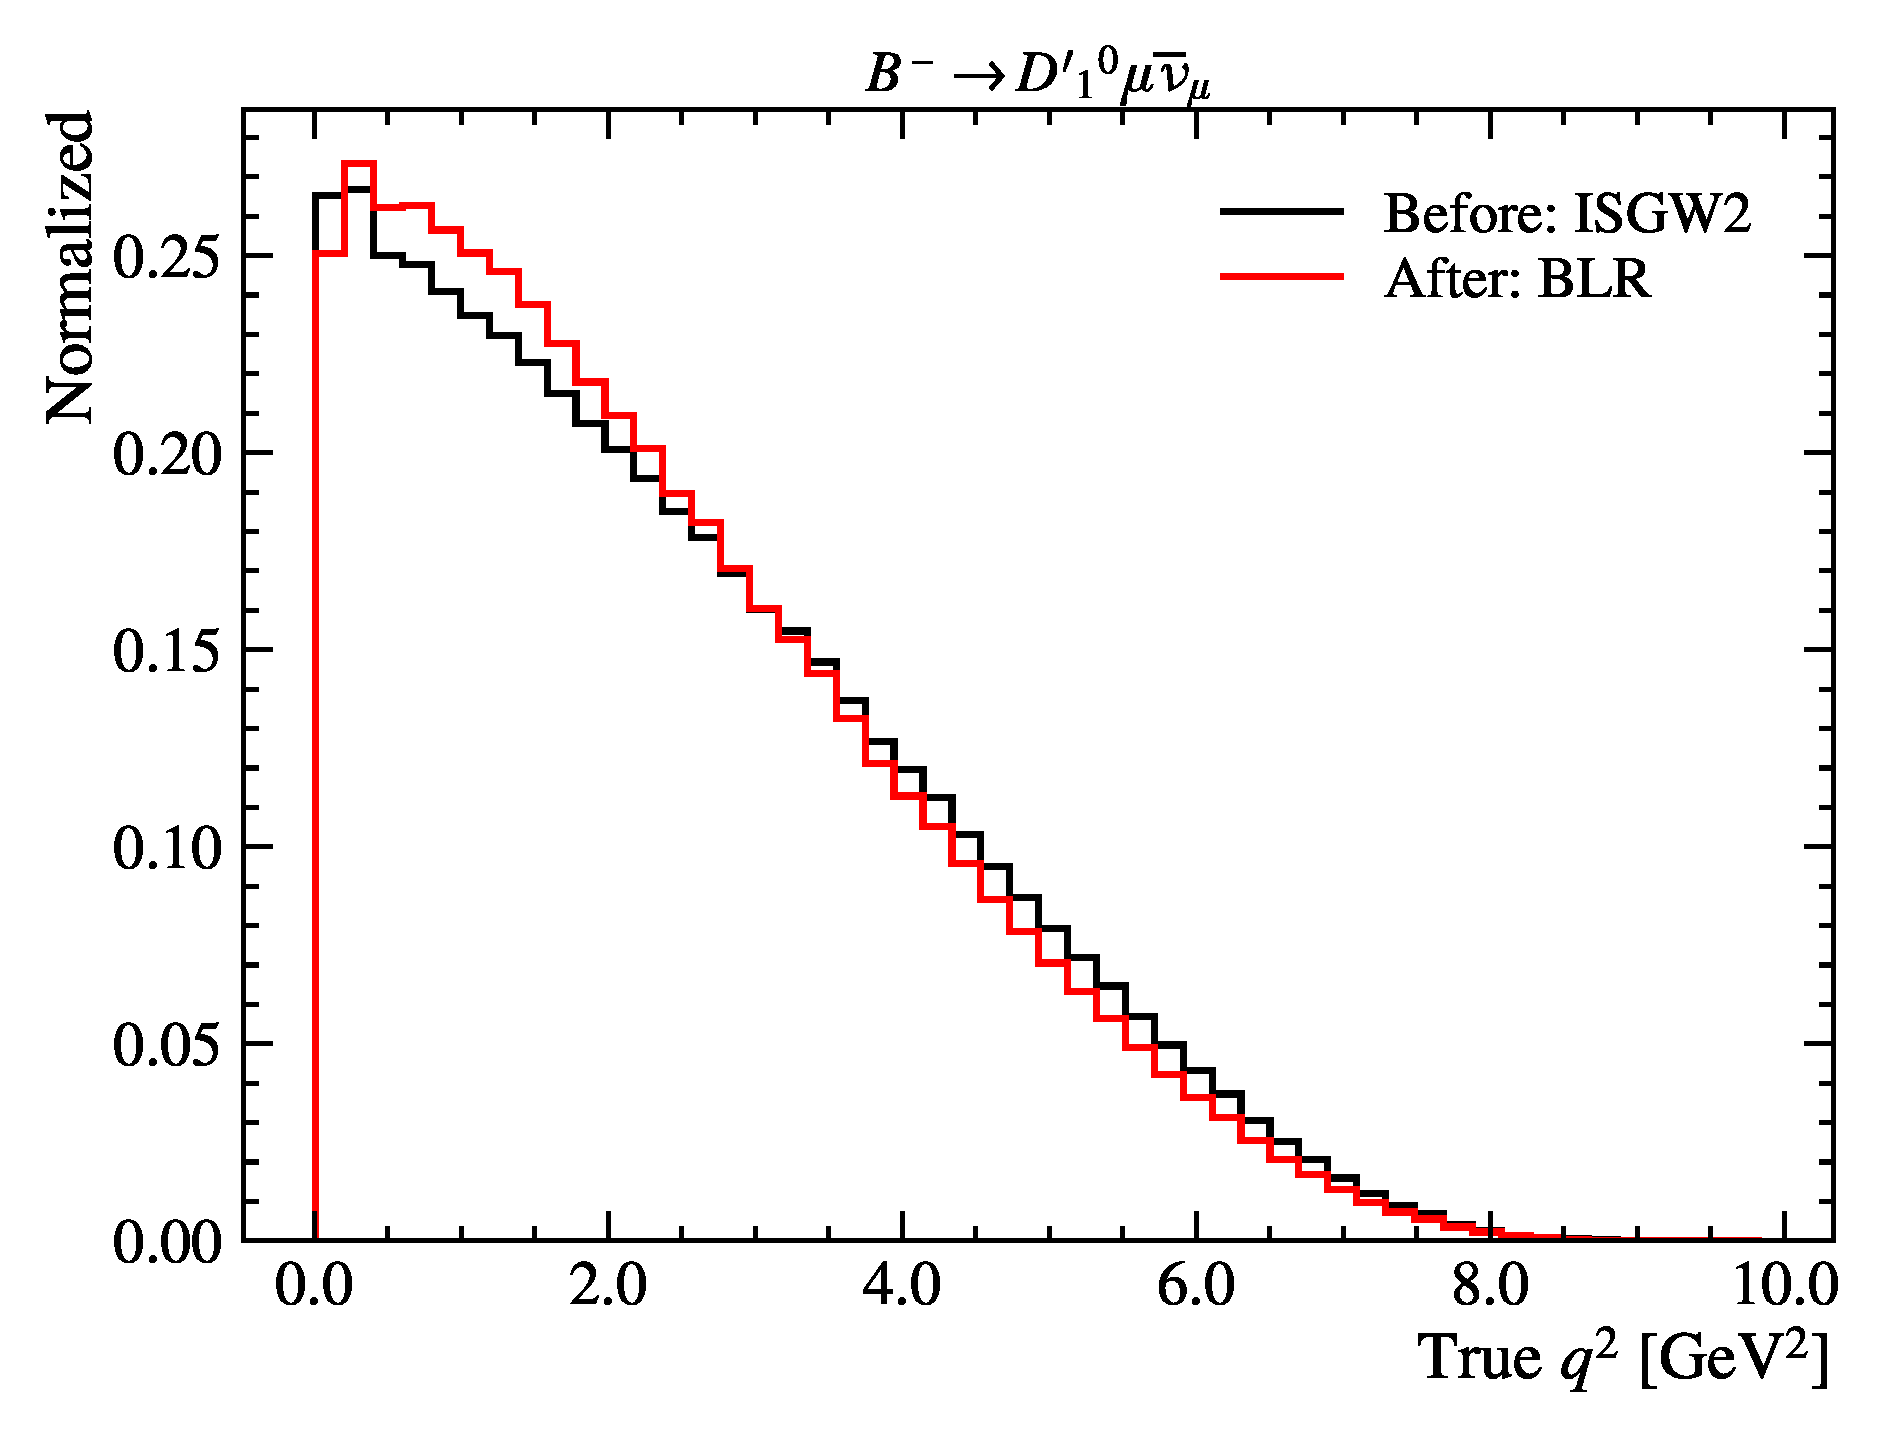
\includegraphics[width=0.24\textwidth]{
        ./figs-supplemental-plots/Dstst-form-factors/DststMu/D1pstst0Mu.pdf
    }
    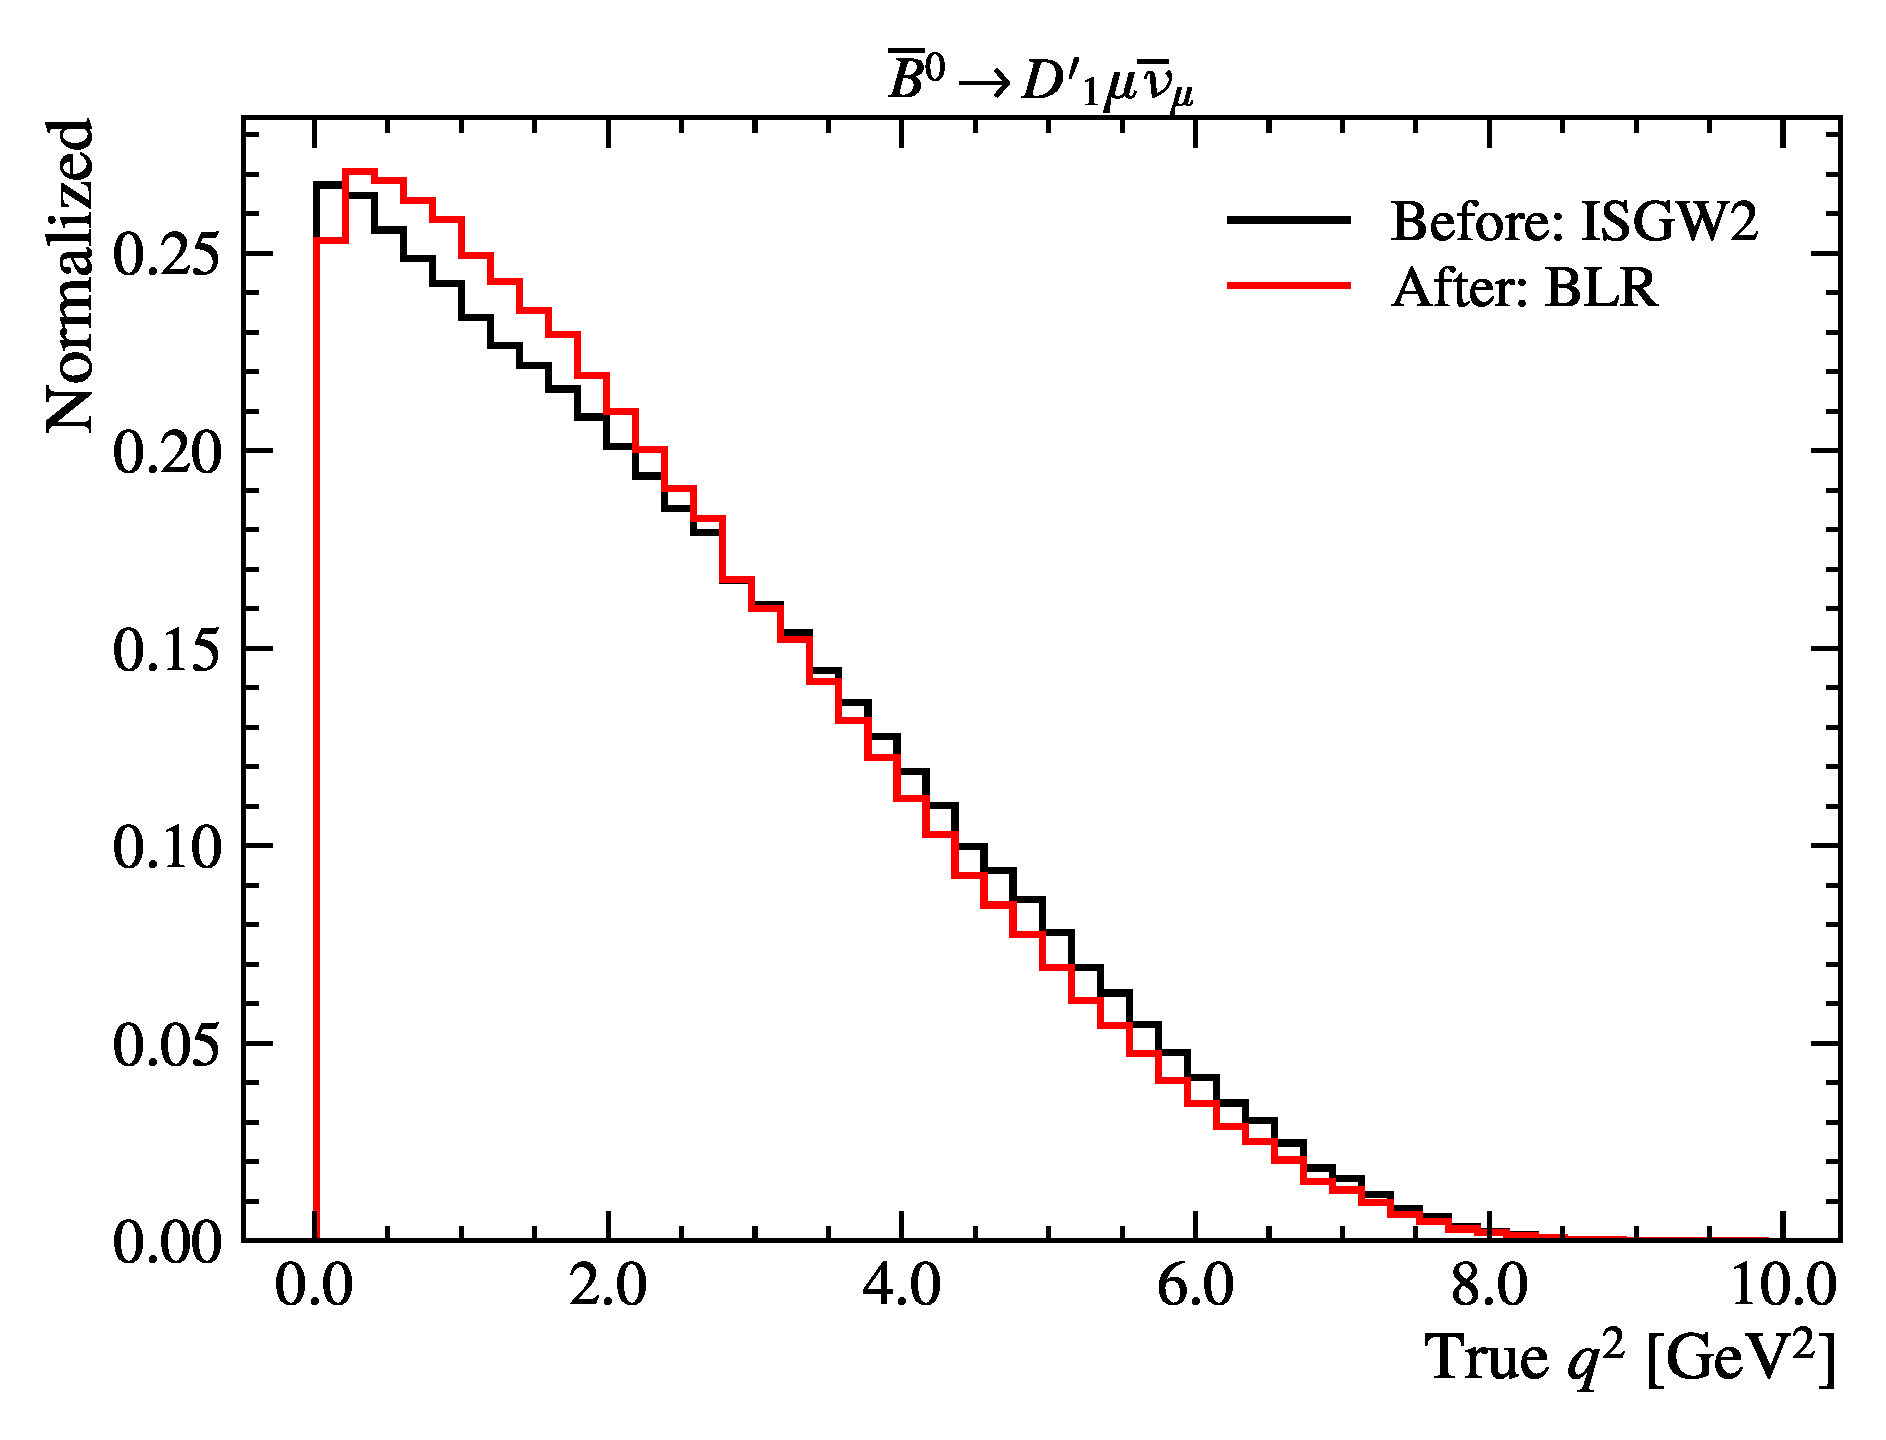
\includegraphics[width=0.24\textwidth]{
        ./figs-supplemental-plots/Dstst-form-factors/DststMu/D1pststMu.pdf
    }

    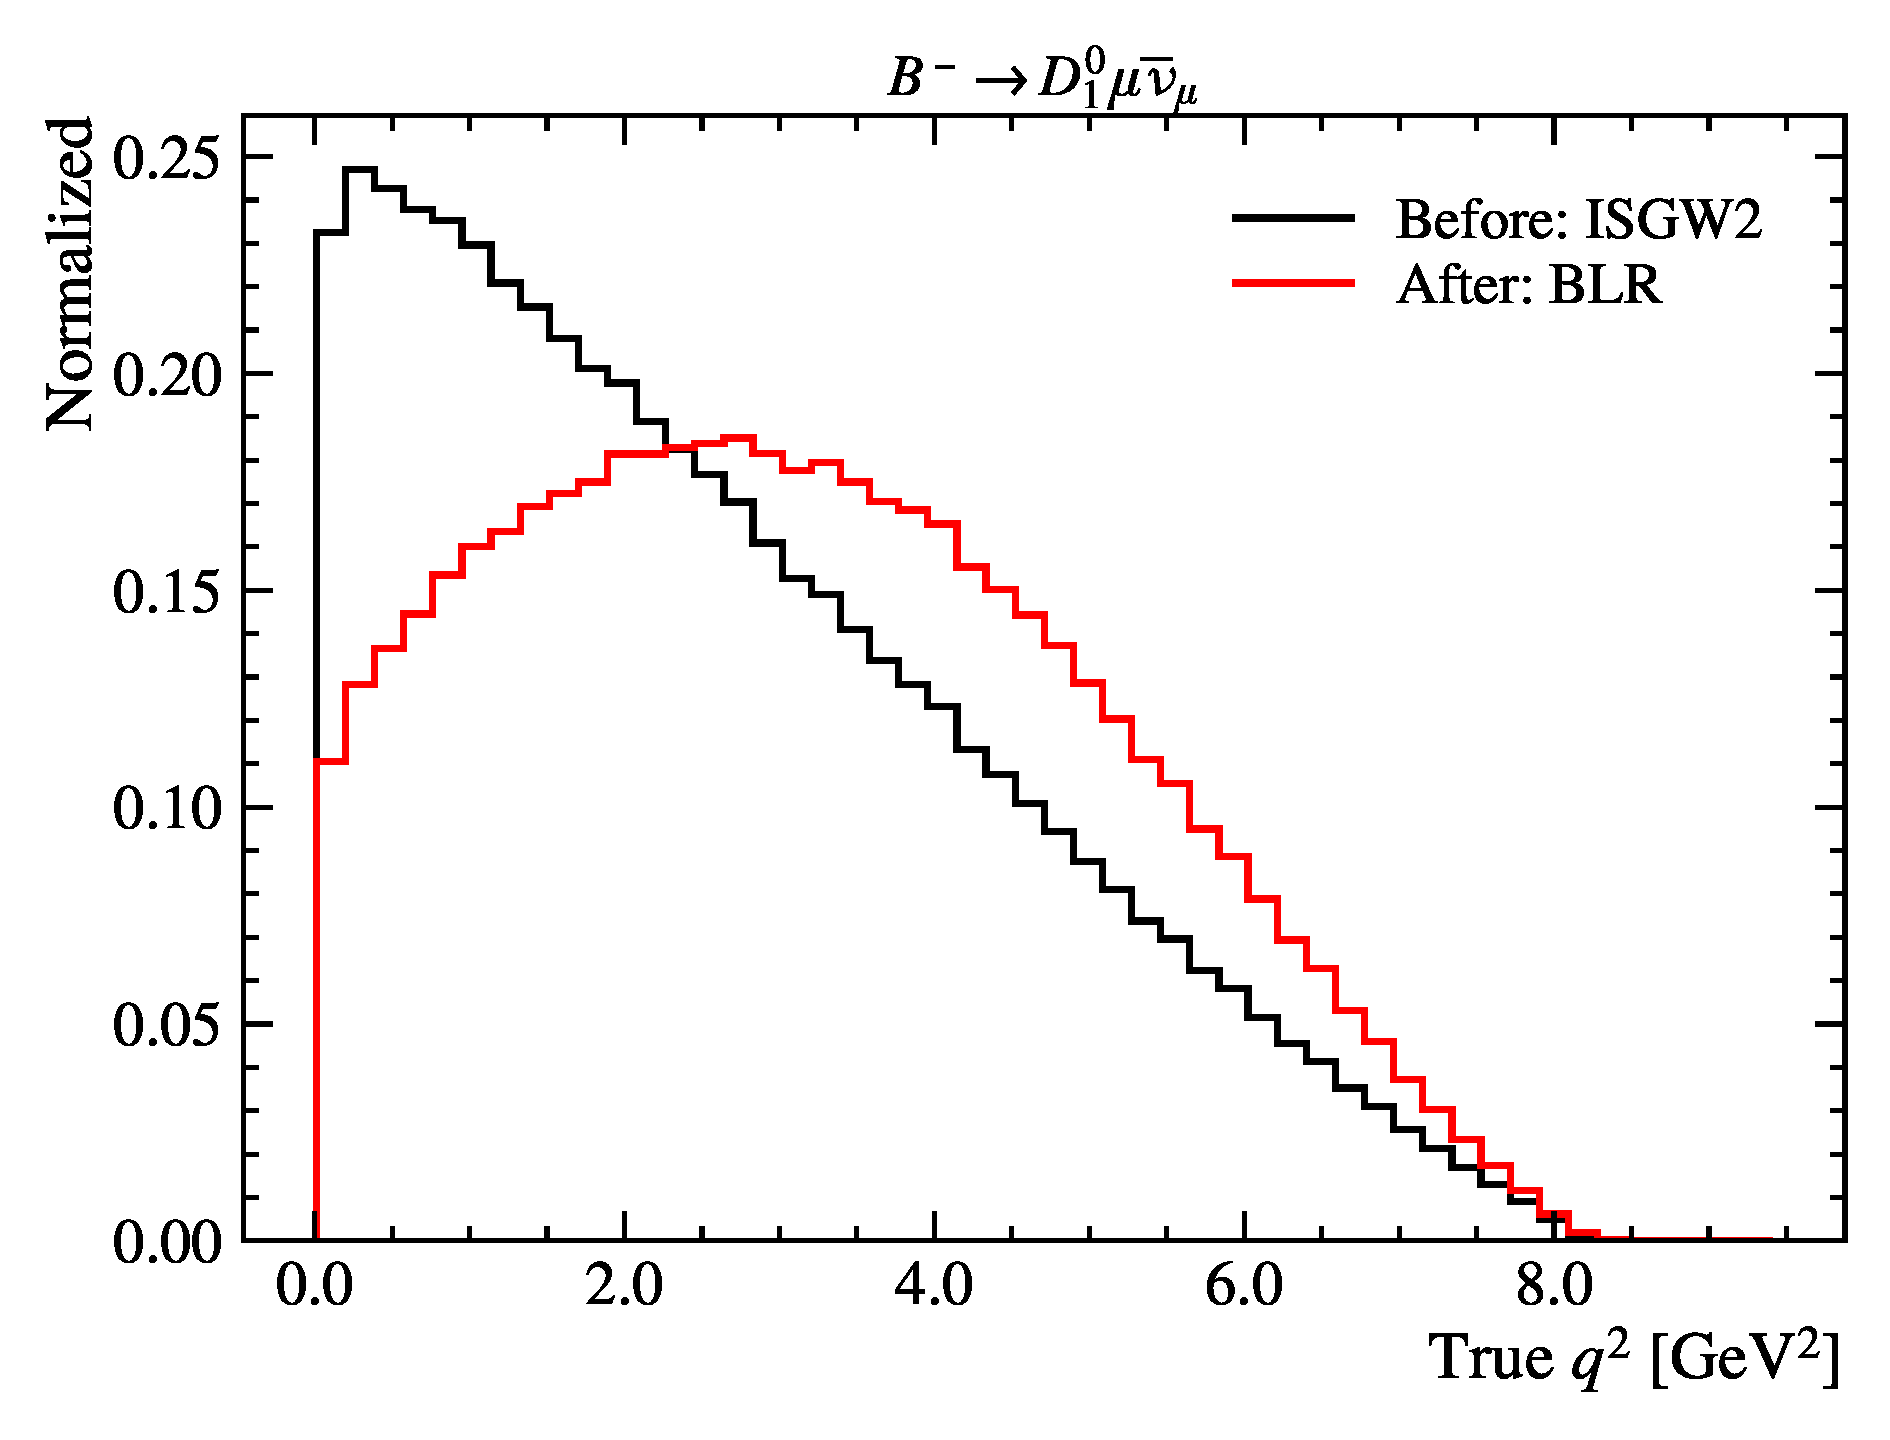
\includegraphics[width=0.24\textwidth]{
        ./figs-supplemental-plots/Dstst-form-factors/DststMu/D1stst0Mu.pdf
    }
    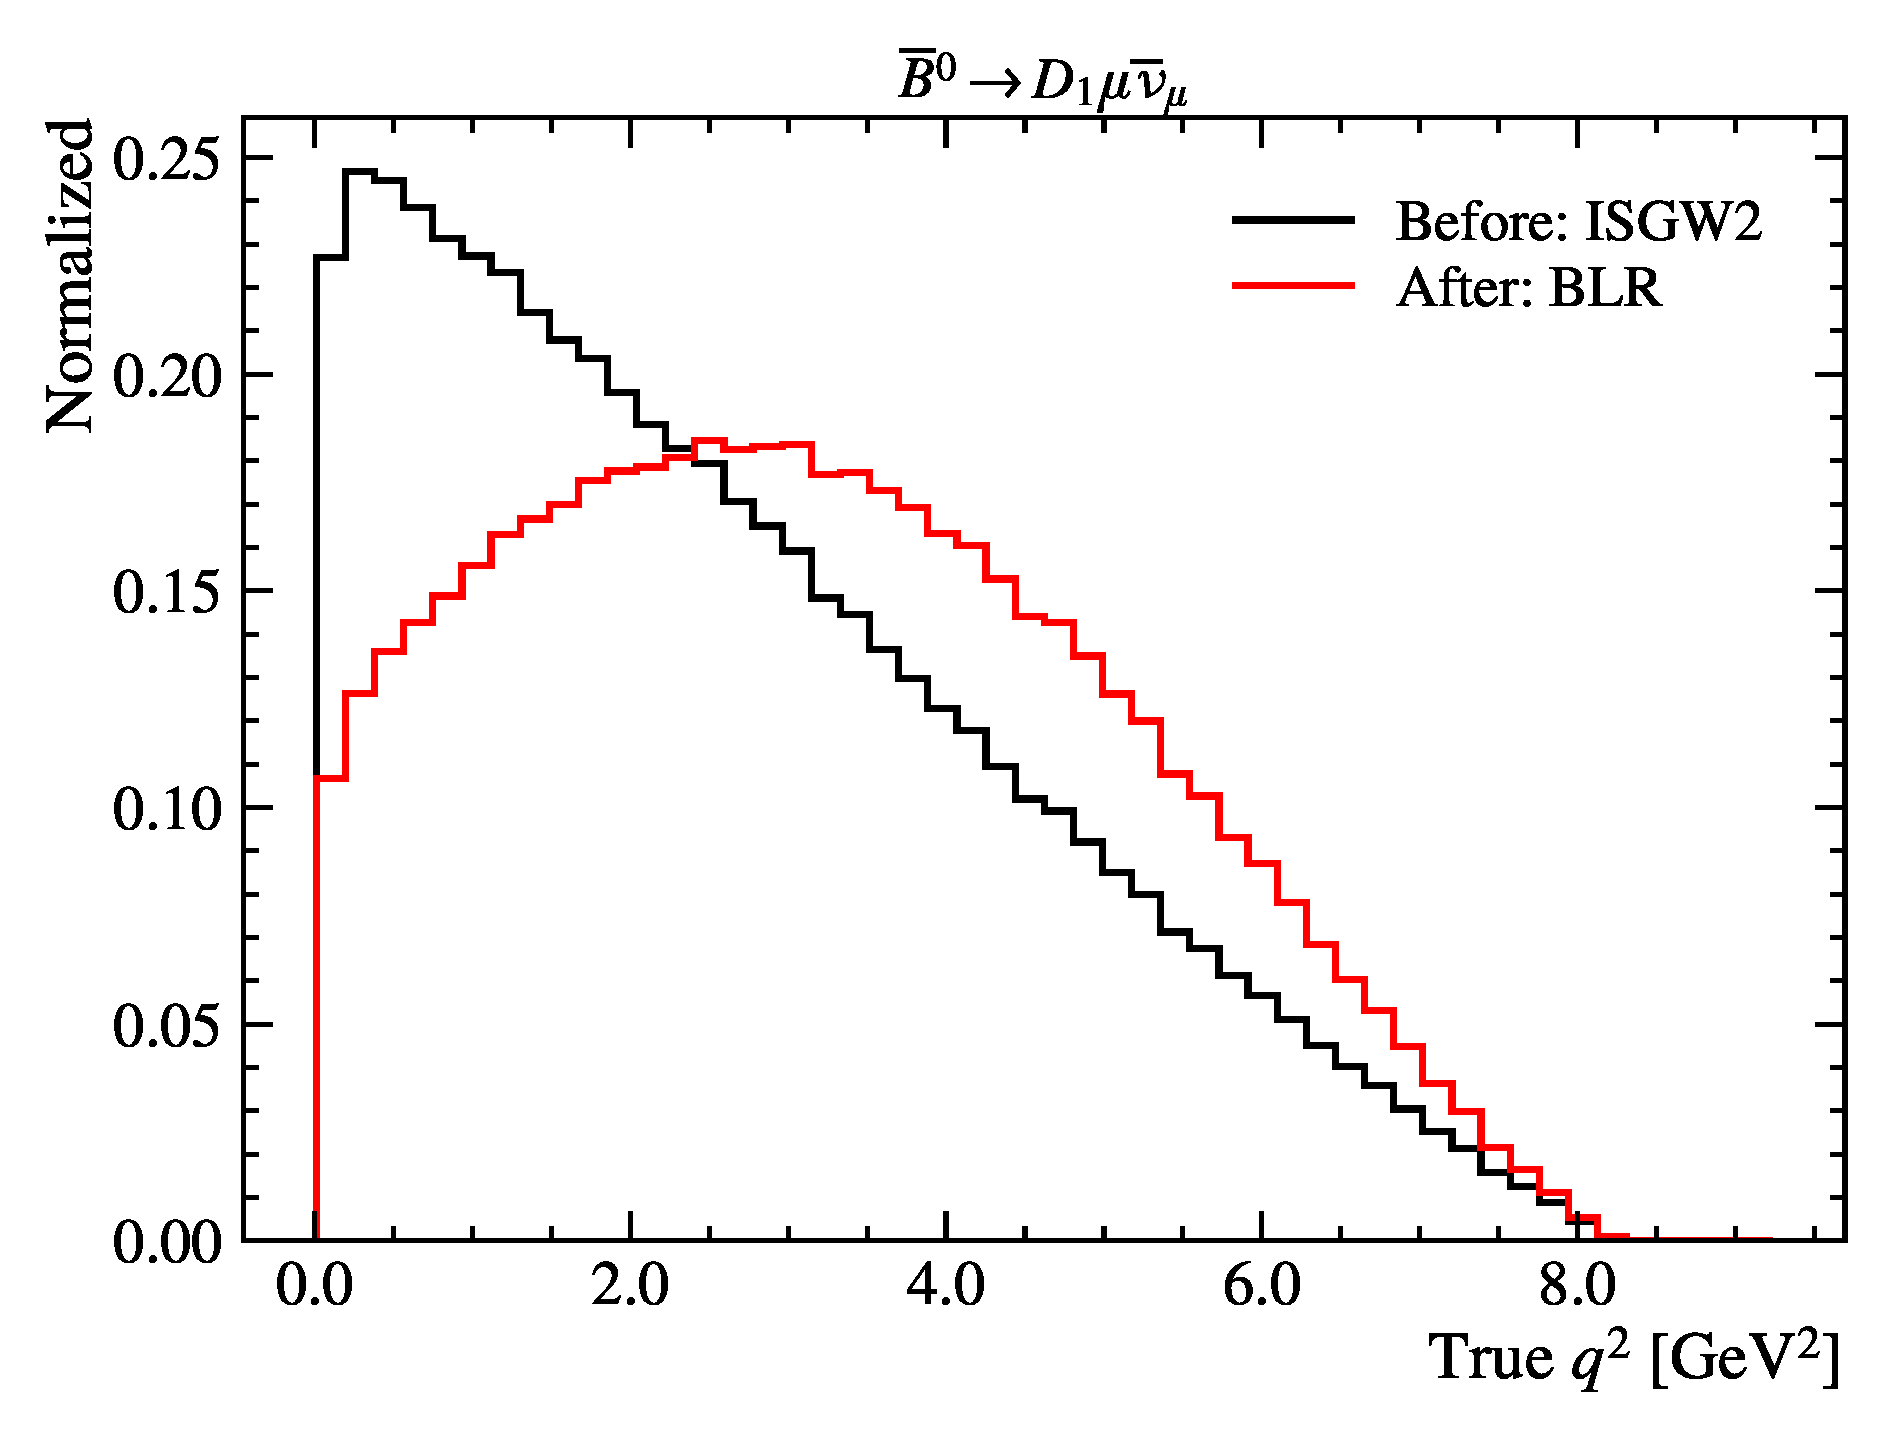
\includegraphics[width=0.24\textwidth]{
        ./figs-supplemental-plots/Dstst-form-factors/DststMu/D1ststMu.pdf
    }
    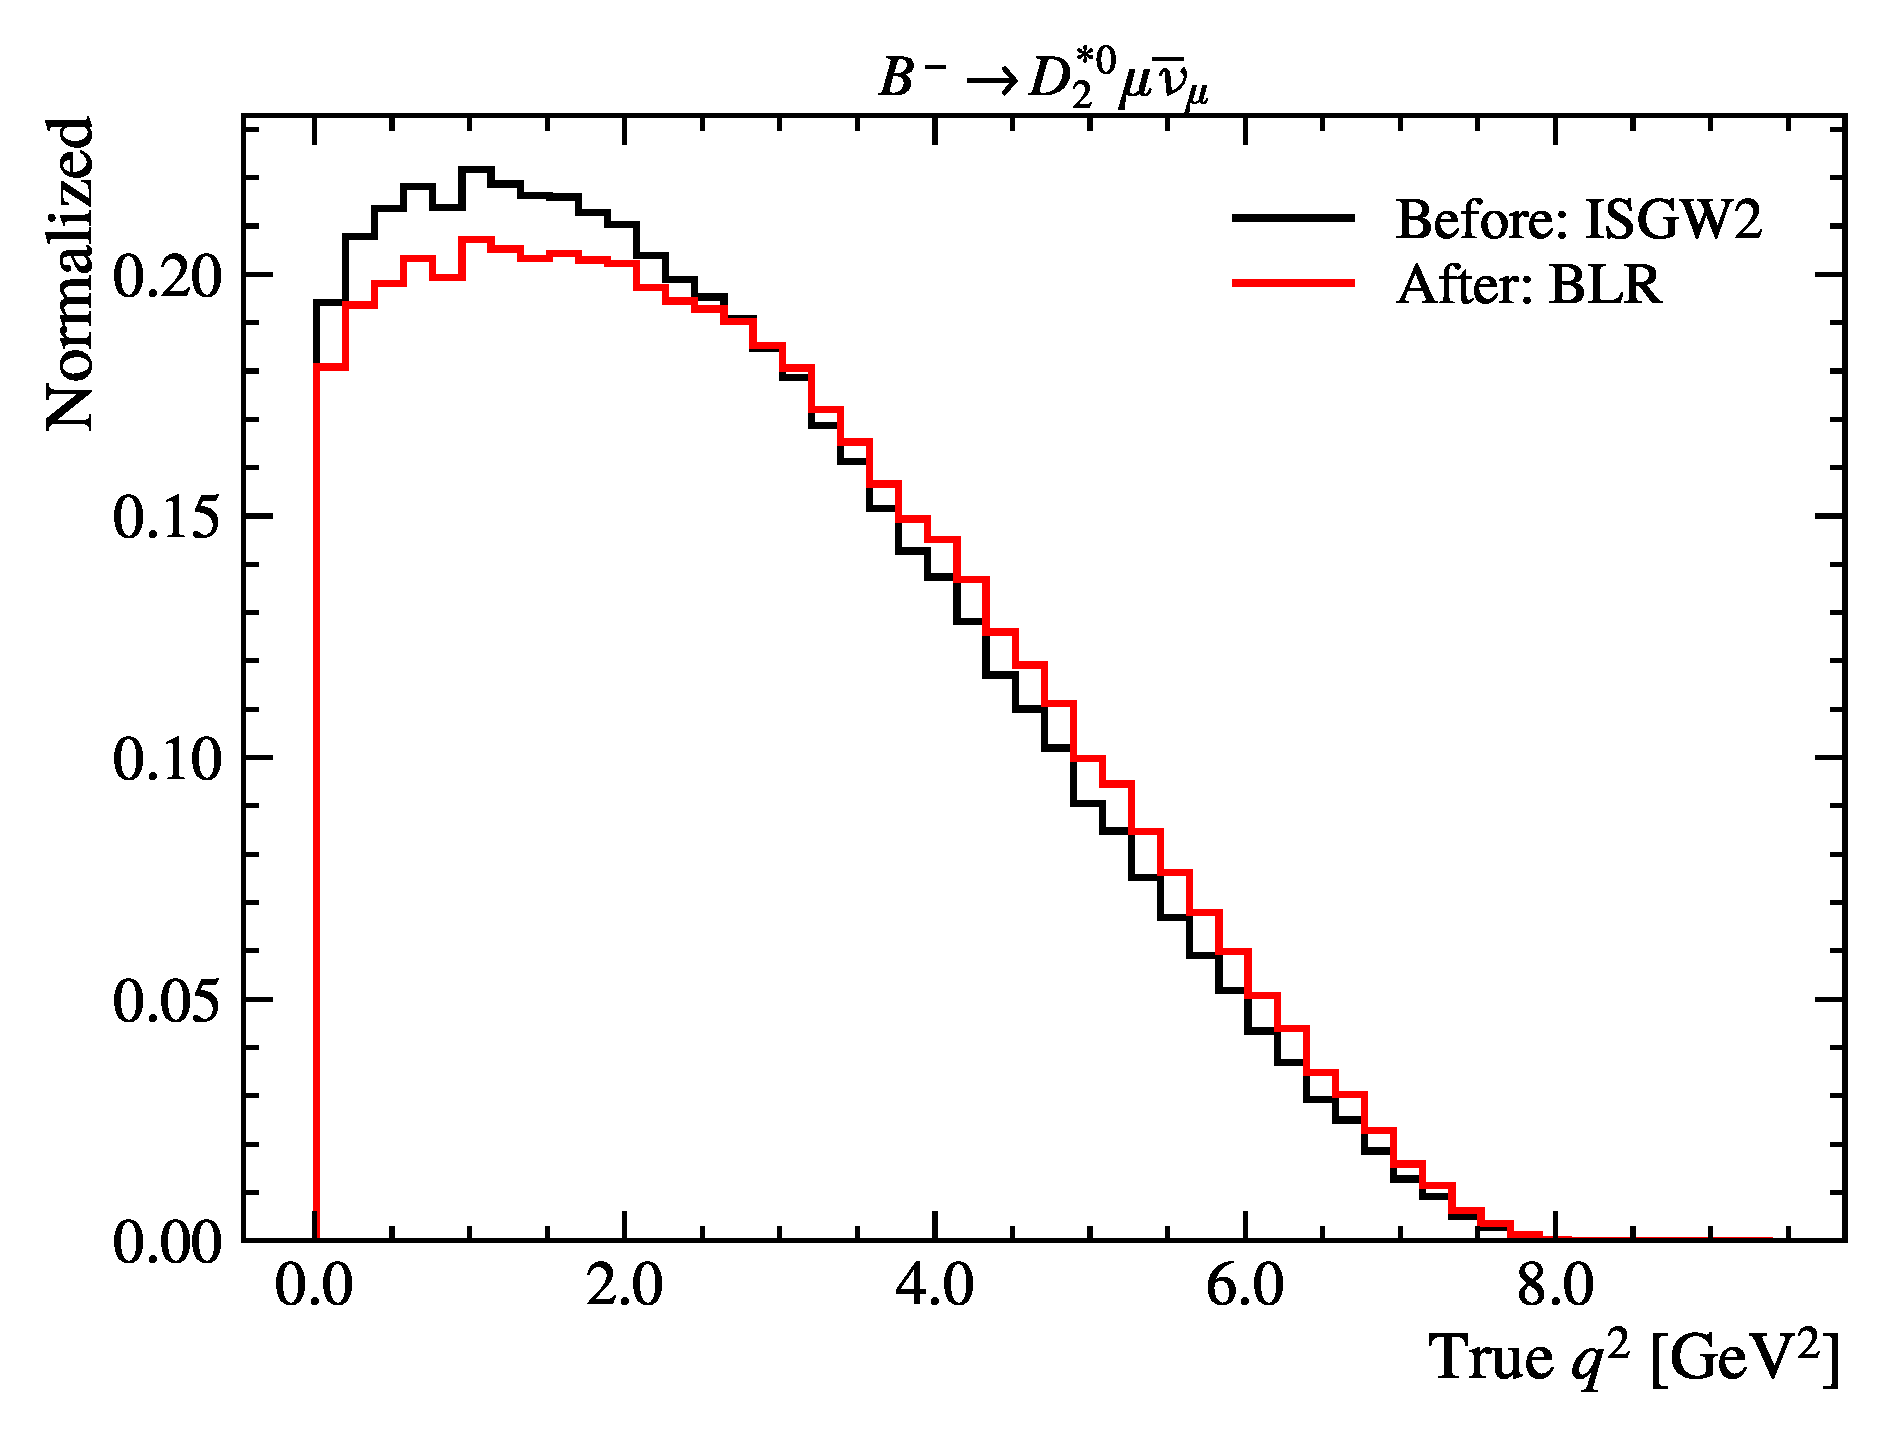
\includegraphics[width=0.24\textwidth]{
        ./figs-supplemental-plots/Dstst-form-factors/DststMu/D2stst0Mu.pdf
    }
    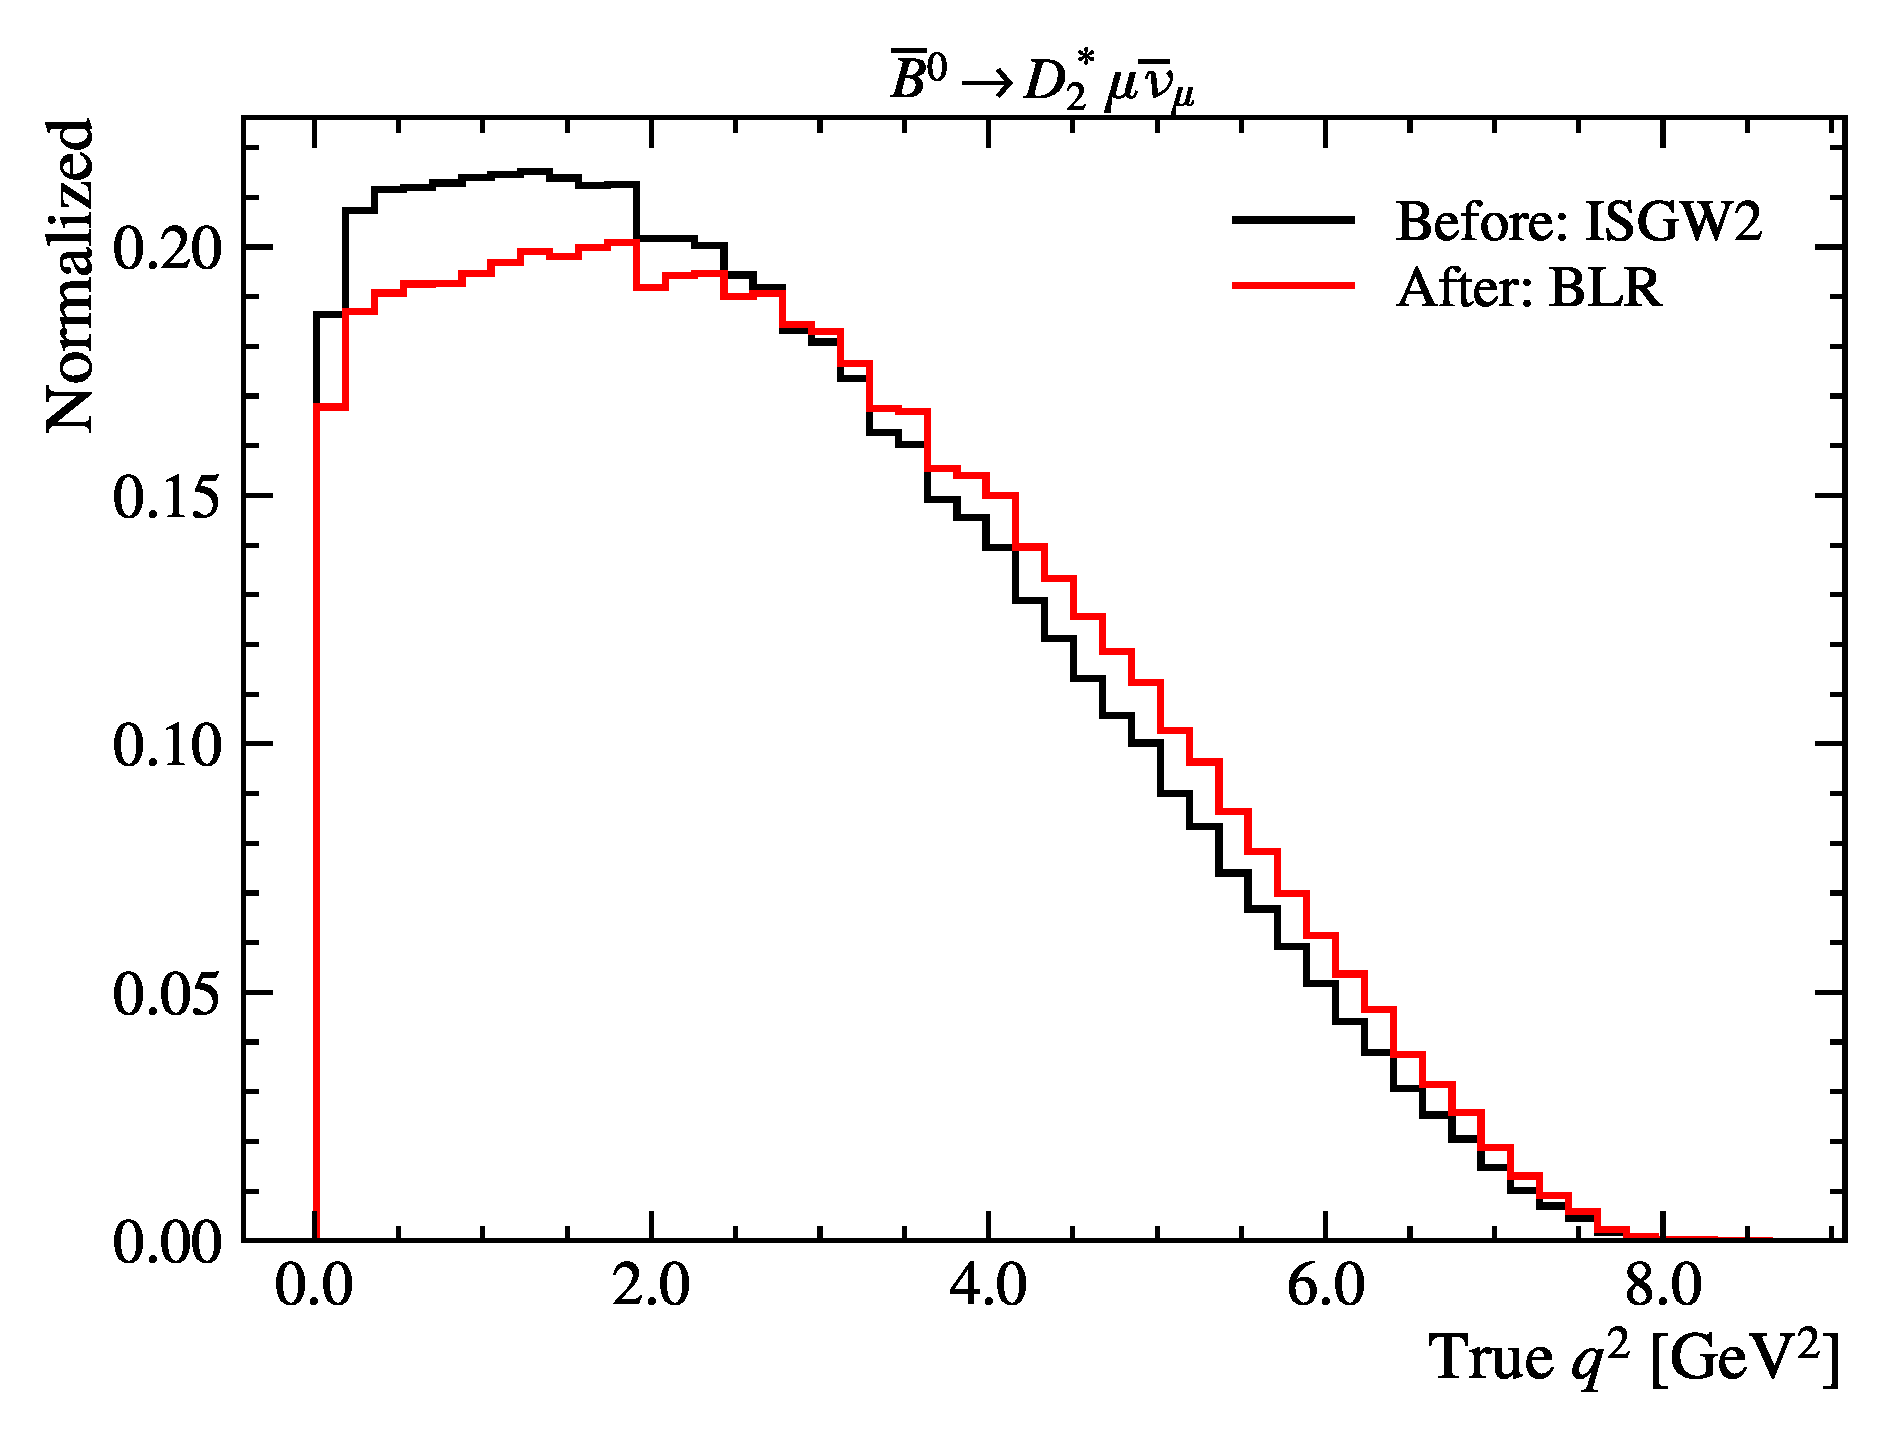
\includegraphics[width=0.24\textwidth]{
        ./figs-supplemental-plots/Dstst-form-factors/DststMu/D2ststMu.pdf
    }

    \caption{
        Form factor reweight effect on $D^{**}\mu$ MC templates.
        Parameters are taken verbatim from \cite{Bernlochner_2018}.
    }
    \label{fig:ff-rwt-raw-Dstst-norm-like}
\end{figure}

\begin{figure}[ht]
    \centering
    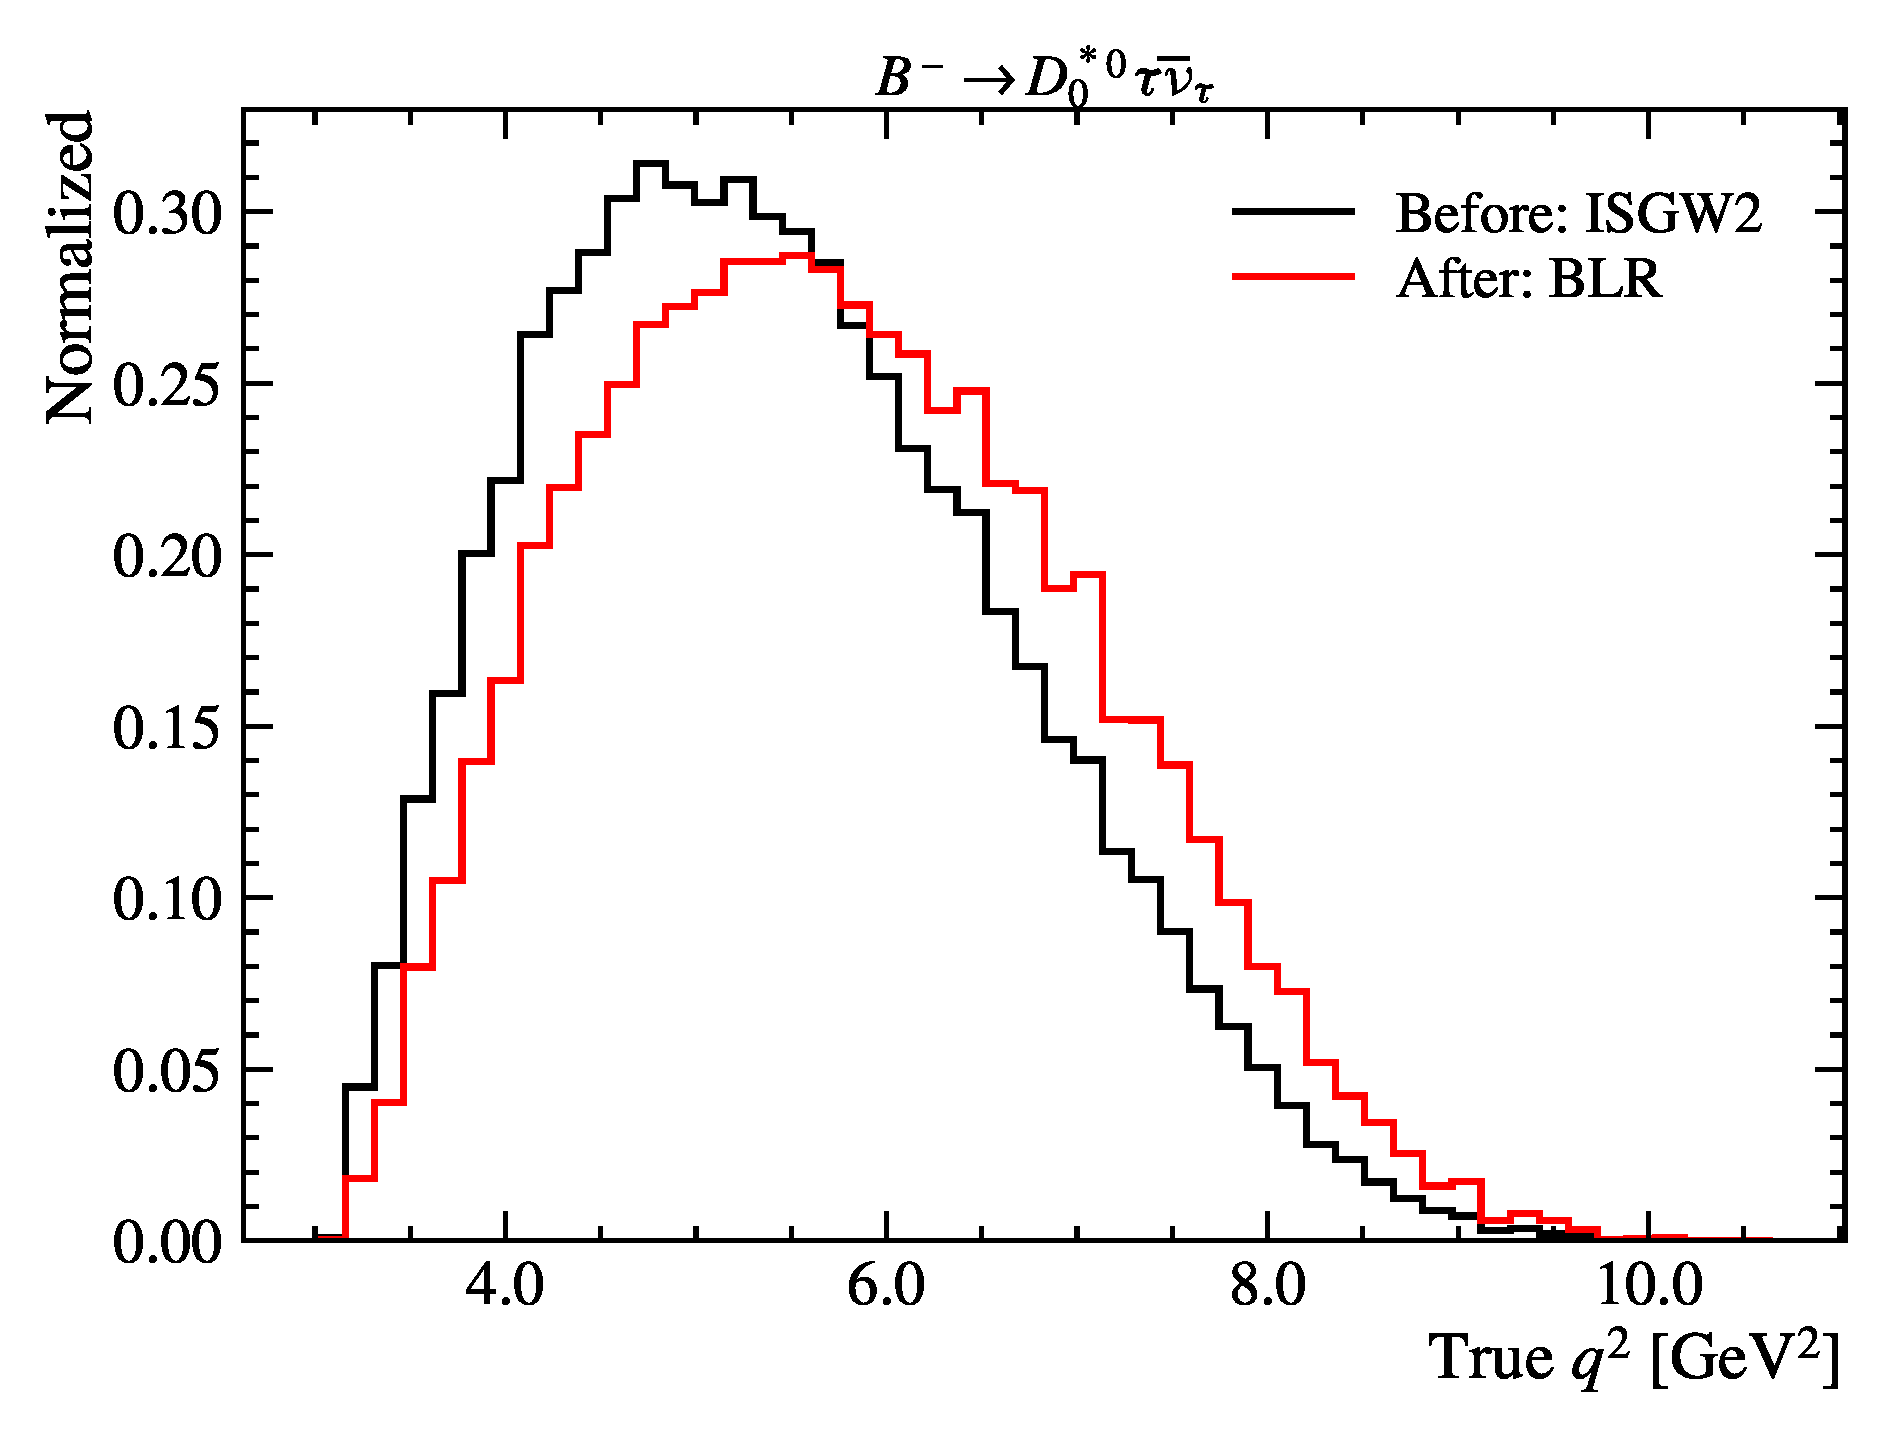
\includegraphics[width=0.24\textwidth]{
        ./figs-supplemental-plots/Dstst-form-factors/DststTau/D0stst0Tau.pdf
    }
    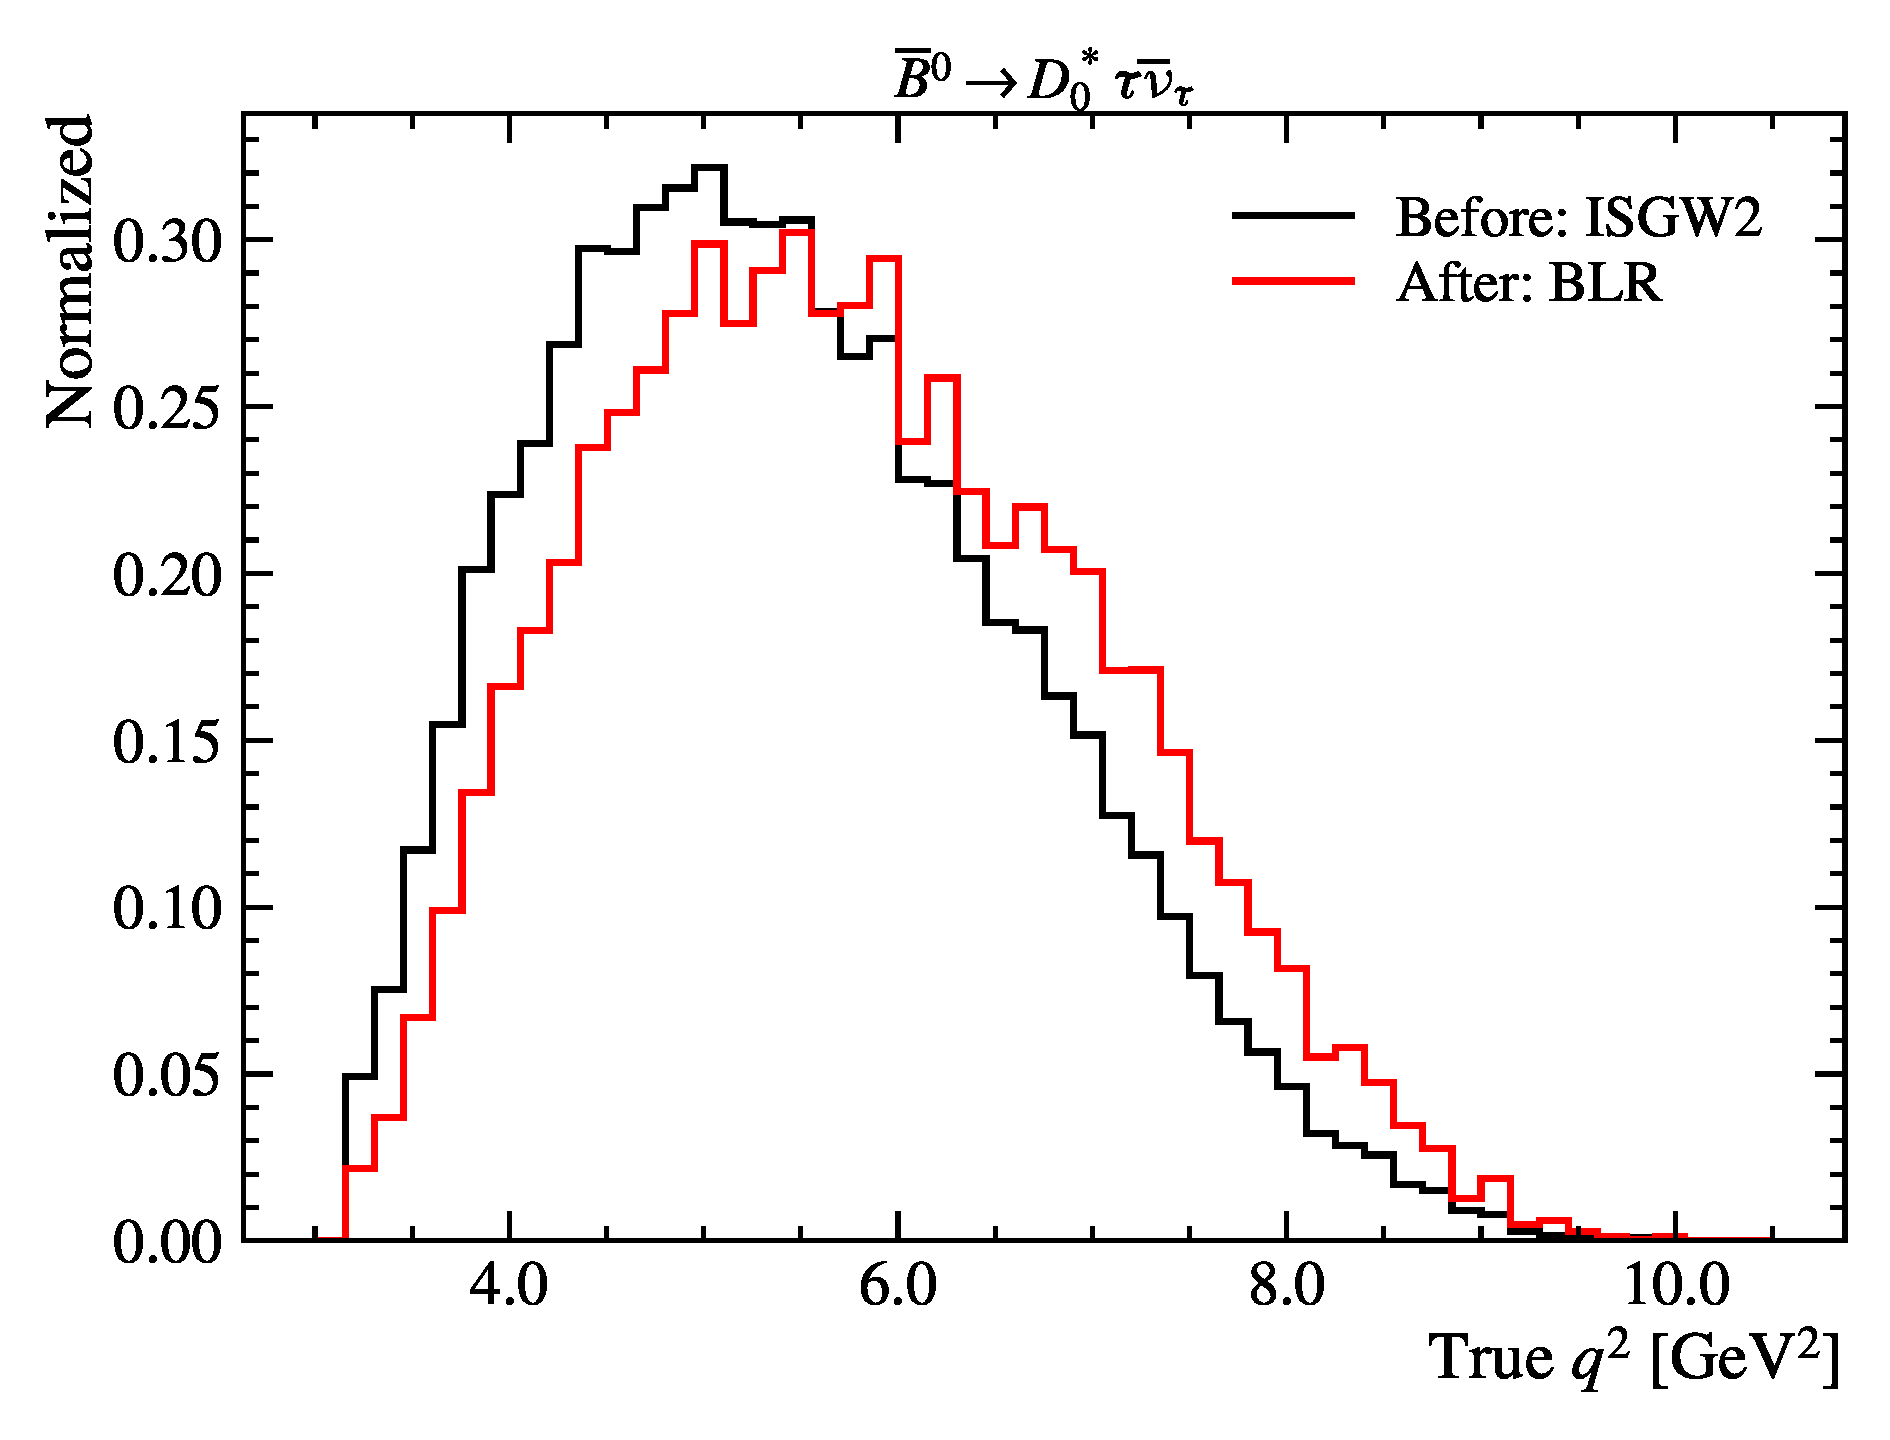
\includegraphics[width=0.24\textwidth]{
        ./figs-supplemental-plots/Dstst-form-factors/DststTau/D0ststTau.pdf
    }
    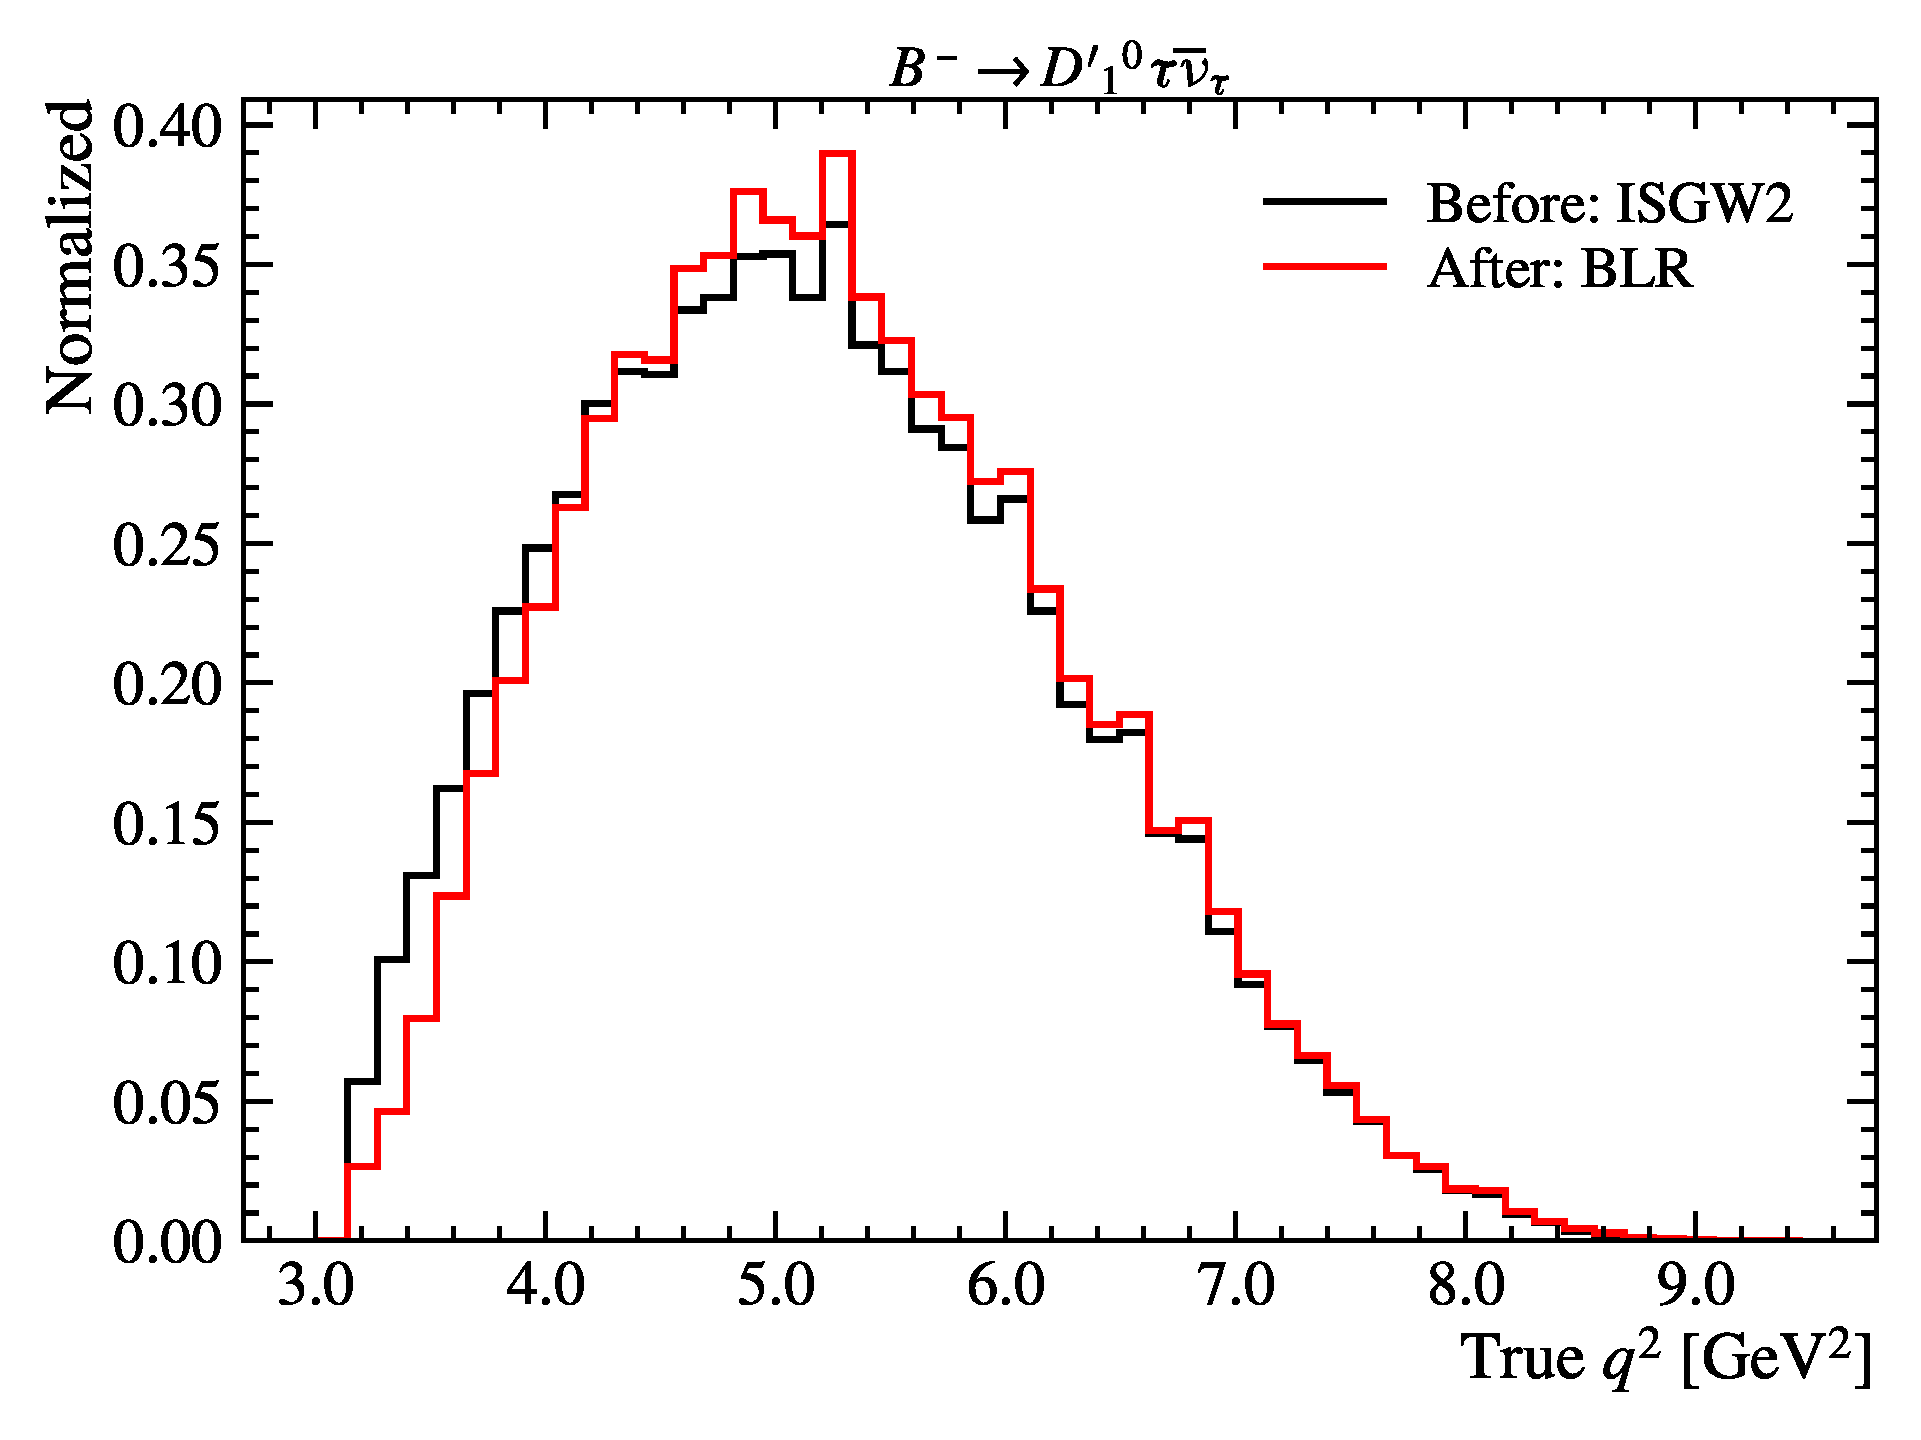
\includegraphics[width=0.24\textwidth]{
        ./figs-supplemental-plots/Dstst-form-factors/DststTau/D1pstst0Tau.pdf
    }
    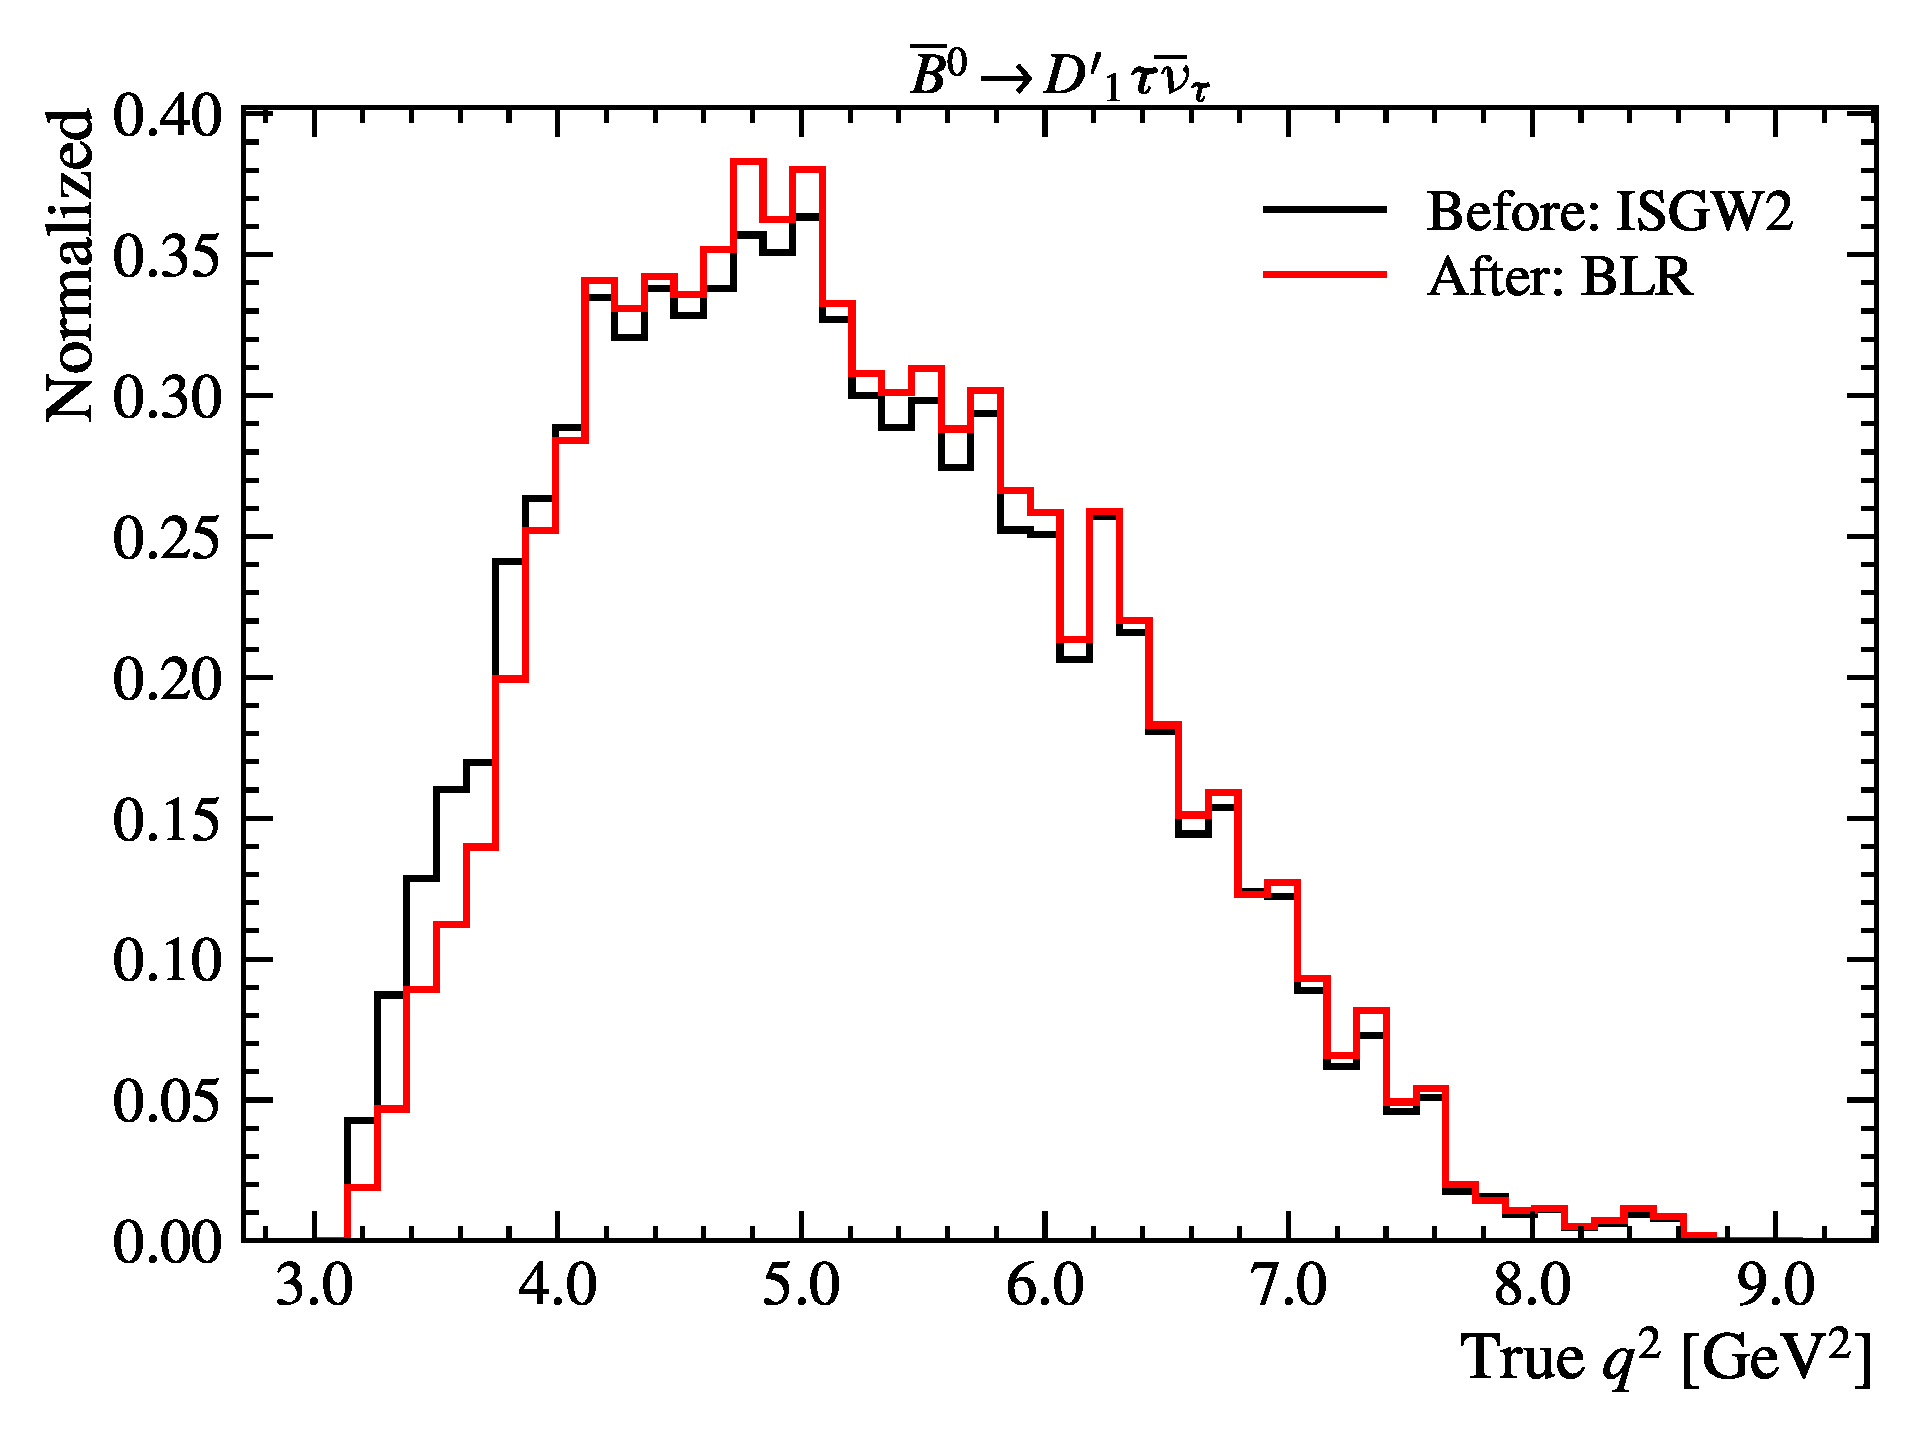
\includegraphics[width=0.24\textwidth]{
        ./figs-supplemental-plots/Dstst-form-factors/DststTau/D1pststTau.pdf
    }

    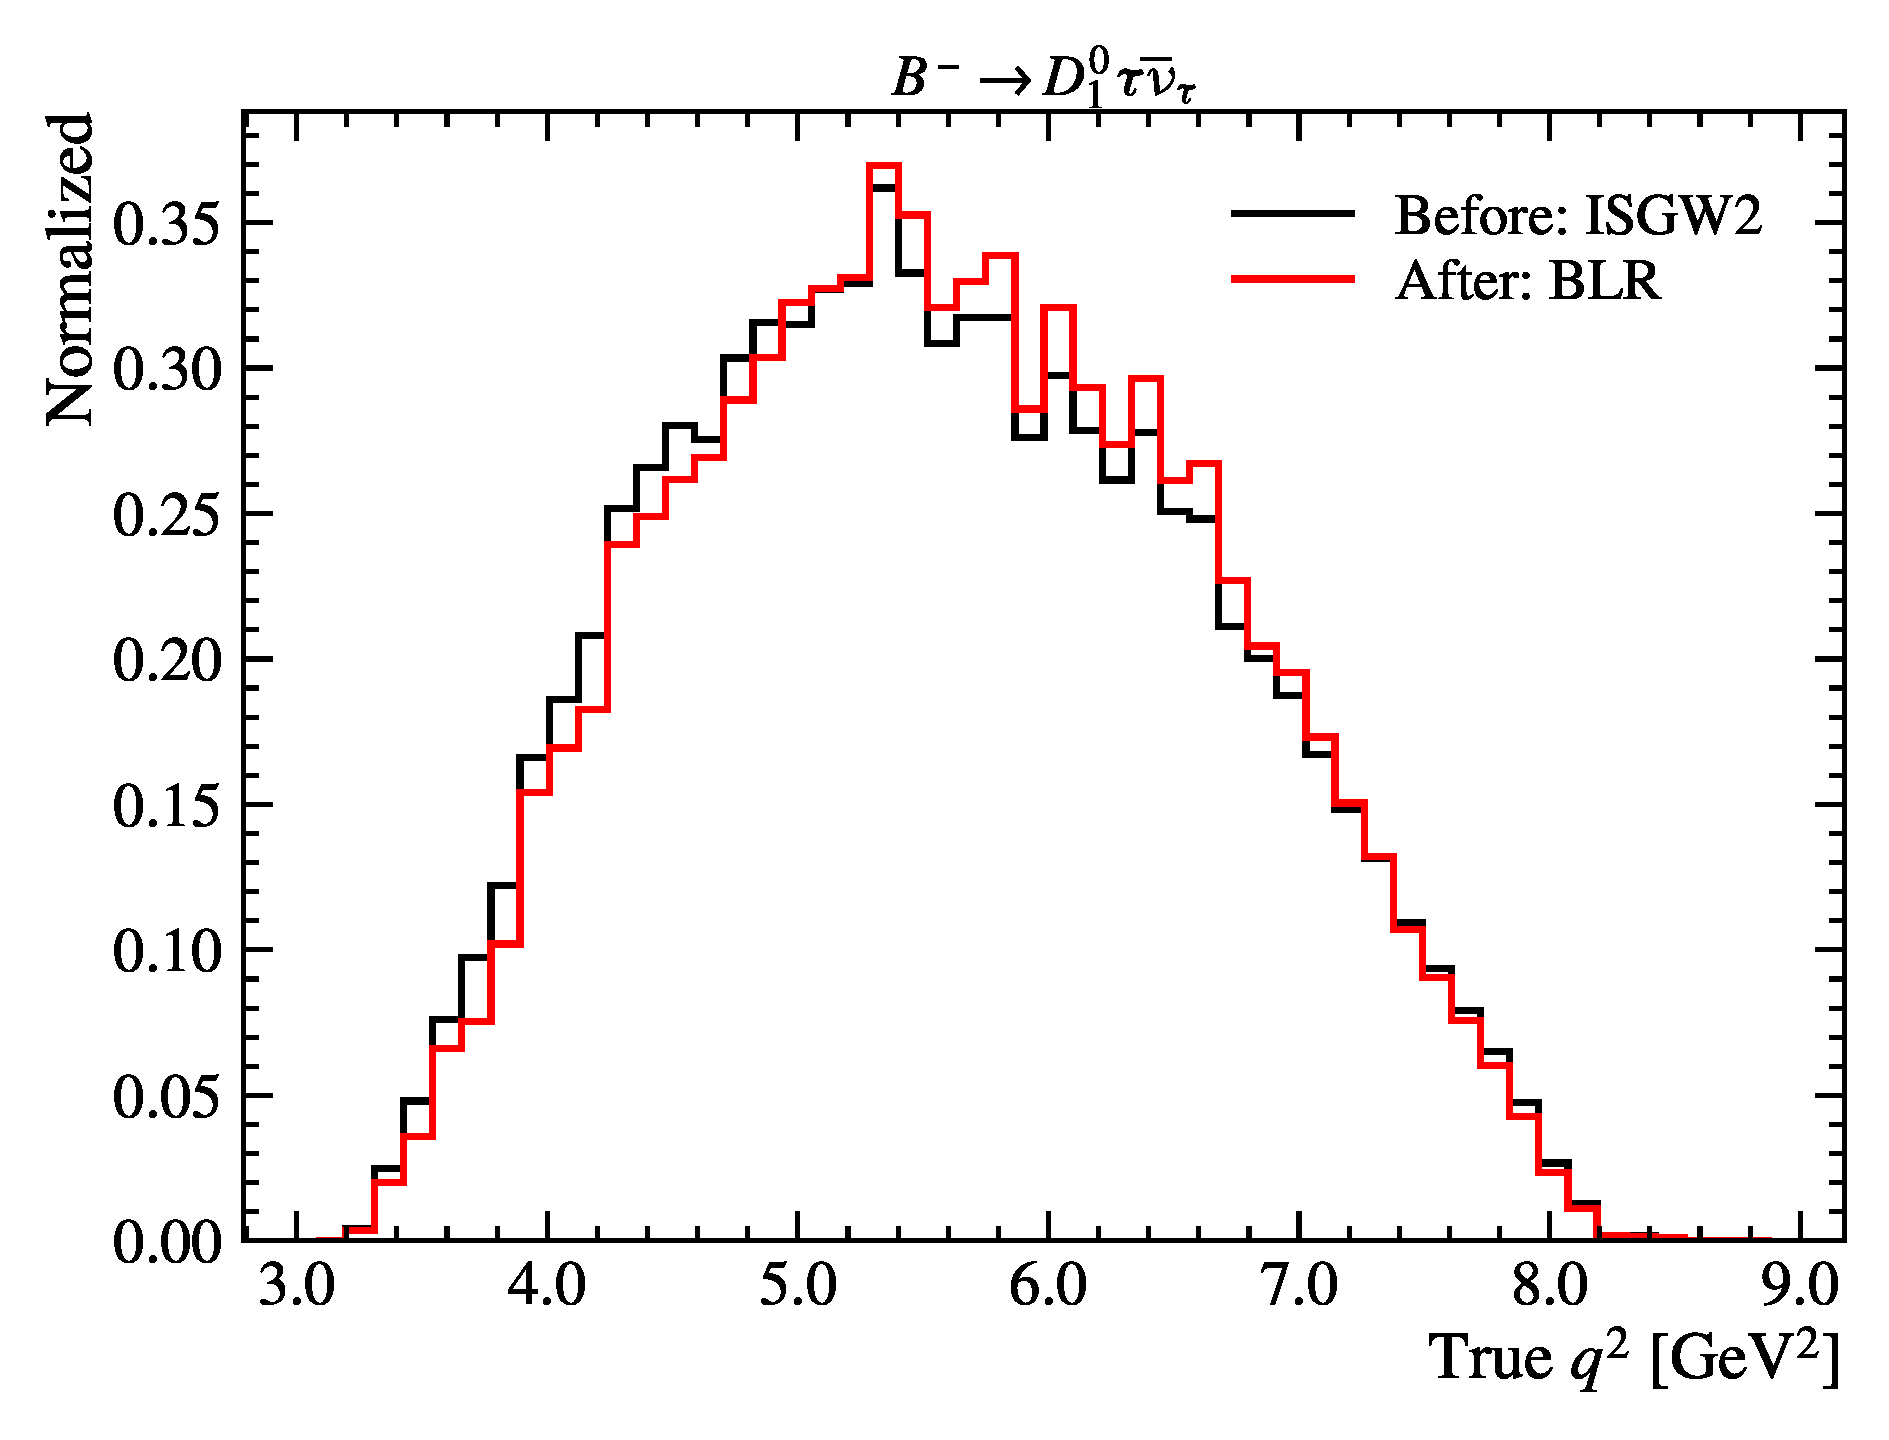
\includegraphics[width=0.24\textwidth]{
        ./figs-supplemental-plots/Dstst-form-factors/DststTau/D1stst0Tau.pdf
    }
    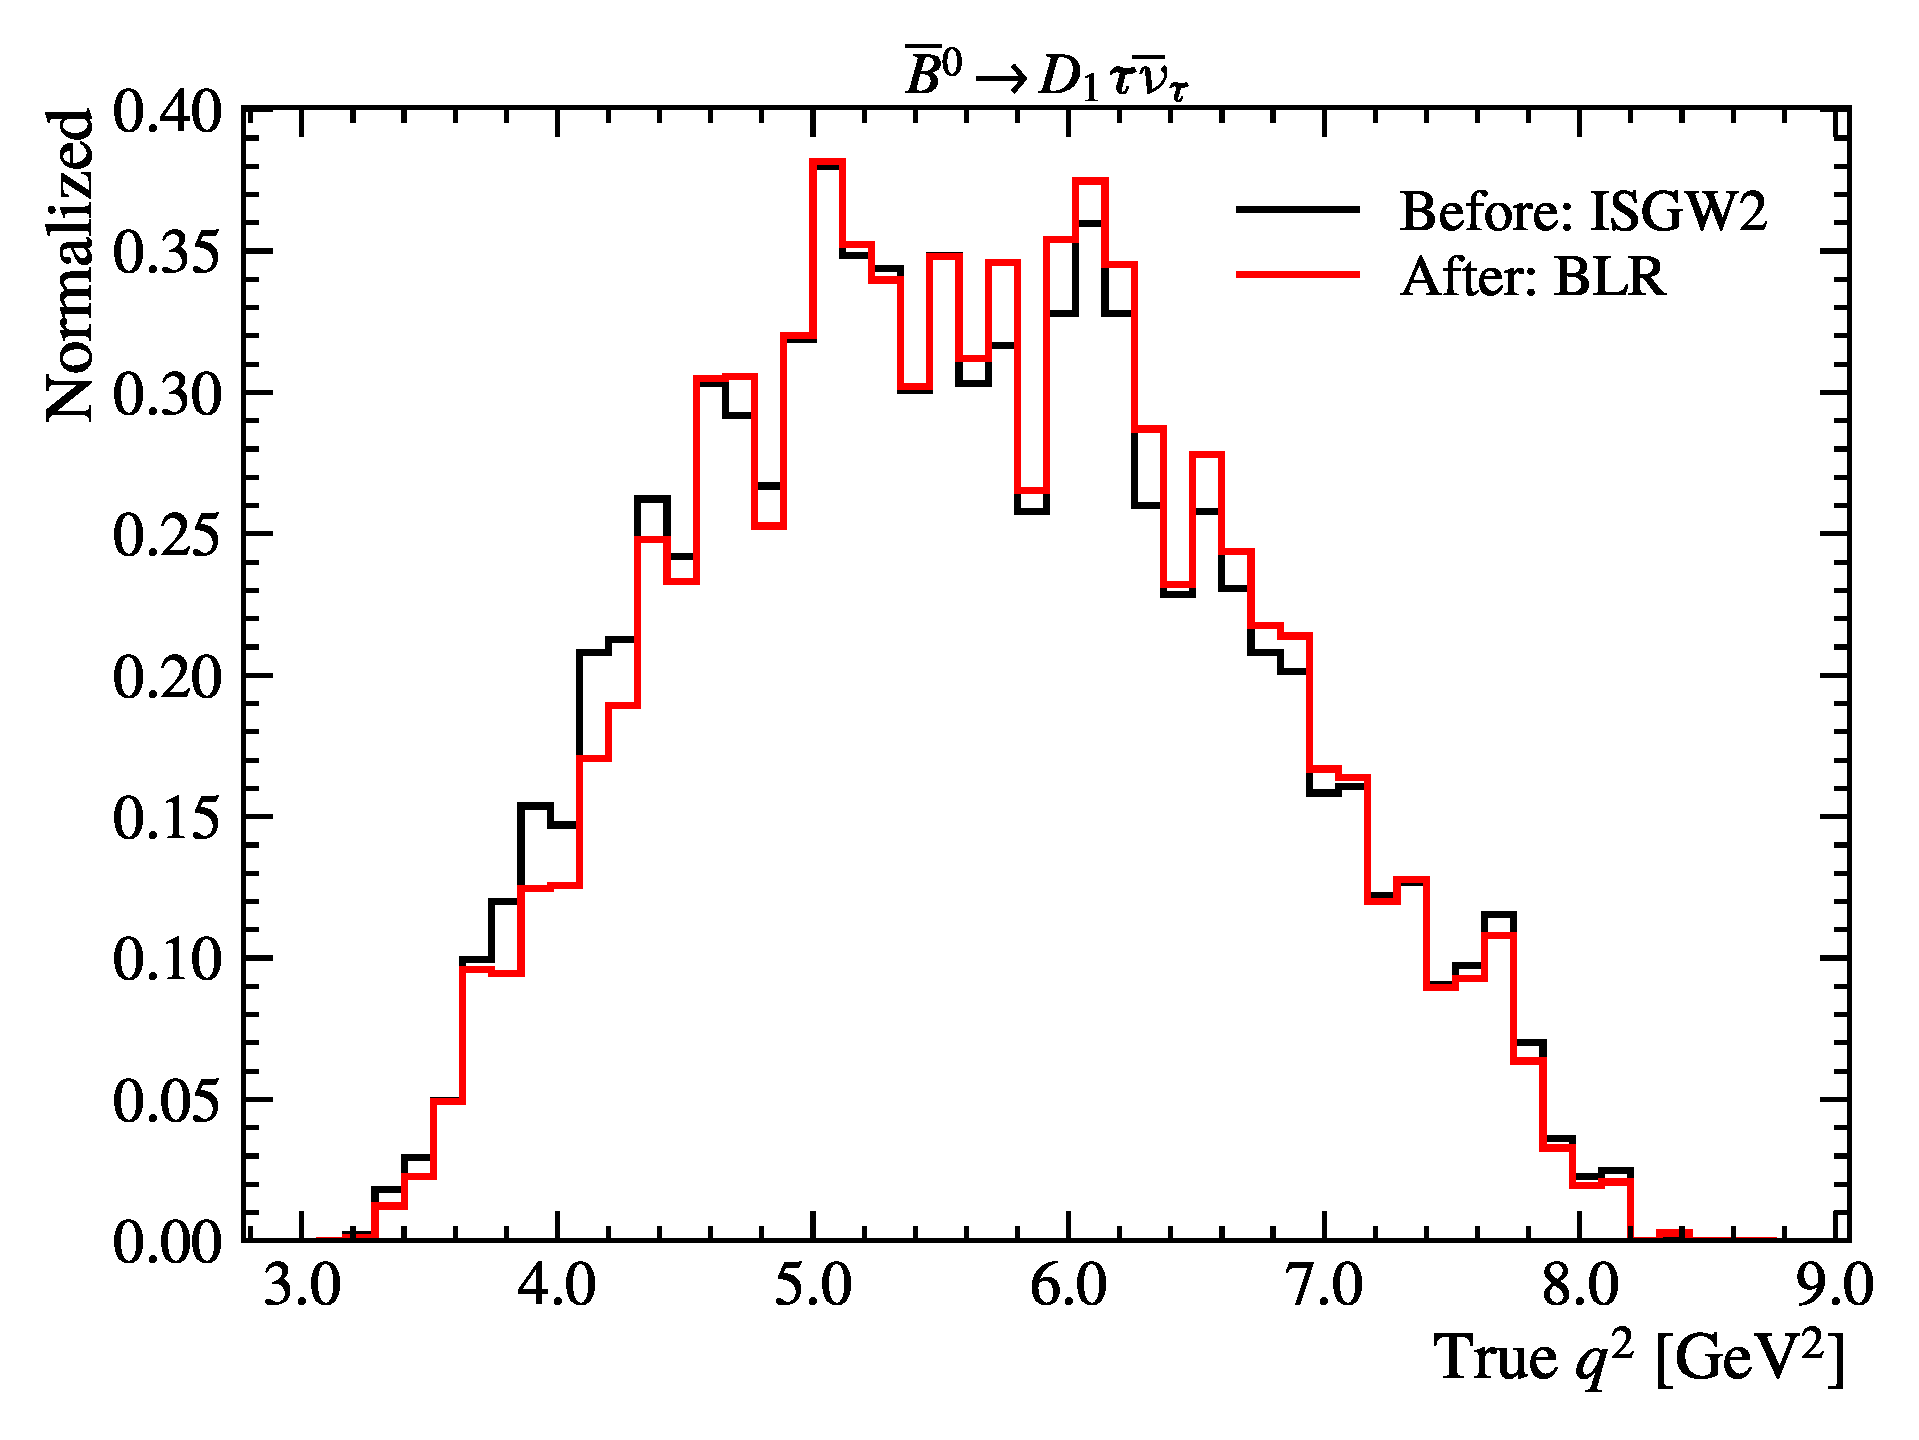
\includegraphics[width=0.24\textwidth]{
        ./figs-supplemental-plots/Dstst-form-factors/DststTau/D1ststTau.pdf
    }
    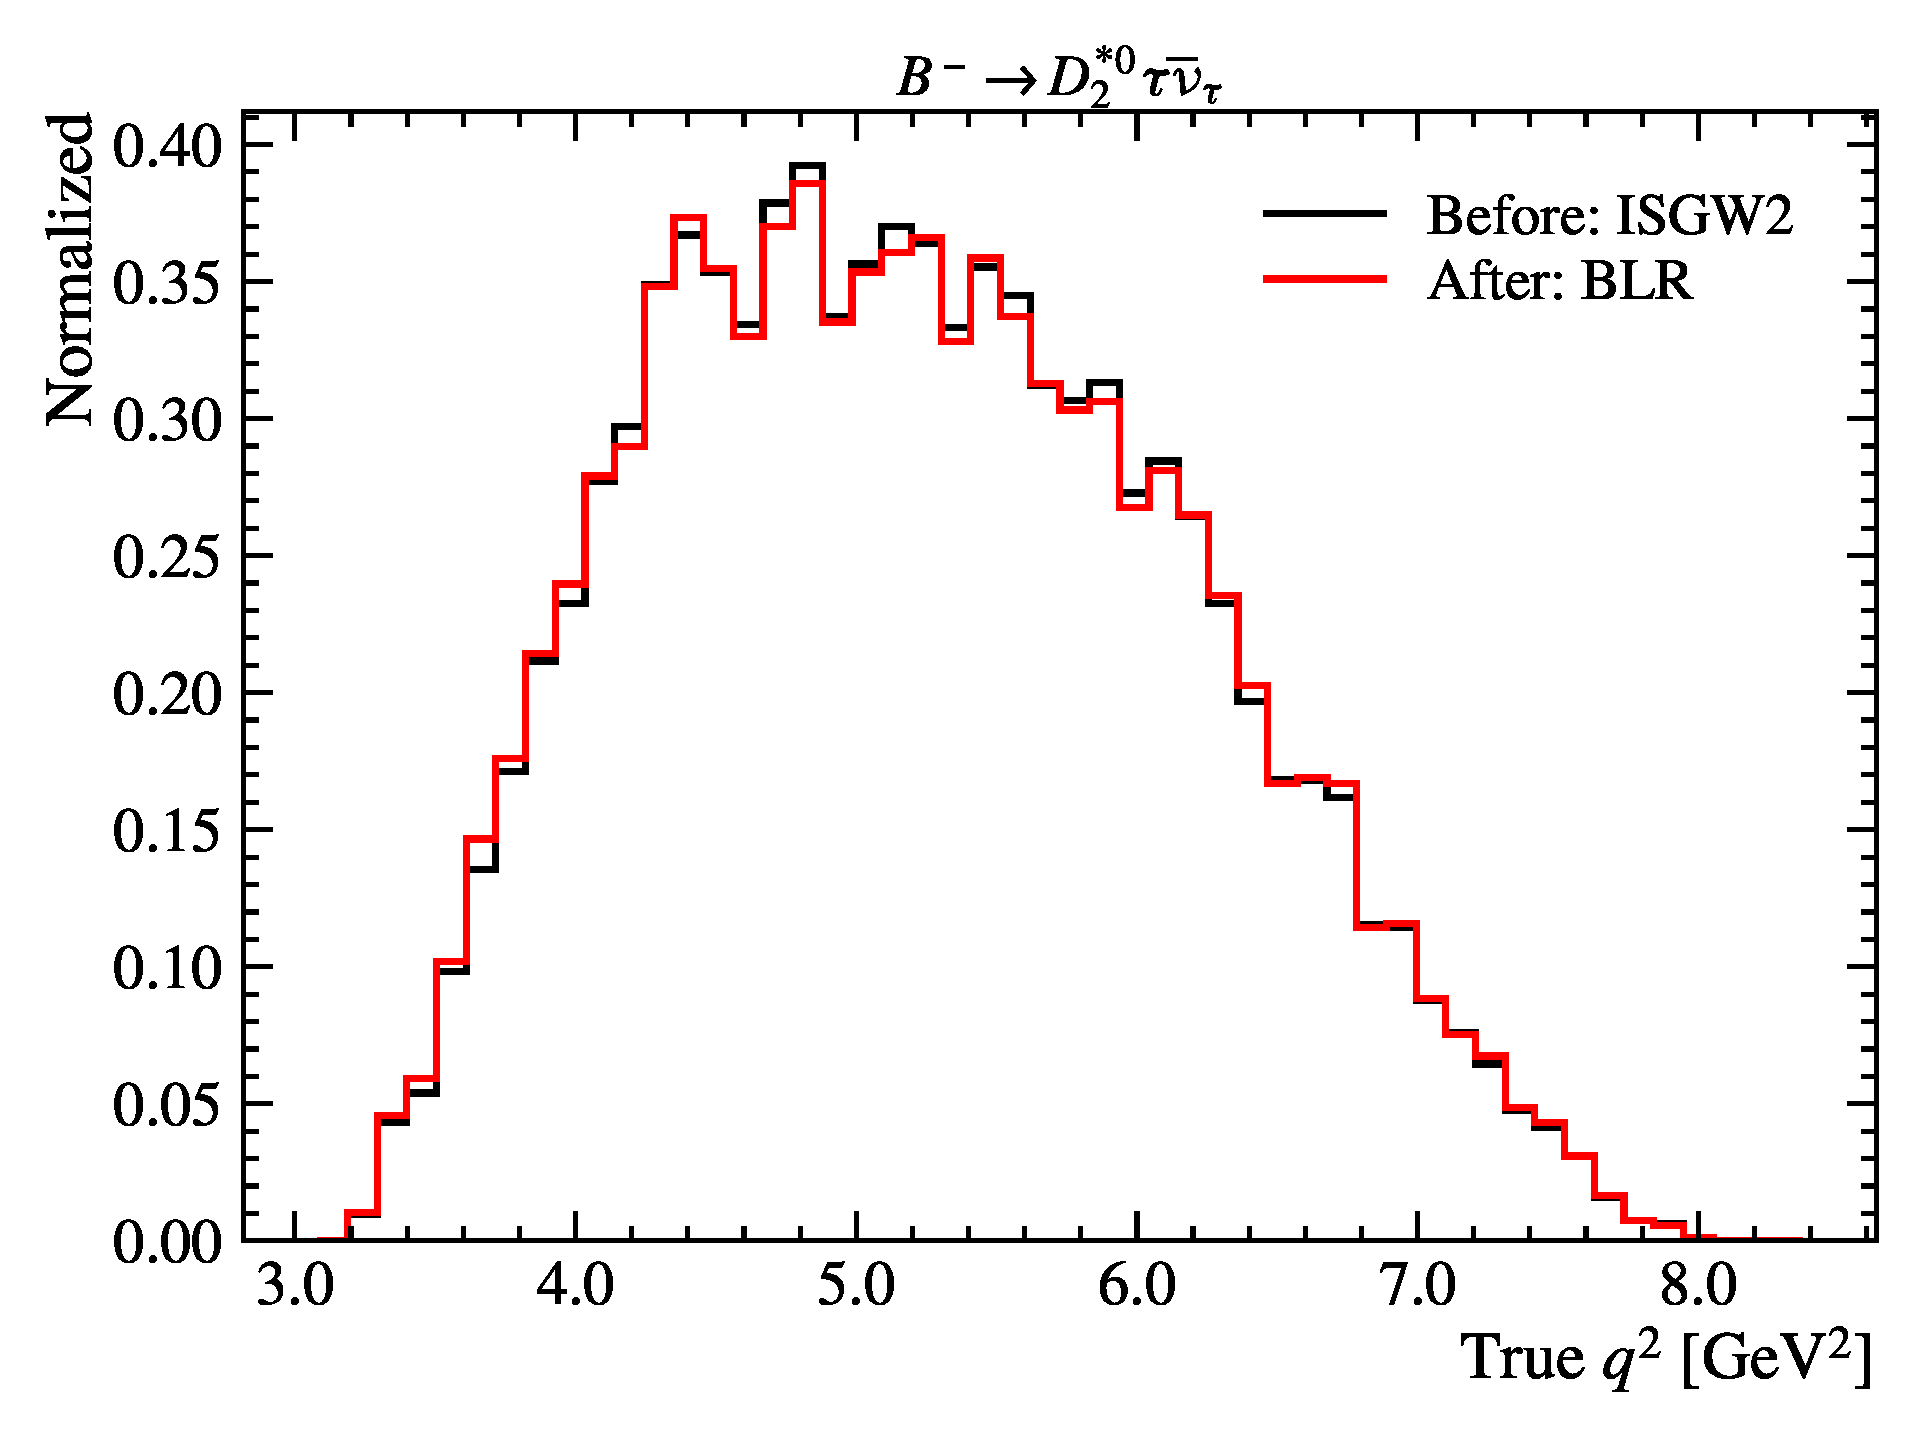
\includegraphics[width=0.24\textwidth]{
        ./figs-supplemental-plots/Dstst-form-factors/DststTau/D2stst0Tau.pdf
    }
    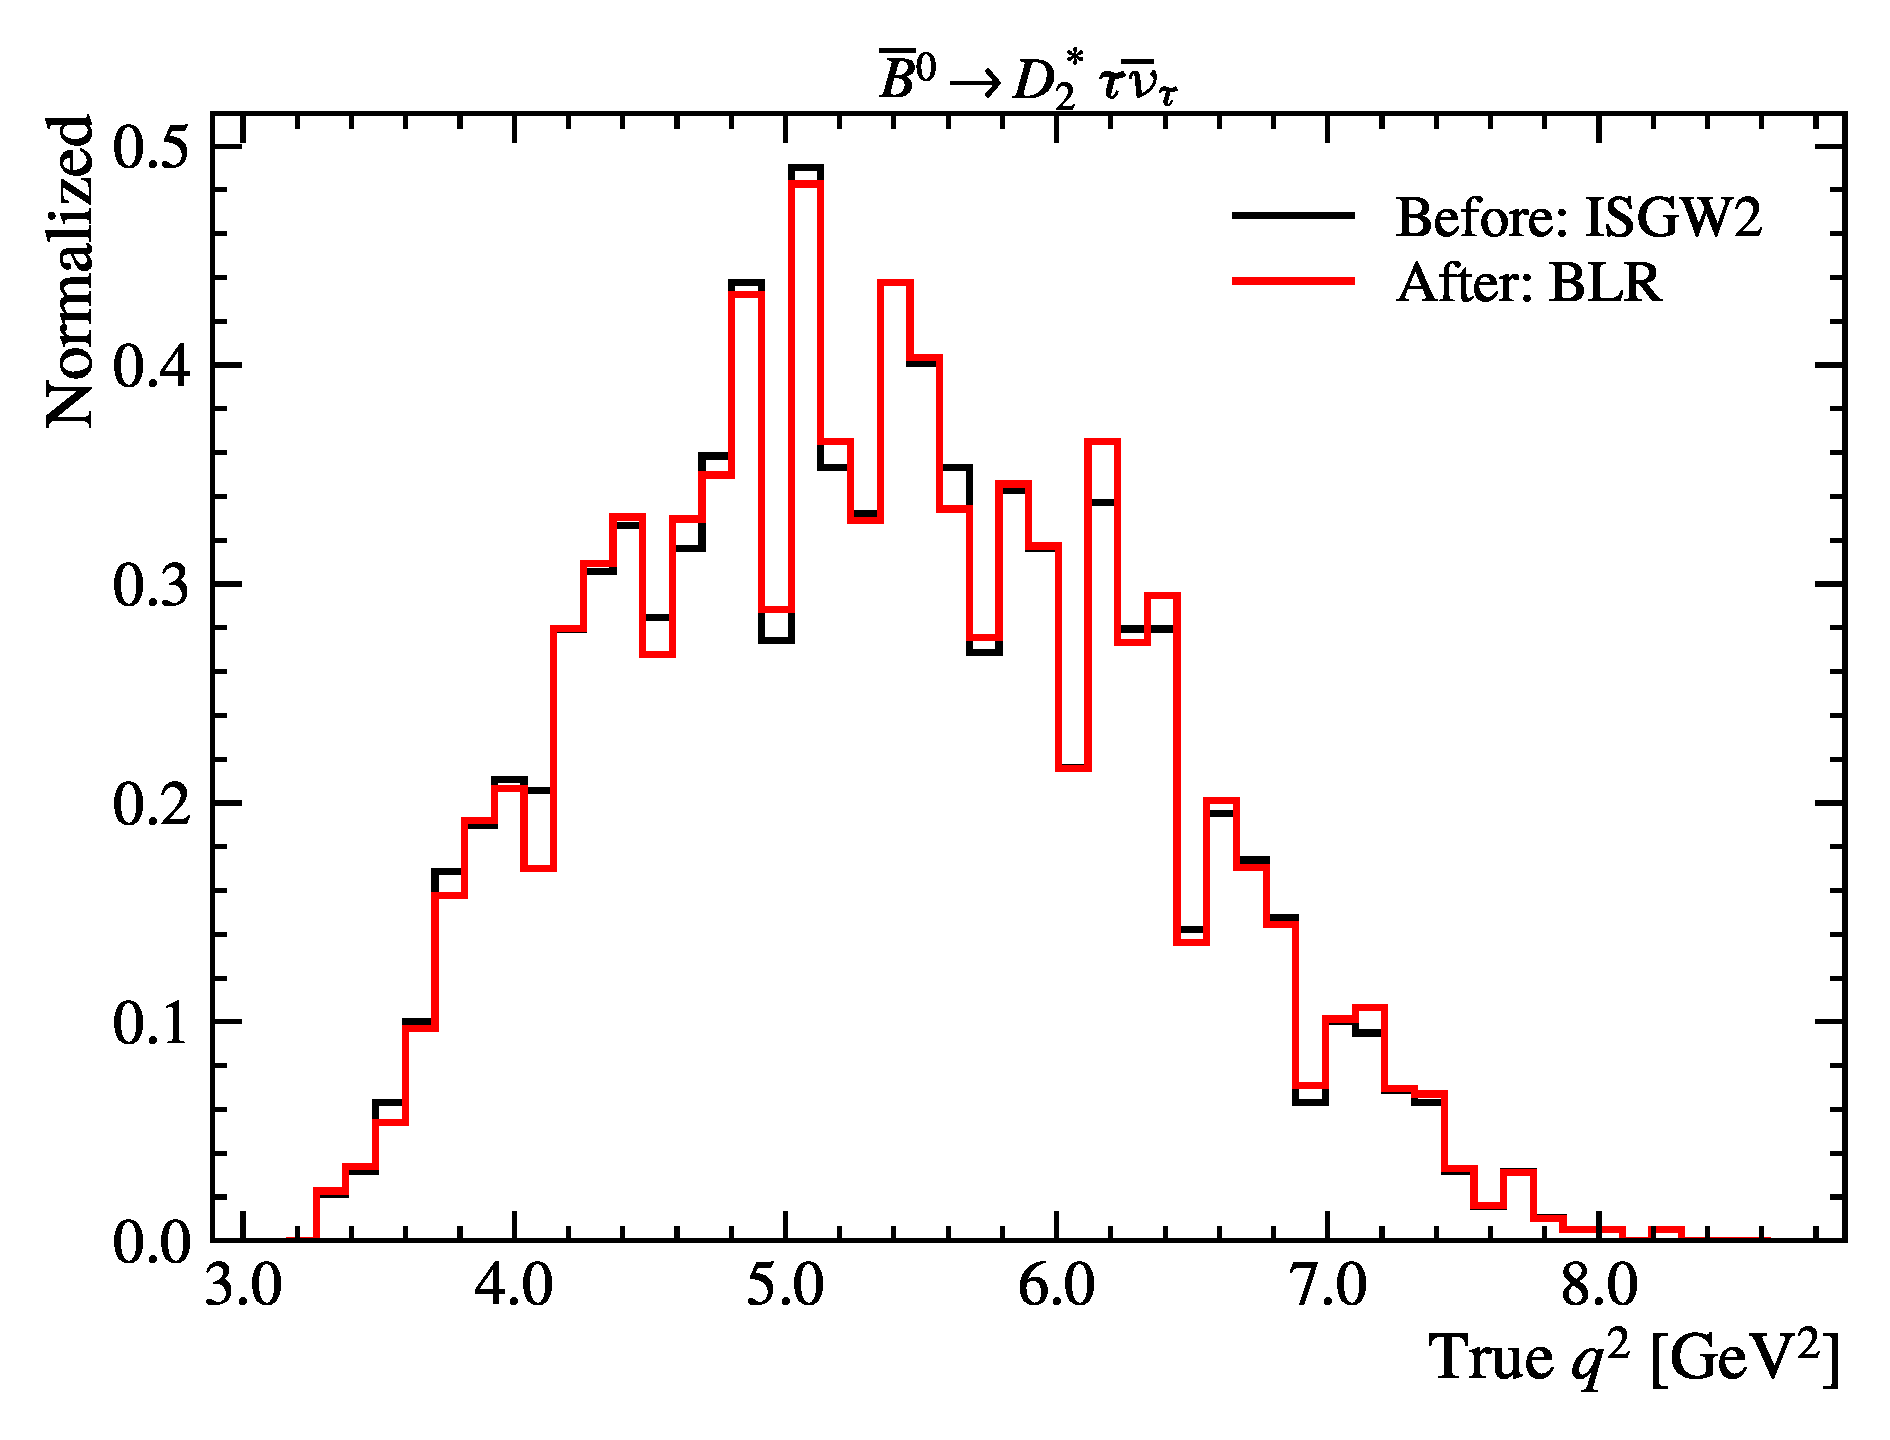
\includegraphics[width=0.24\textwidth]{
        ./figs-supplemental-plots/Dstst-form-factors/DststTau/D2ststTau.pdf
    }

    \caption{
        Form factor reweight effect on $D^{**}\tau$ MC templates.
        Parameters are taken verbatim from \cite{Bernlochner_2018}.
    }
    \label{fig:ff-rwt-raw-Dstst-sig-like}
\end{figure}


\section{\DstComb fit to 1OS, 2OS, and DD skims}
\label{appx:suppl:dst-comb}

The \DstComb\ fits to 1OS, 2OS, and DD skims are shown in
\cref{fig:dst-comb-fit-1os,fig:dst-comb-fit-2os,fig:dst-comb-fit-dd}.
The effects of scaling are displayed in
\cref{fig:dst-comb-scale-other-skims}.

\begin{figure}[htb]
    \centering
    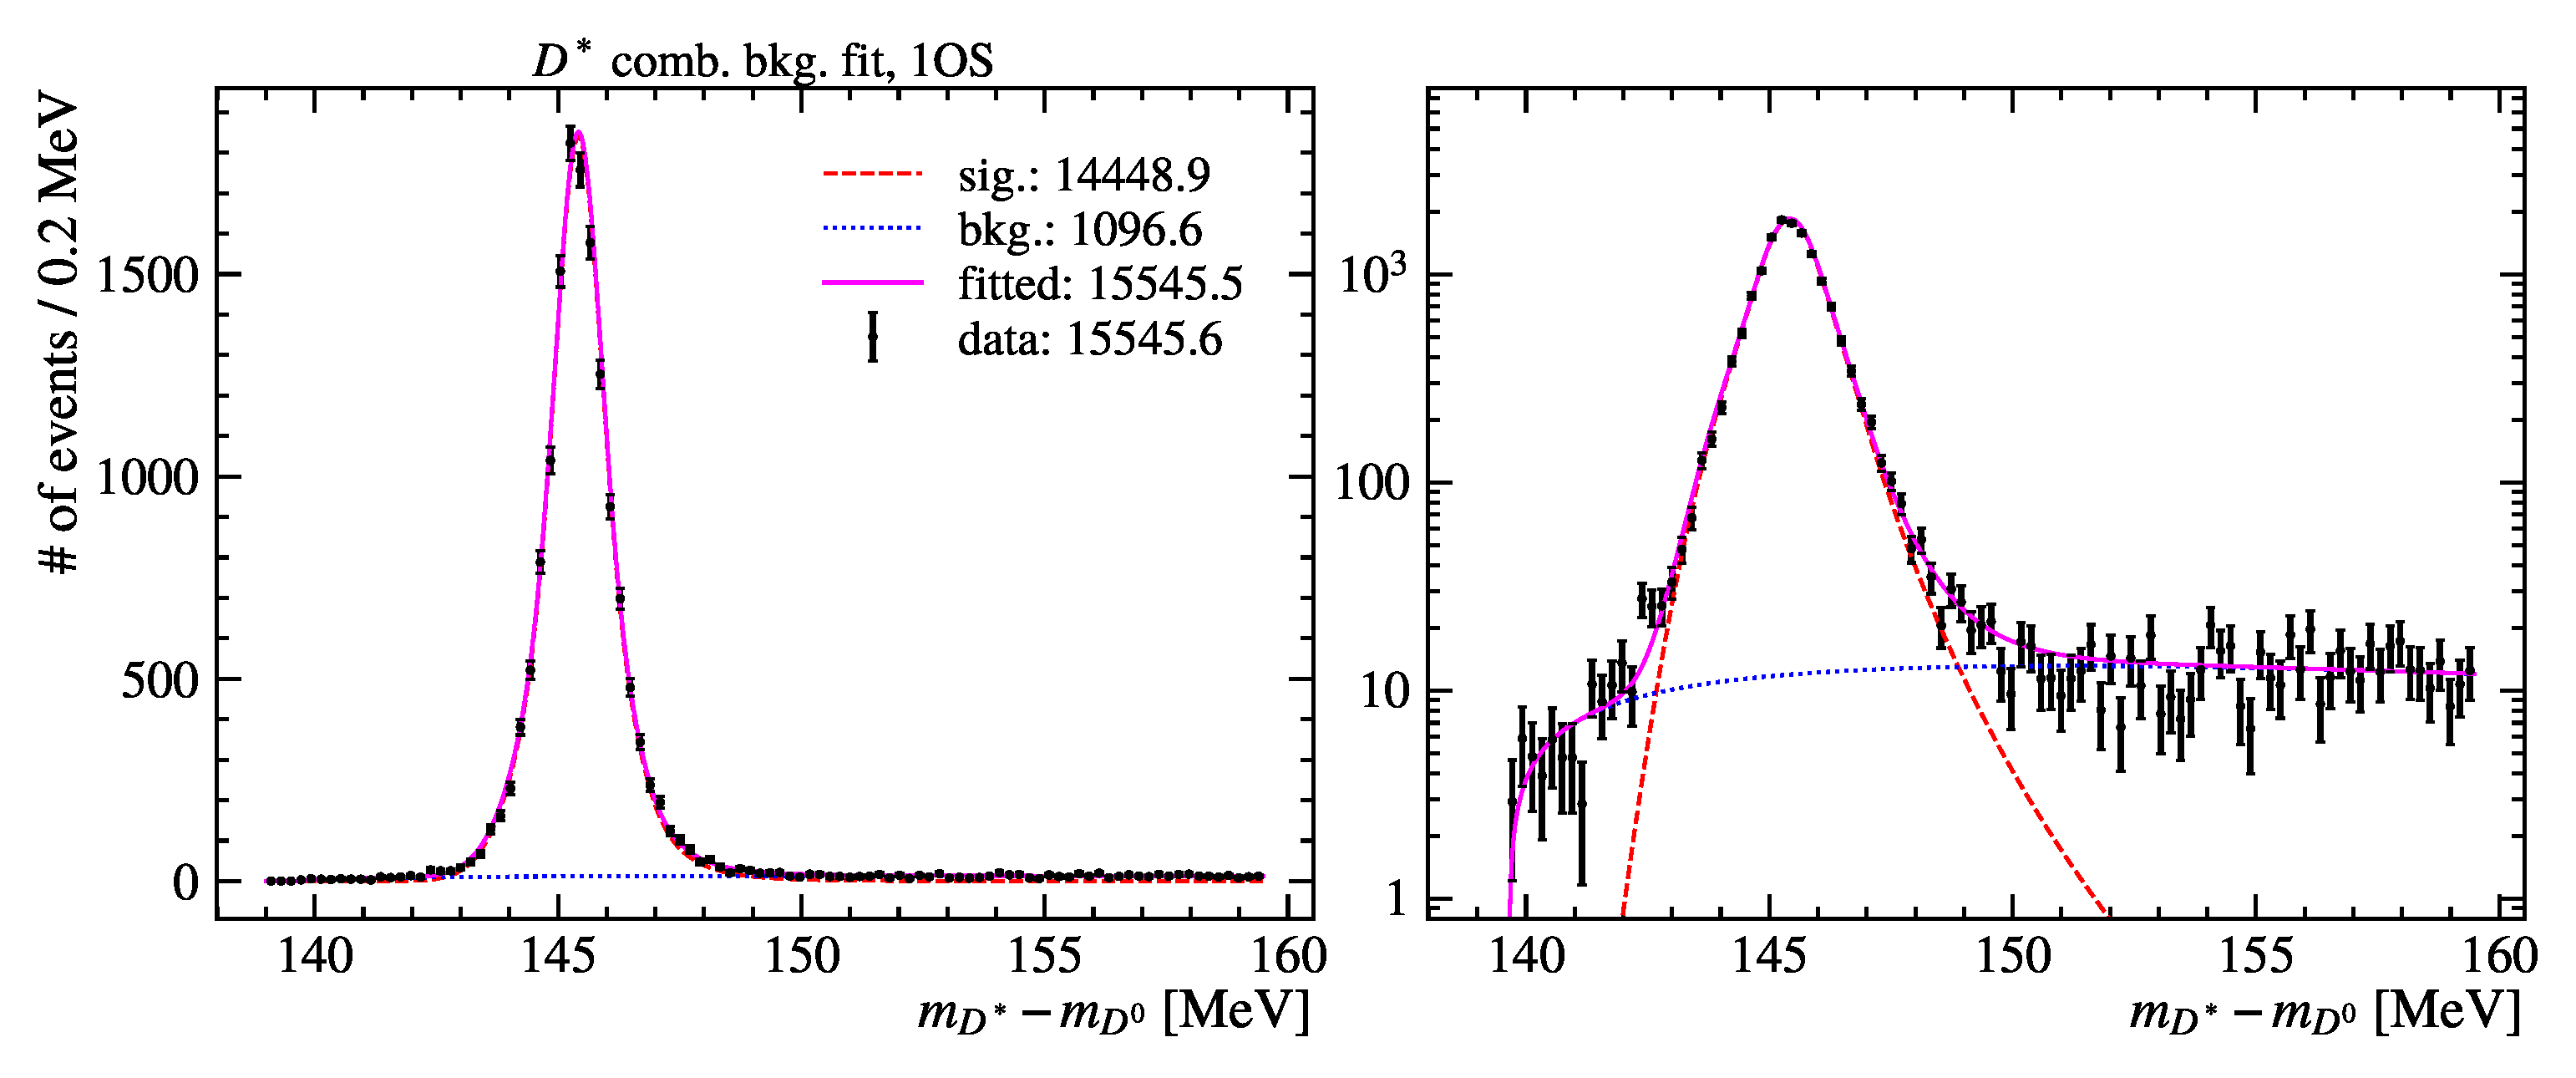
\includegraphics[width=\textwidth]{figs-fit-fit-templates/data-driven-plots/dst_comb/fit_dst_comb_1os_comb.pdf}
    \caption{
        \DstComb\ auxiliary fit to the 1OS skim.
    }
    \label{fig:dst-comb-fit-1os}
\end{figure}

\begin{figure}[htb]
    \centering
    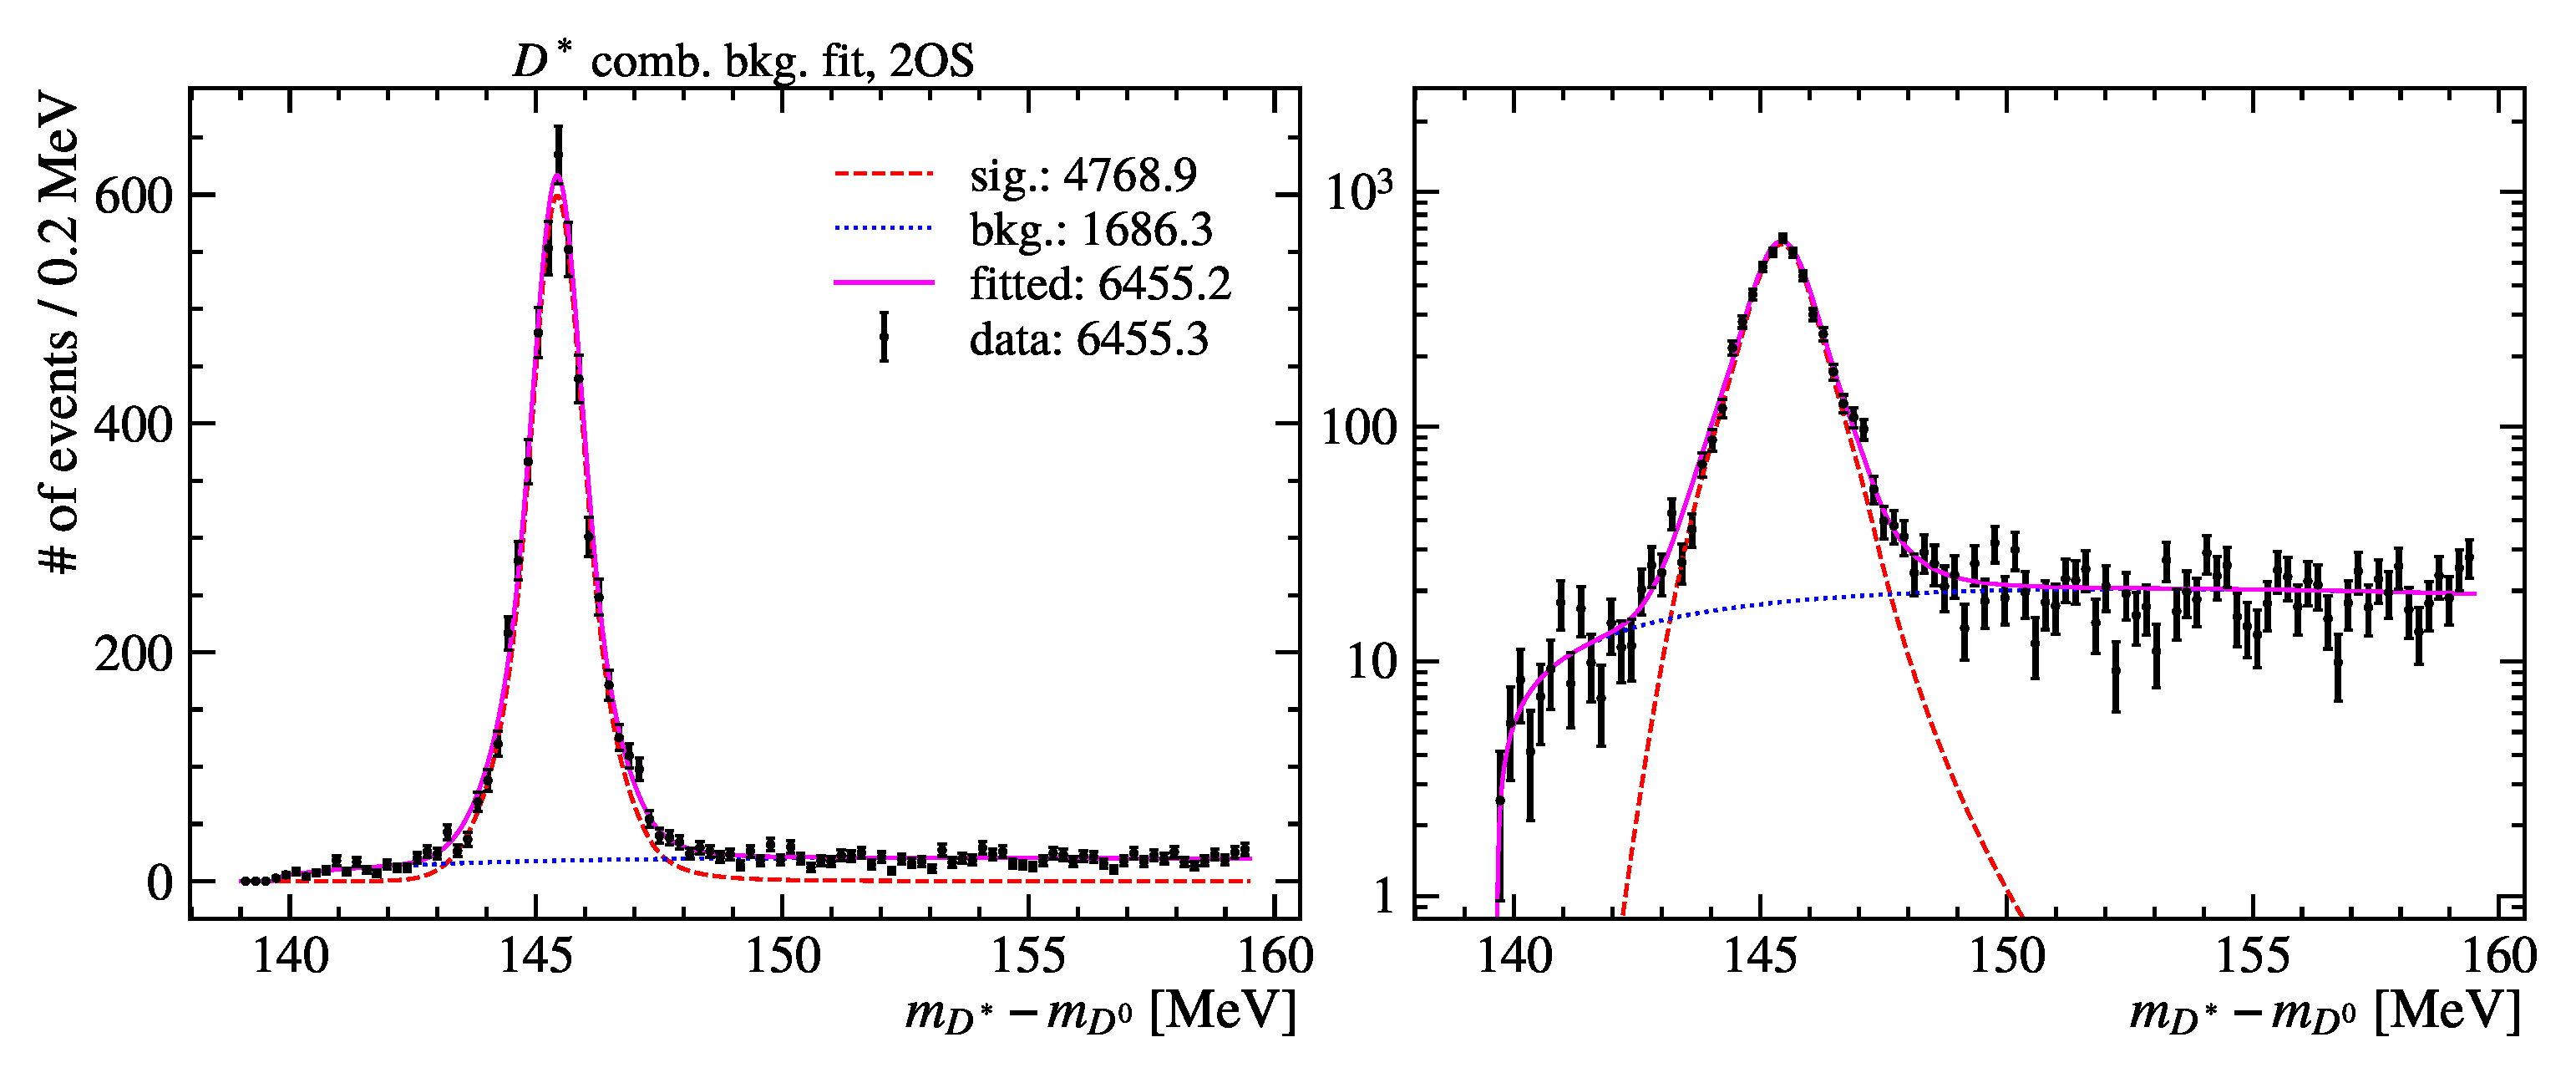
\includegraphics[width=\textwidth]{figs-fit-fit-templates/data-driven-plots/dst_comb/fit_dst_comb_2os_comb.pdf}
    \caption{
        \DstComb\ auxiliary fit to the 2OS skim.
    }
    \label{fig:dst-comb-fit-2os}
\end{figure}

\begin{figure}[htb]
    \centering
    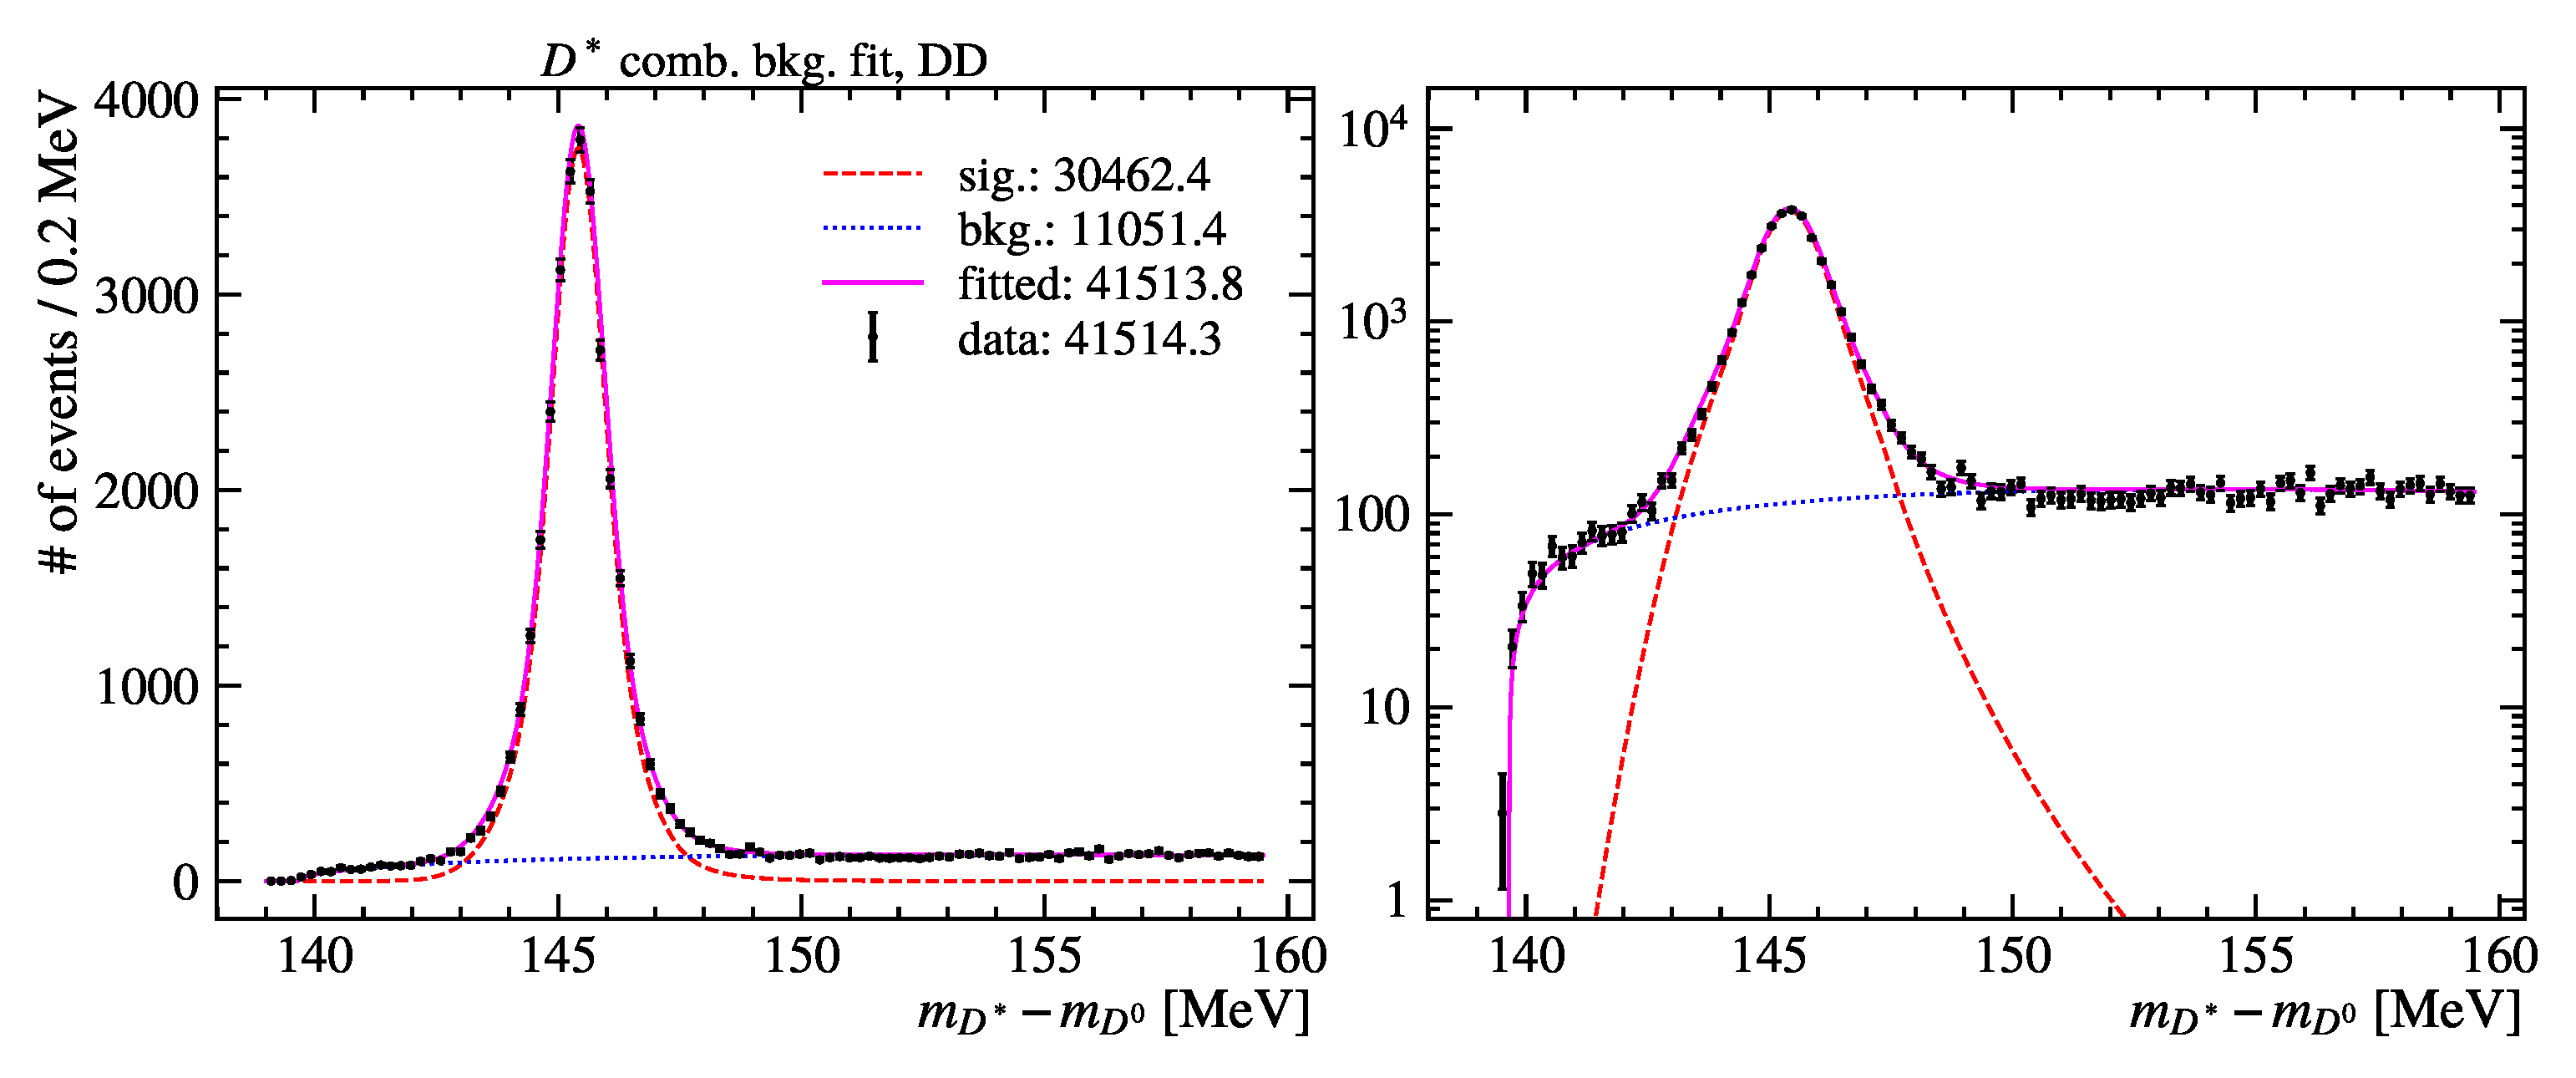
\includegraphics[width=\textwidth]{figs-fit-fit-templates/data-driven-plots/dst_comb/fit_dst_comb_dd_comb.pdf}
    \caption{
        \DstComb\ auxiliary fit to the DD skim.
    }
    \label{fig:dst-comb-fit-dd}
\end{figure}

\begin{figure}[htb]
    \centering
    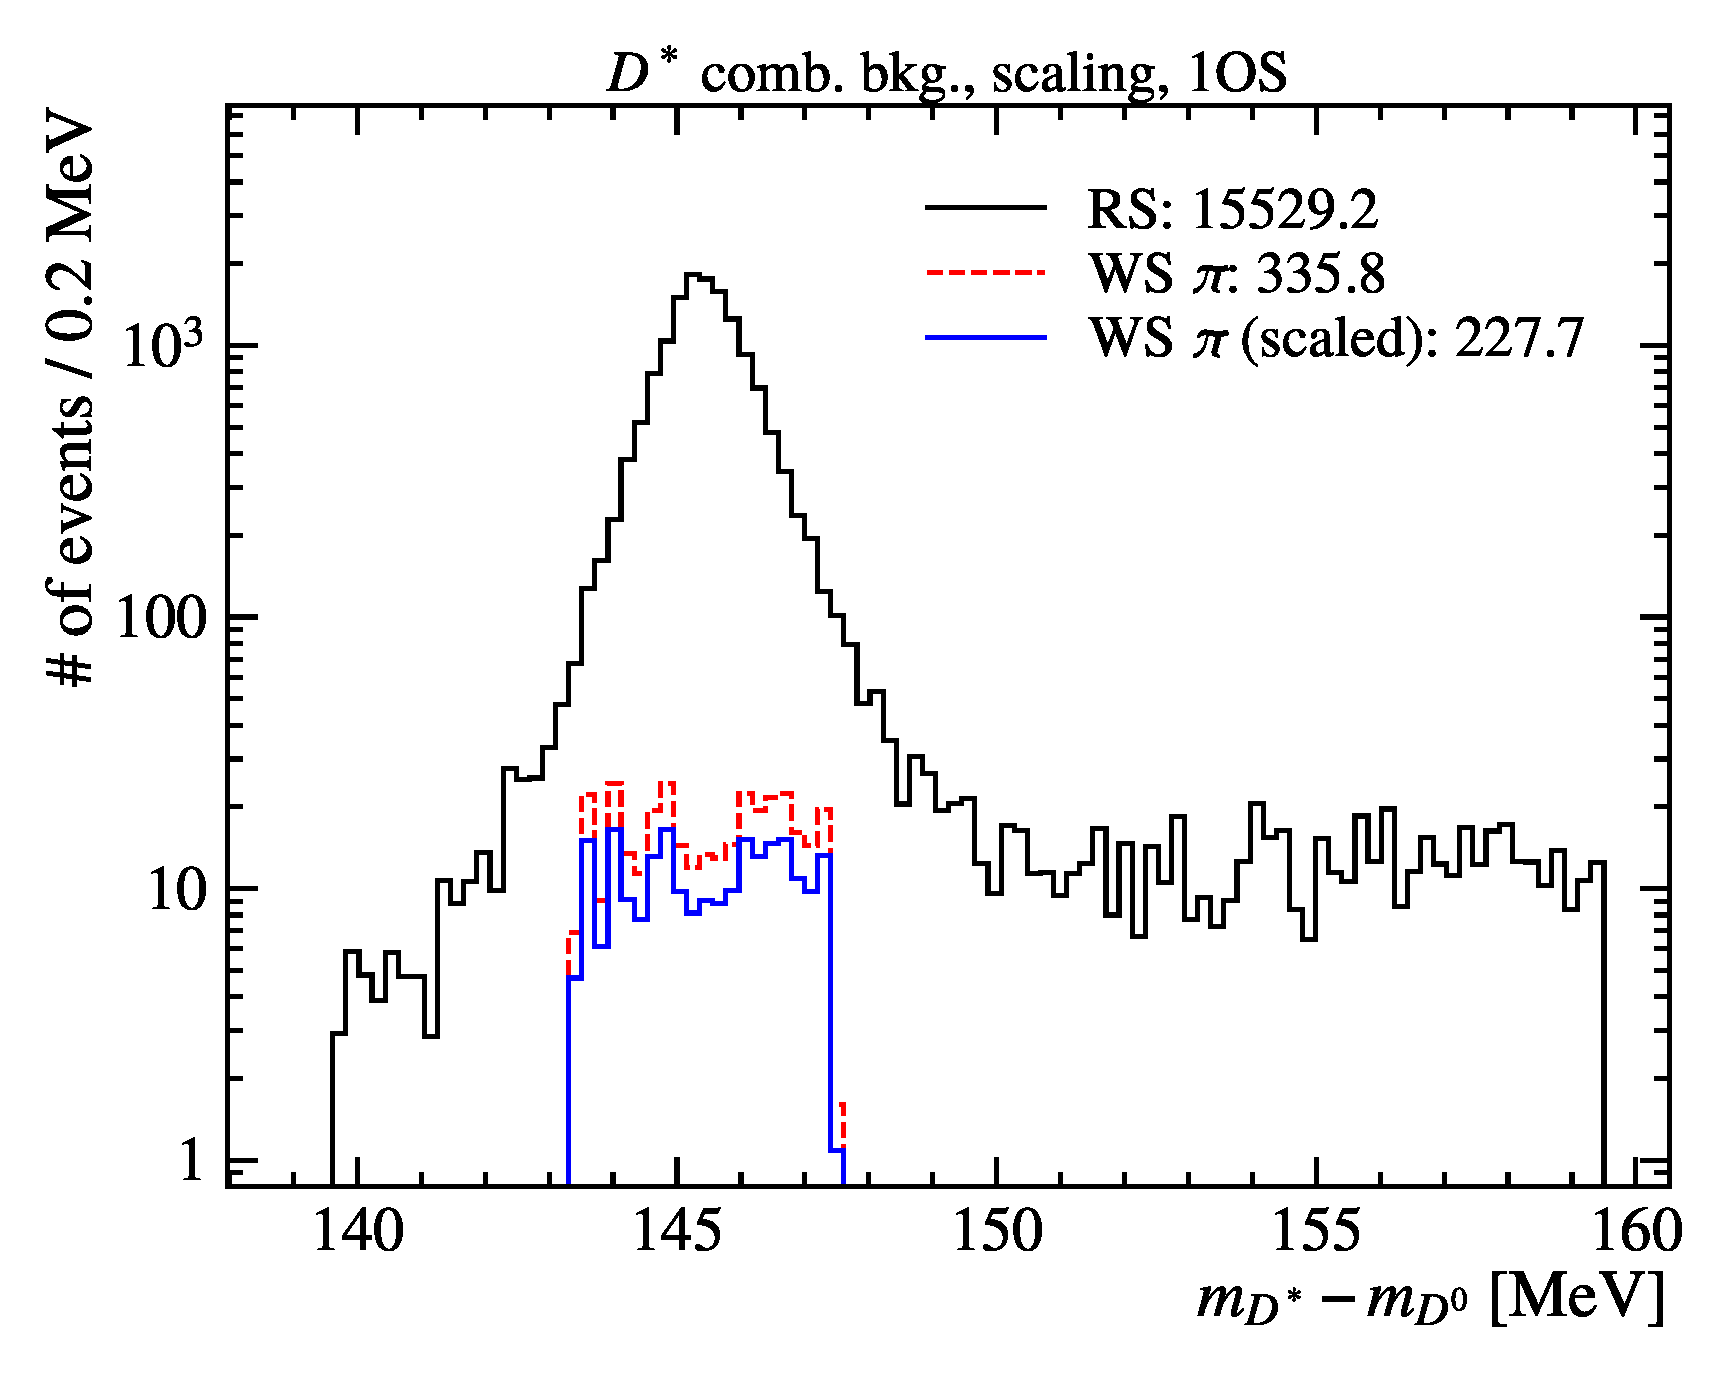
\includegraphics[width=0.32\textwidth]{figs-fit-fit-templates/data-driven-plots/dst_comb/fit_dst_comb_scaled_comp_1os_log.pdf}
    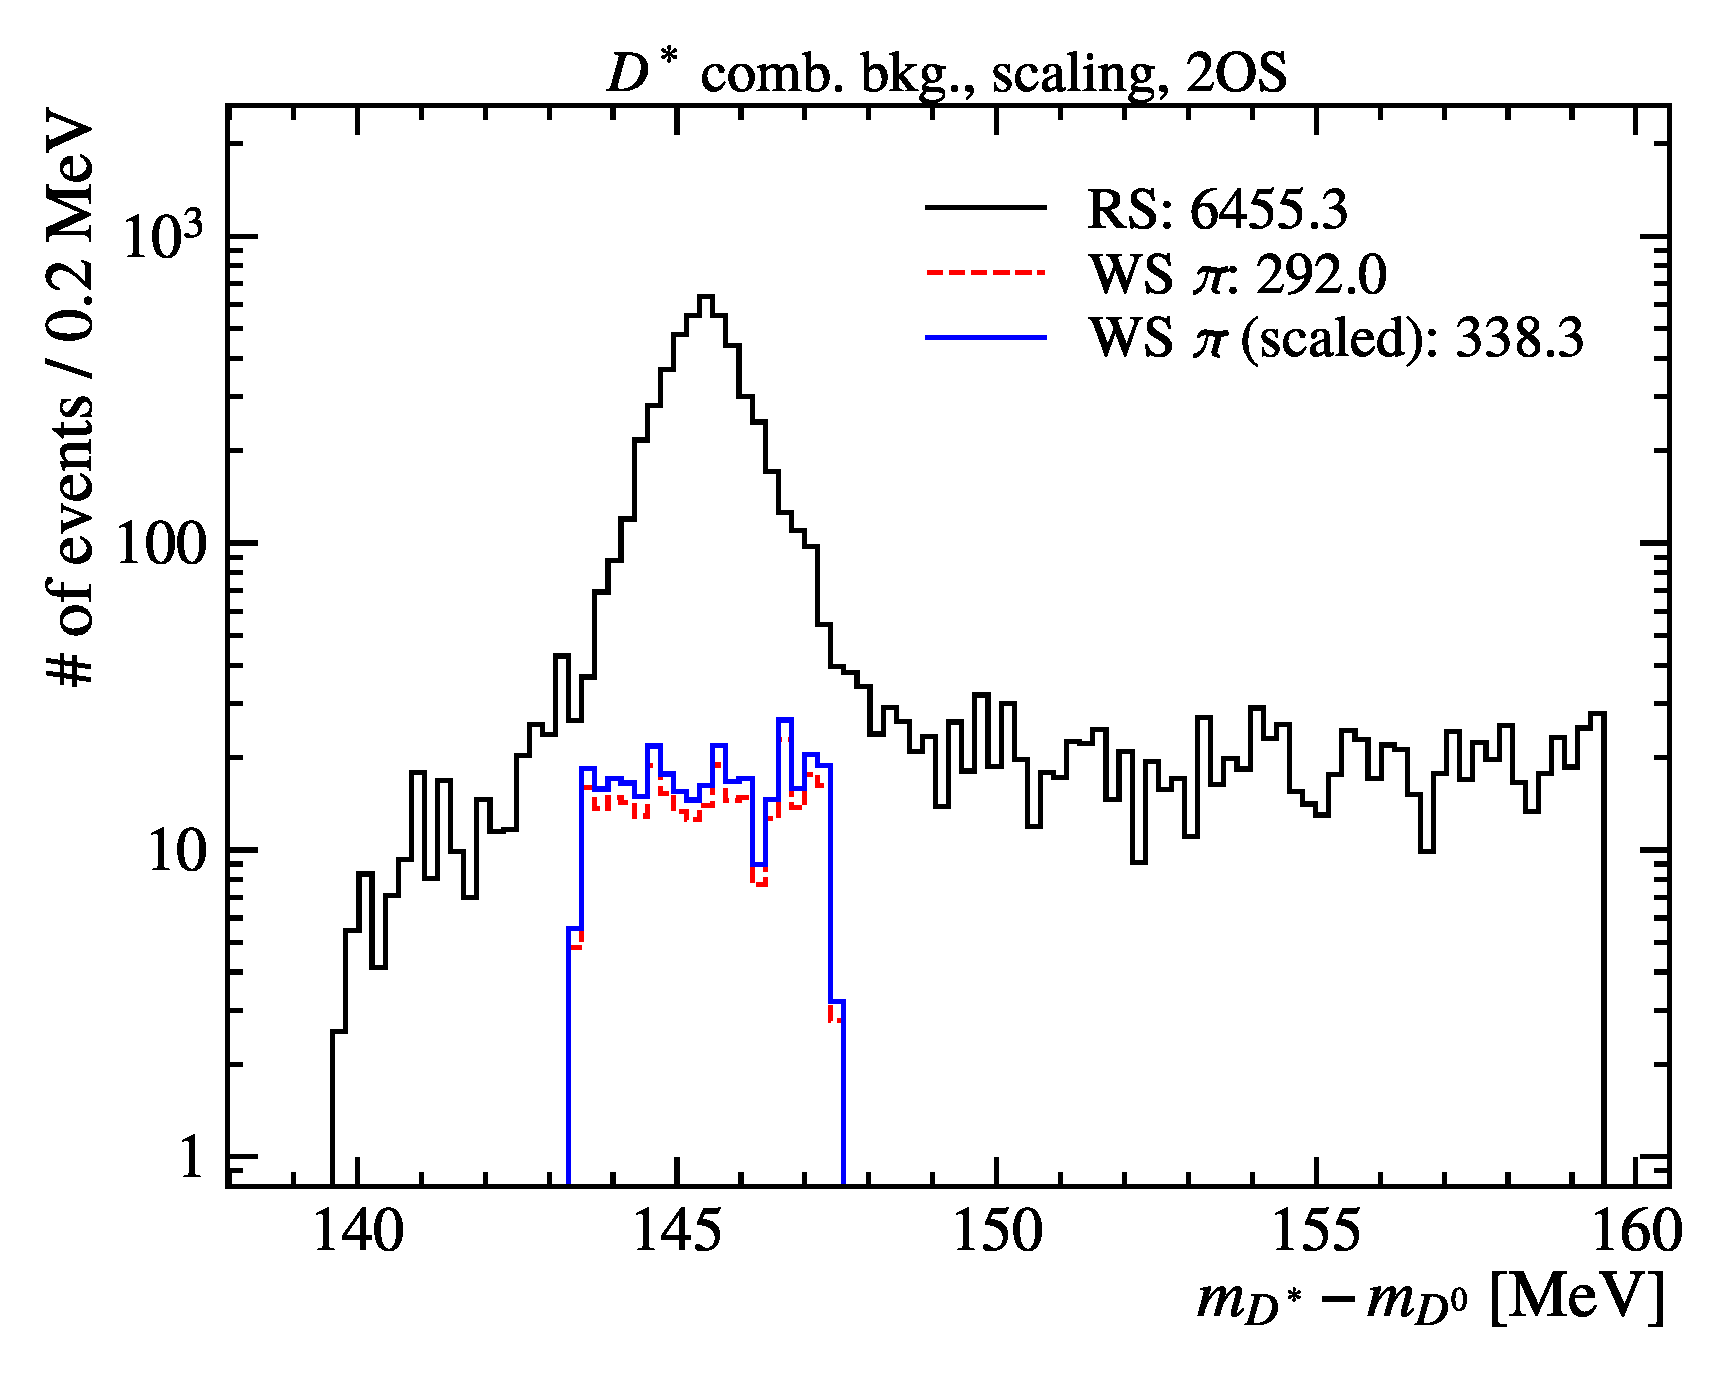
\includegraphics[width=0.32\textwidth]{figs-fit-fit-templates/data-driven-plots/dst_comb/fit_dst_comb_scaled_comp_2os_log.pdf}
    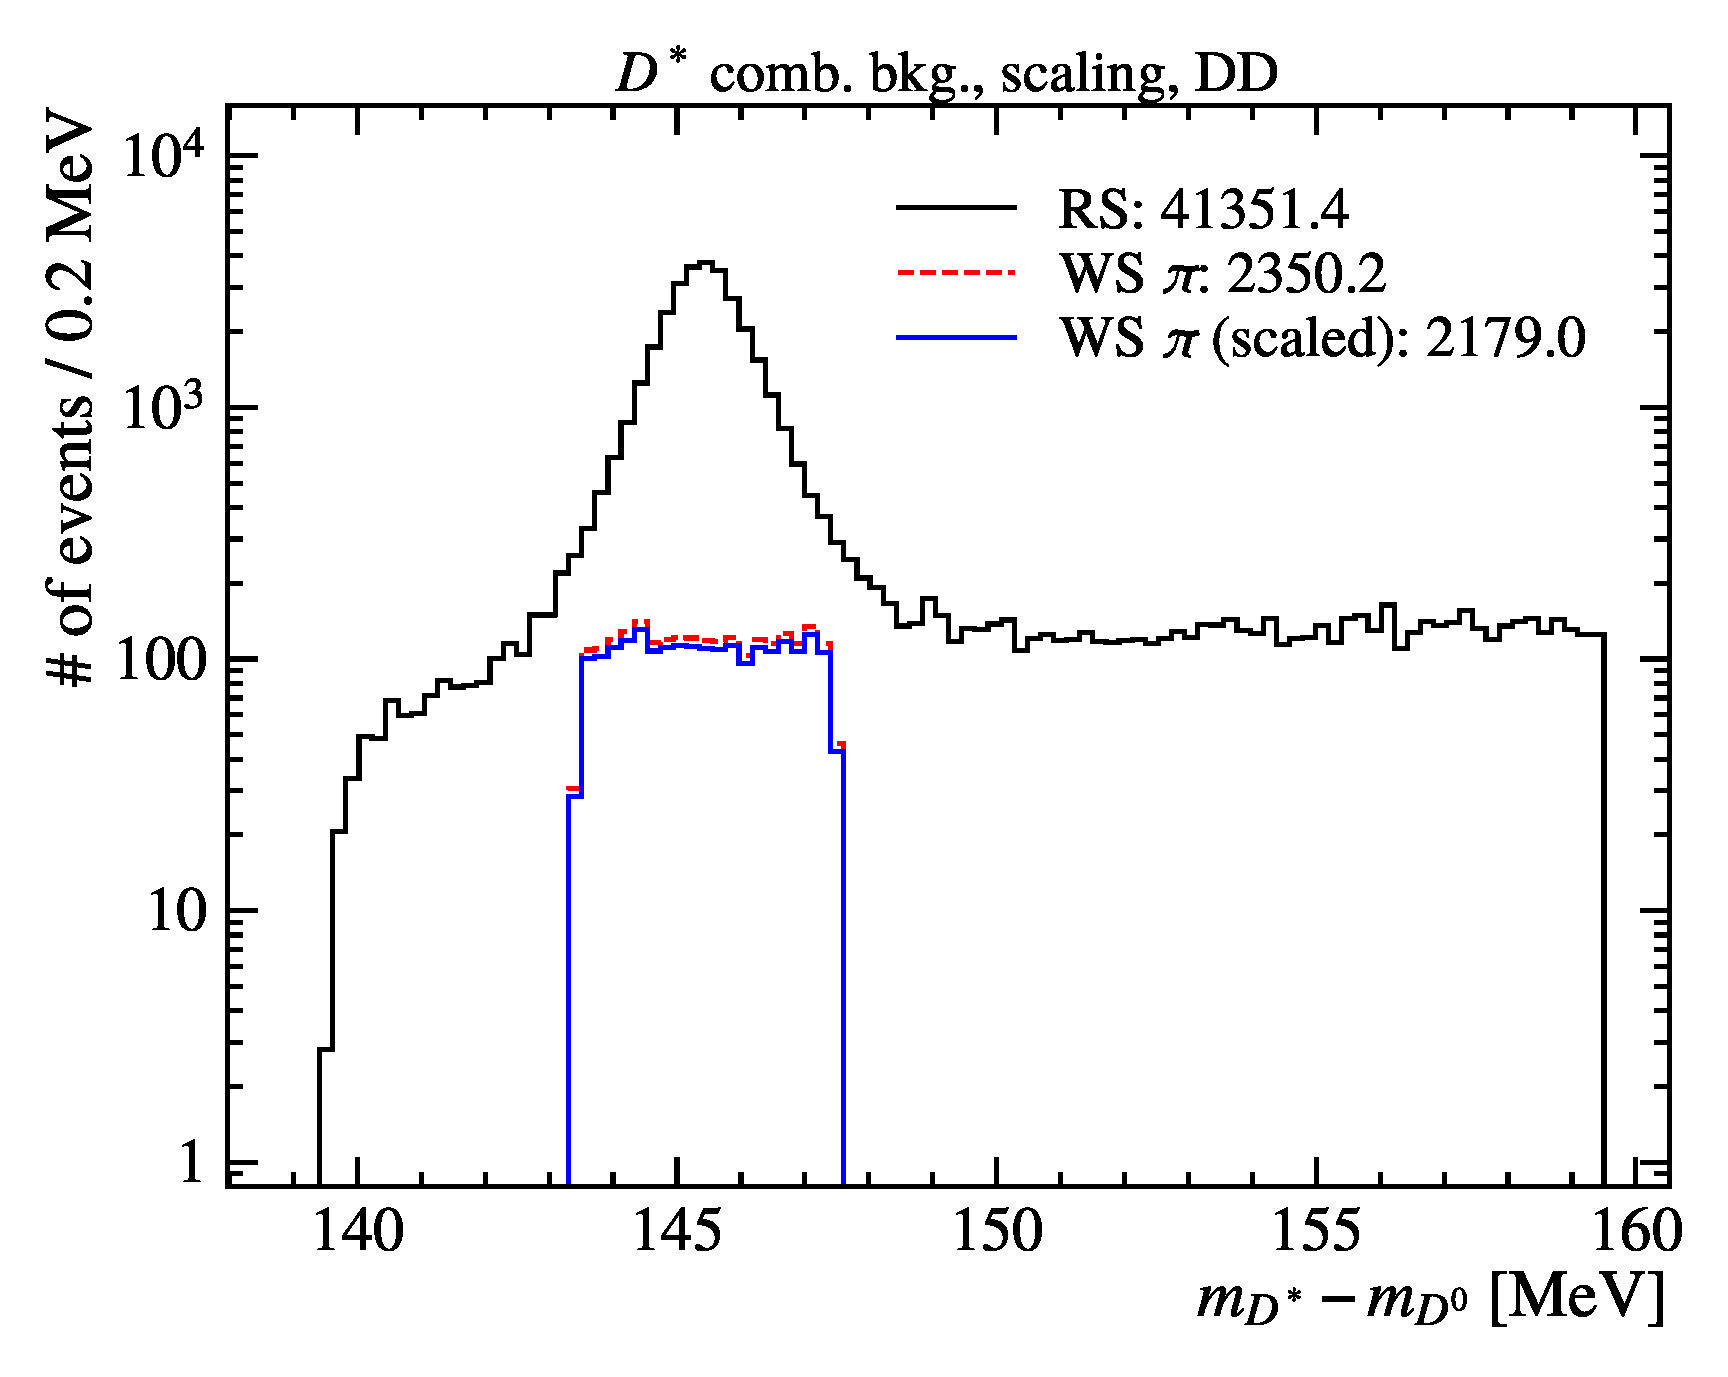
\includegraphics[width=0.32\textwidth]{figs-fit-fit-templates/data-driven-plots/dst_comb/fit_dst_comb_scaled_comp_dd_log.pdf}

    \caption{
        Effect of scaling for the 1OS, 2OS, and DD skims on the \DstComb\
        templates.
    }
    \label{fig:dst-comb-scale-other-skims}
\end{figure}


\section{Compare L0Global TIS efficiencies in MC with TISTOS method}
\label{appx:suppl:l0global-tis}

It is discussed that
$\epsilon_\text{TISTOS} = \epsilon_\text{TIS}$ in $B \rightarrow \jpsi K$ MC,
thus TISTOS method works (on $\jpsi K$).

We show in \cref{fig:check-l0global-tis-with-tistos} that TISTOS method does not
work in our MC samples.
Therefore, in the main text, we use \cref{eqn:eff-l0global-tis} to compute
efficiencies in MC.

% Generated in /lhcb-ntuples-gen/studies/trigger_emulation-l0_global_tis_debug:
% By running:
%   debug_l0global.py
% in the folder specified above.
\begin{figure}[ht]
    \centering
    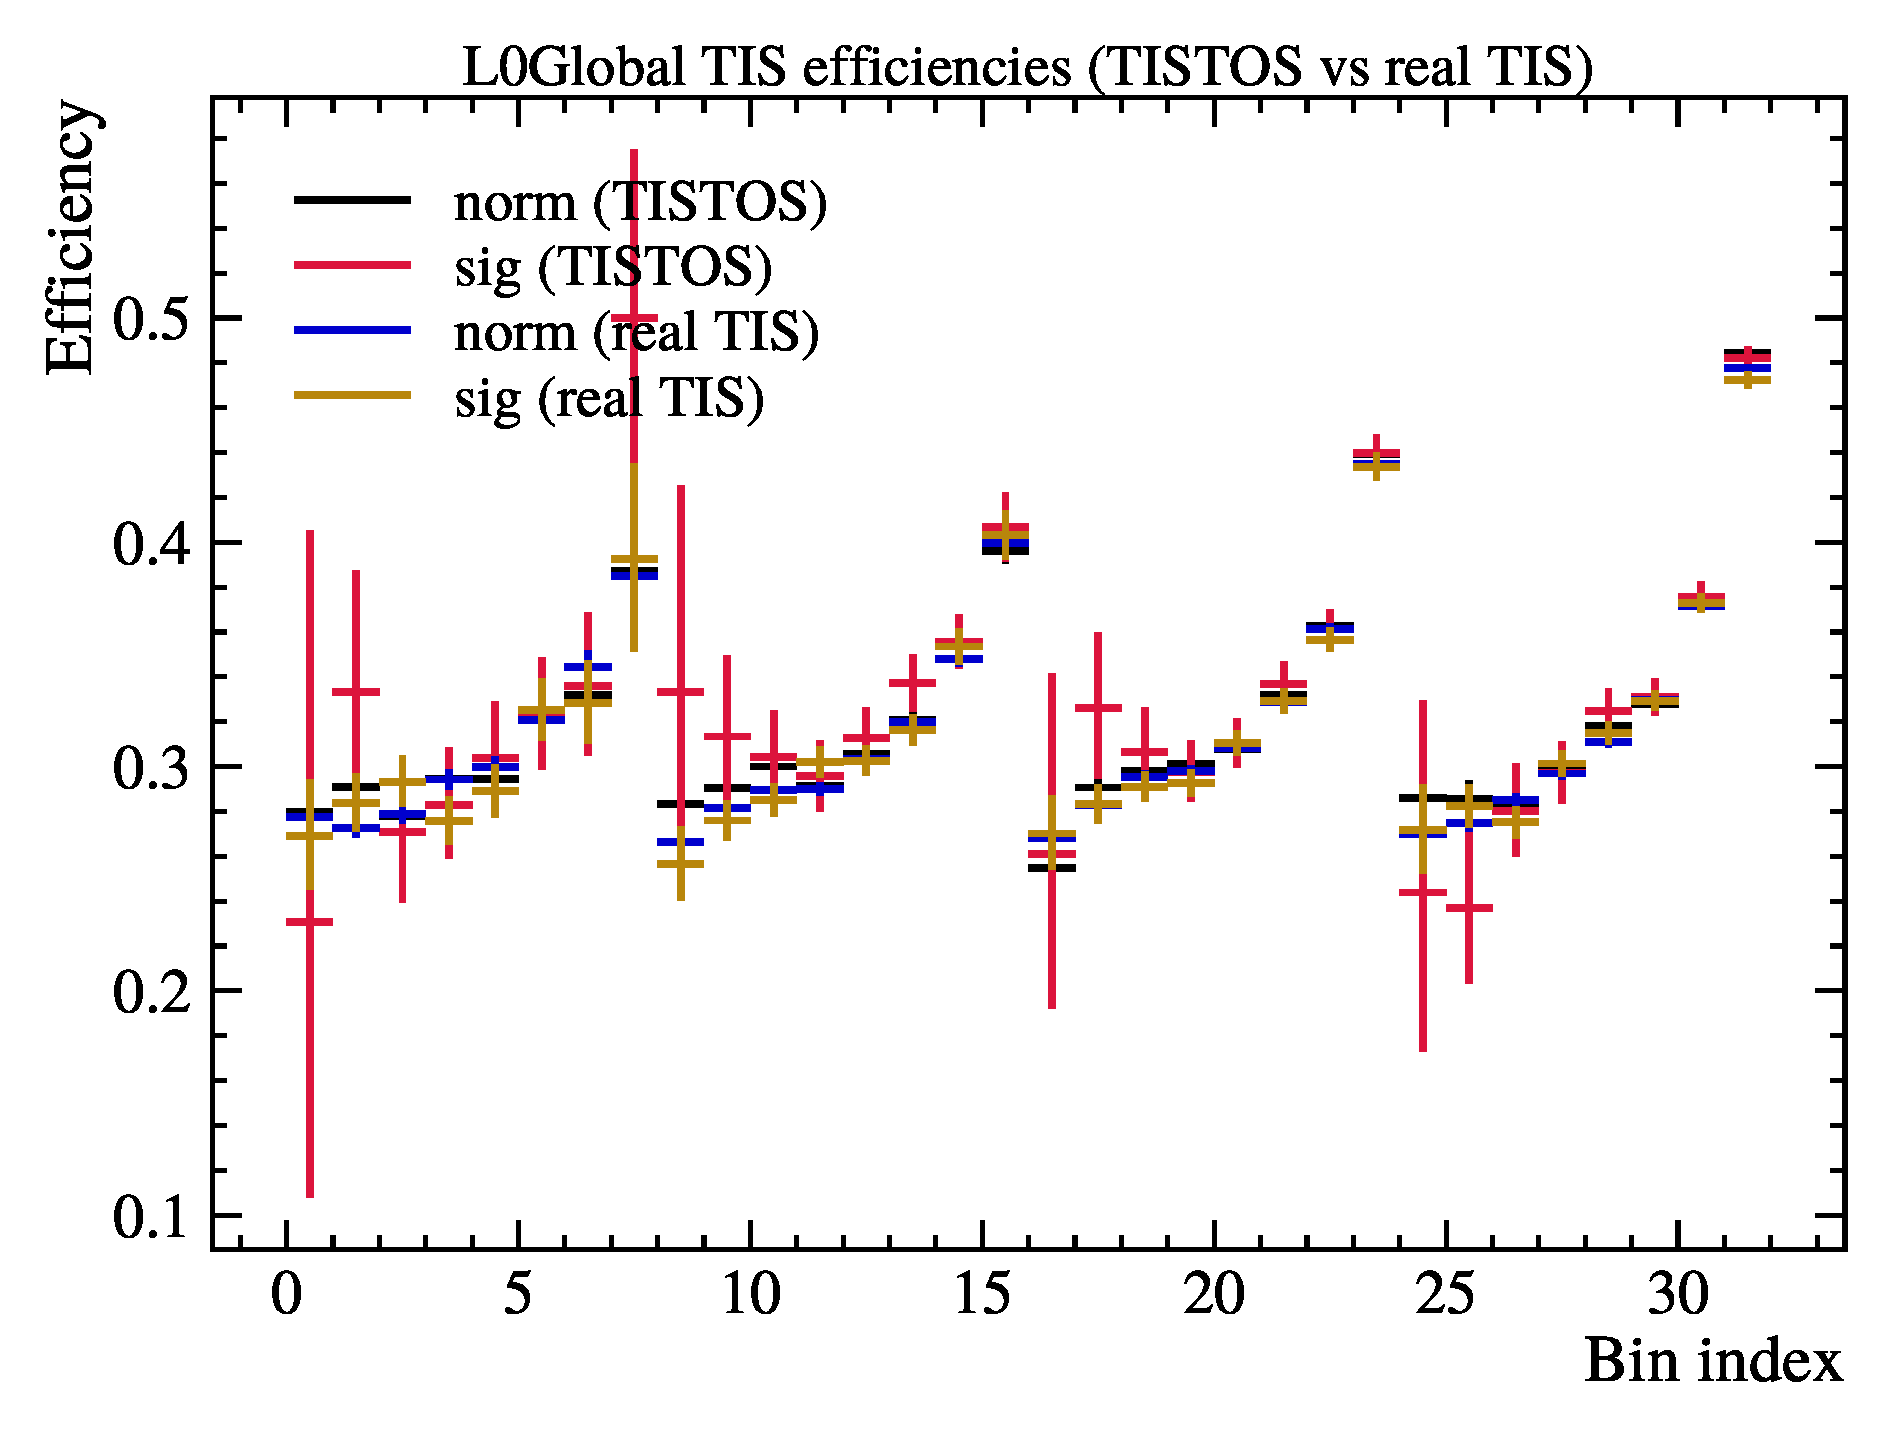
\includegraphics[width=0.32\textwidth]{
        ./figs-supplemental-plots/l0global-tis/l0_global_tis_eff_bin_idx_comp.pdf
    }
    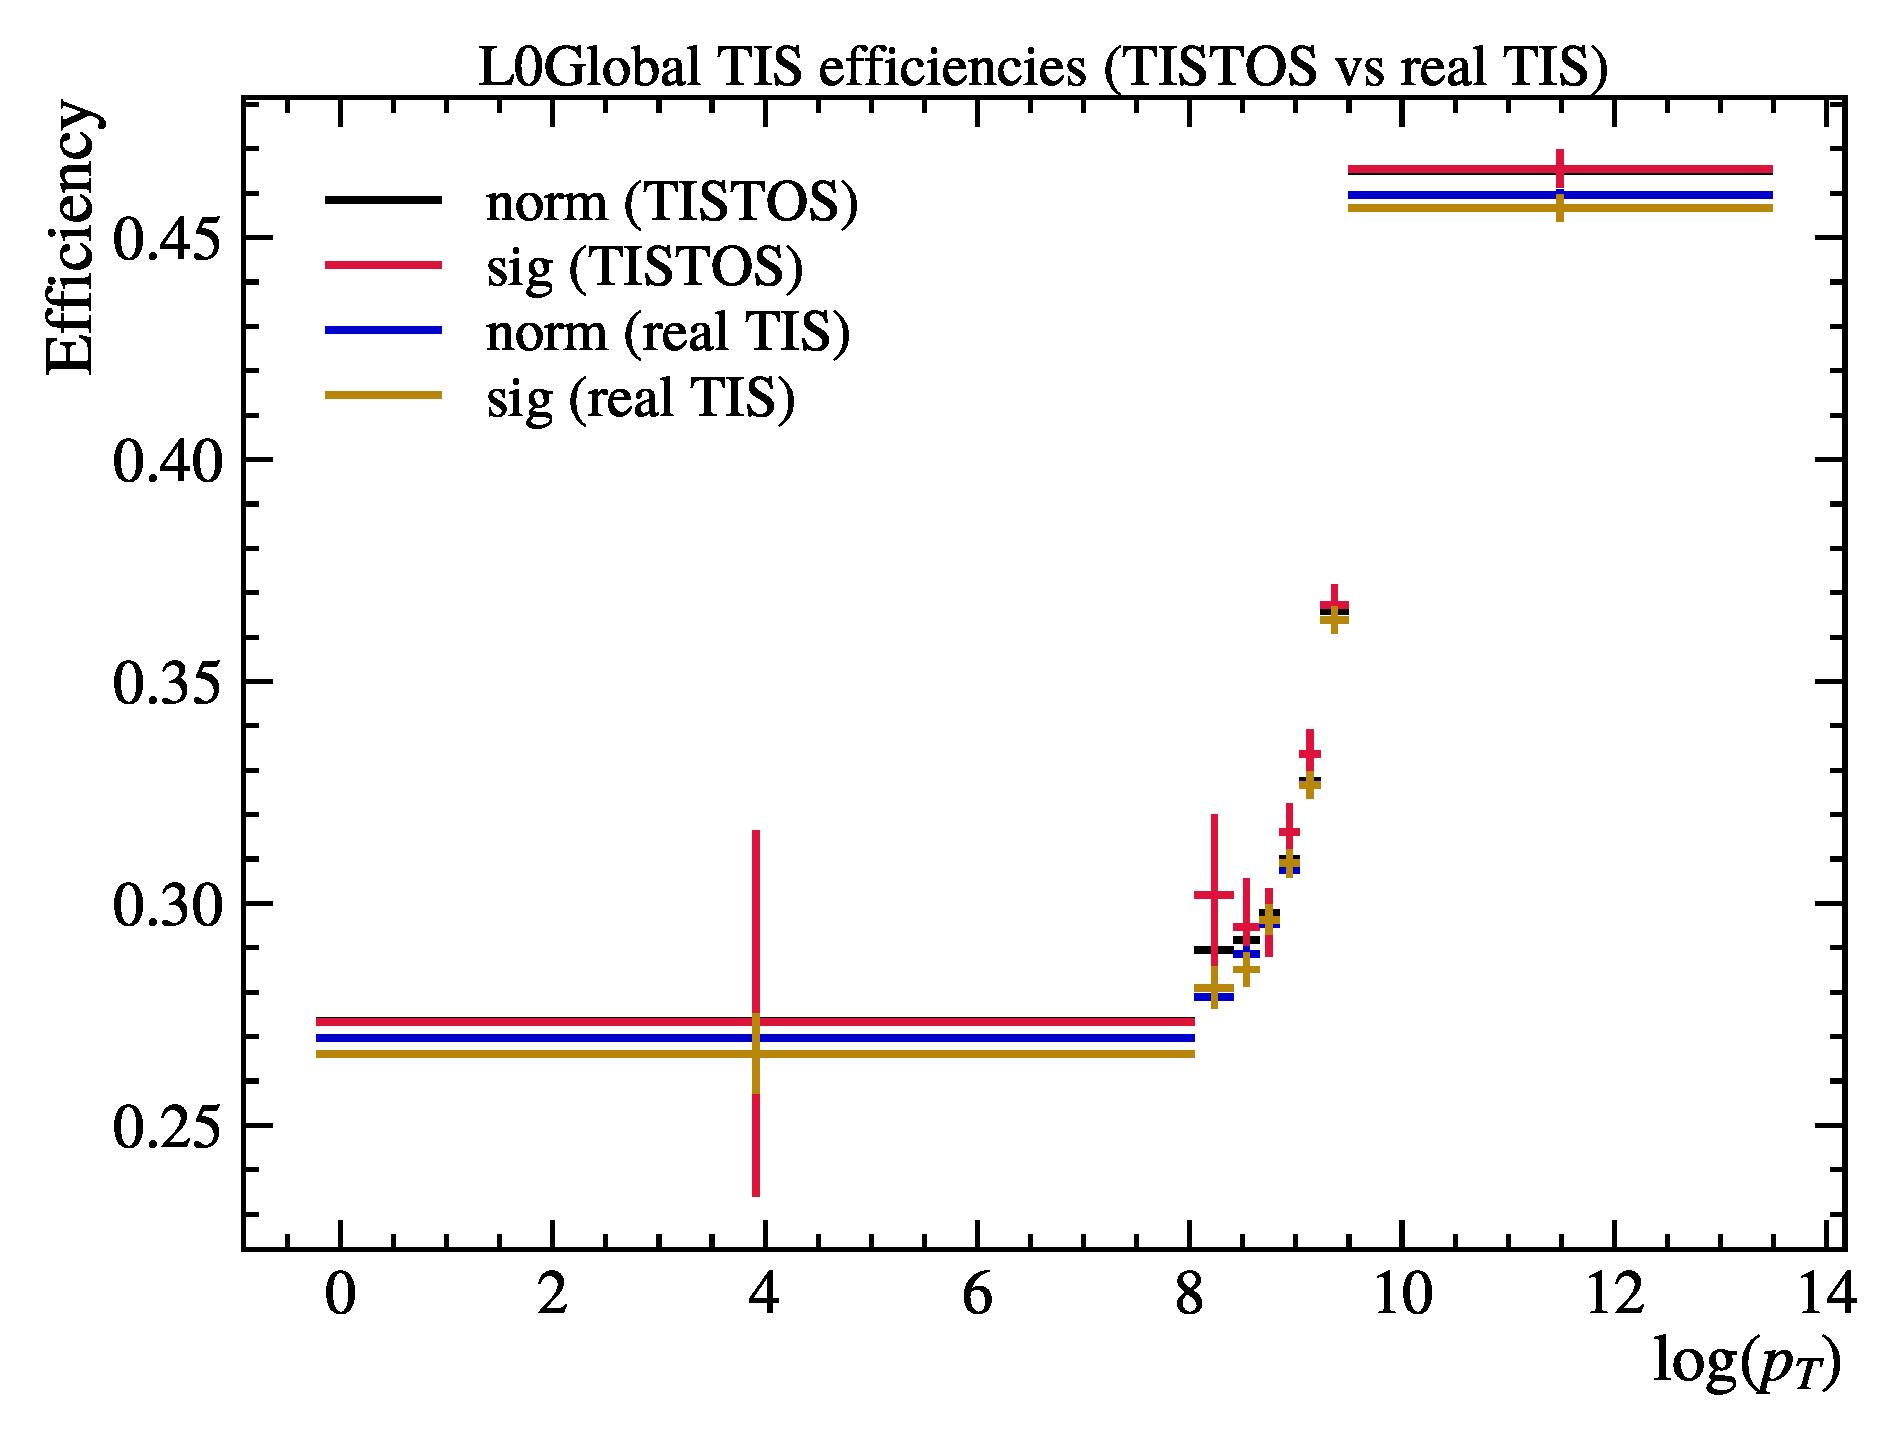
\includegraphics[width=0.32\textwidth]{
        ./figs-supplemental-plots/l0global-tis/l0_global_tis_eff_log_pt_comp.pdf
    }
    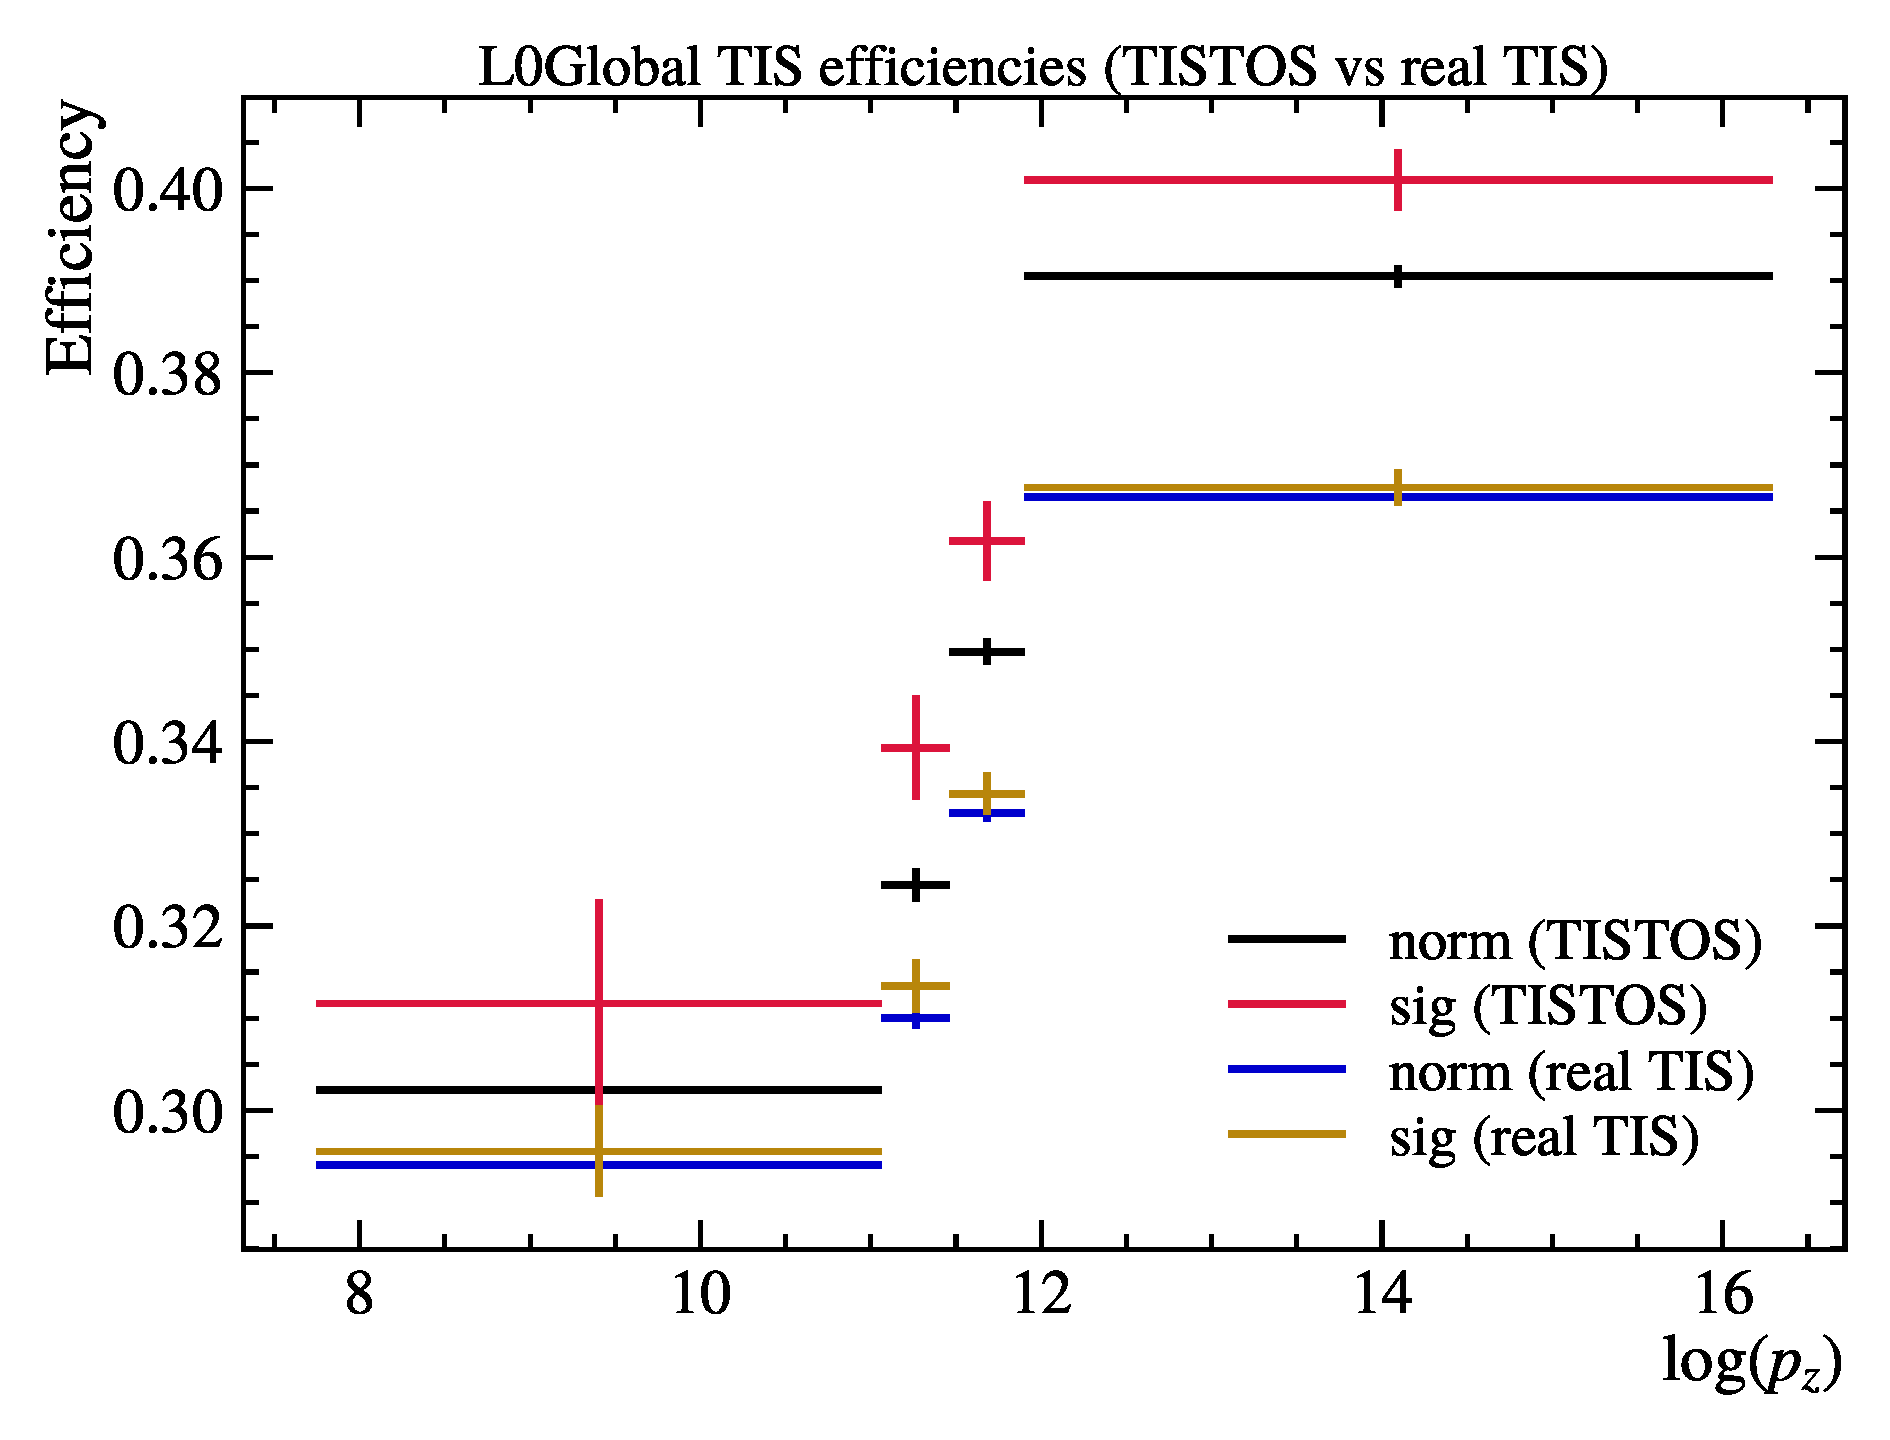
\includegraphics[width=0.32\textwidth]{
        ./figs-supplemental-plots/l0global-tis/l0_global_tis_eff_log_pz_comp.pdf
    }
    \caption[Check if TISTOS method works on our MC samples.]{
        Check if TISTOS method works on our MC samples.

        The $p_T$ and $p_z$ momenta are MC true momenta of the $B$ meson.
        Bin index represents the index from an unrolled 2D
        true-$p_T$-true-$p_z$ histogram.

        Efficiencies at high-$\log(p_T)$ regions do not agree.
        Thus, if TISTOS method is used, the conclusion that L0Global TIS
        is portable among MC modes cannot be drawn.
    }
    \label{fig:check-l0global-tis-with-tistos}
\end{figure}


\section{Initial fit results for post-fit cocktail generation}
\label{appx:suppl:init-fit-cocktail}

The pre-control fit (step-1) results for the generation of post-fit cocktail
are shown in \cref{fig:init-fit-pre-ctrl-d0,fig:init-fit-pre-ctrl-dst};
the control fit (step-2) results are in
\cref{fig:init-fit-ctrl-d0,fig:init-fit-ctrl-dst};
the signal fit (step-3) results are in
\cref{fig:init-fit-sig-d0,fig:init-fit-sig-dst}.

\begin{figure}[htb]
    \centering
    \begin{subfigure}{\textwidth}
        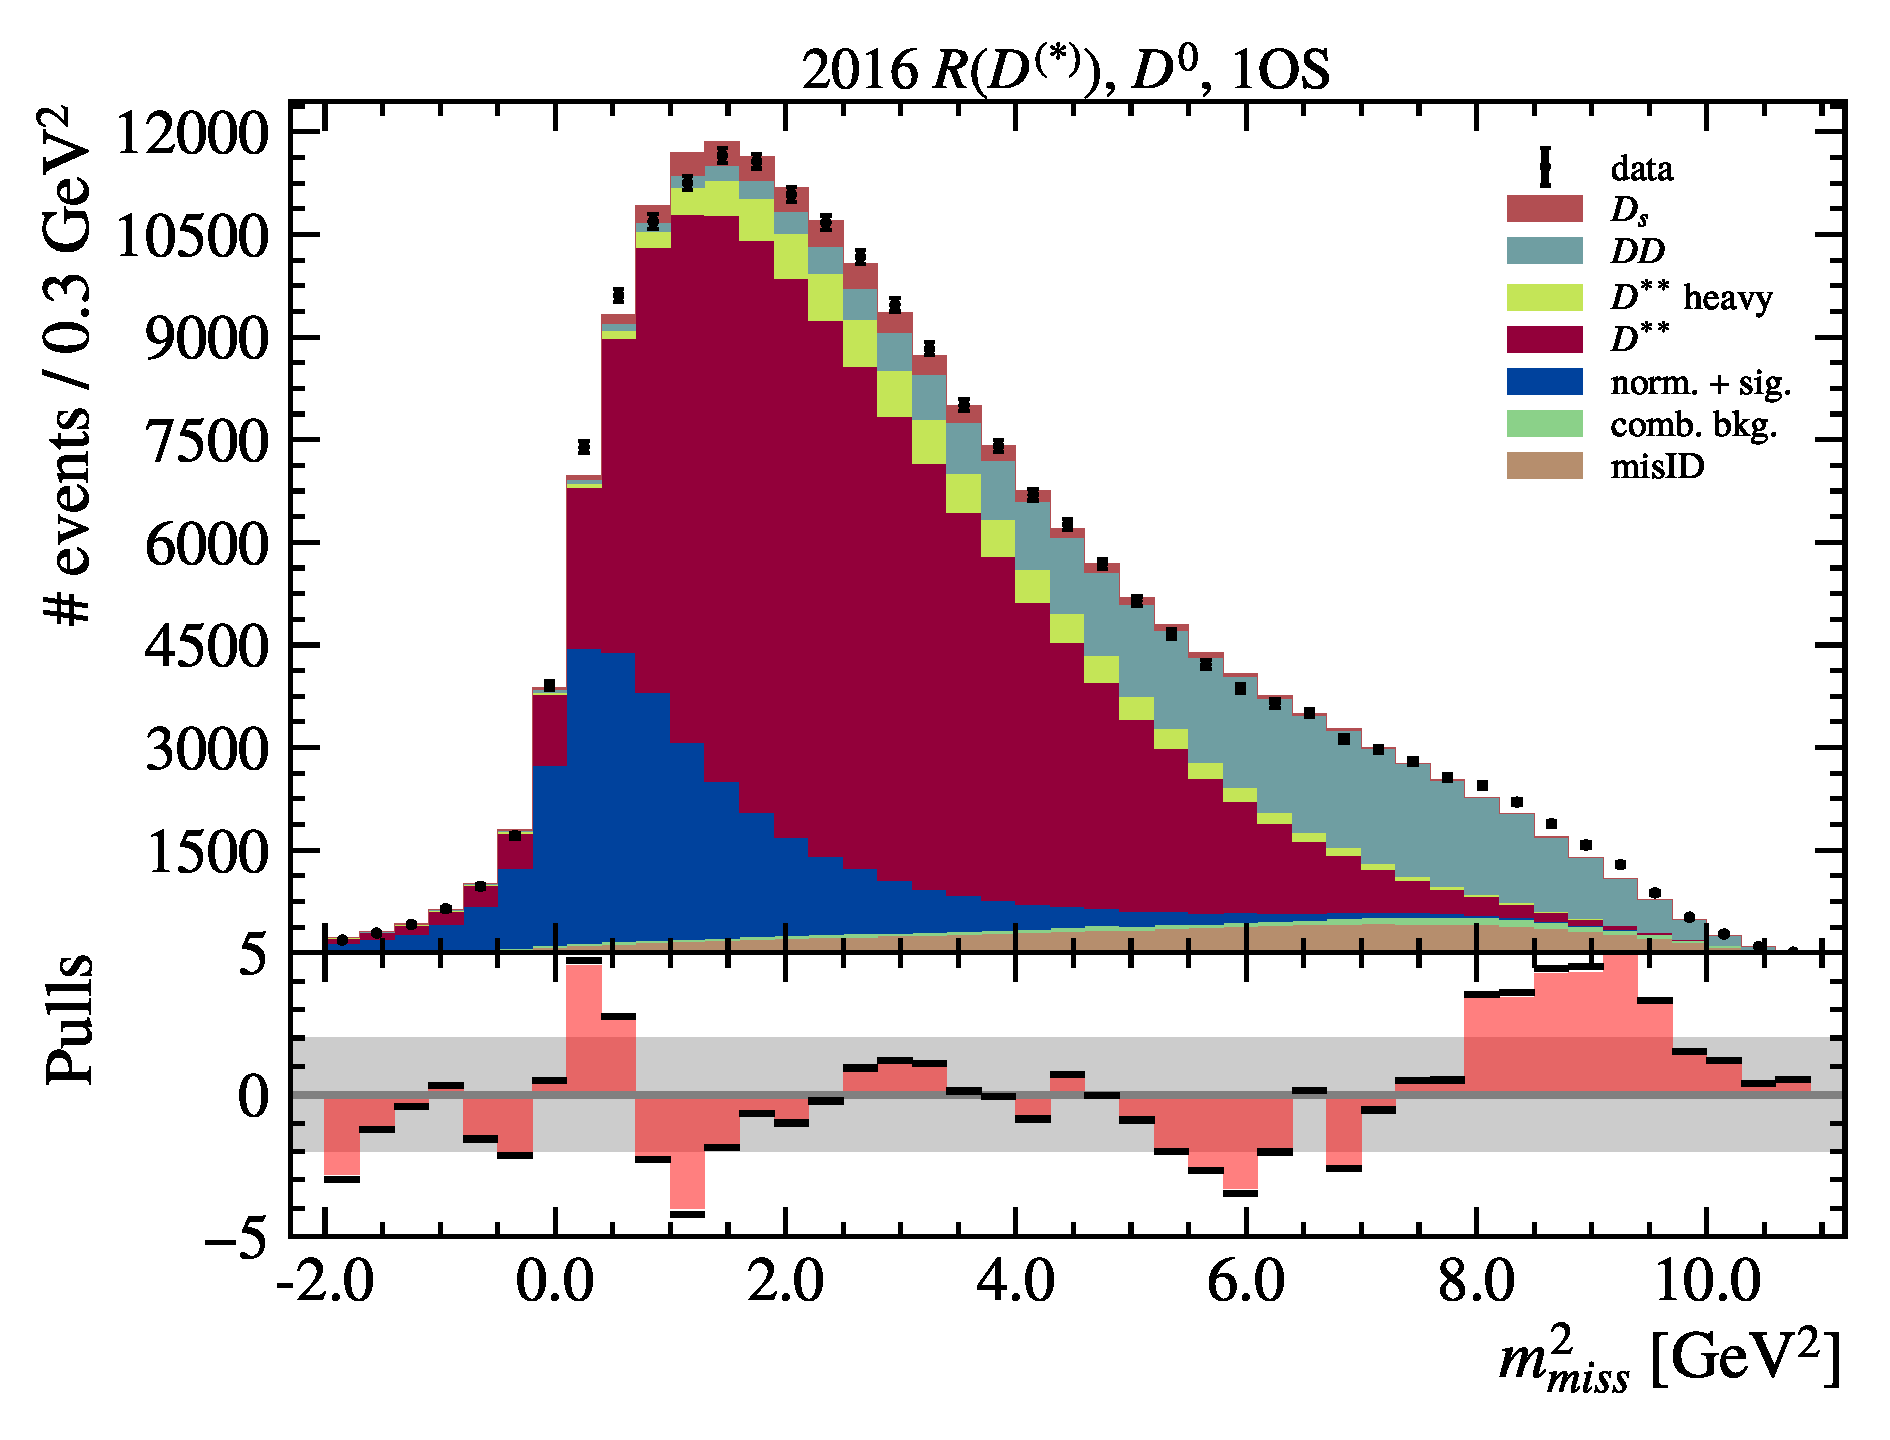
\includegraphics[width=0.32\textwidth]{./figs-supplemental-plots/init-fit/pre-ctrl/fit_result-stacked-D0-1os-mmiss2.pdf}
        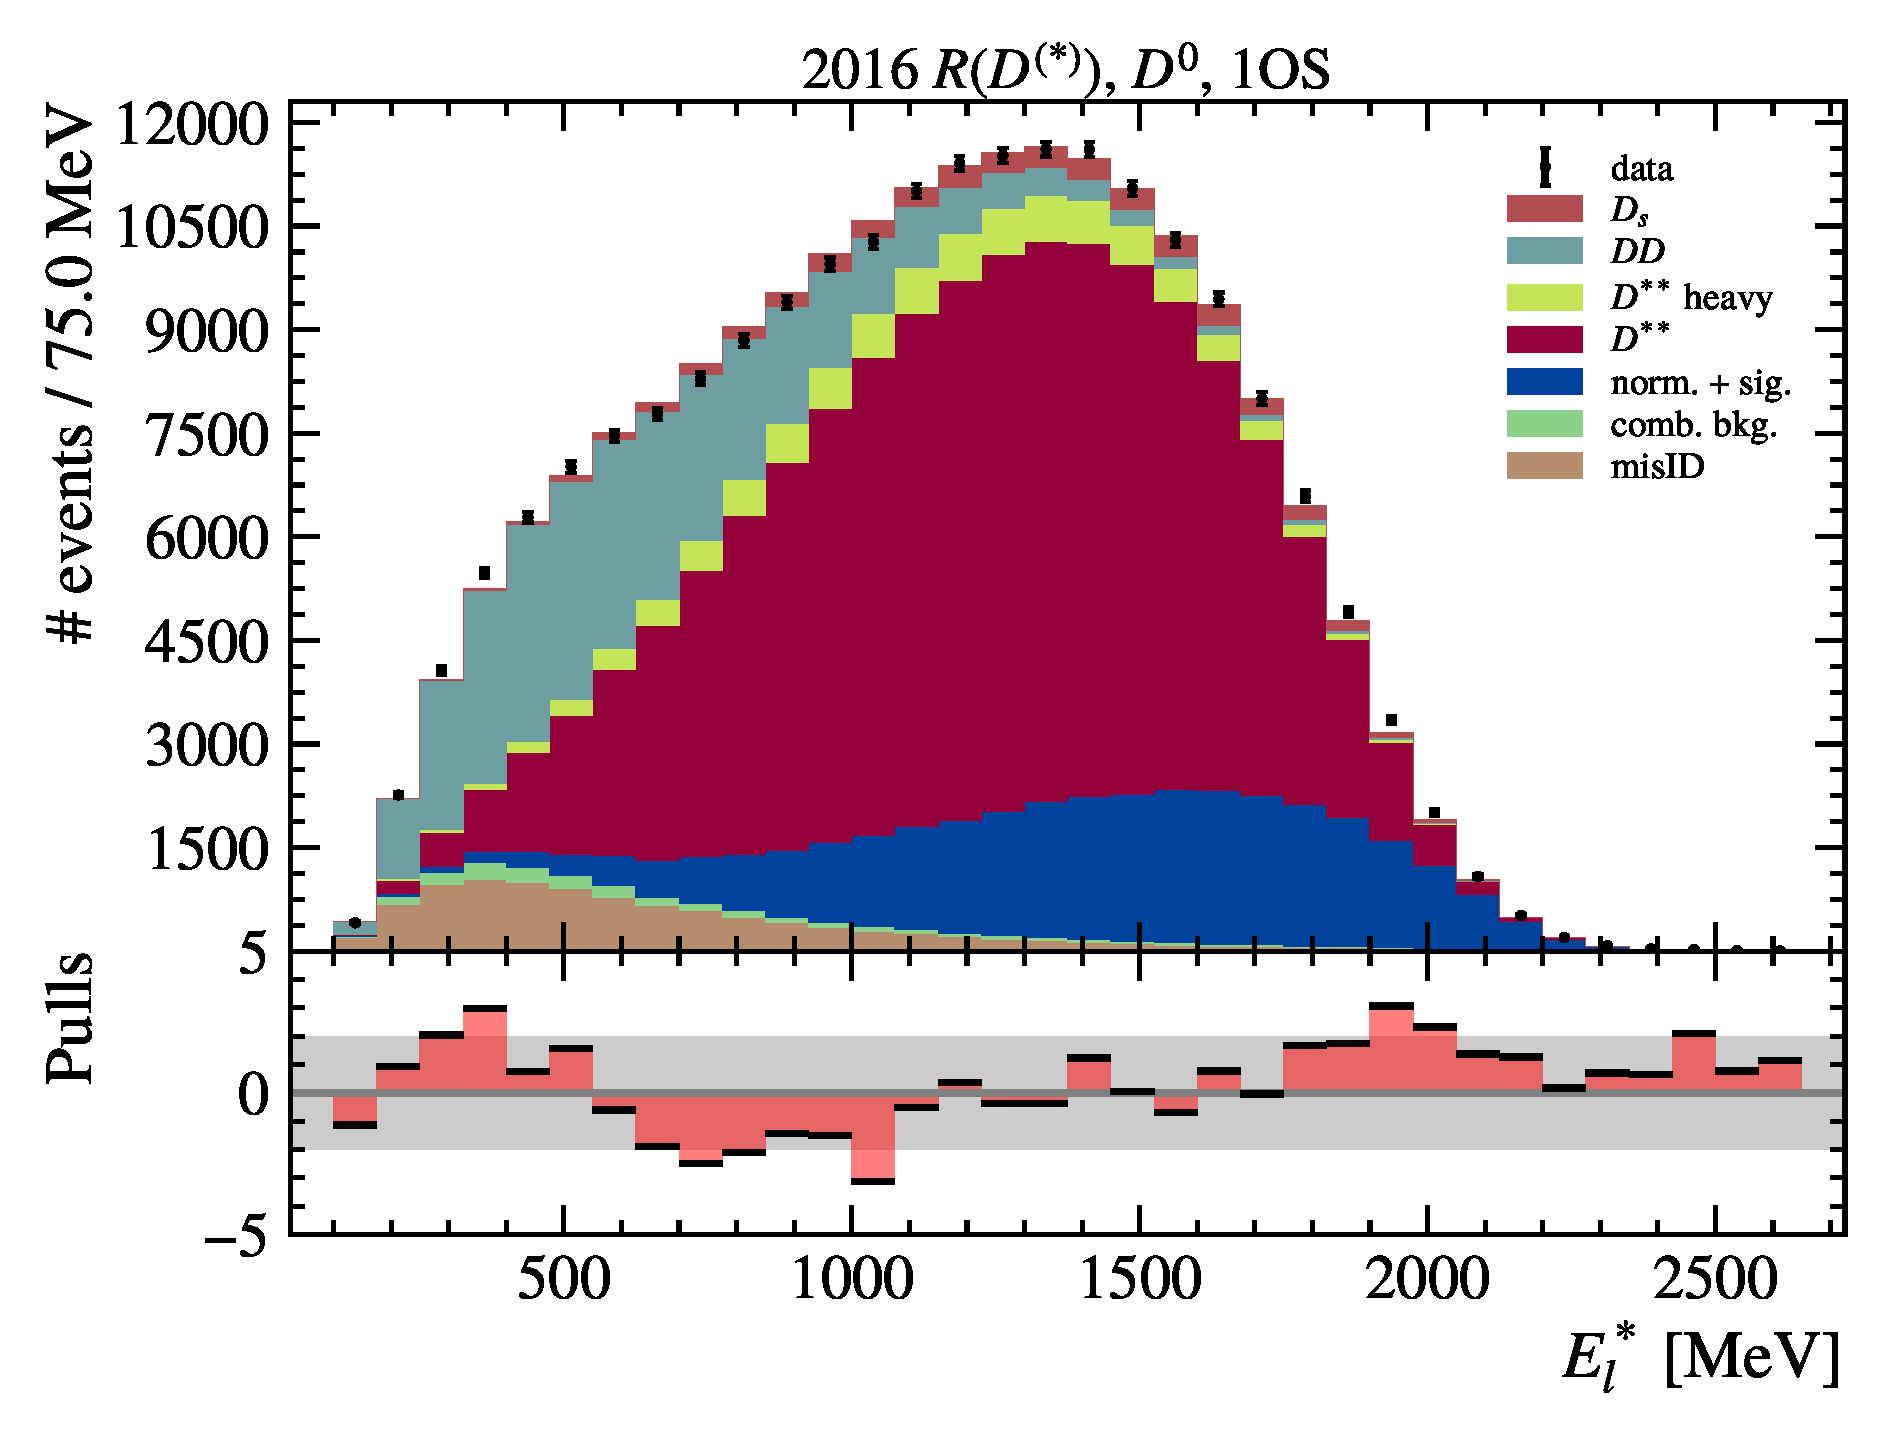
\includegraphics[width=0.32\textwidth]{./figs-supplemental-plots/init-fit/pre-ctrl/fit_result-stacked-D0-1os-el.pdf}
        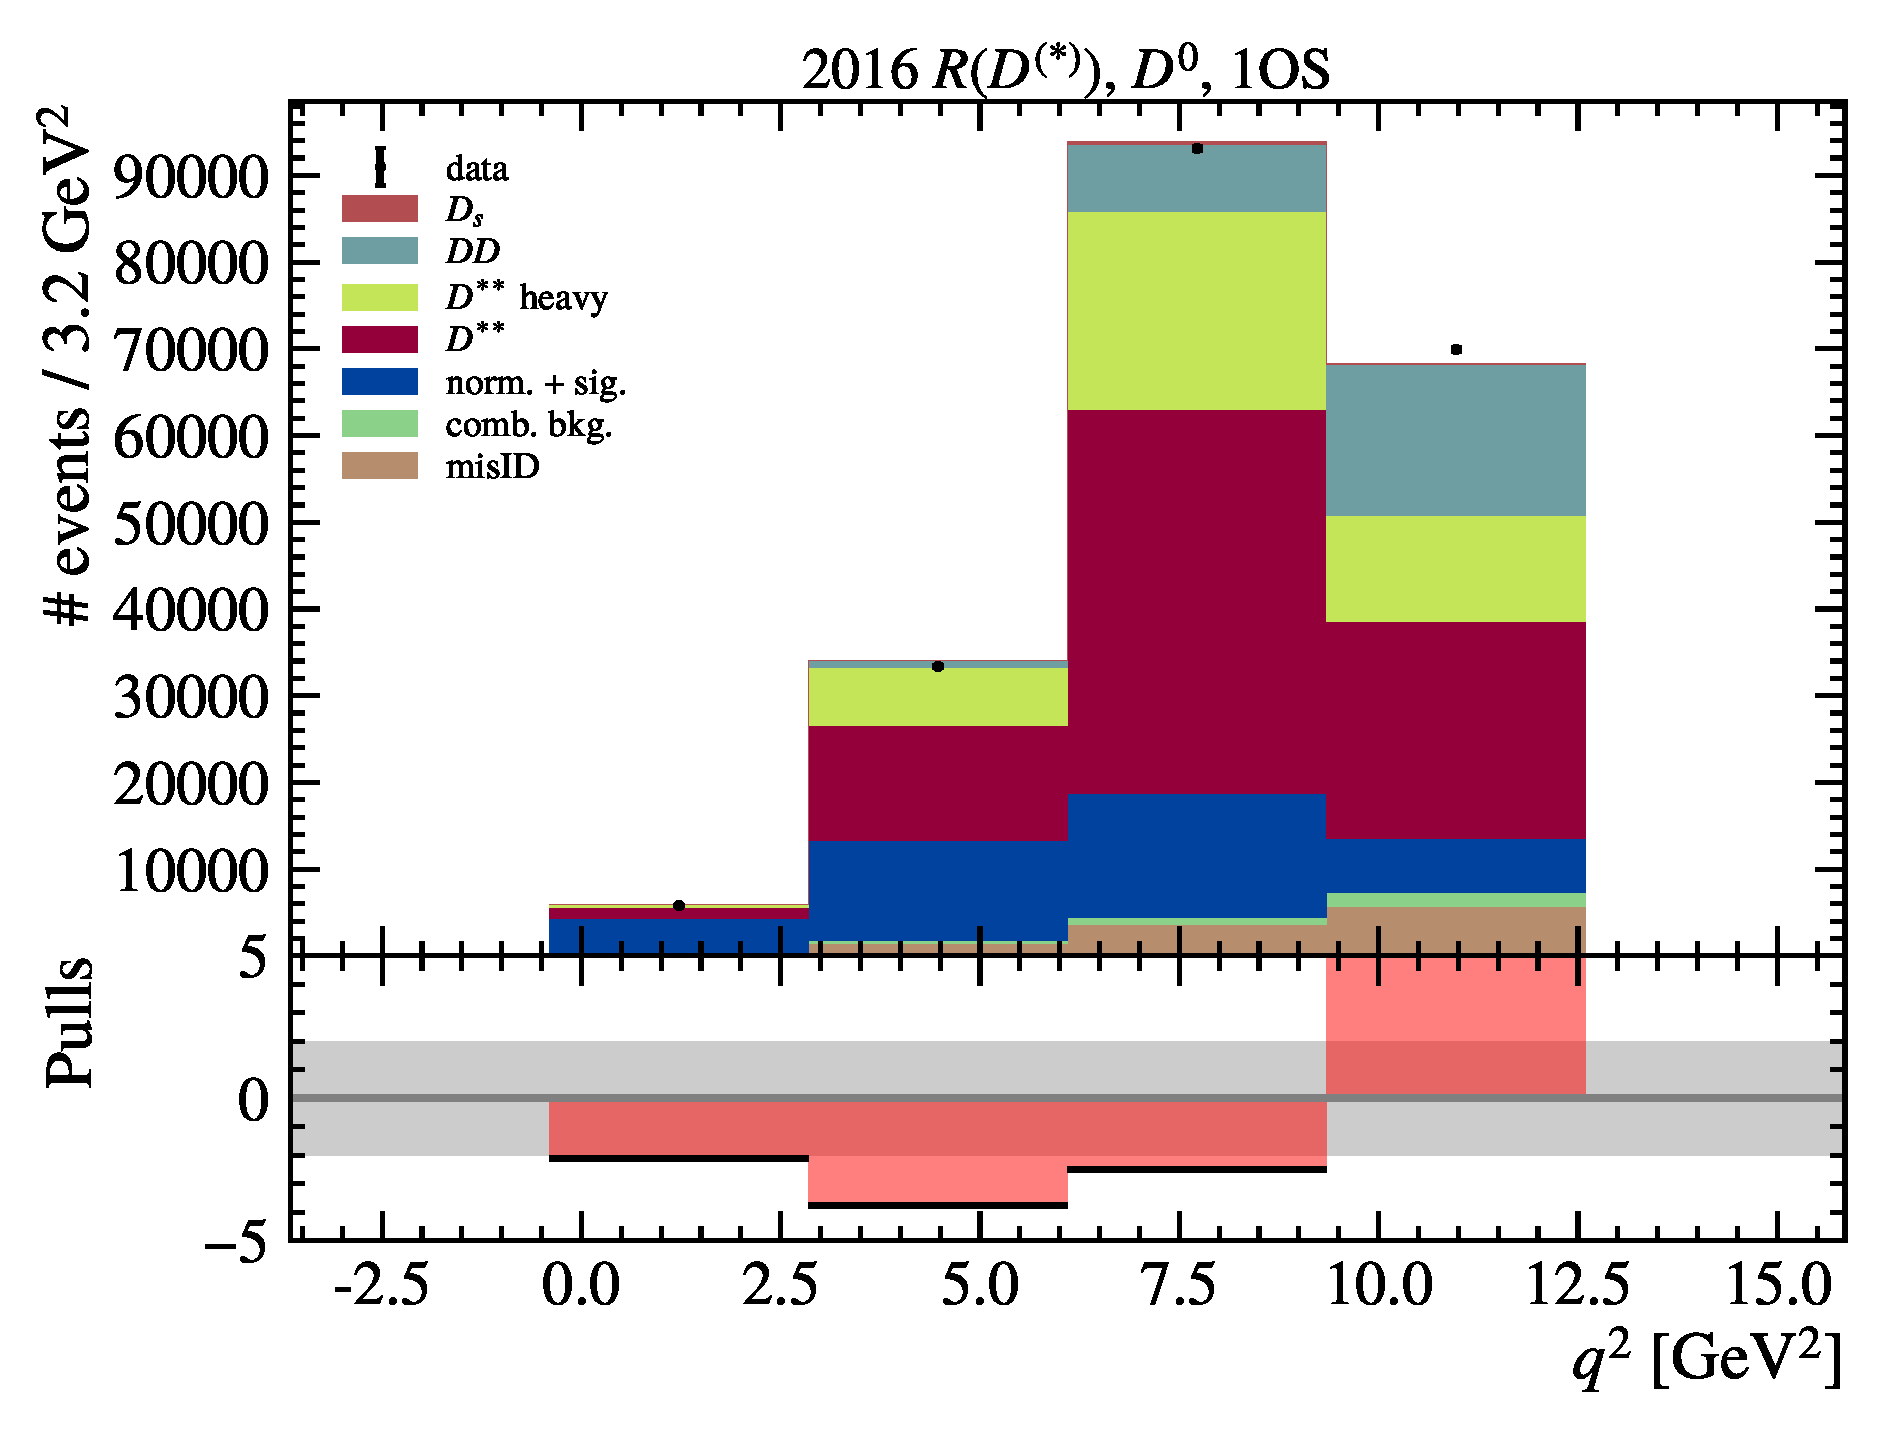
\includegraphics[width=0.32\textwidth]{./figs-supplemental-plots/init-fit/pre-ctrl/fit_result-stacked-D0-1os-q2.pdf}
        \caption{1OS}
    \end{subfigure}

    \begin{subfigure}{\textwidth}
        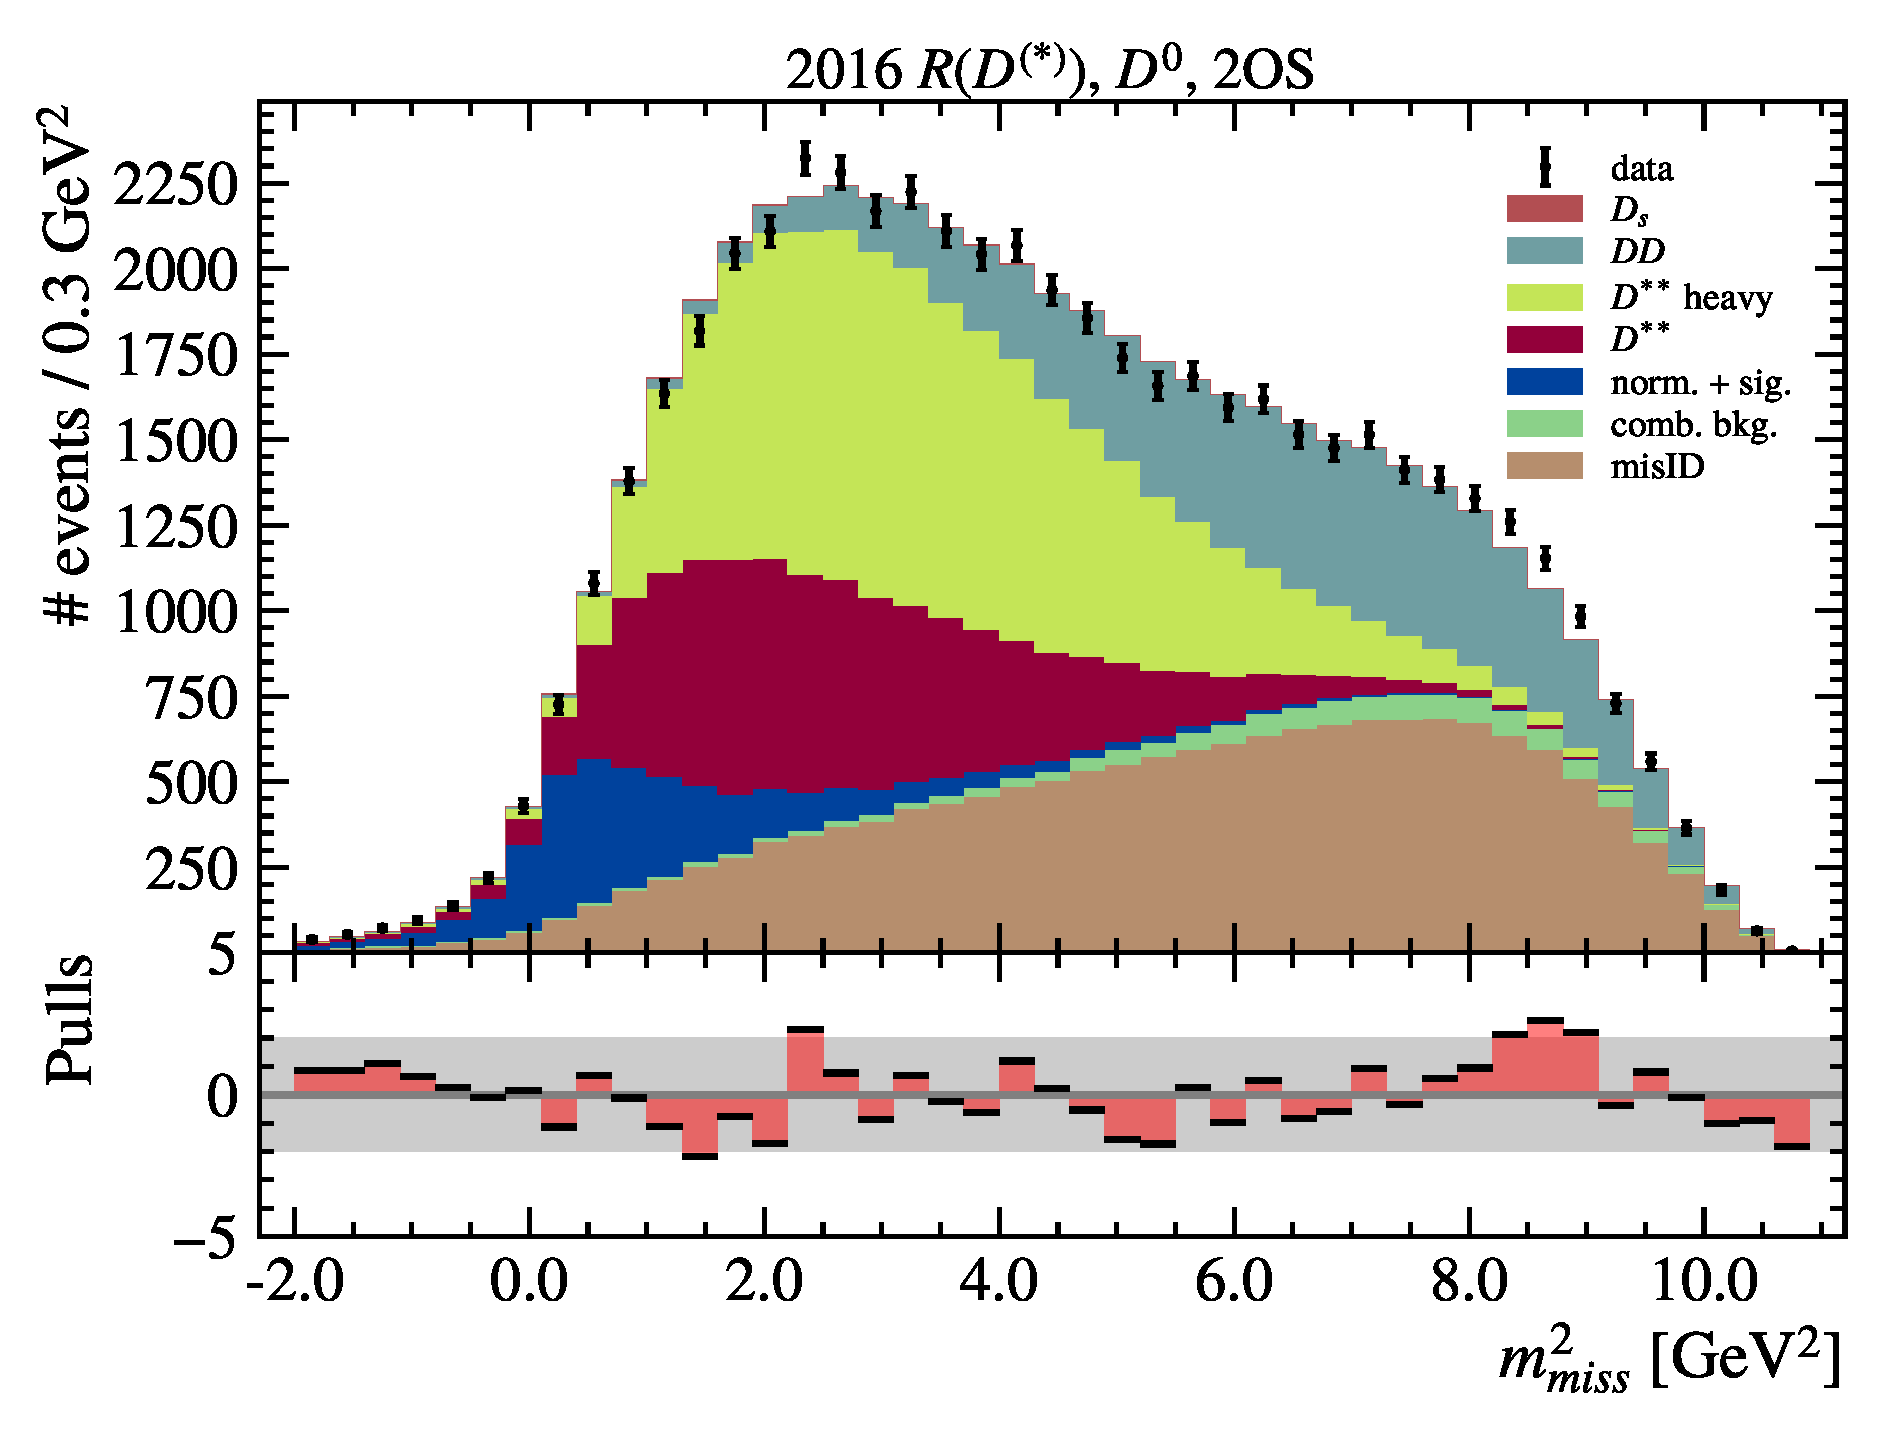
\includegraphics[width=0.32\textwidth]{./figs-supplemental-plots/init-fit/pre-ctrl/fit_result-stacked-D0-2os-mmiss2.pdf}
        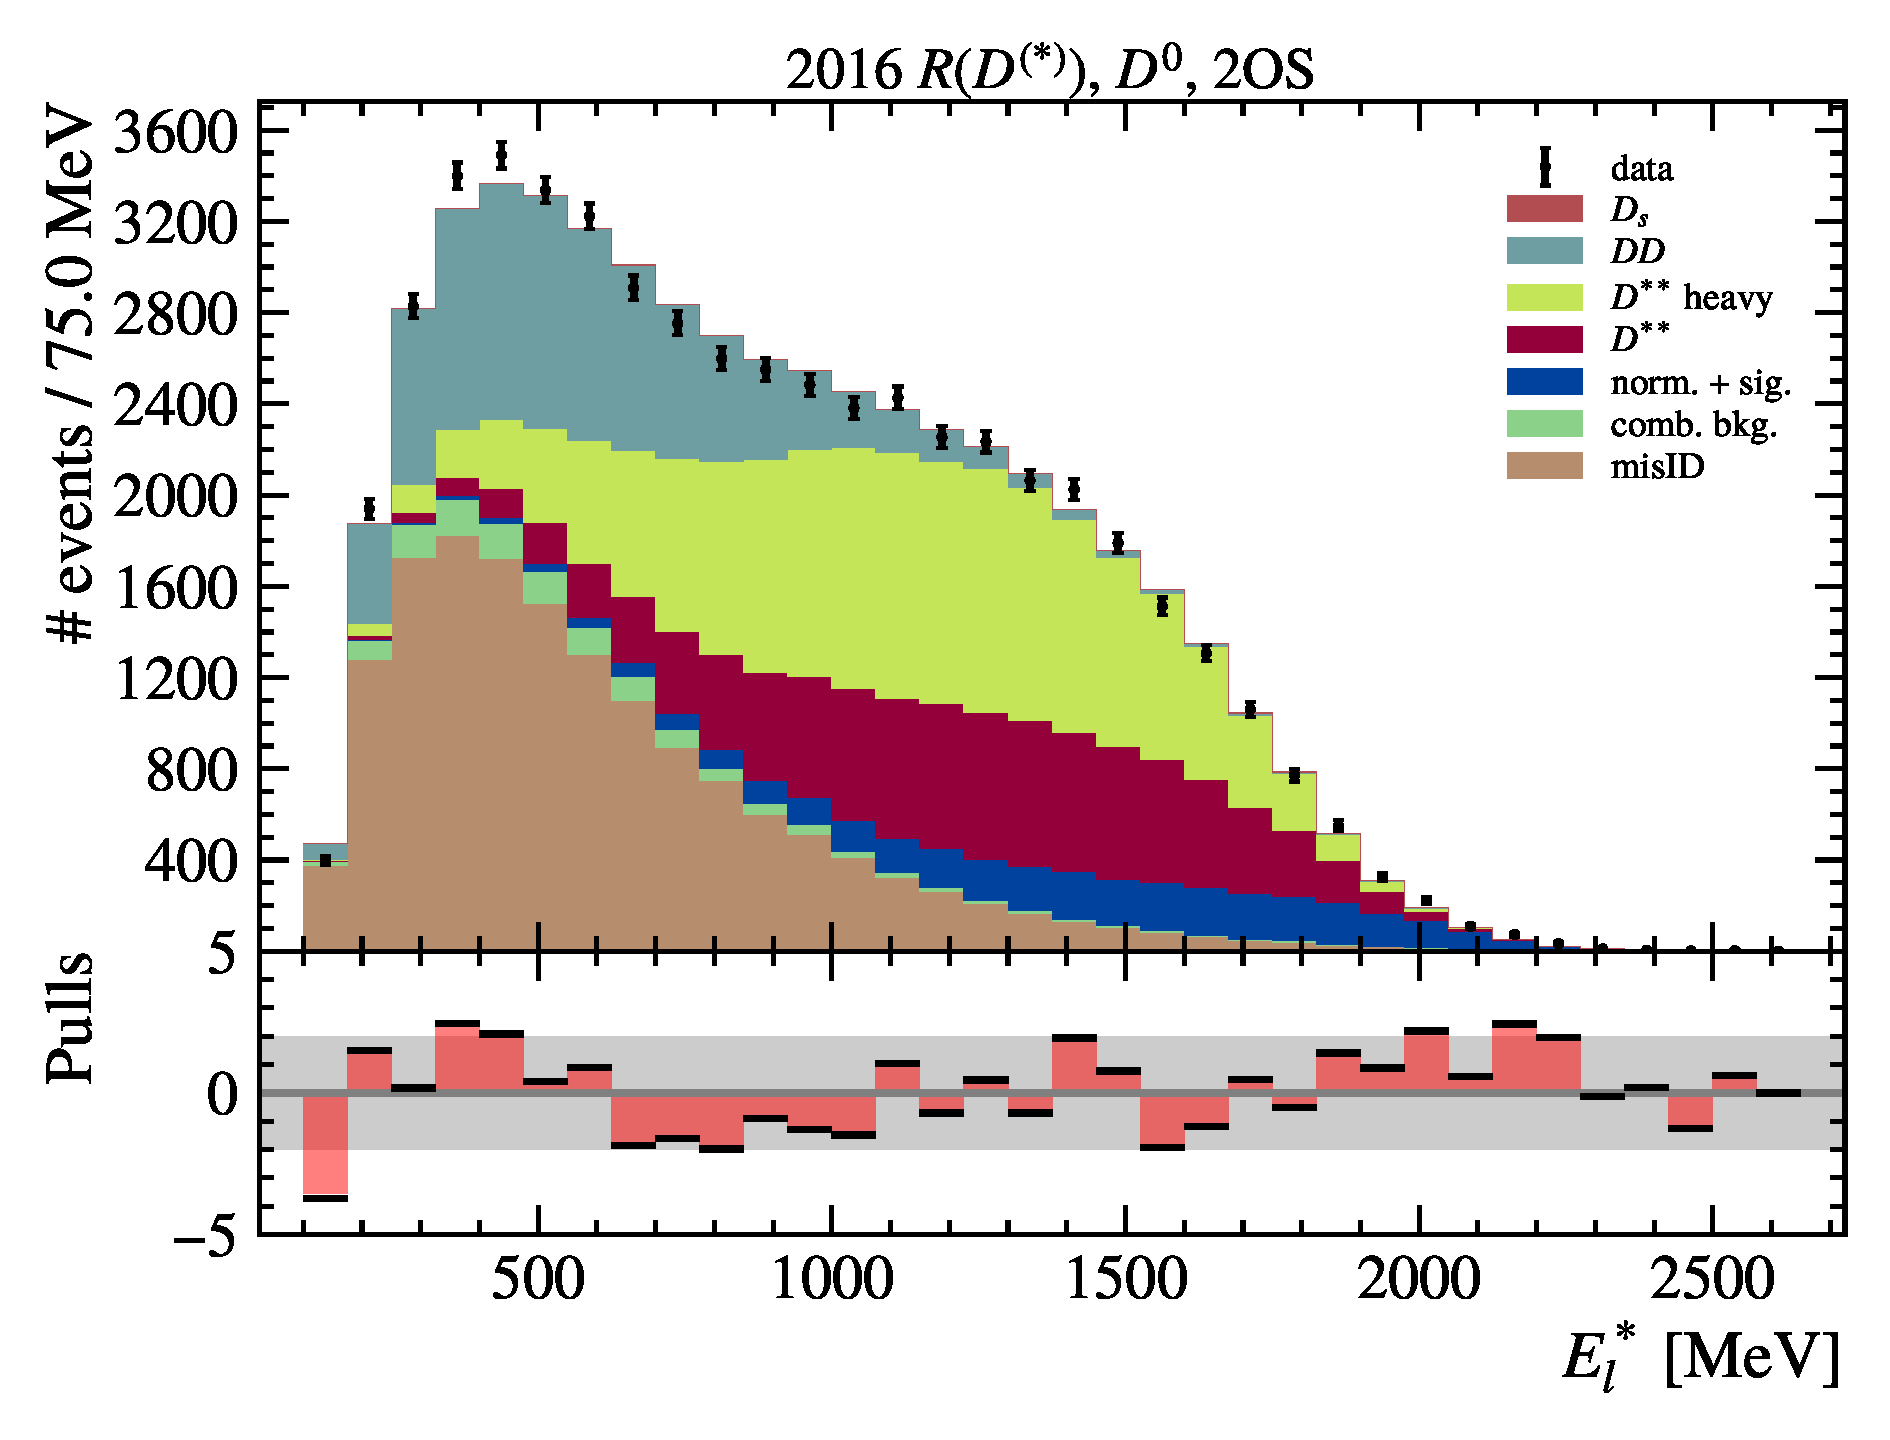
\includegraphics[width=0.32\textwidth]{./figs-supplemental-plots/init-fit/pre-ctrl/fit_result-stacked-D0-2os-el.pdf}
        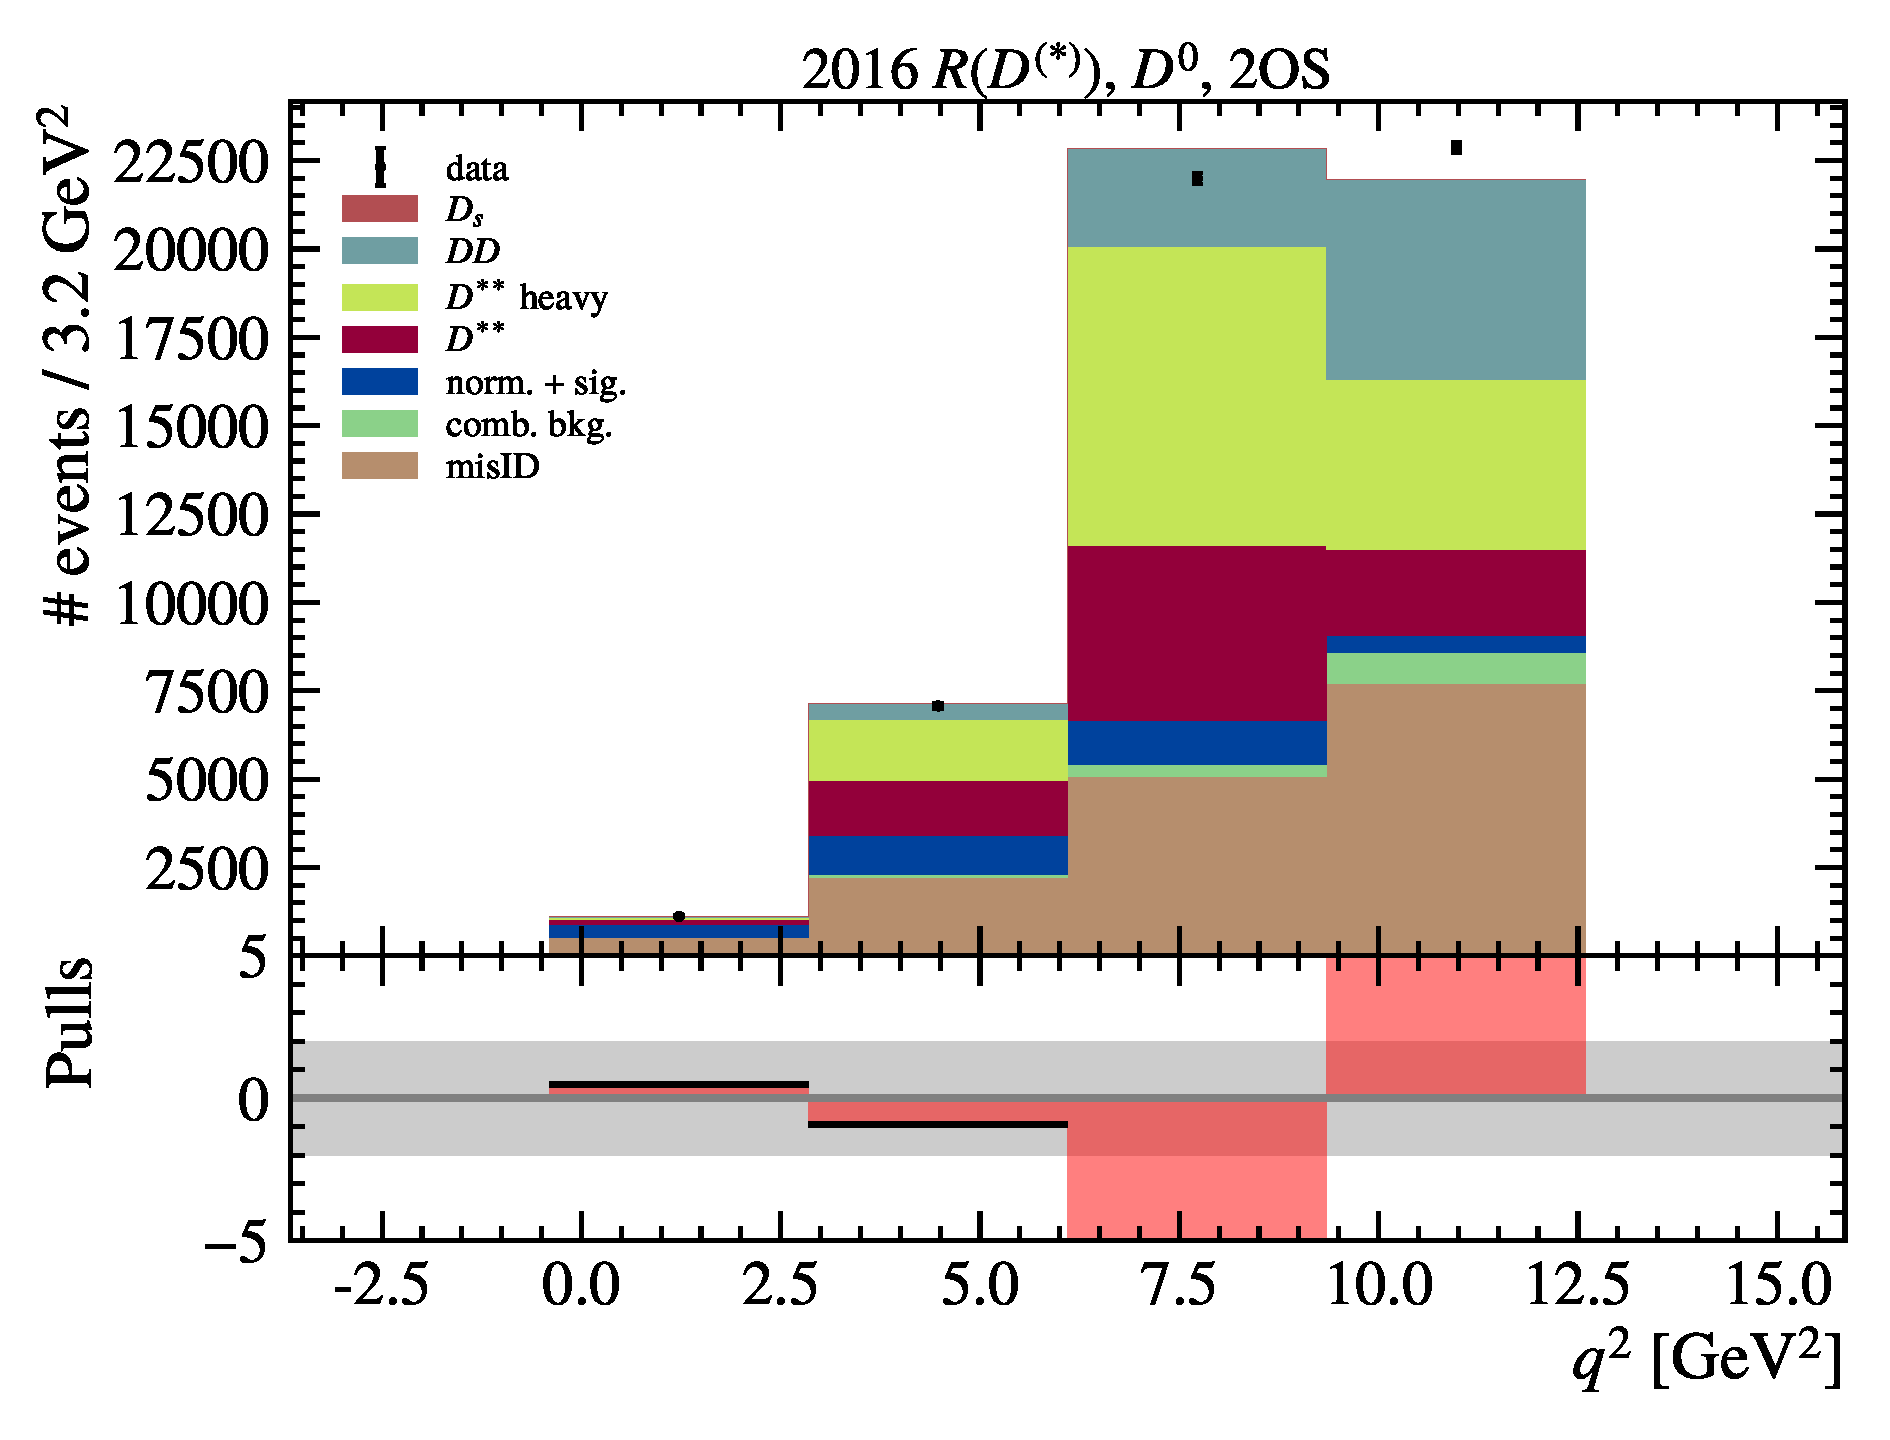
\includegraphics[width=0.32\textwidth]{./figs-supplemental-plots/init-fit/pre-ctrl/fit_result-stacked-D0-2os-q2.pdf}
        \caption{2OS}
    \end{subfigure}

    \begin{subfigure}{\textwidth}
        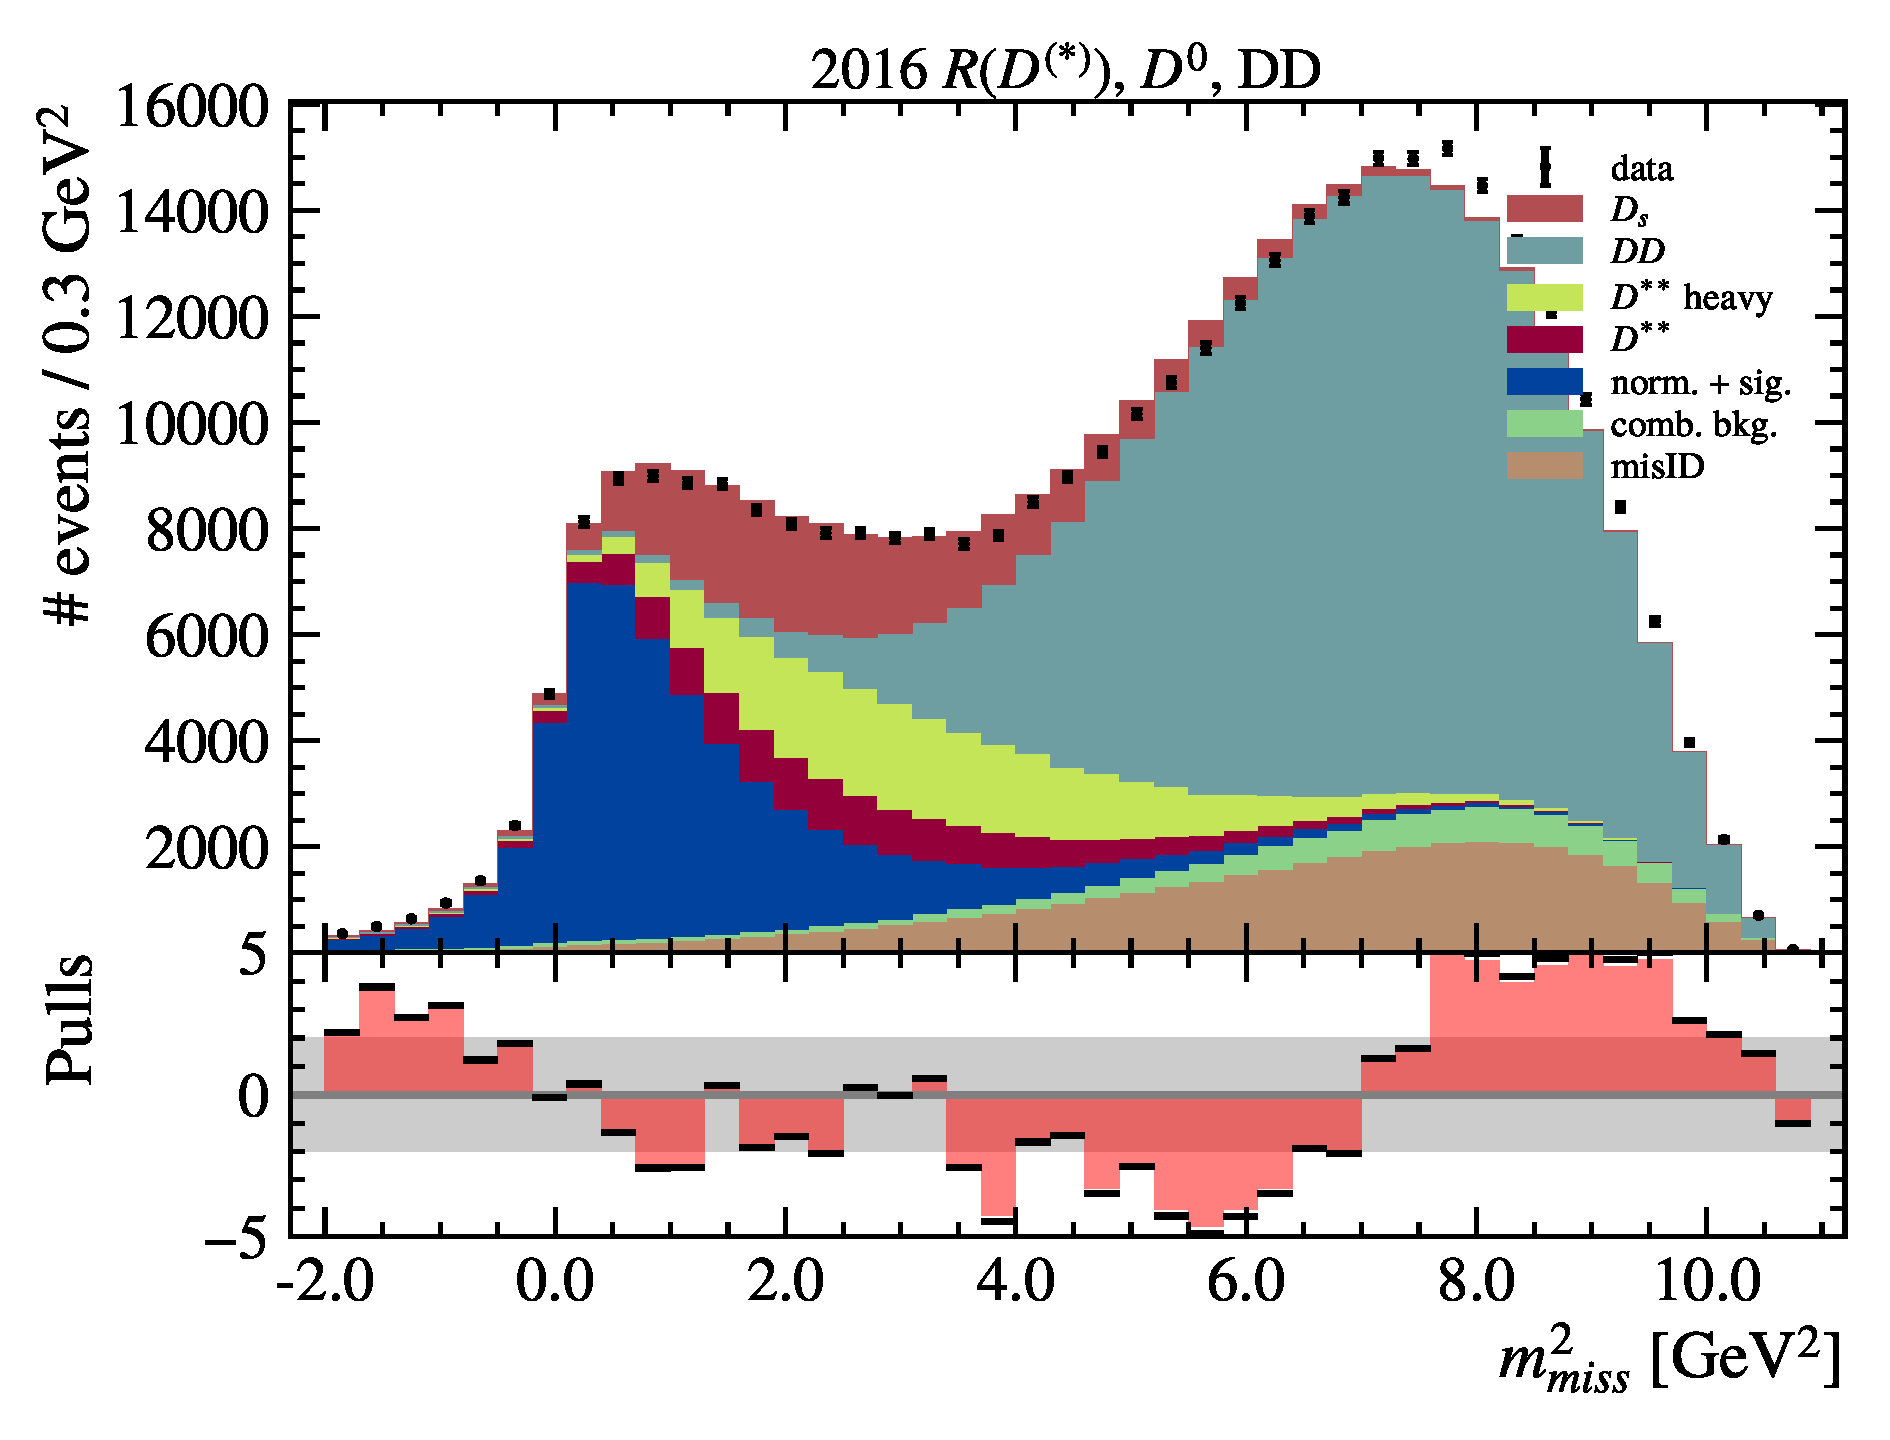
\includegraphics[width=0.32\textwidth]{./figs-supplemental-plots/init-fit/pre-ctrl/fit_result-stacked-D0-dd-mmiss2.pdf}
        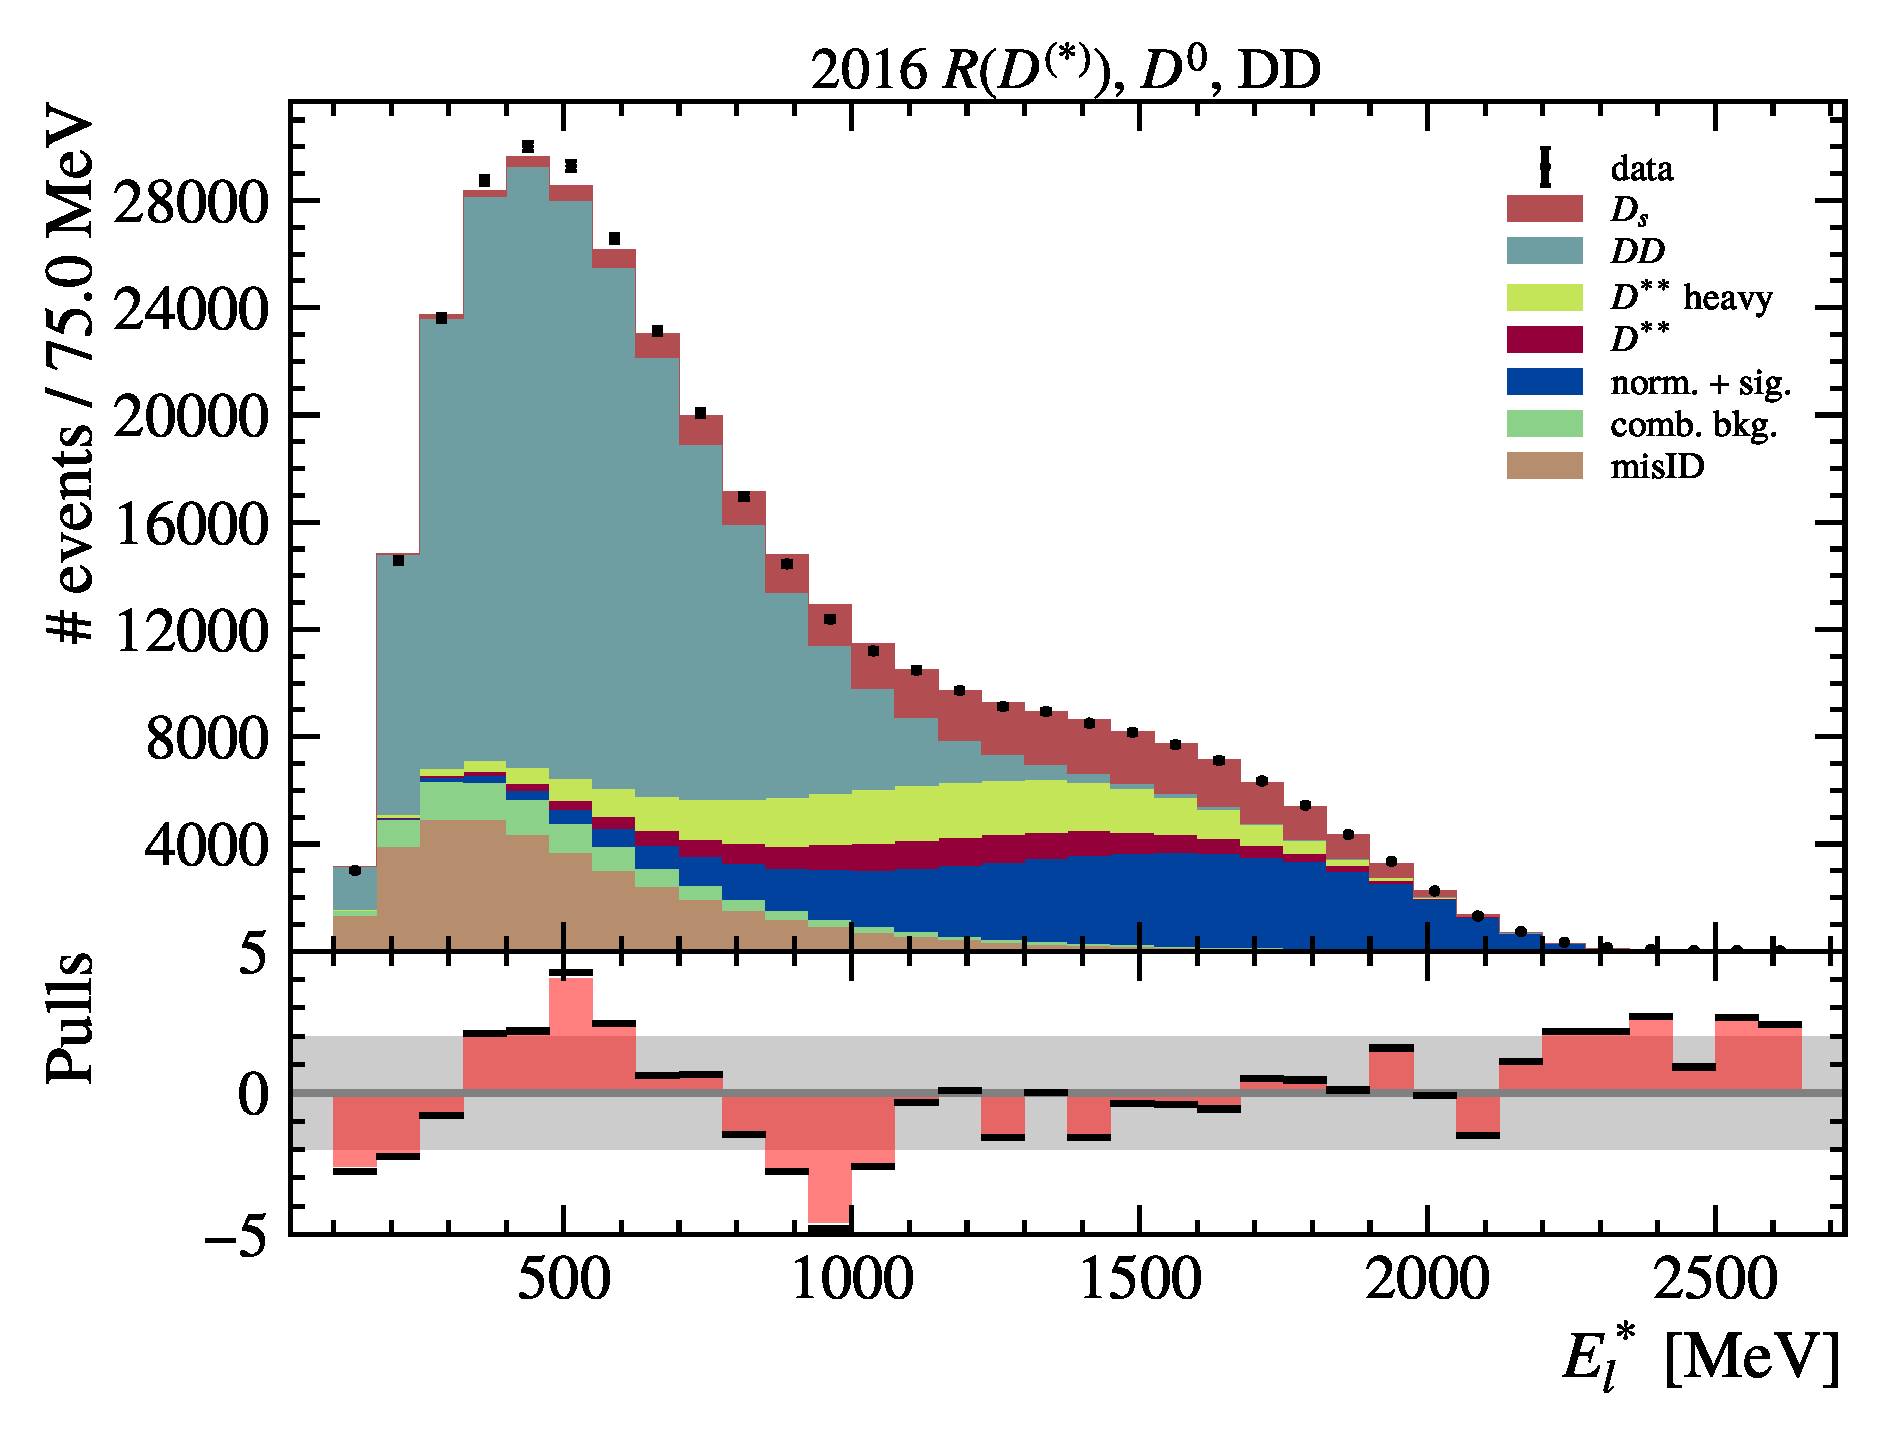
\includegraphics[width=0.32\textwidth]{./figs-supplemental-plots/init-fit/pre-ctrl/fit_result-stacked-D0-dd-el.pdf}
        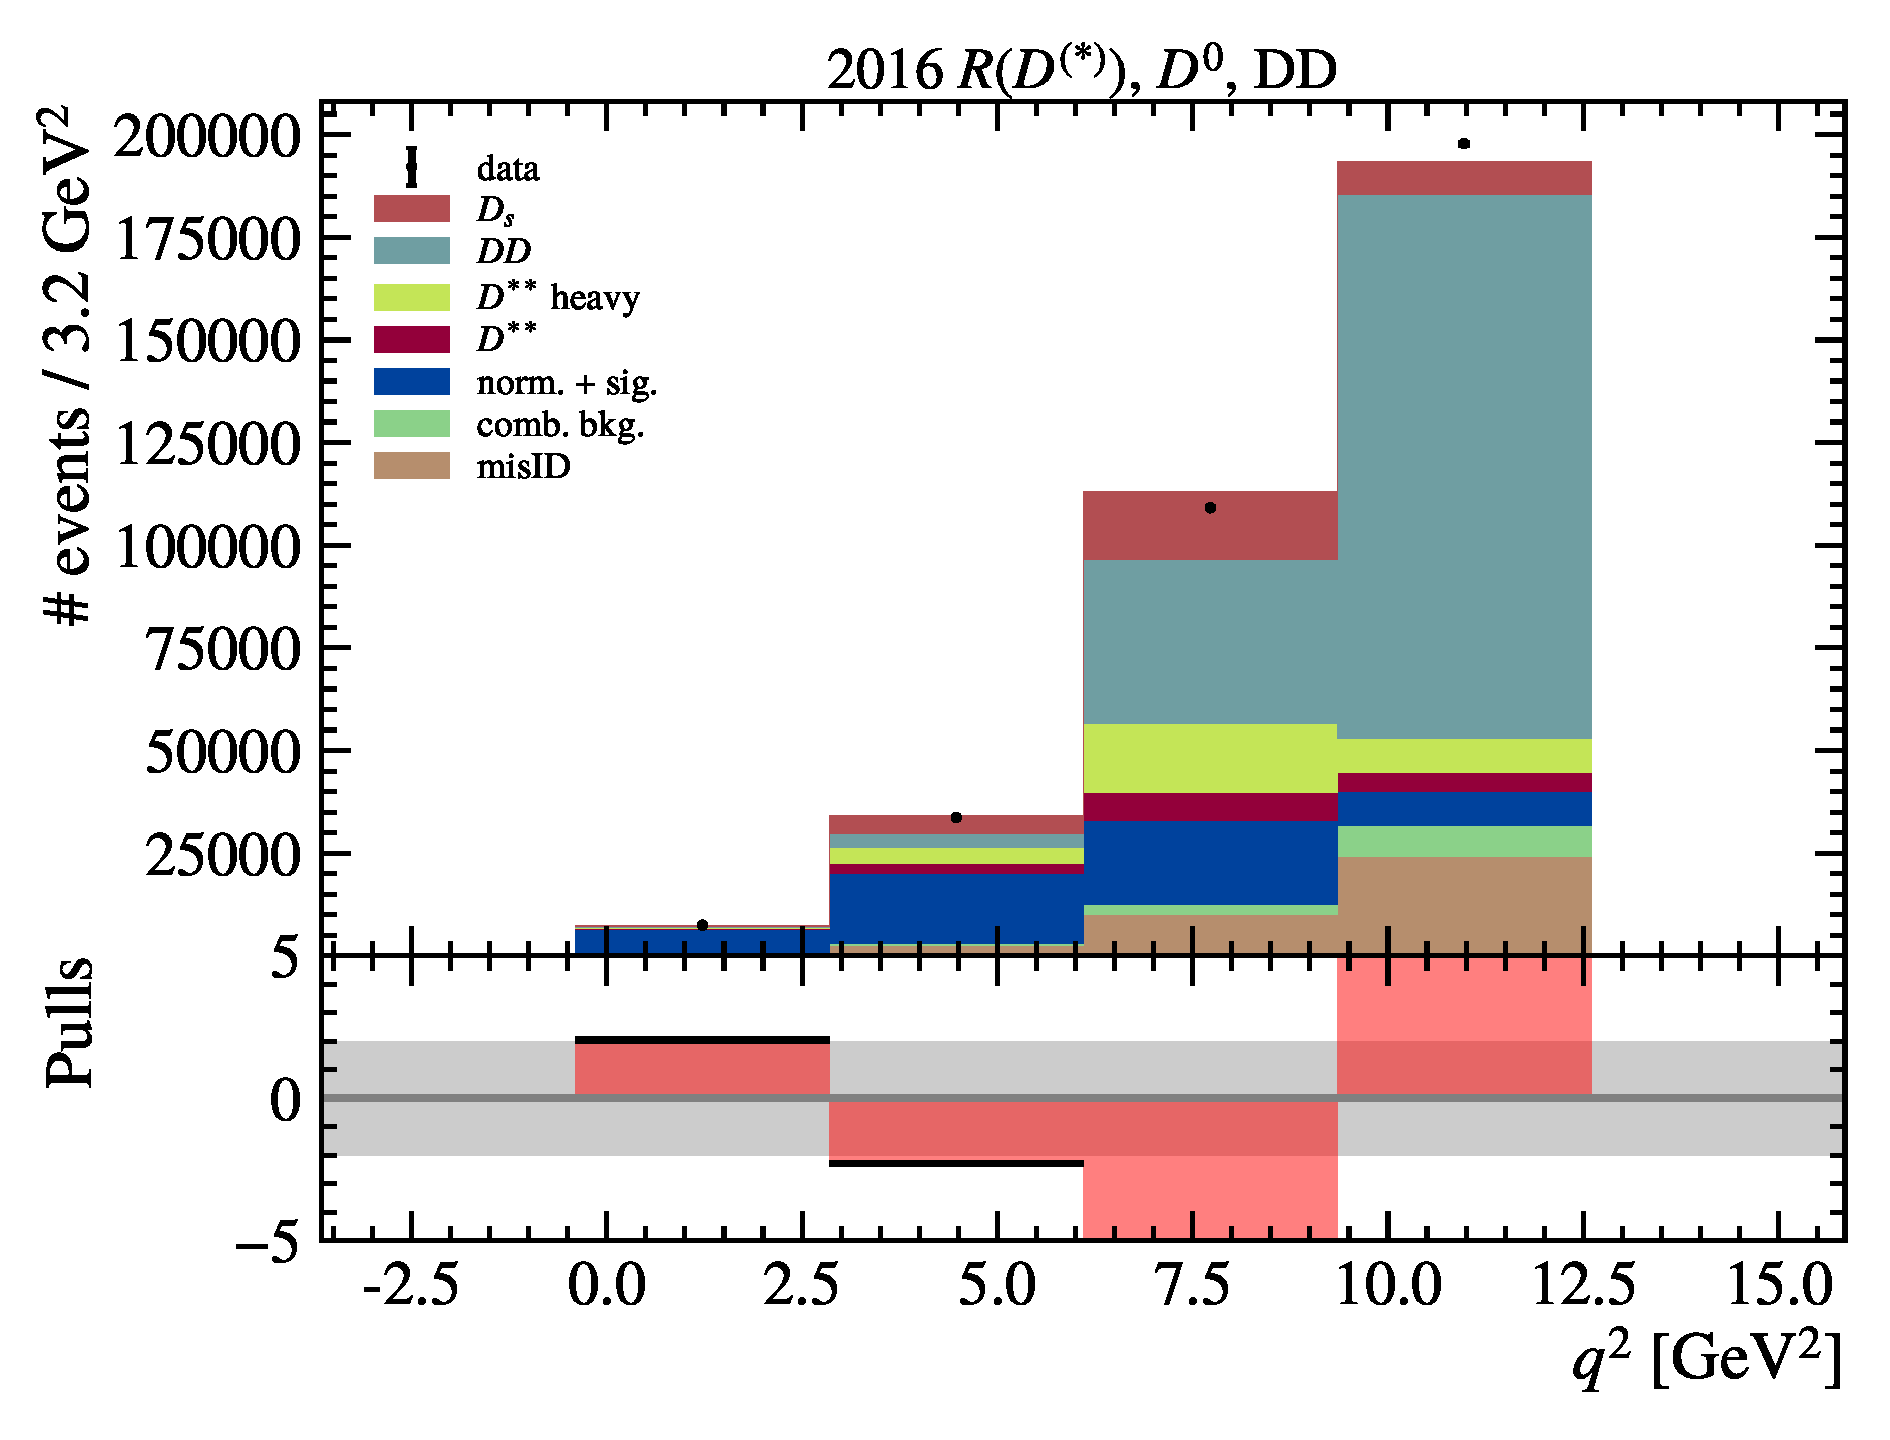
\includegraphics[width=0.32\textwidth]{./figs-supplemental-plots/init-fit/pre-ctrl/fit_result-stacked-D0-dd-q2.pdf}
        \caption{DD}
    \end{subfigure}
    \caption{
        Pre-control fit of \emph{initial fit} in \Dz channel,
        on 1OS, 2OS, and DD samples.
    }
    \label{fig:init-fit-pre-ctrl-d0}
\end{figure}

\begin{figure}[htb]
    \centering
    \begin{subfigure}{\textwidth}
        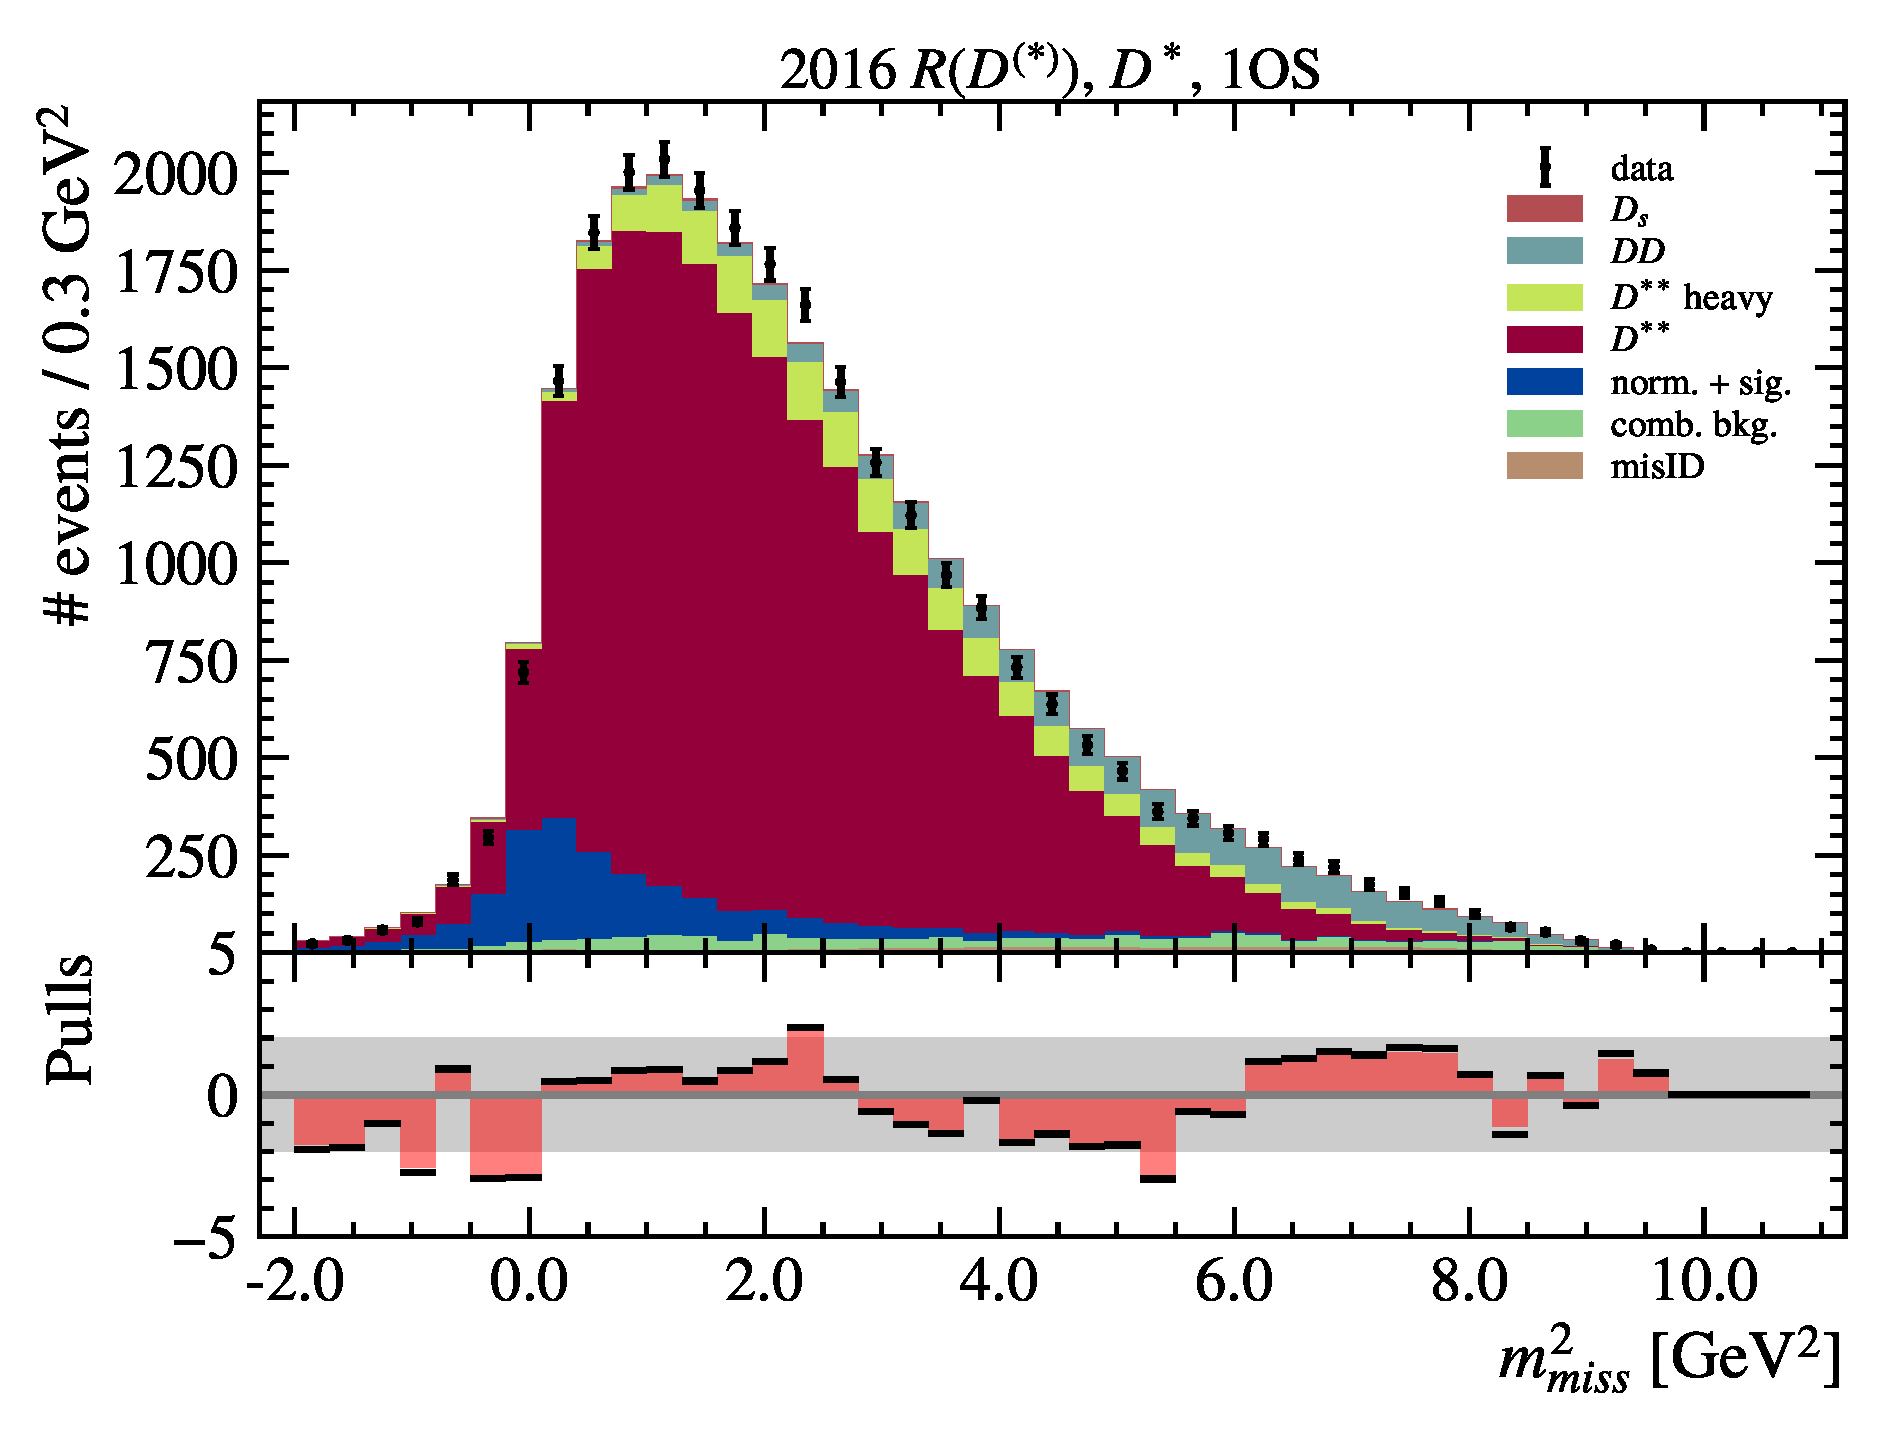
\includegraphics[width=0.32\textwidth]{./figs-supplemental-plots/init-fit/pre-ctrl/fit_result-stacked-Dst-1os-mmiss2.pdf}
        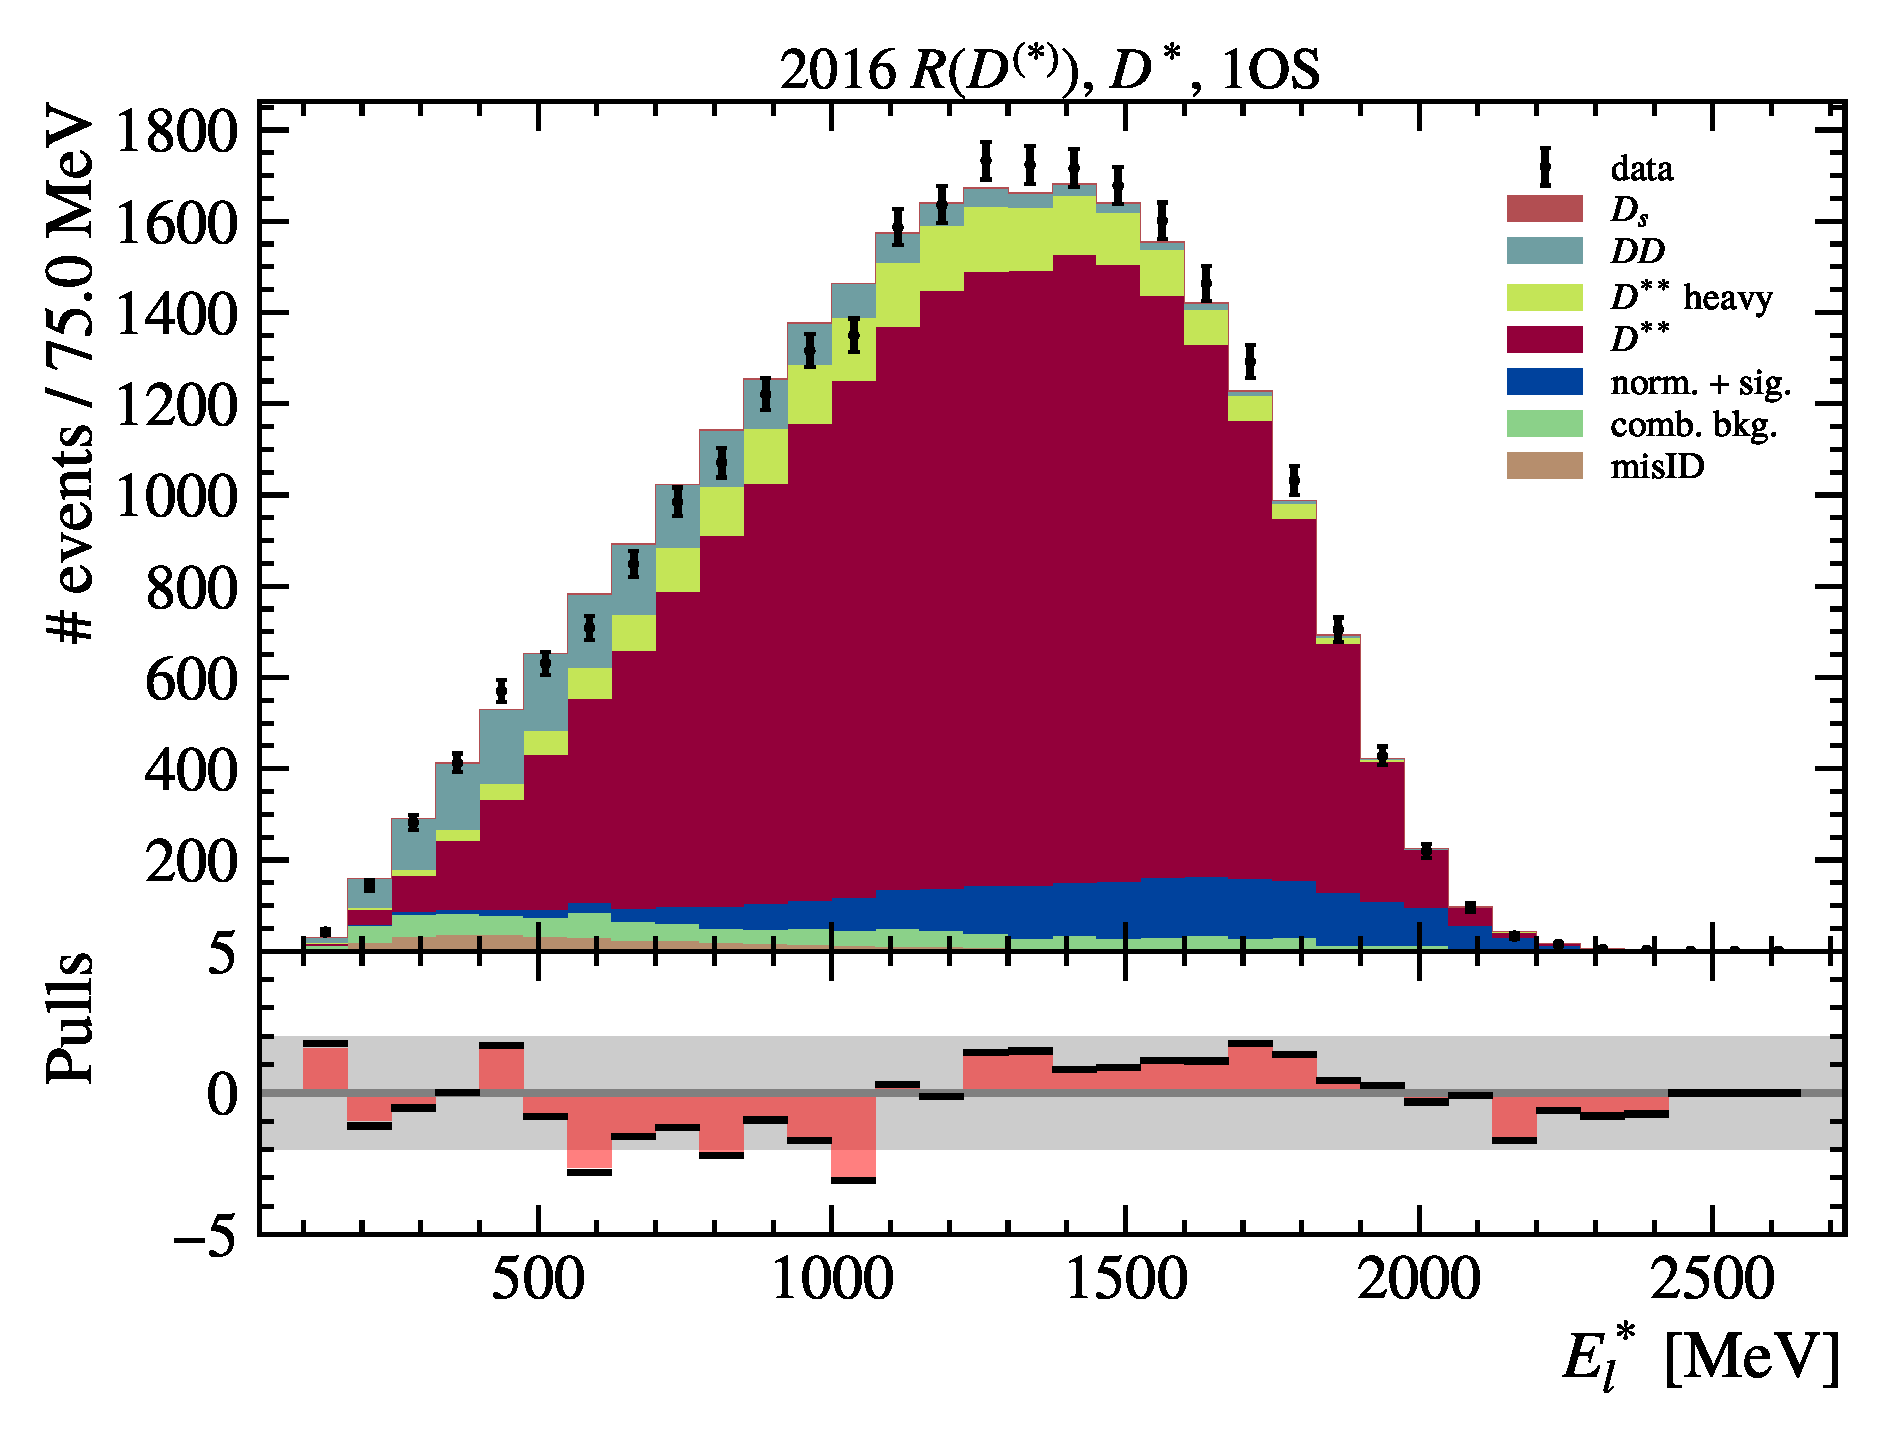
\includegraphics[width=0.32\textwidth]{./figs-supplemental-plots/init-fit/pre-ctrl/fit_result-stacked-Dst-1os-el.pdf}
        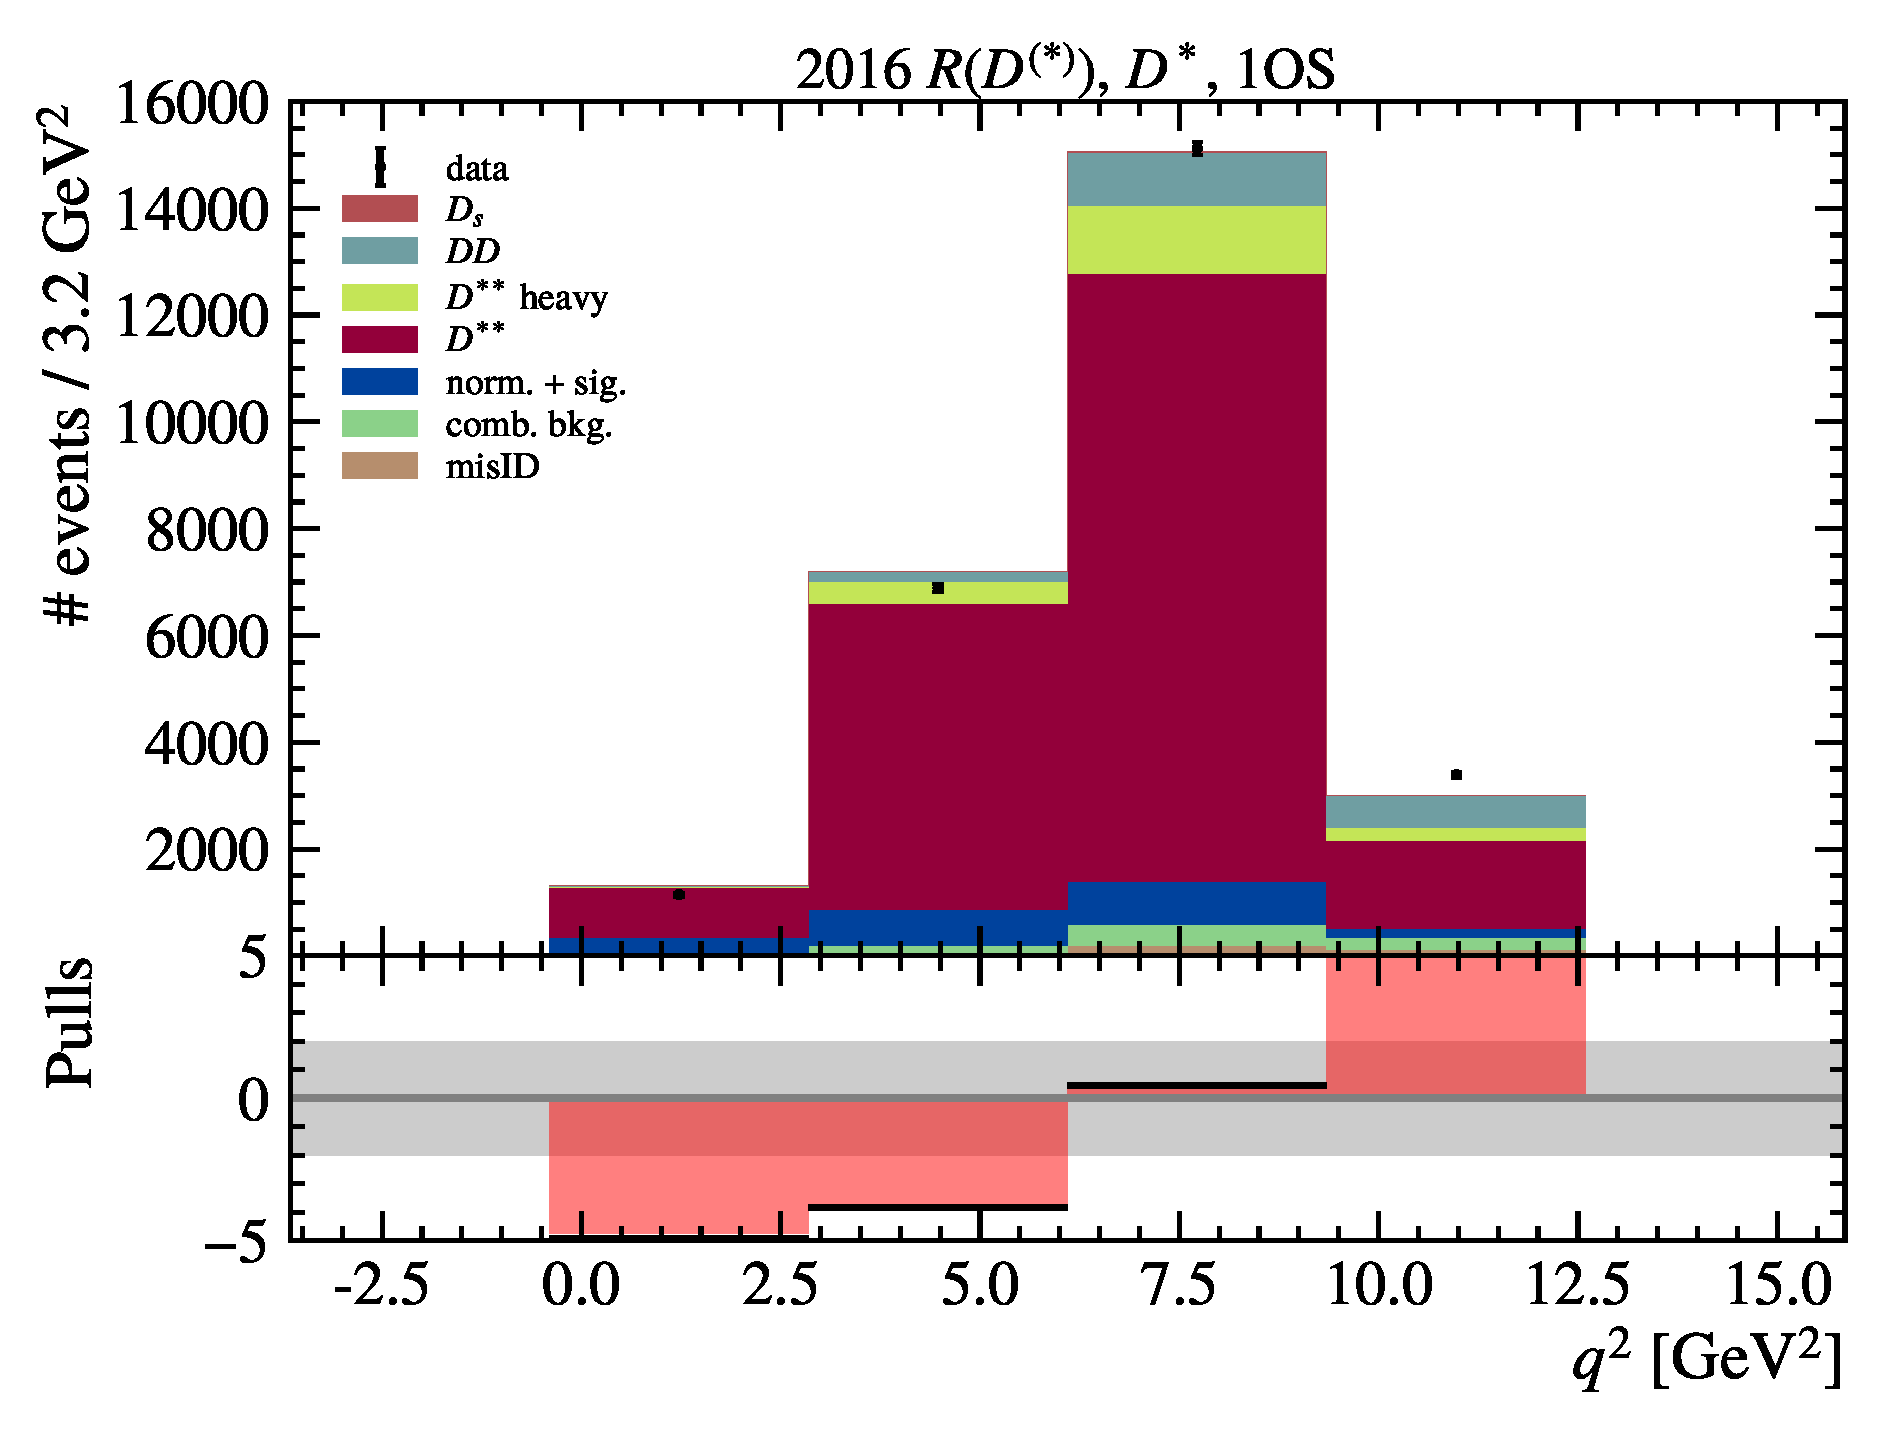
\includegraphics[width=0.32\textwidth]{./figs-supplemental-plots/init-fit/pre-ctrl/fit_result-stacked-Dst-1os-q2.pdf}
        \caption{1OS}
    \end{subfigure}

    \begin{subfigure}{\textwidth}
        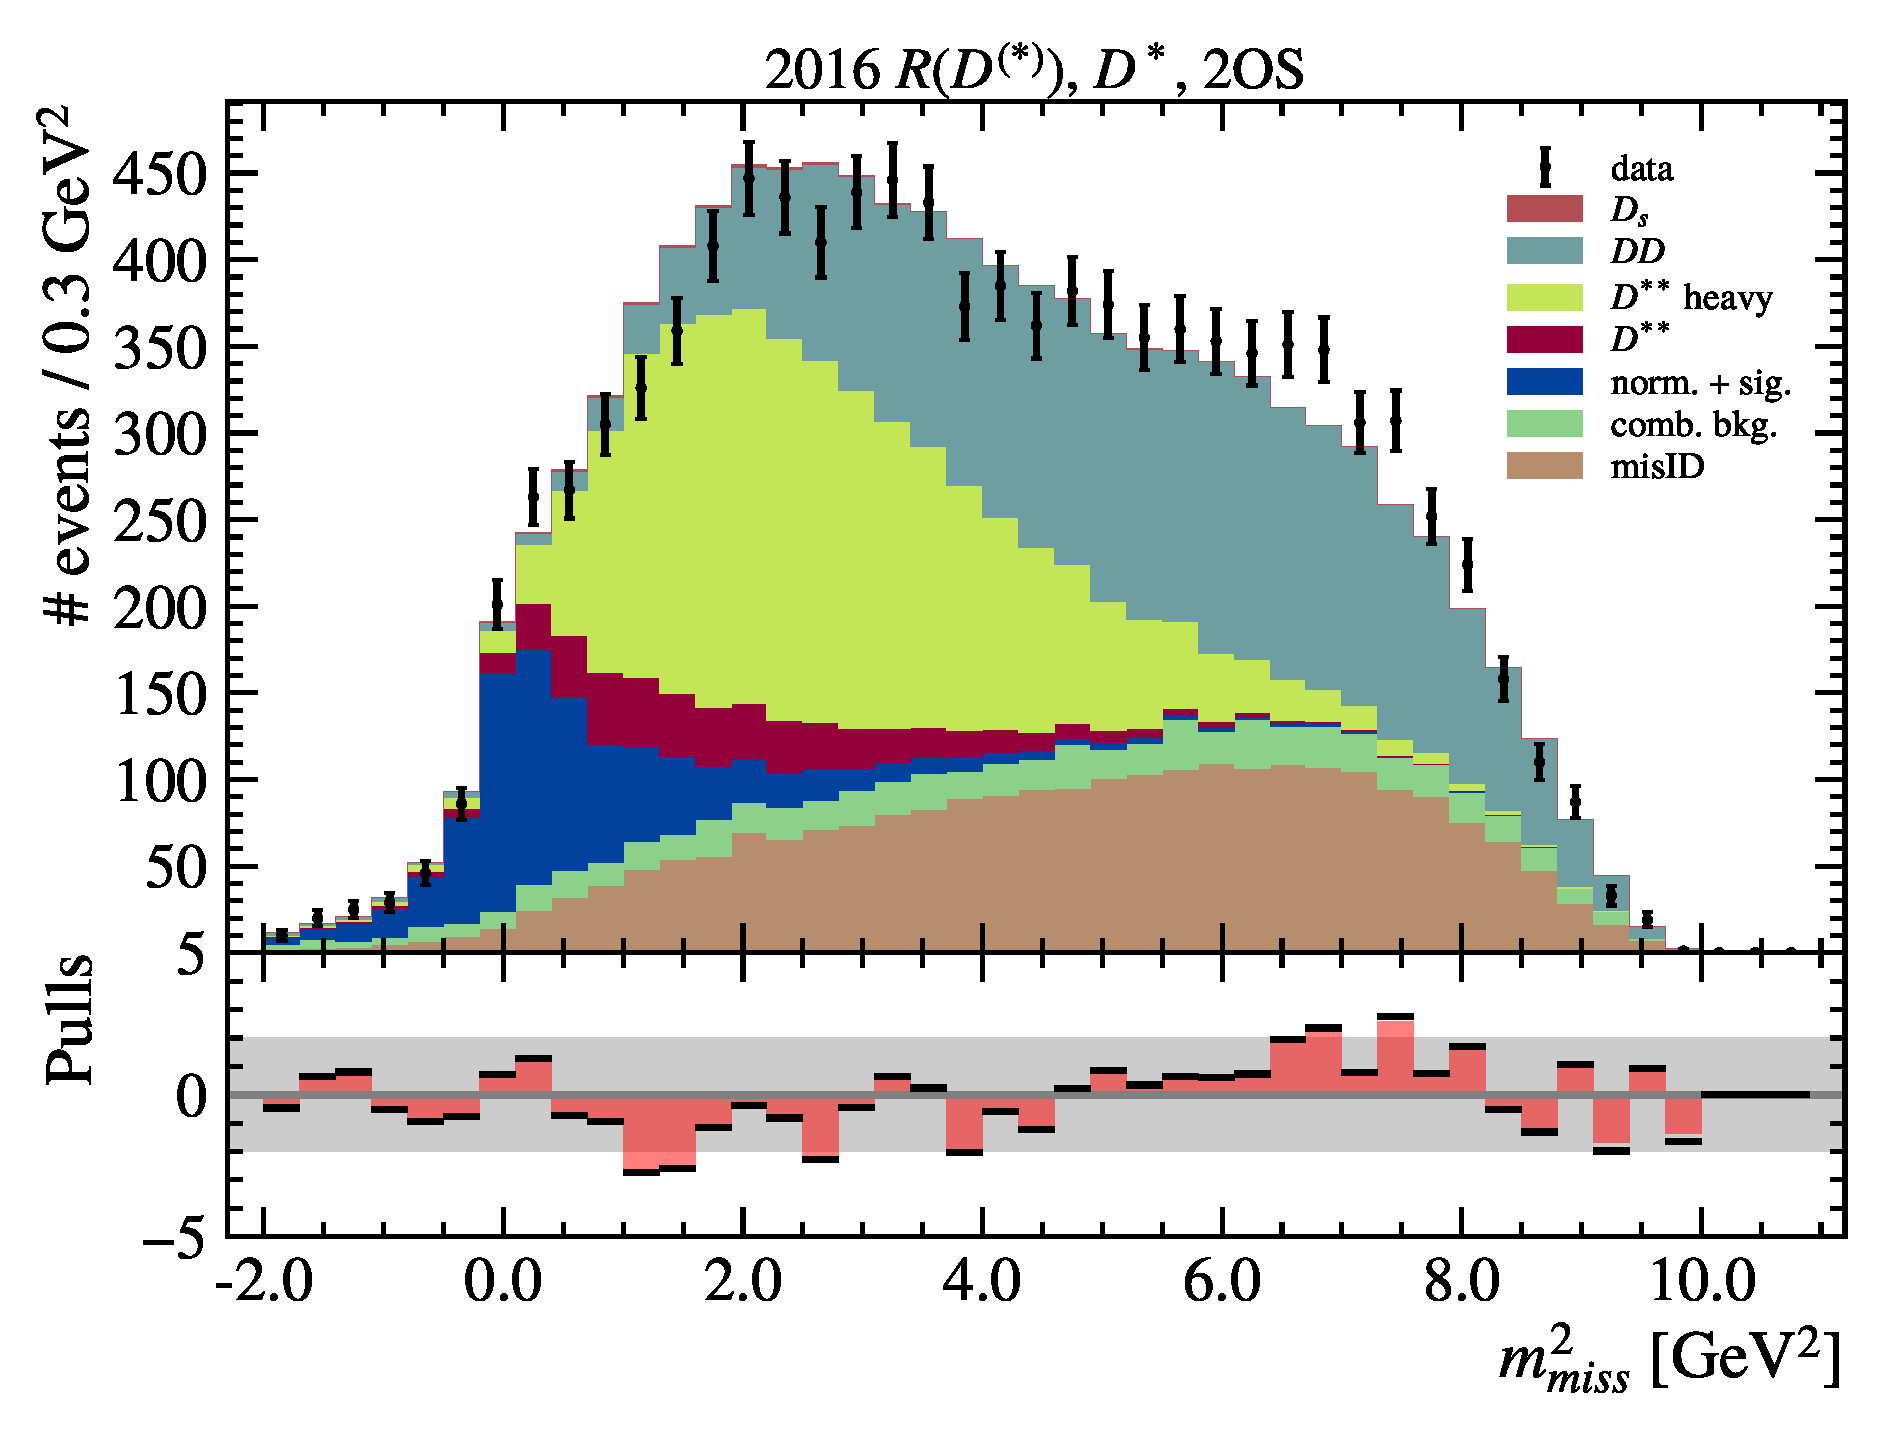
\includegraphics[width=0.32\textwidth]{./figs-supplemental-plots/init-fit/pre-ctrl/fit_result-stacked-Dst-2os-mmiss2.pdf}
        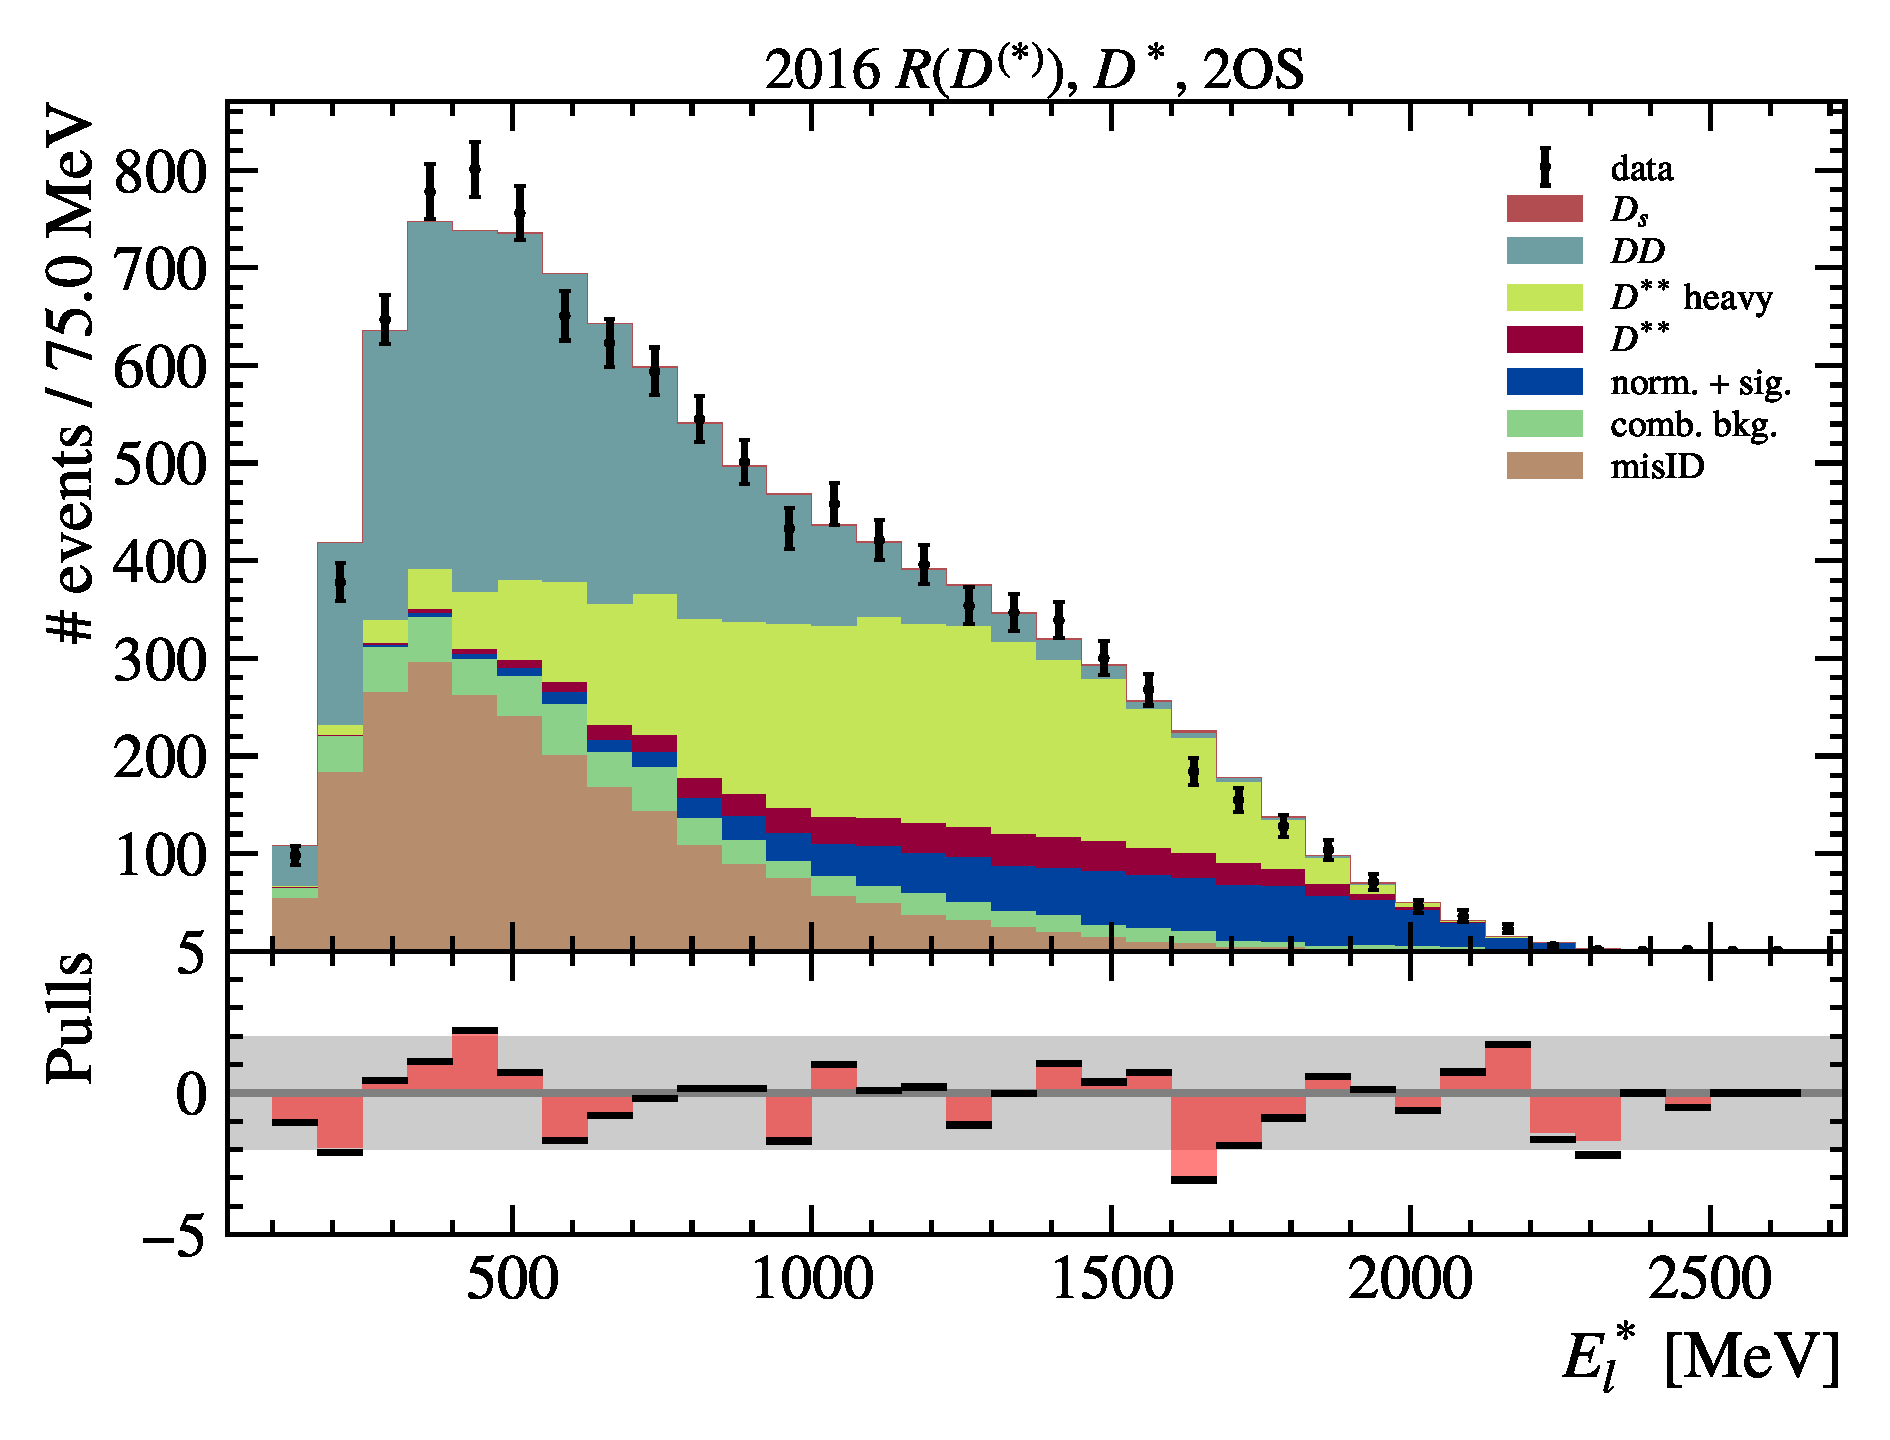
\includegraphics[width=0.32\textwidth]{./figs-supplemental-plots/init-fit/pre-ctrl/fit_result-stacked-Dst-2os-el.pdf}
        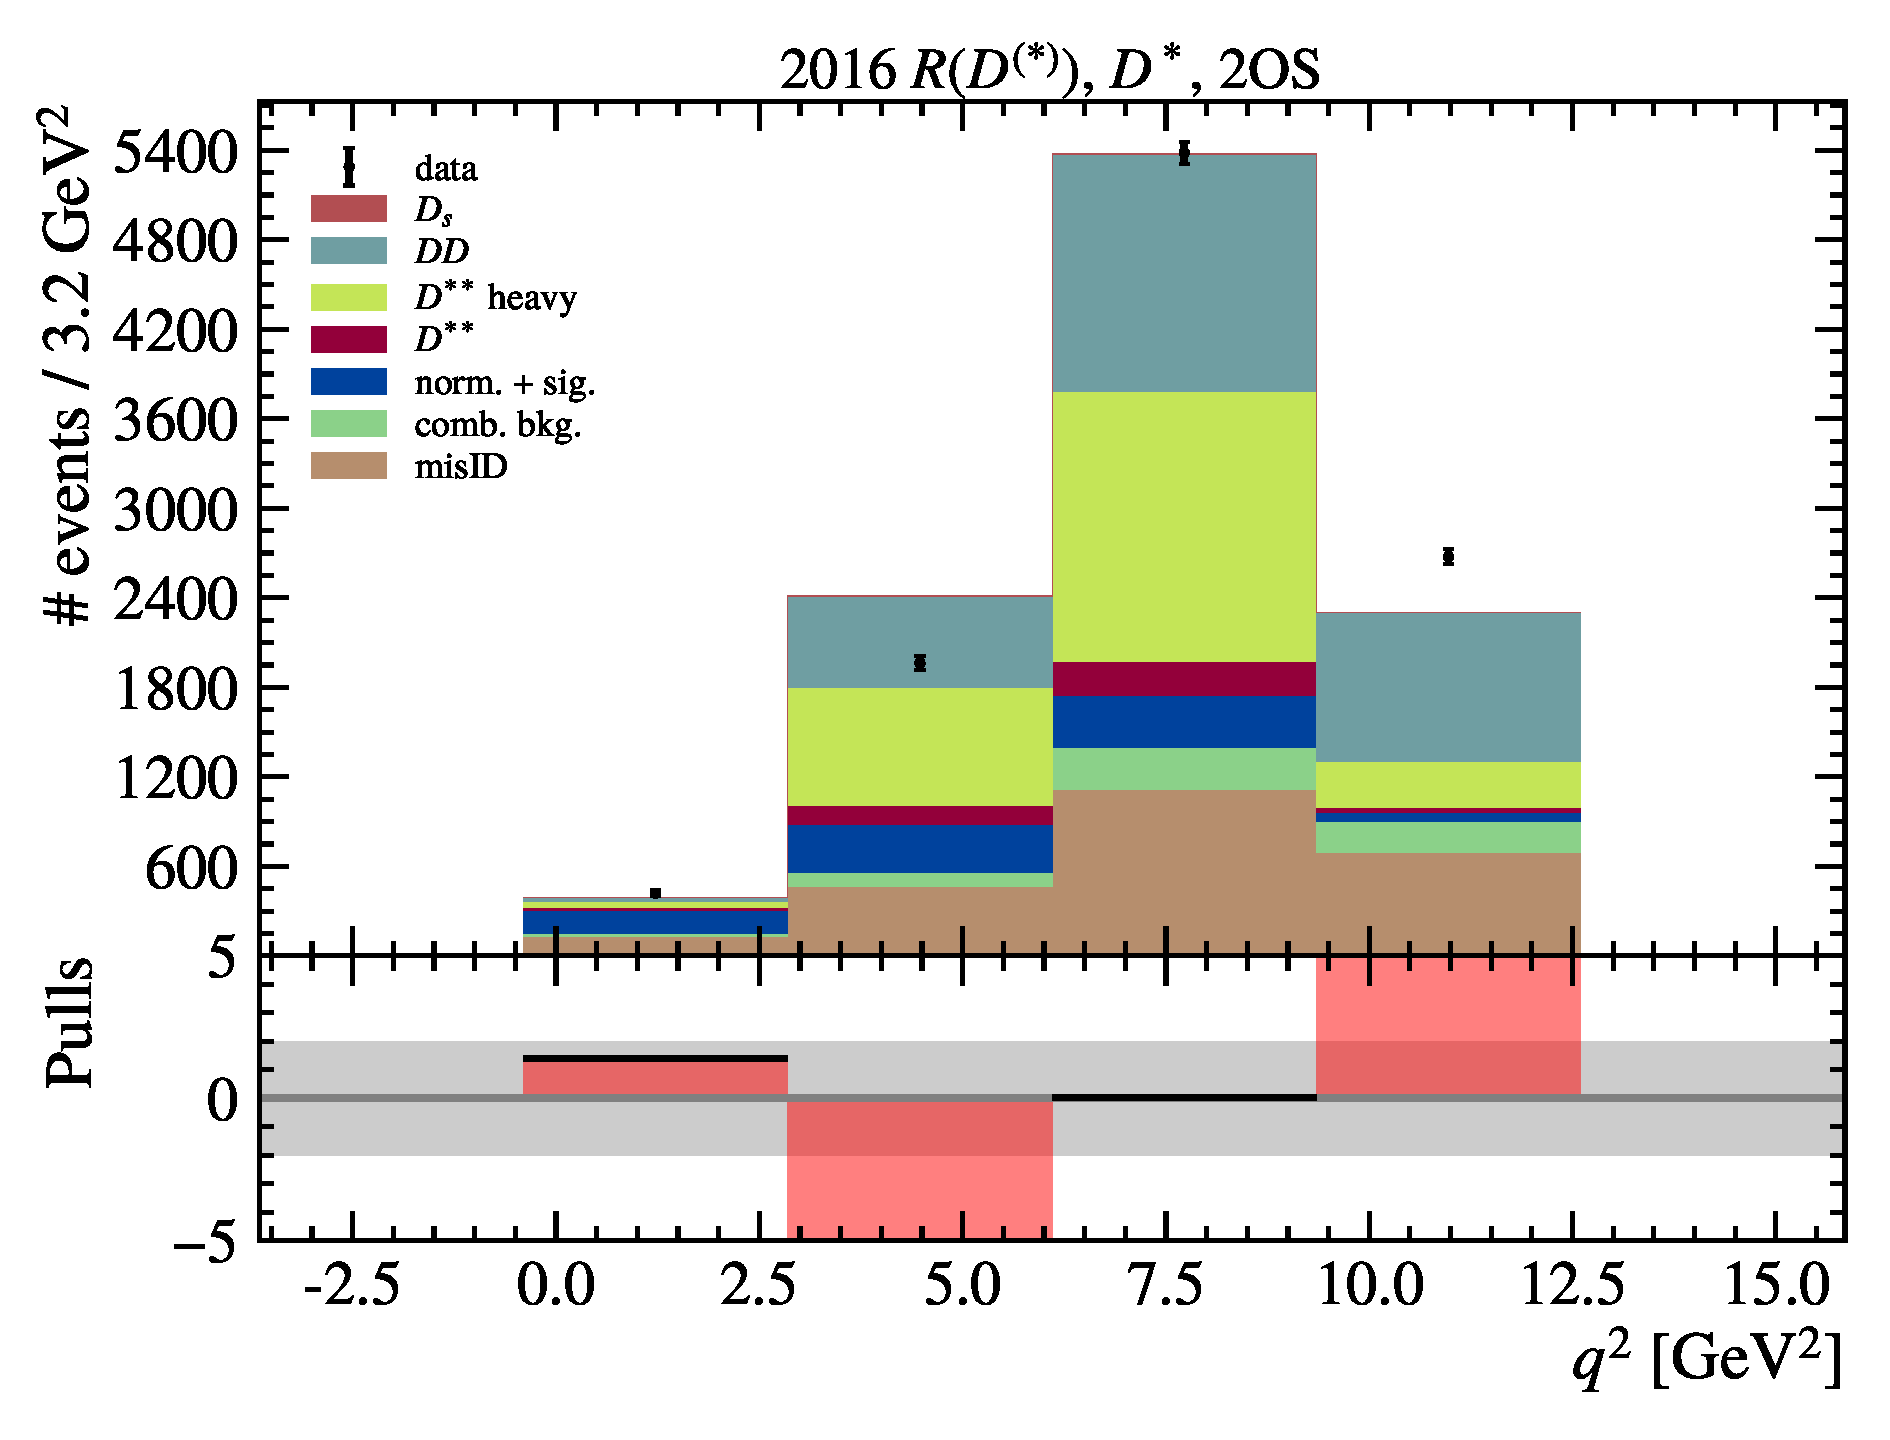
\includegraphics[width=0.32\textwidth]{./figs-supplemental-plots/init-fit/pre-ctrl/fit_result-stacked-Dst-2os-q2.pdf}
        \caption{2OS}
    \end{subfigure}

    \begin{subfigure}{\textwidth}
        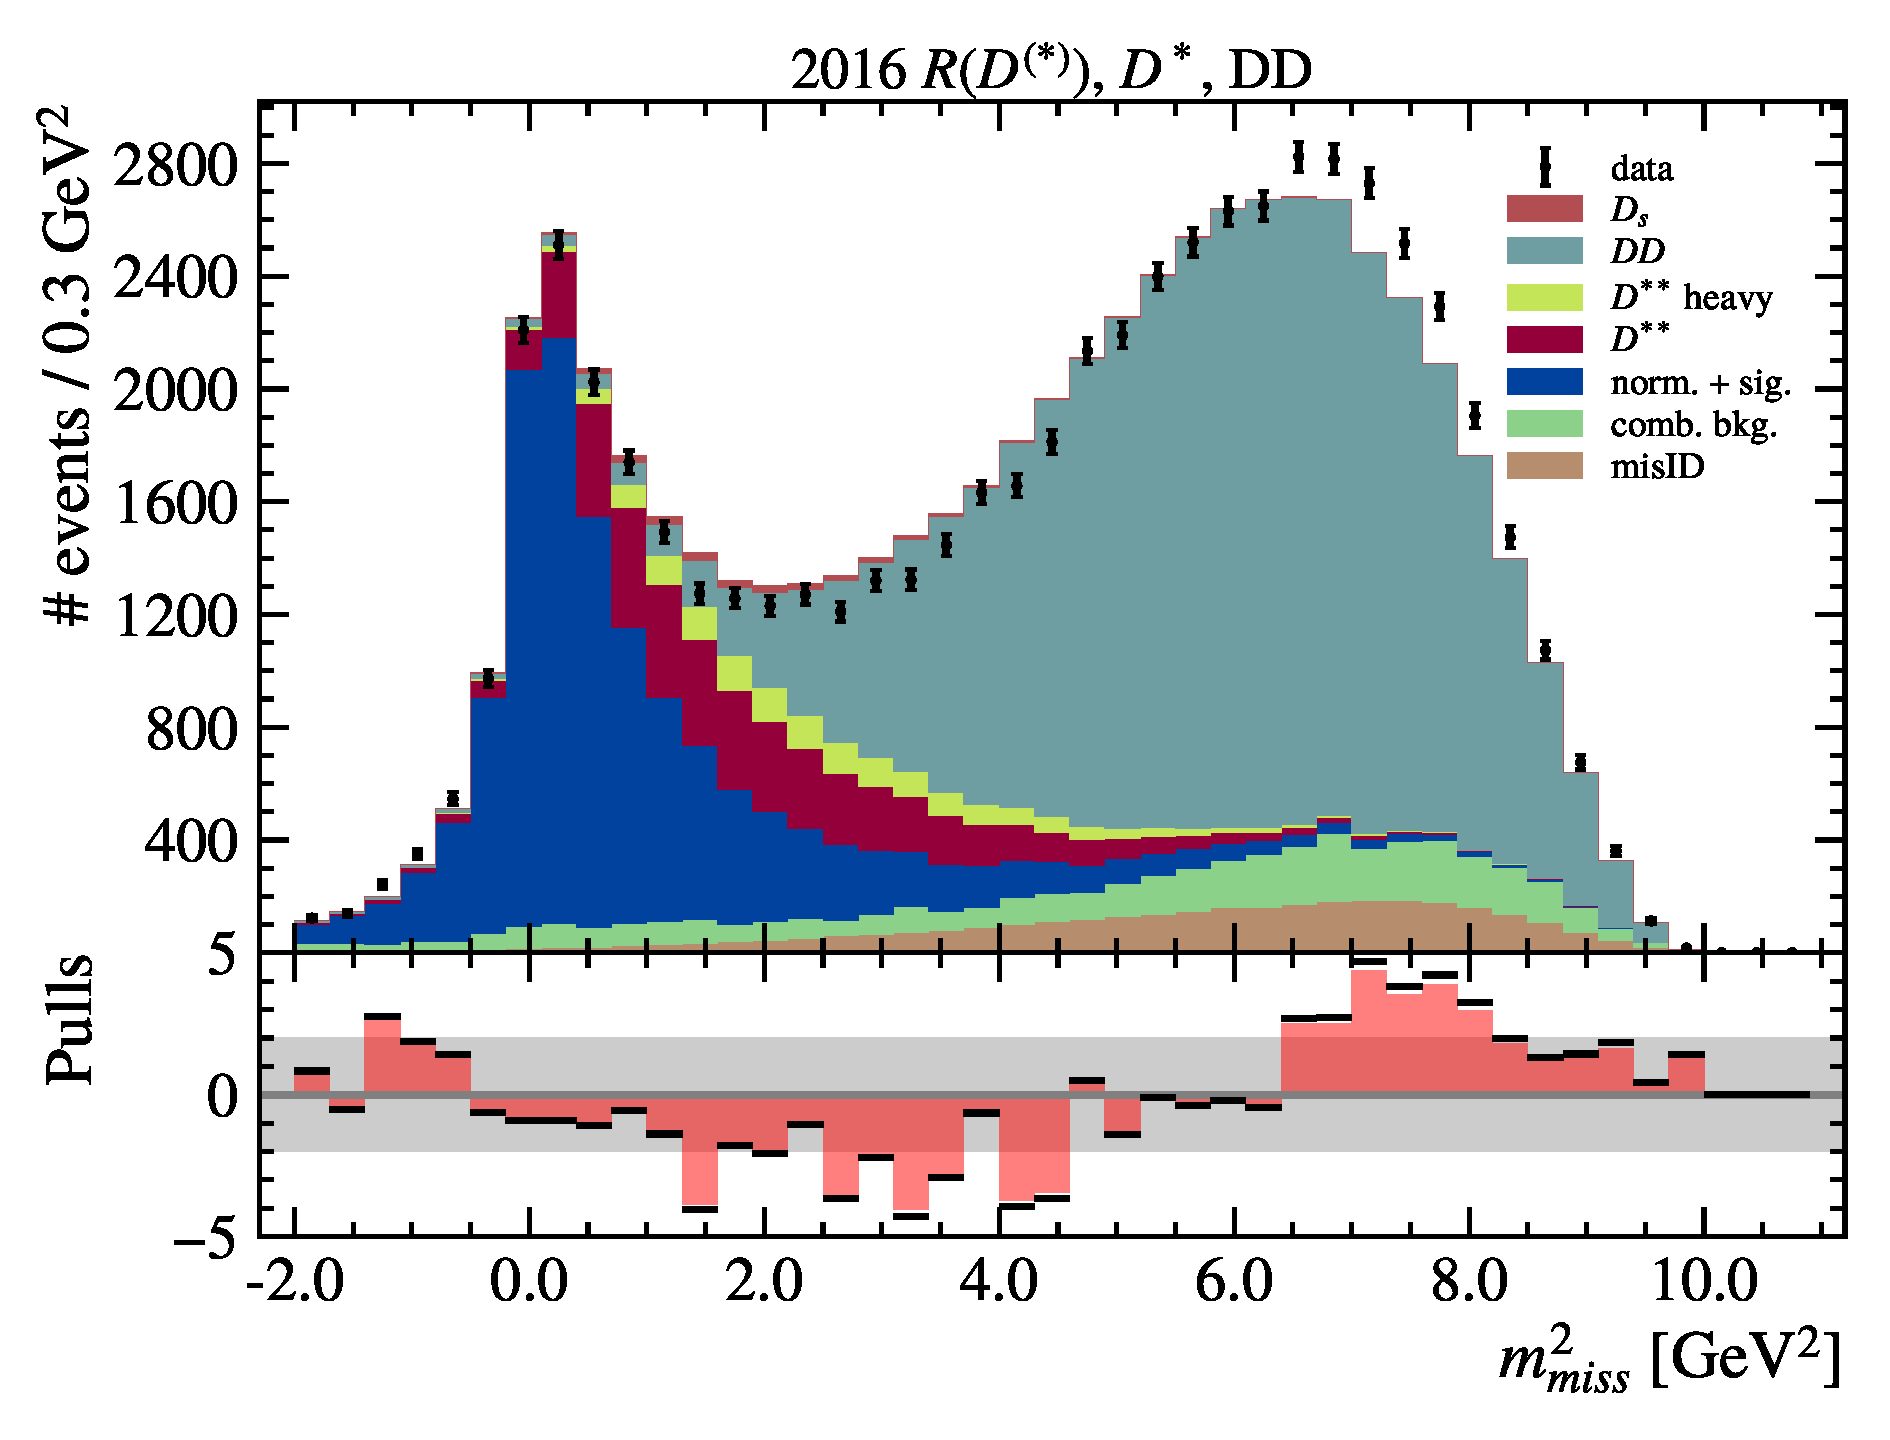
\includegraphics[width=0.32\textwidth]{./figs-supplemental-plots/init-fit/pre-ctrl/fit_result-stacked-Dst-dd-mmiss2.pdf}
        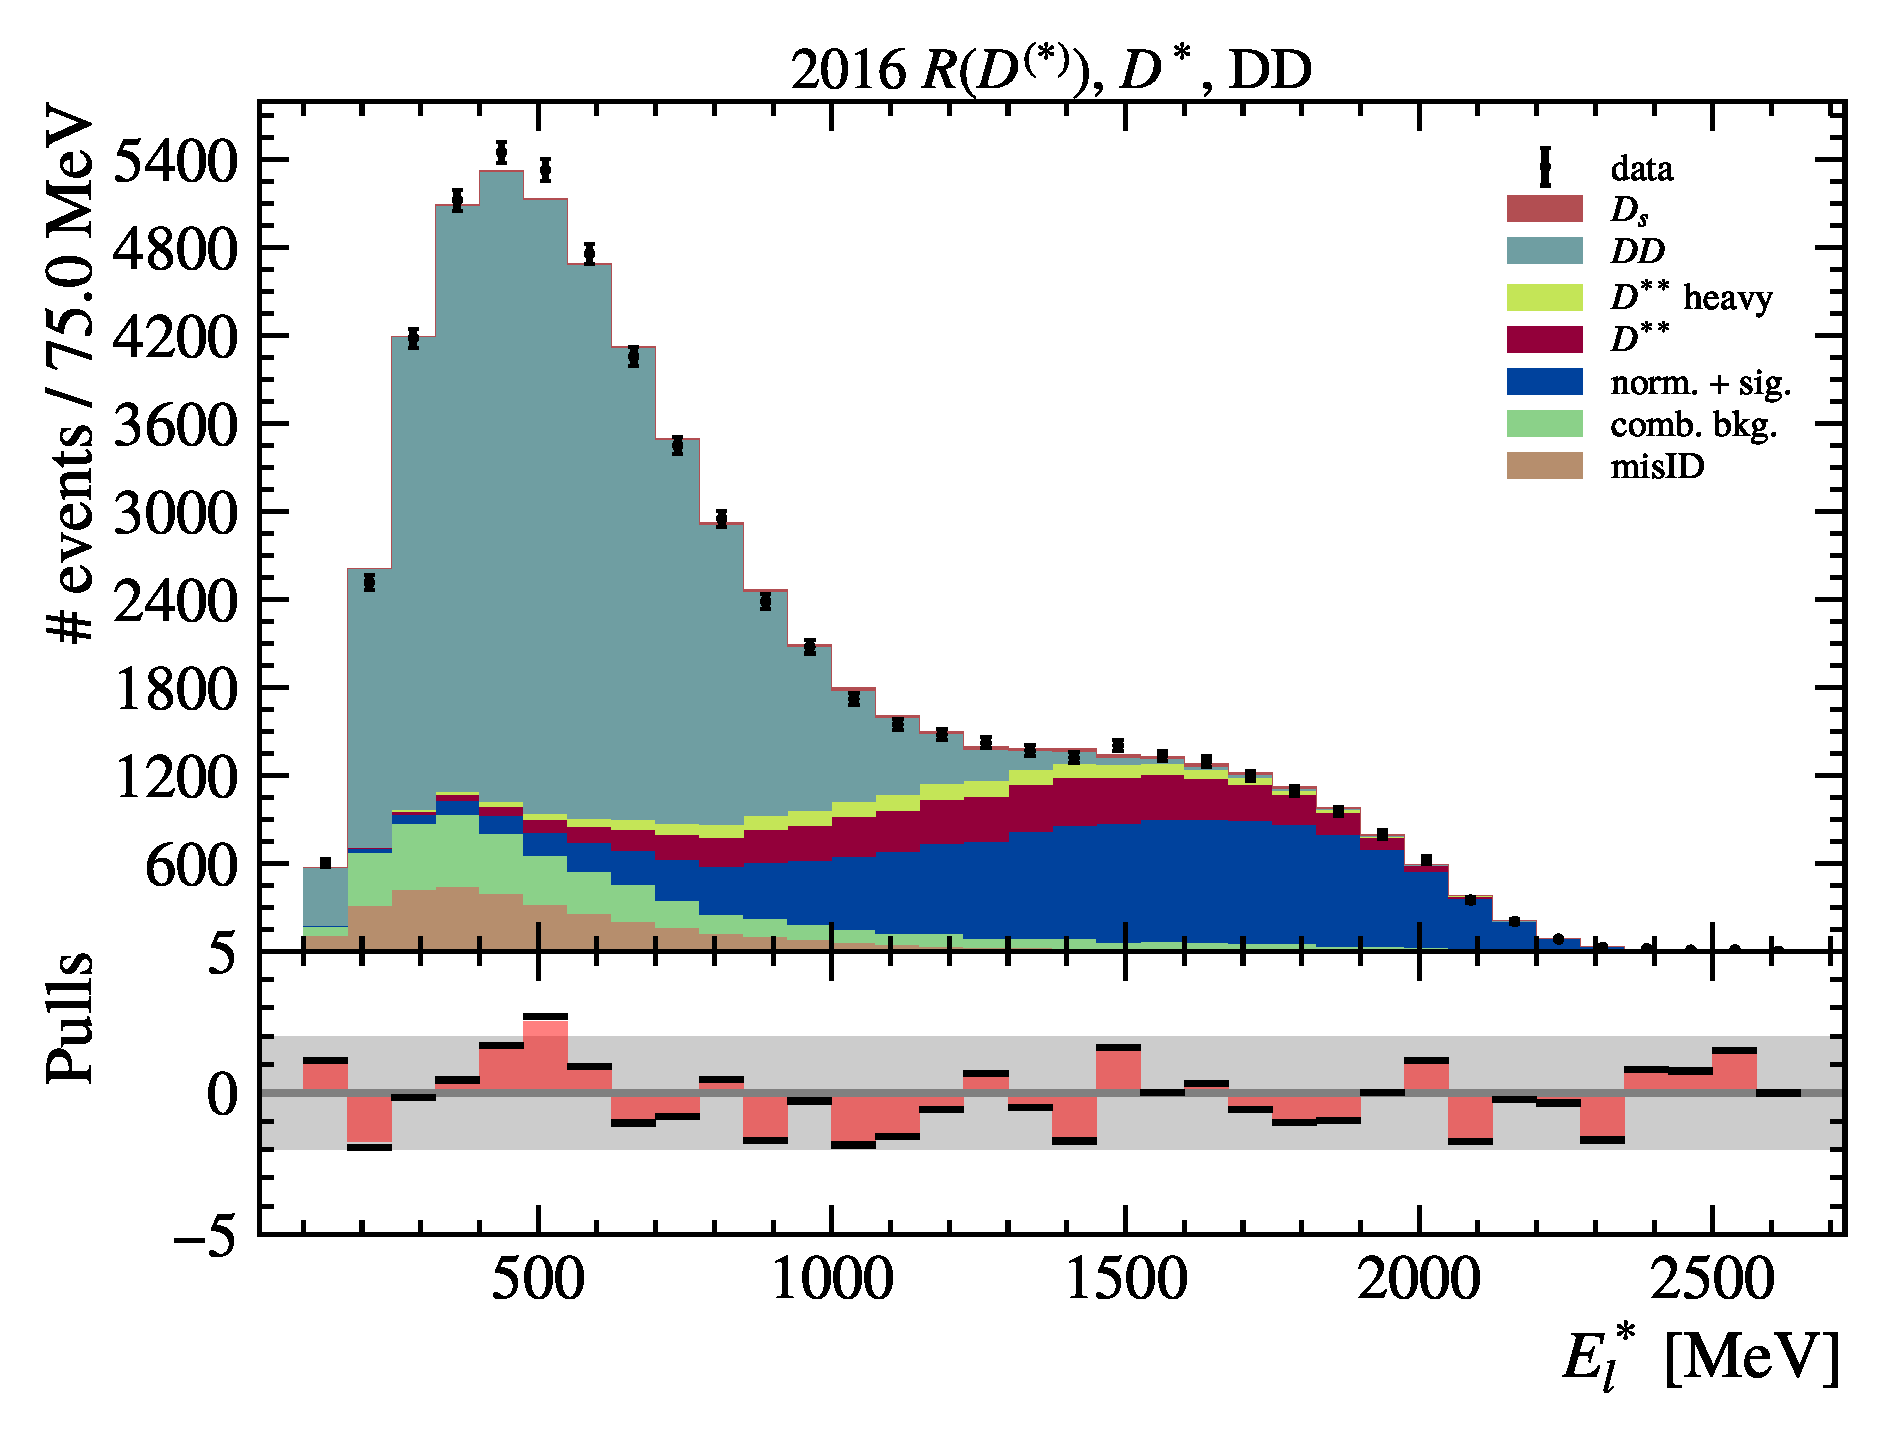
\includegraphics[width=0.32\textwidth]{./figs-supplemental-plots/init-fit/pre-ctrl/fit_result-stacked-Dst-dd-el.pdf}
        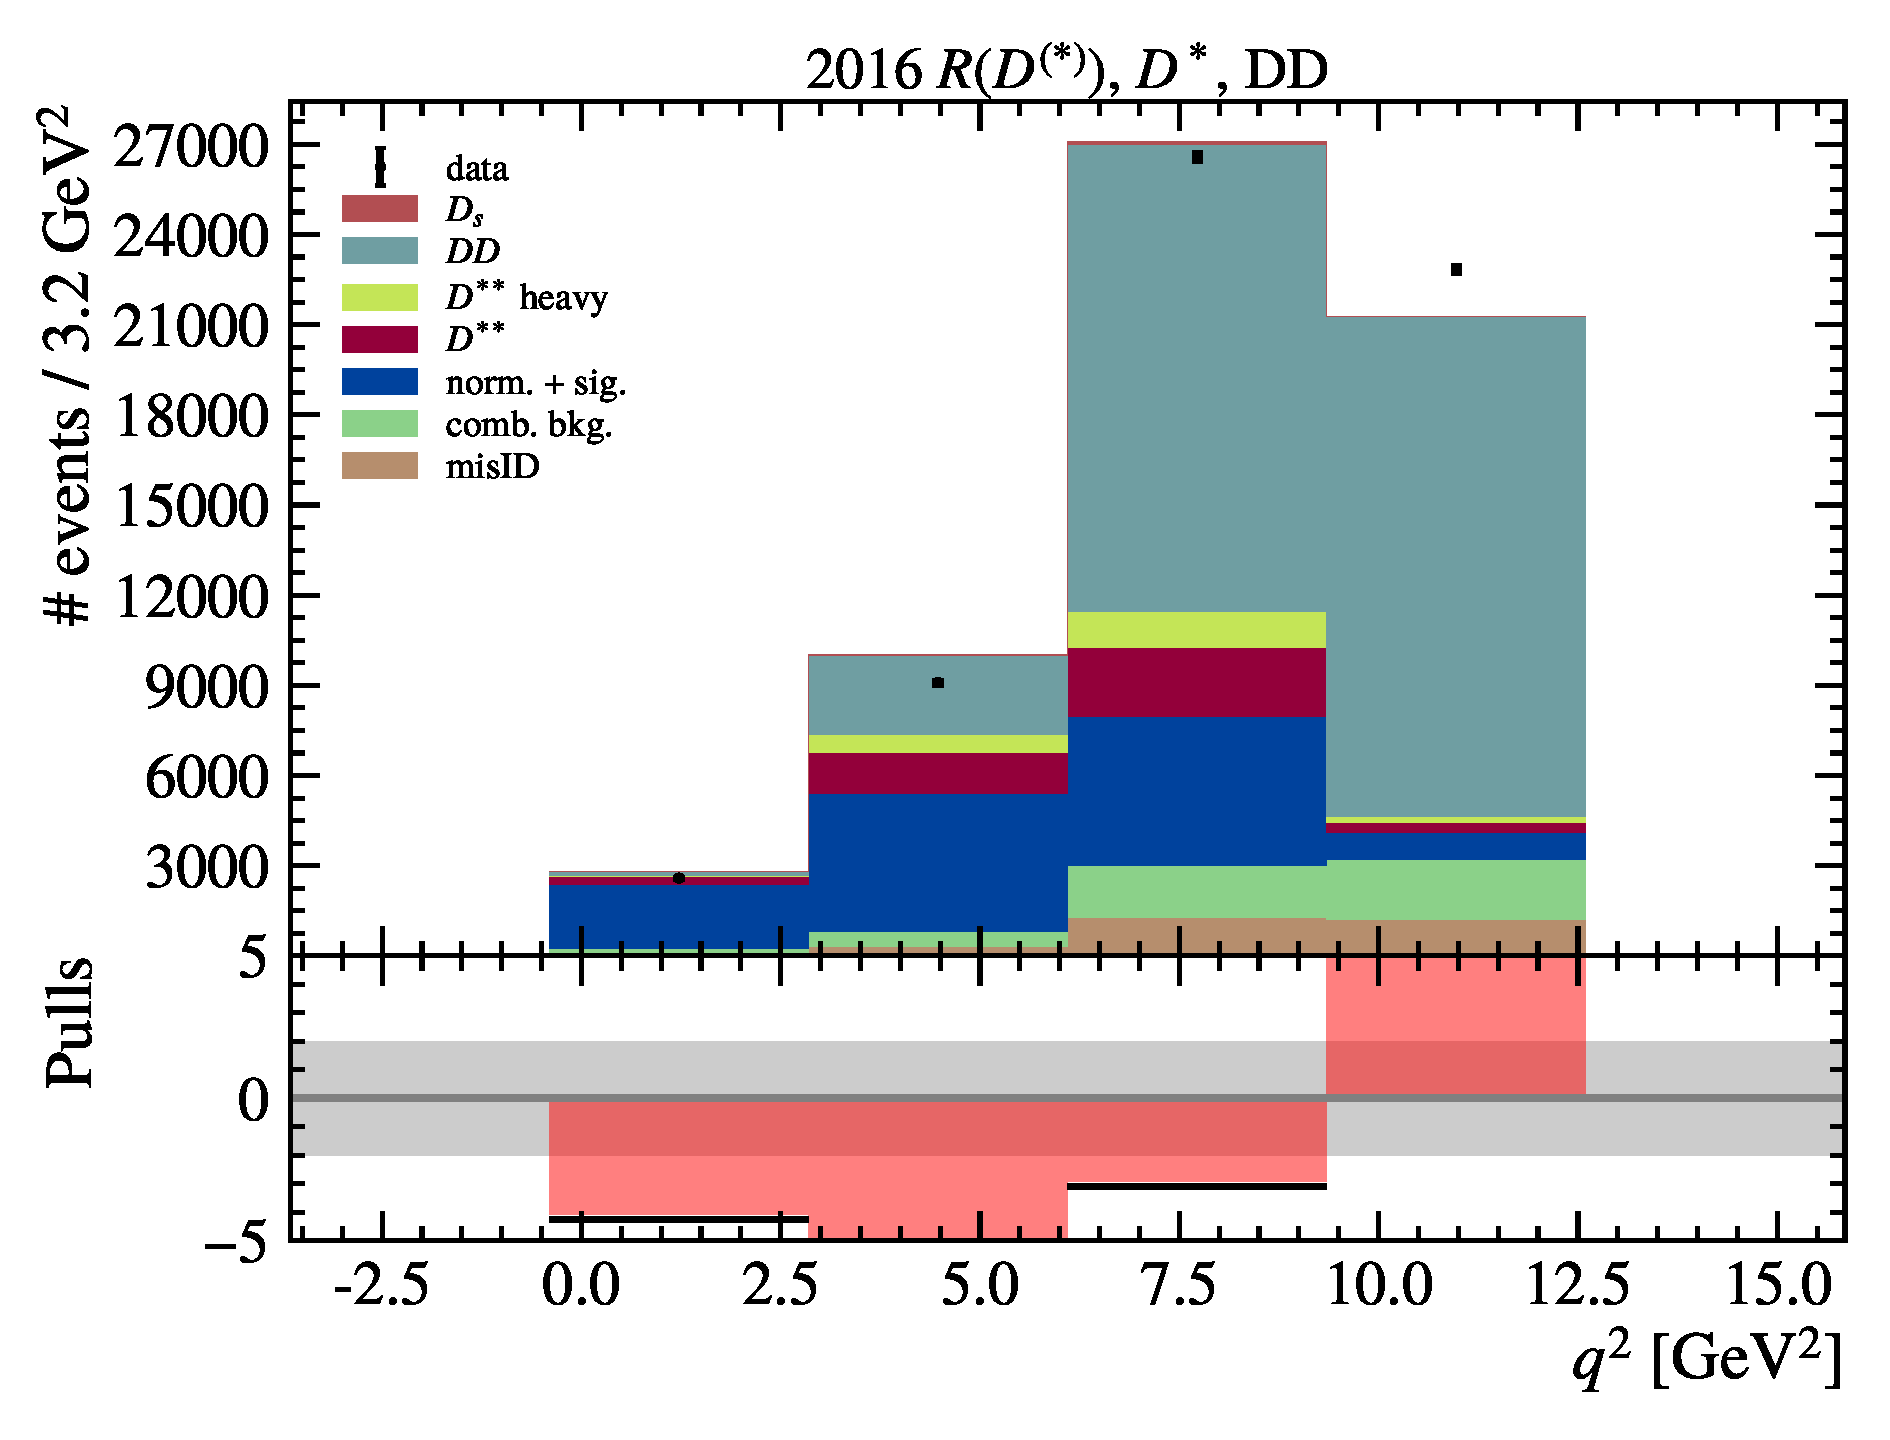
\includegraphics[width=0.32\textwidth]{./figs-supplemental-plots/init-fit/pre-ctrl/fit_result-stacked-Dst-dd-q2.pdf}
        \caption{DD}
    \end{subfigure}
    \caption{
        Pre-control fit of \emph{initial fit} in \Dstar channel,
        on 1OS, 2OS, and DD samples.
    }
    \label{fig:init-fit-pre-ctrl-dst}
\end{figure}

\begin{figure}[htb]
    \centering
    \begin{subfigure}{\textwidth}
        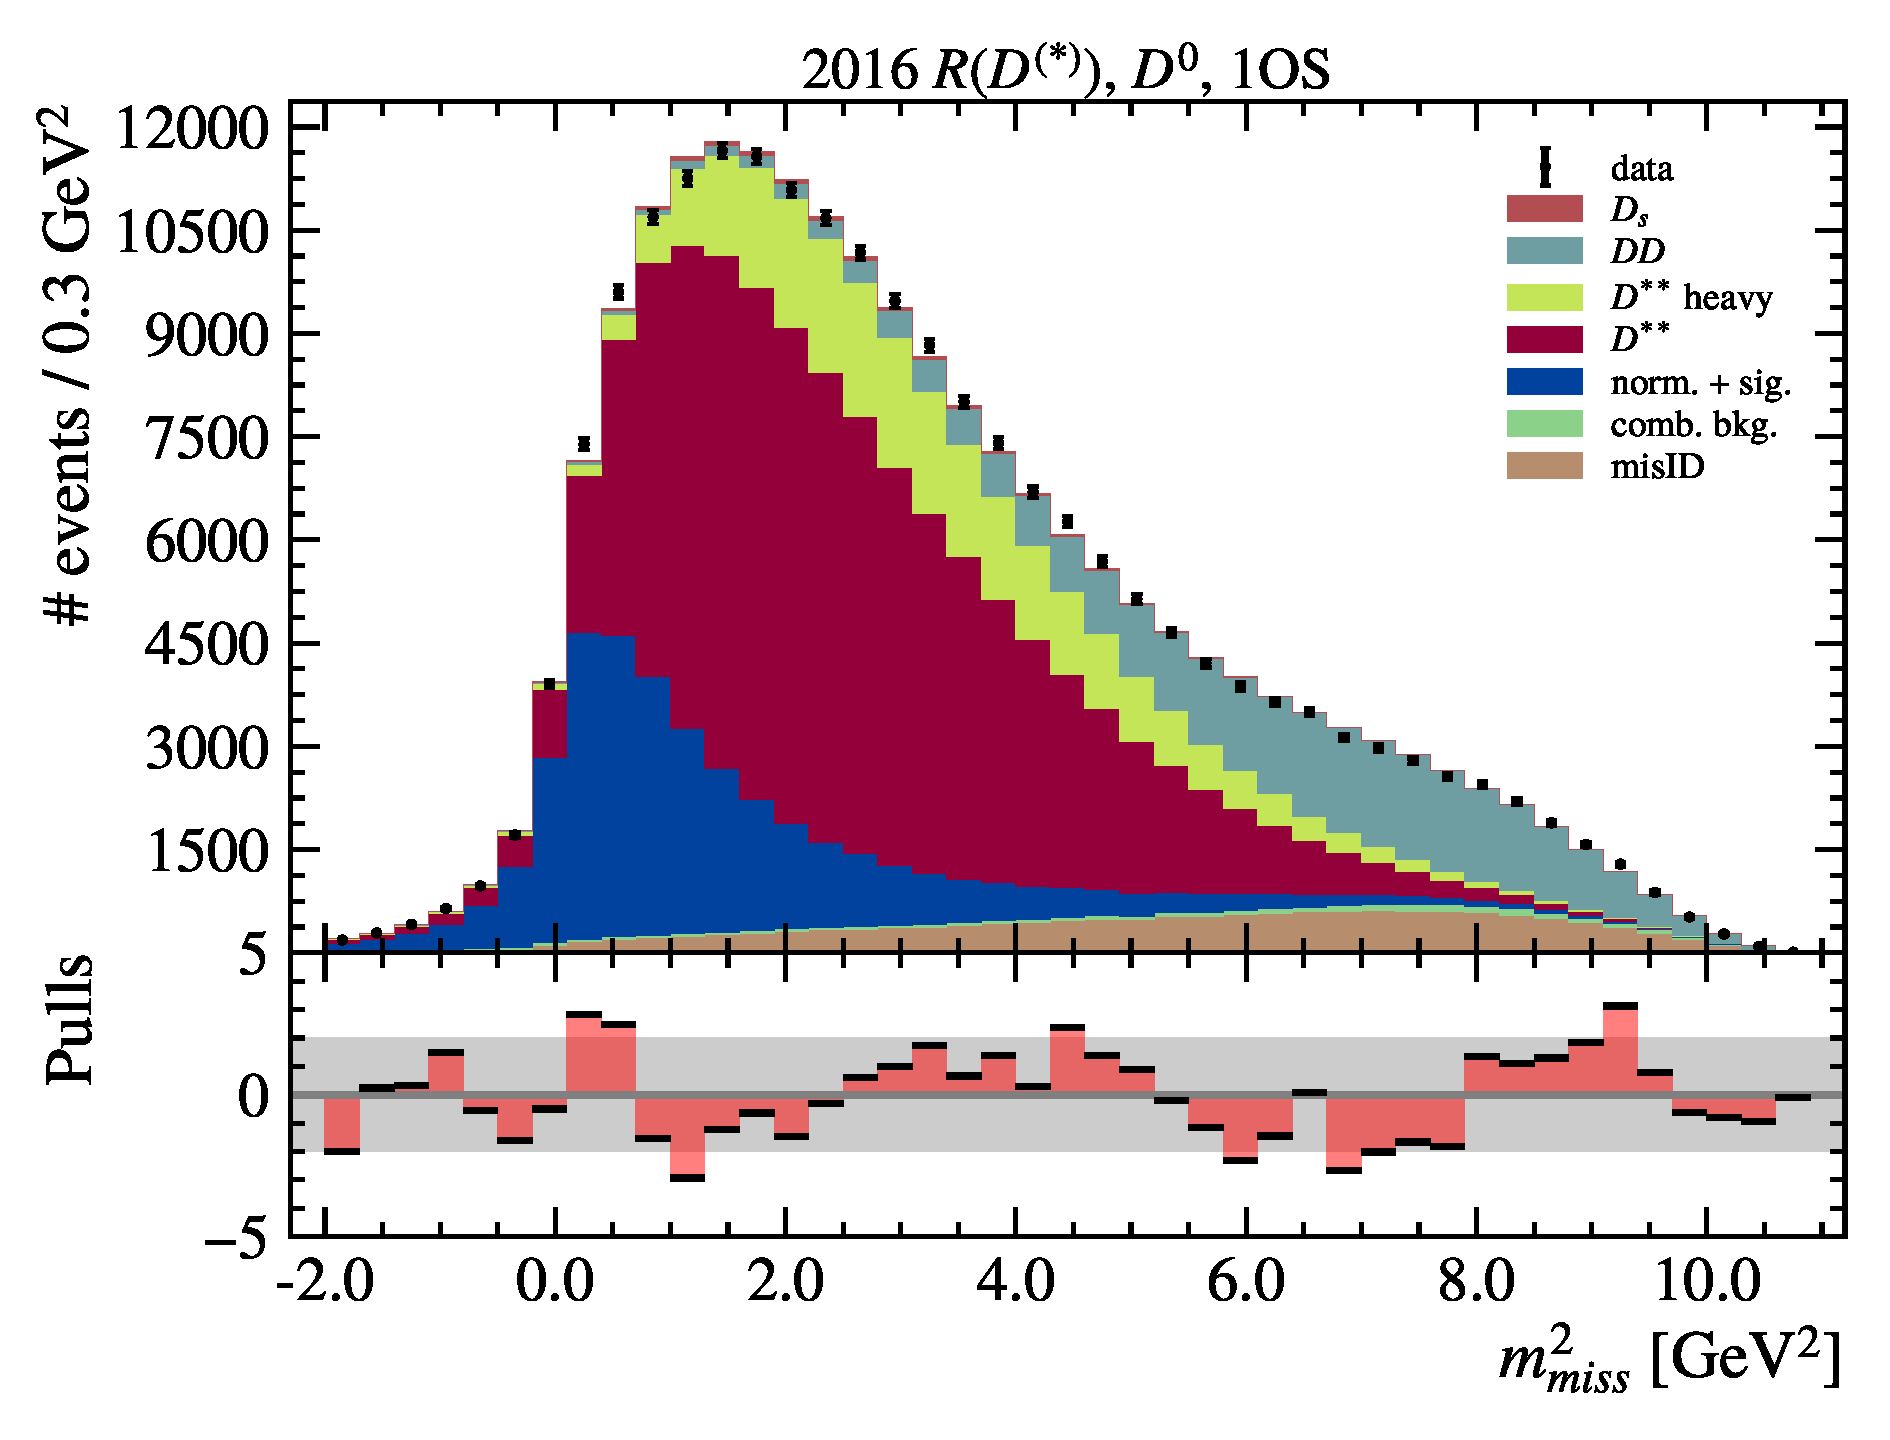
\includegraphics[width=0.32\textwidth]{./figs-supplemental-plots/init-fit/ctrl/fit_result-stacked-D0-1os-mmiss2.pdf}
        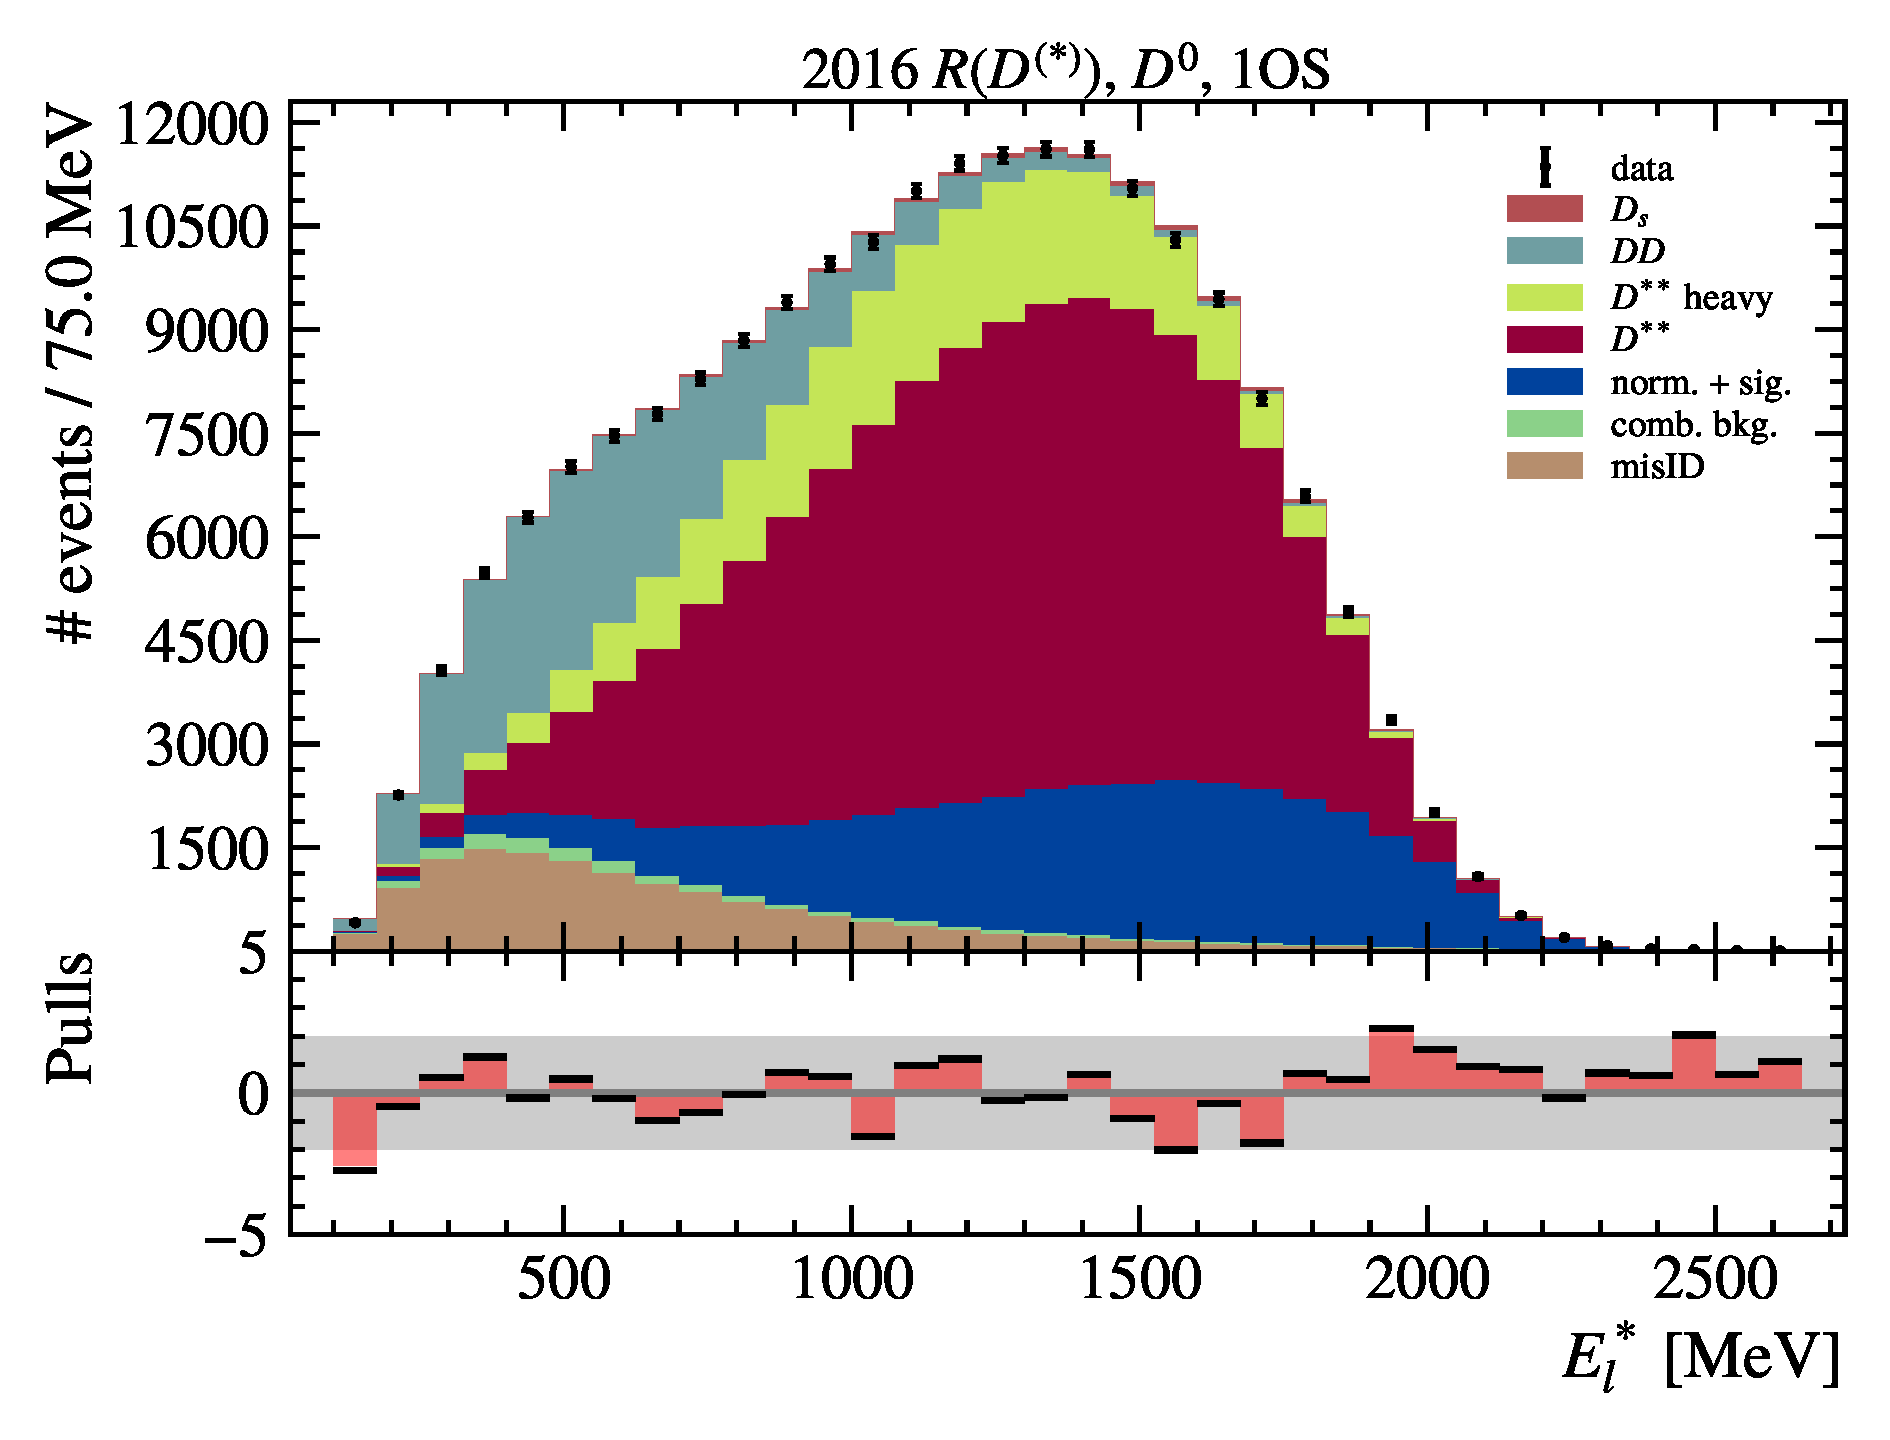
\includegraphics[width=0.32\textwidth]{./figs-supplemental-plots/init-fit/ctrl/fit_result-stacked-D0-1os-el.pdf}
        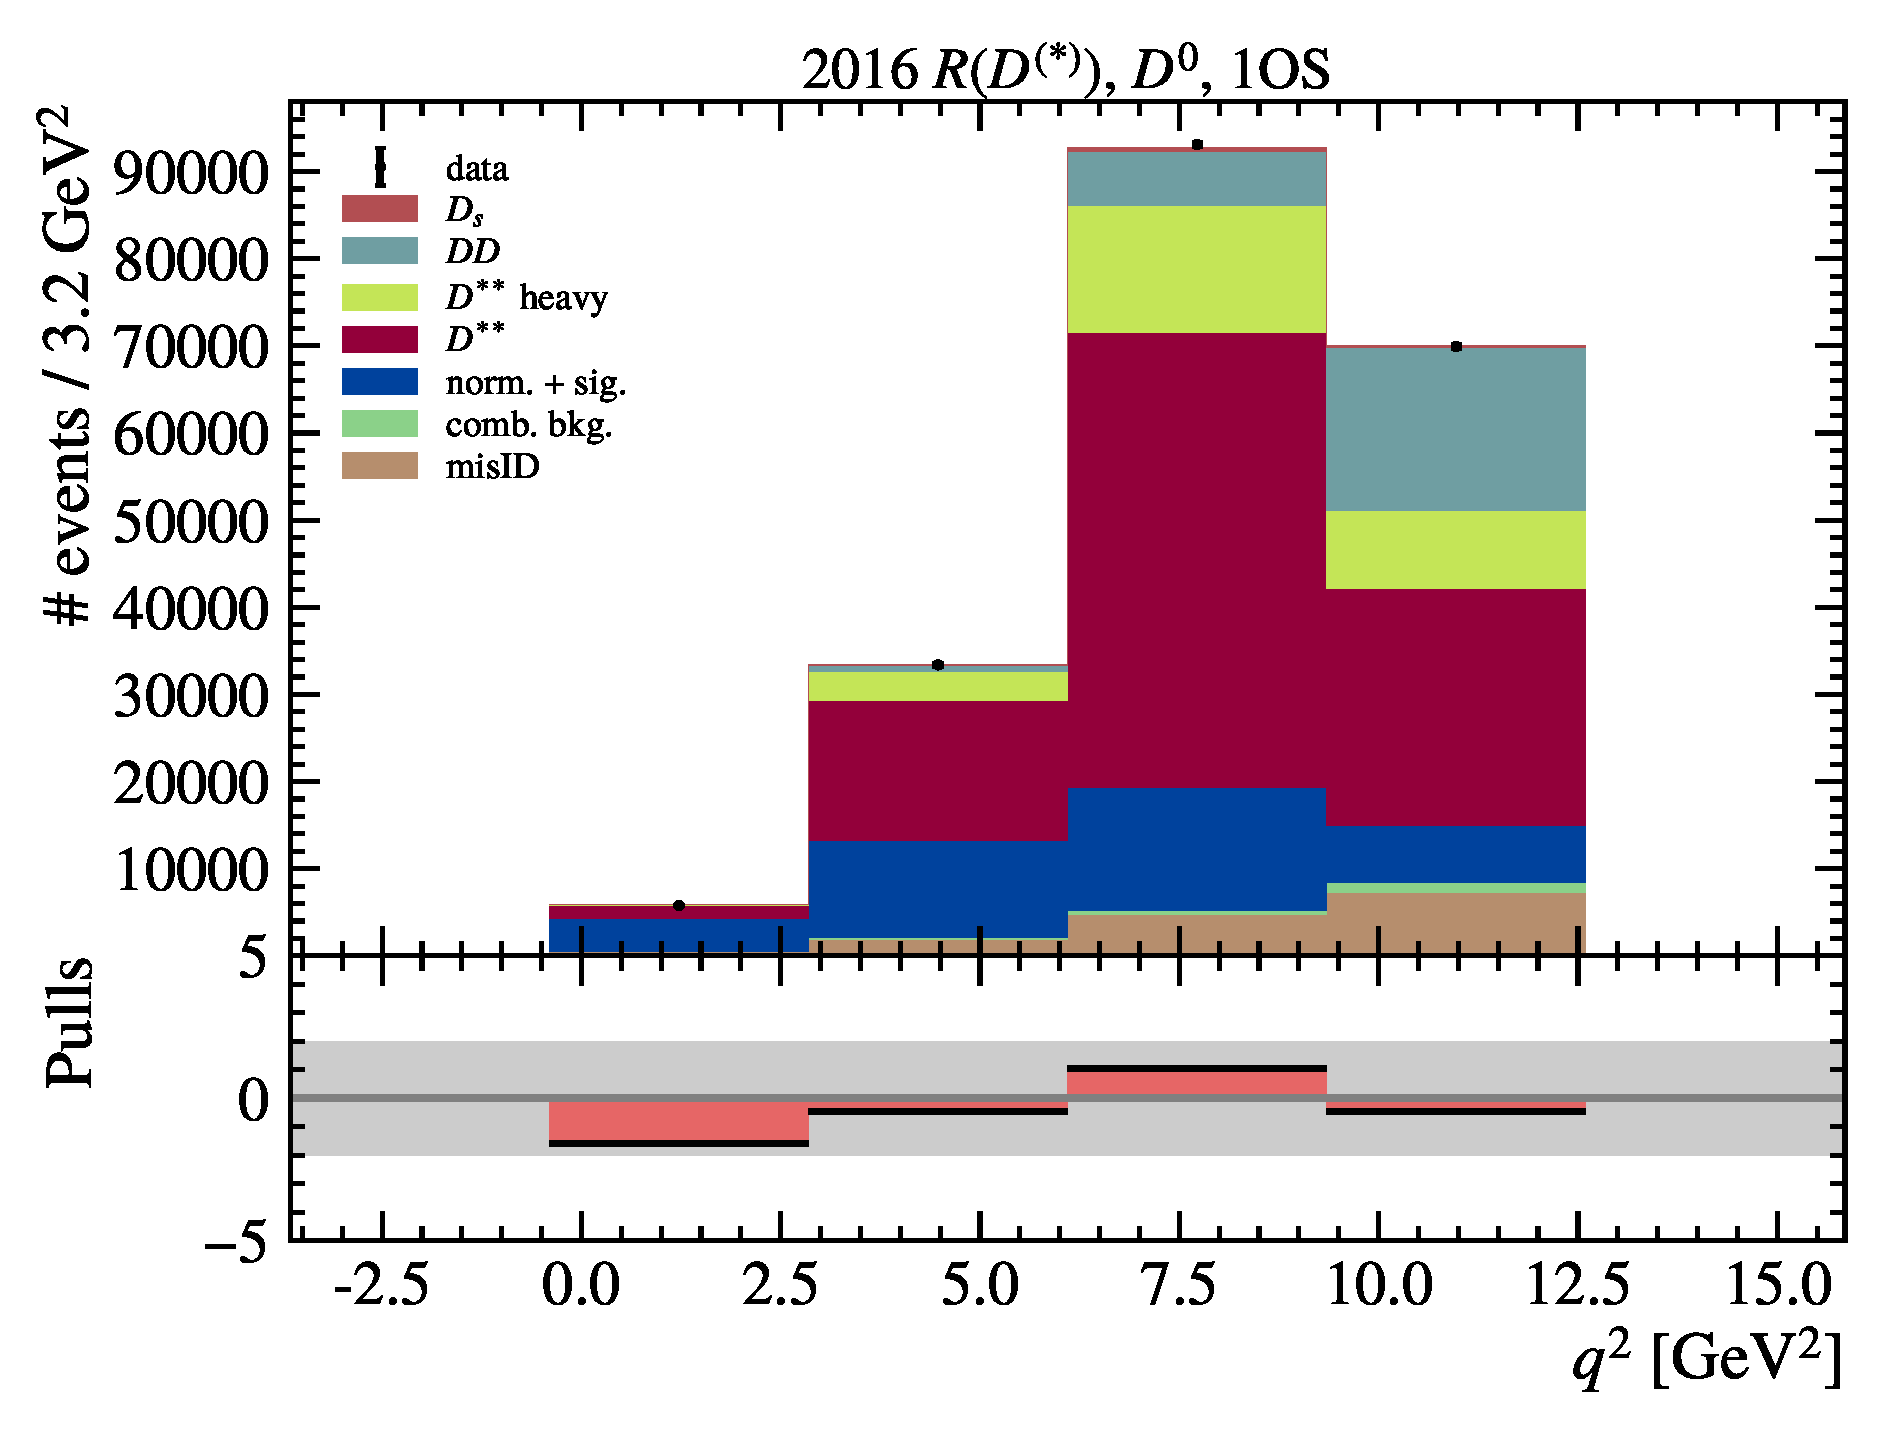
\includegraphics[width=0.32\textwidth]{./figs-supplemental-plots/init-fit/ctrl/fit_result-stacked-D0-1os-q2.pdf}
        \caption{1OS}
    \end{subfigure}

    \begin{subfigure}{\textwidth}
        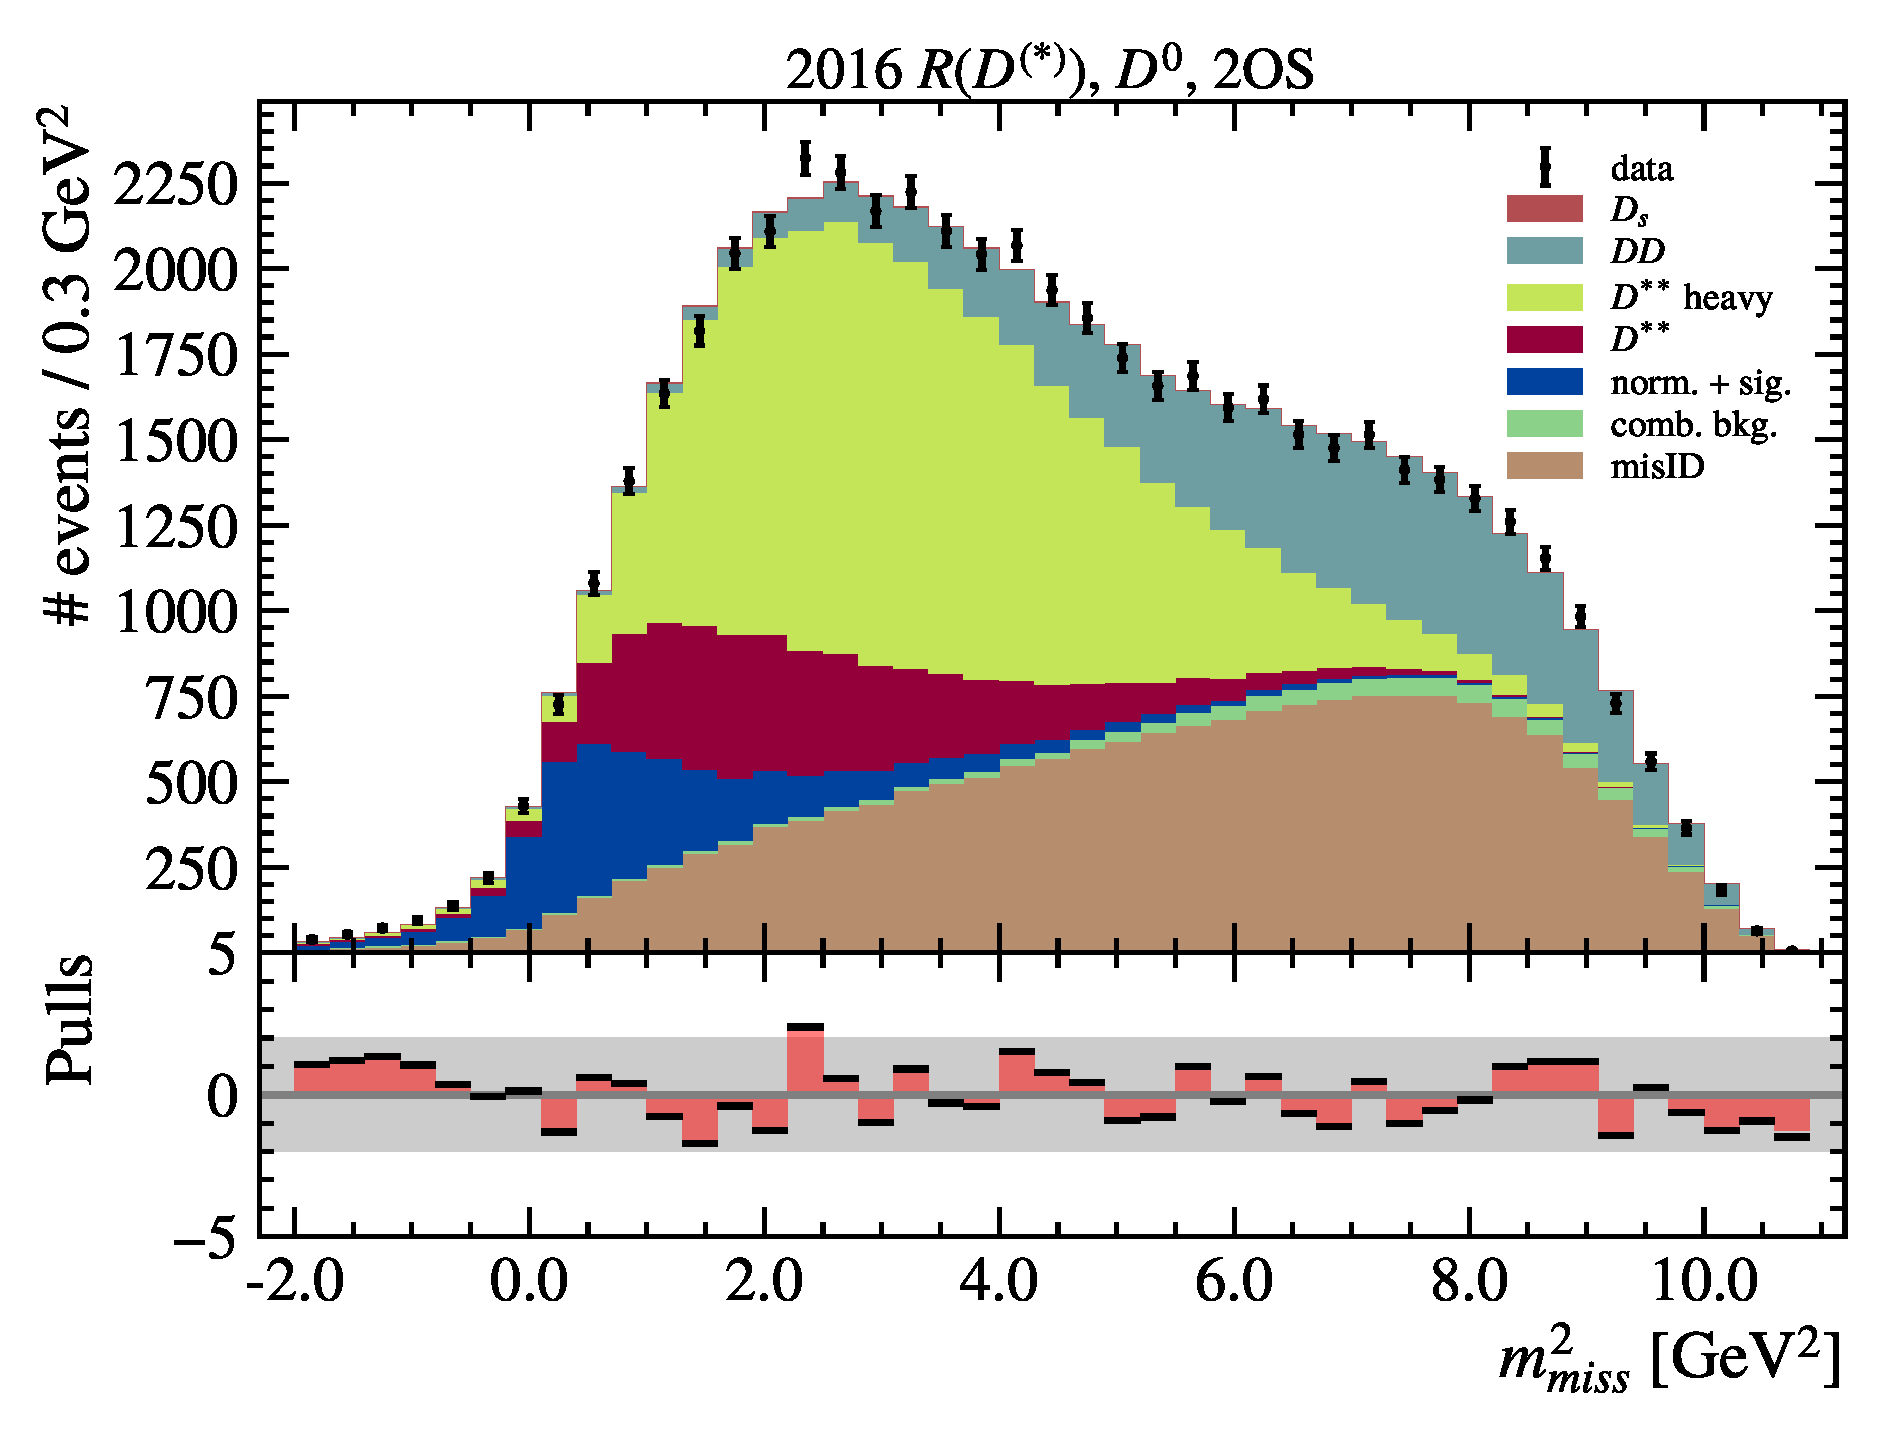
\includegraphics[width=0.32\textwidth]{./figs-supplemental-plots/init-fit/ctrl/fit_result-stacked-D0-2os-mmiss2.pdf}
        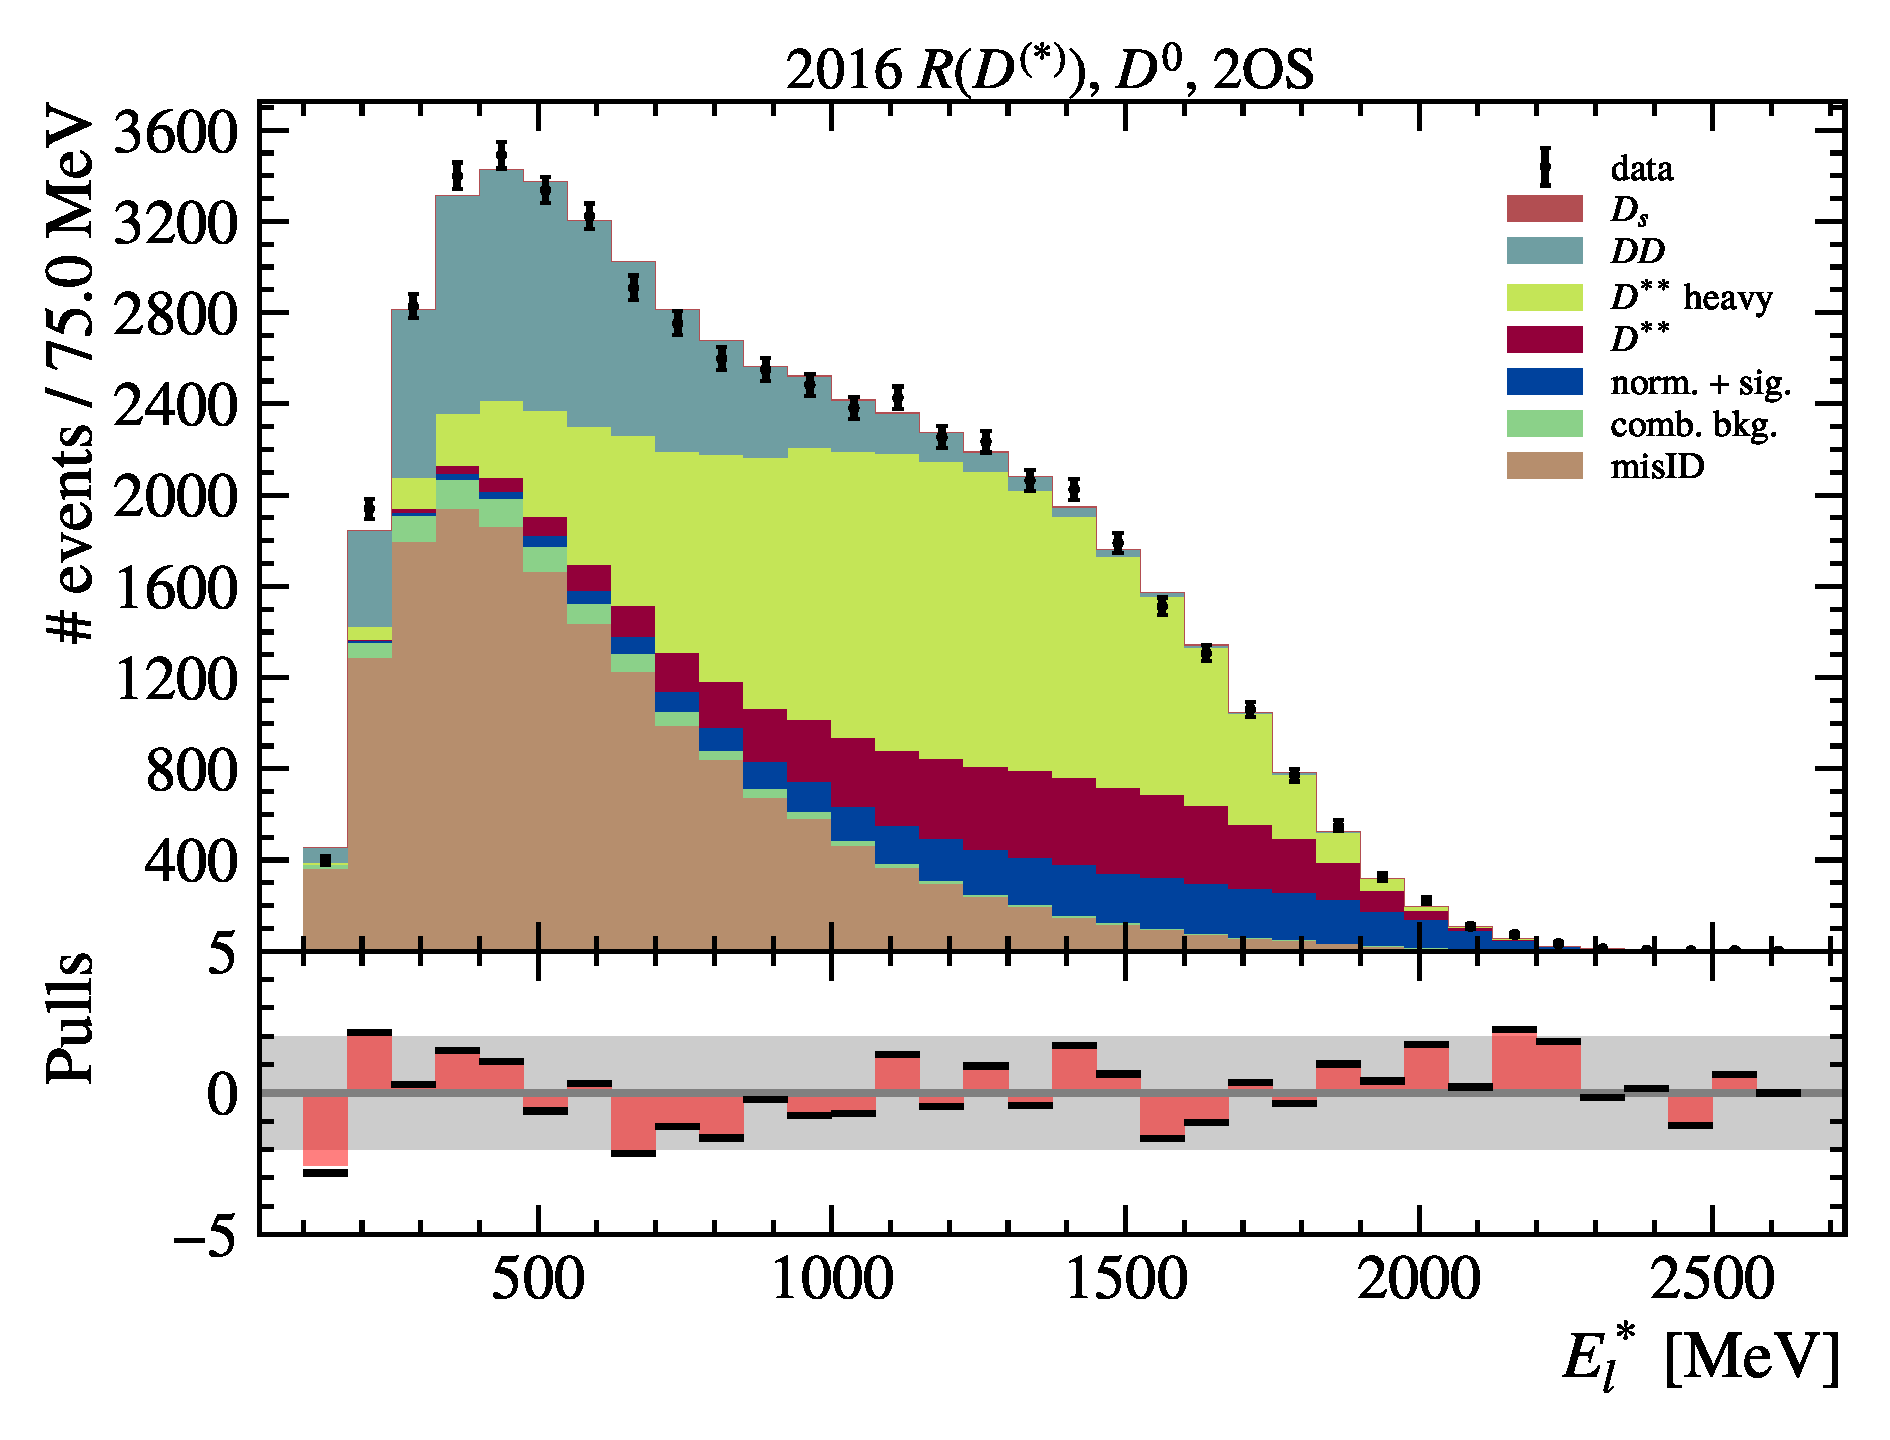
\includegraphics[width=0.32\textwidth]{./figs-supplemental-plots/init-fit/ctrl/fit_result-stacked-D0-2os-el.pdf}
        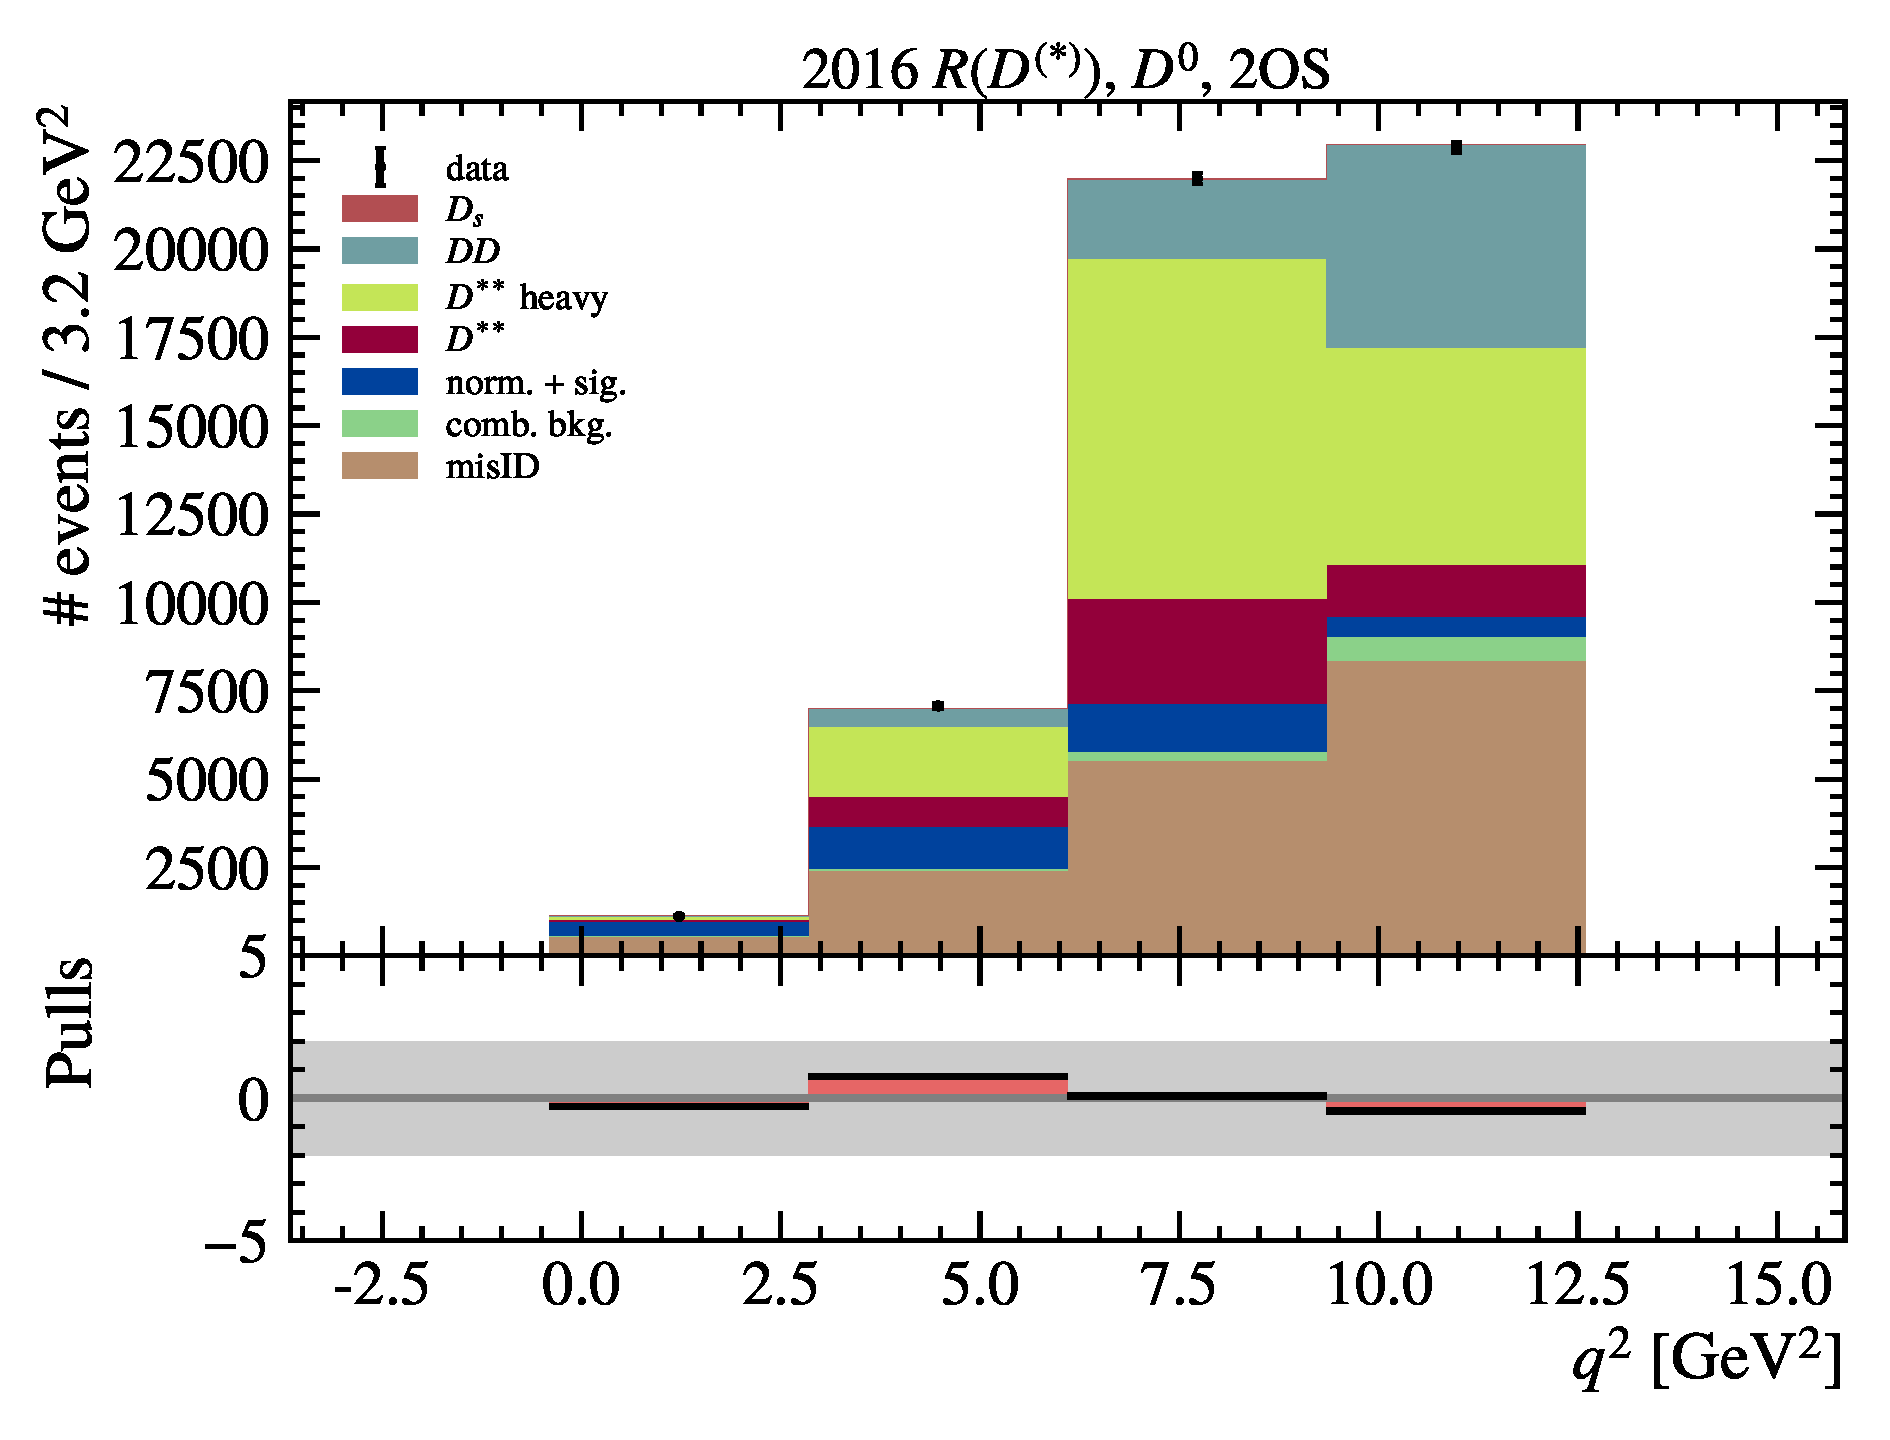
\includegraphics[width=0.32\textwidth]{./figs-supplemental-plots/init-fit/ctrl/fit_result-stacked-D0-2os-q2.pdf}
        \caption{2OS}
    \end{subfigure}

    \begin{subfigure}{\textwidth}
        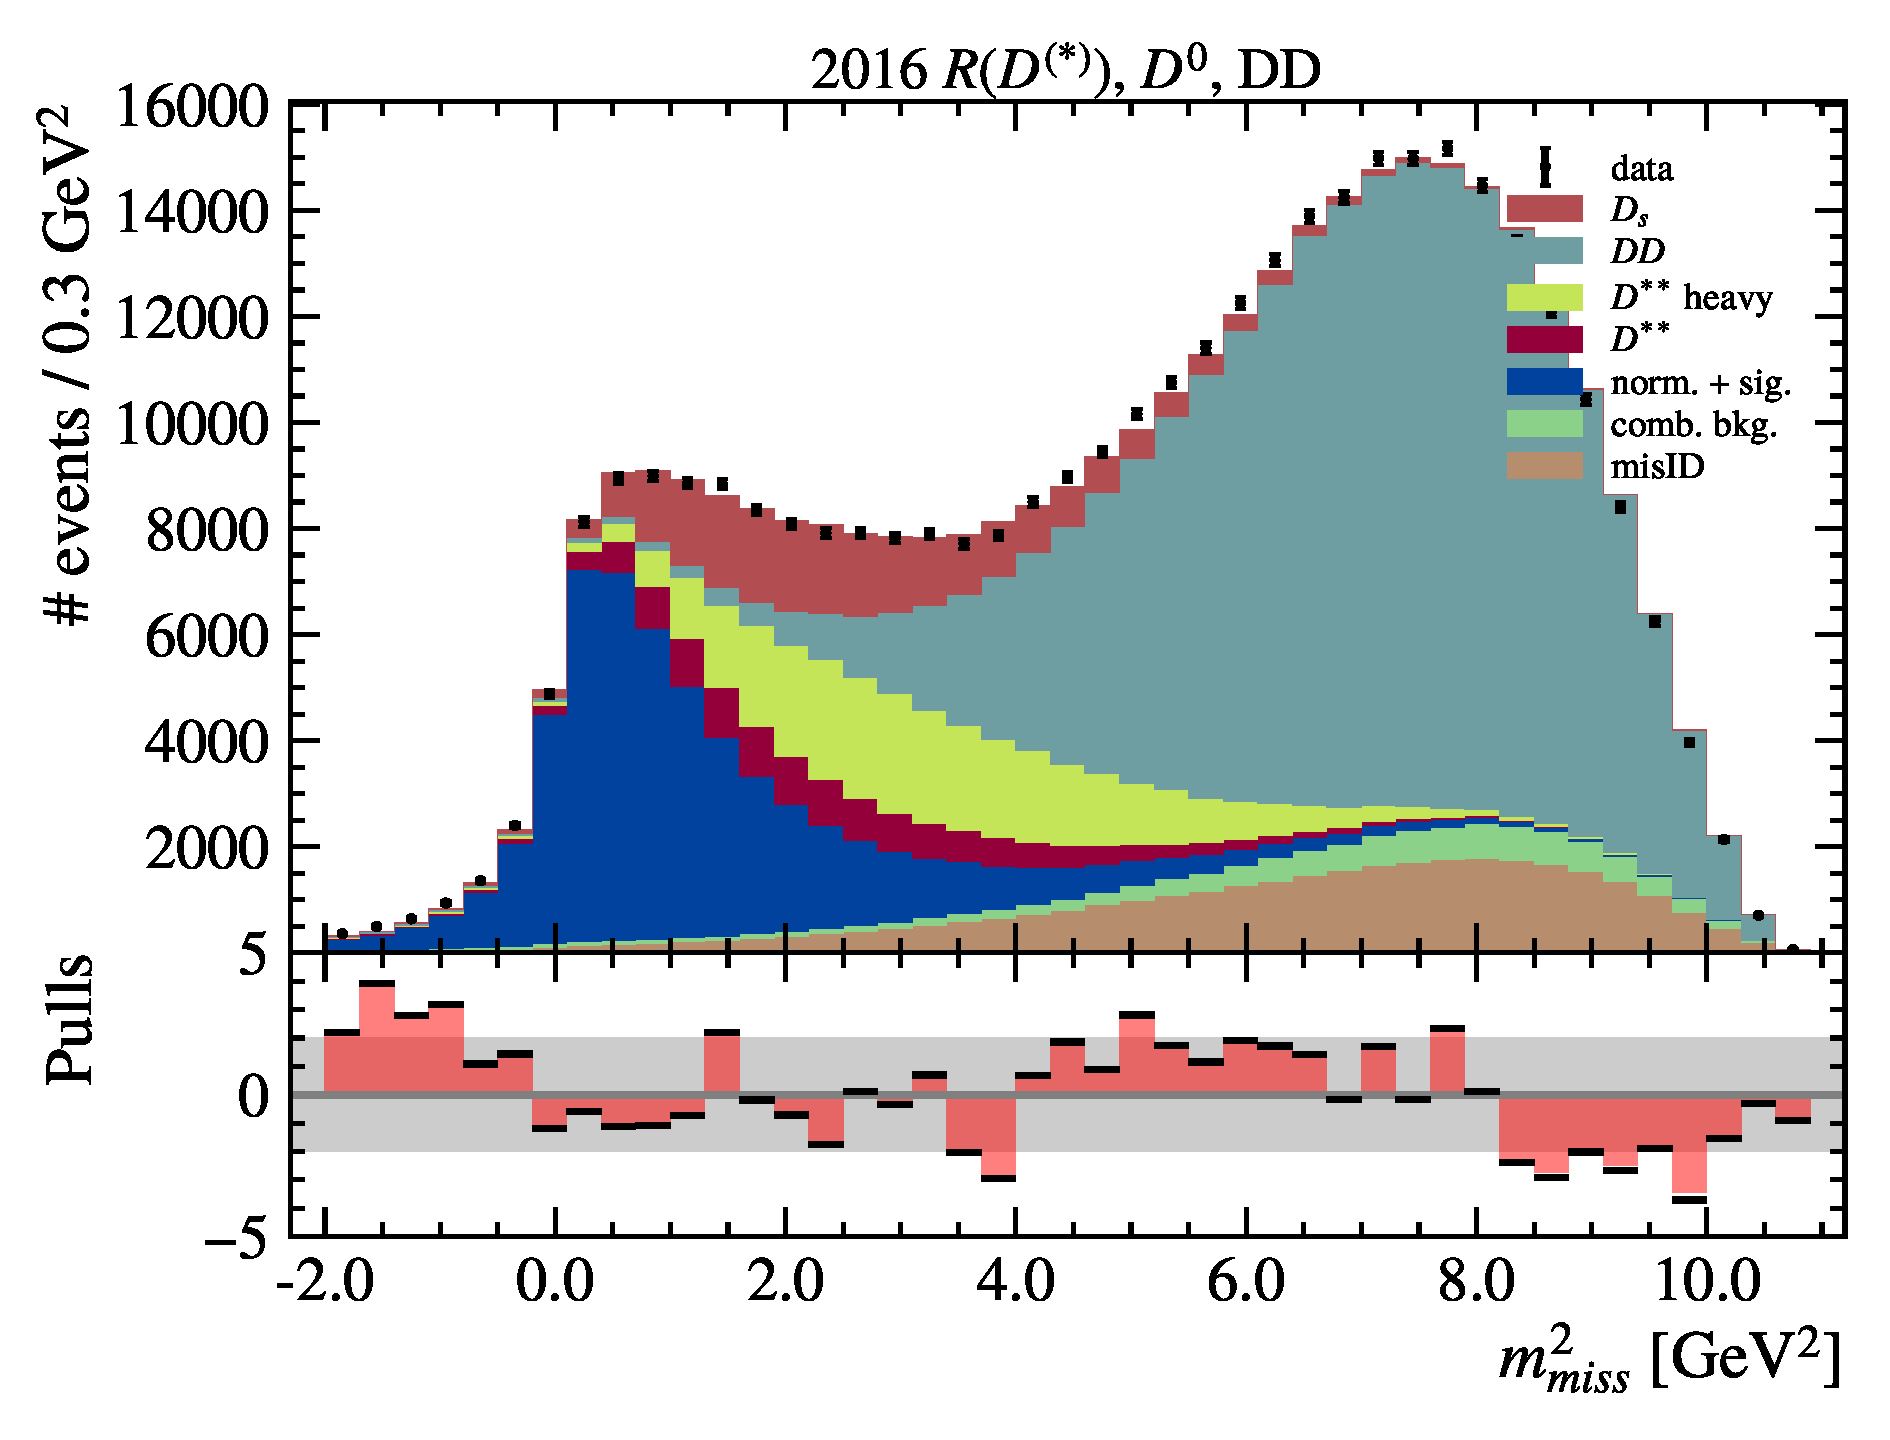
\includegraphics[width=0.32\textwidth]{./figs-supplemental-plots/init-fit/ctrl/fit_result-stacked-D0-dd-mmiss2.pdf}
        \includegraphics[width=0.32\textwidth]{./figs-supplemental-plots/init-fit/ctrl/fit_result-stacked-D0-dd-el.pdf}
        \includegraphics[width=0.32\textwidth]{./figs-supplemental-plots/init-fit/ctrl/fit_result-stacked-D0-dd-q2.pdf}
        \caption{DD}
    \end{subfigure}
    \caption{
        Control fit of \emph{initial fit} in \Dz channel,
        on 1OS, 2OS, and DD samples.
        The Gaussian likelihood penalty on $D^{**}$ form factor uncertainties
        are kept.
    }
    \label{fig:init-fit-ctrl-d0}
\end{figure}

\begin{figure}[htb]
    \centering
    \begin{subfigure}{\textwidth}
        \includegraphics[width=0.32\textwidth]{./figs-supplemental-plots/init-fit/ctrl/fit_result-stacked-Dst-1os-mmiss2.pdf}
        \includegraphics[width=0.32\textwidth]{./figs-supplemental-plots/init-fit/ctrl/fit_result-stacked-Dst-1os-el.pdf}
        \includegraphics[width=0.32\textwidth]{./figs-supplemental-plots/init-fit/ctrl/fit_result-stacked-Dst-1os-q2.pdf}
        \caption{1OS}
    \end{subfigure}

    \begin{subfigure}{\textwidth}
        \includegraphics[width=0.32\textwidth]{./figs-supplemental-plots/init-fit/ctrl/fit_result-stacked-Dst-2os-mmiss2.pdf}
        \includegraphics[width=0.32\textwidth]{./figs-supplemental-plots/init-fit/ctrl/fit_result-stacked-Dst-2os-el.pdf}
        \includegraphics[width=0.32\textwidth]{./figs-supplemental-plots/init-fit/ctrl/fit_result-stacked-Dst-2os-q2.pdf}
        \caption{2OS}
    \end{subfigure}

    \begin{subfigure}{\textwidth}
        \includegraphics[width=0.32\textwidth]{./figs-supplemental-plots/init-fit/ctrl/fit_result-stacked-Dst-dd-mmiss2.pdf}
        \includegraphics[width=0.32\textwidth]{./figs-supplemental-plots/init-fit/ctrl/fit_result-stacked-Dst-dd-el.pdf}
        \includegraphics[width=0.32\textwidth]{./figs-supplemental-plots/init-fit/ctrl/fit_result-stacked-Dst-dd-q2.pdf}
        \caption{DD}
    \end{subfigure}
    \caption{
        Control fit of \emph{initial fit} in \Dstar channel,
        on 1OS, 2OS, and DD samples.
        The Gaussian likelihood penalty on $D^{**}$ form factor uncertainties
        are kept.
    }
    \label{fig:init-fit-ctrl-dst}
\end{figure}

\begin{figure}[htb]
    \centering
    \includegraphics[width=0.32\textwidth]{./figs-supplemental-plots/init-fit/sig/fit_result-stacked-D0-iso-mmiss2.pdf}
    \includegraphics[width=0.32\textwidth]{./figs-supplemental-plots/init-fit/sig/fit_result-stacked-D0-iso-el.pdf}
    \includegraphics[width=0.32\textwidth]{./figs-supplemental-plots/init-fit/sig/fit_result-stacked-D0-iso-q2.pdf}

    \caption{
        Signal fit of \emph{initial fit} in \Dz channel on ISO samples.
    }
    \label{fig:init-fit-sig-d0}
\end{figure}

\begin{figure}[htb]
    \centering
    \includegraphics[width=0.32\textwidth]{./figs-supplemental-plots/init-fit/sig/fit_result-stacked-Dst-iso-mmiss2.pdf}
    \includegraphics[width=0.32\textwidth]{./figs-supplemental-plots/init-fit/sig/fit_result-stacked-Dst-iso-el.pdf}
    \includegraphics[width=0.32\textwidth]{./figs-supplemental-plots/init-fit/sig/fit_result-stacked-Dst-iso-q2.pdf}

    \caption{
        Signal fit of \emph{initial fit} in \Dstar channel on ISO samples.
    }
    \label{fig:init-fit-sig-dst}
\end{figure}


\section{Pre-control fit result}
\label{appx:suppl:fit-pre-ctrl}

The pre-control fit results are listed in
\cref{fig:pre-ctrl-1os-d0,fig:pre-ctrl-2os-d0,fig:pre-ctrl-dd-d0} for the \Dz
channel;
\cref{fig:pre-ctrl-1os-dst,fig:pre-ctrl-2os-dst,fig:pre-ctrl-dd-dst} for the
\Dstar channel.

\begin{figure}[htb]
    \centering
    \includegraphics[width=0.32\textwidth]{./figs-supplemental-plots/pre-ctrl-fit/stacked/fit_result-stacked-D0-1os-mmiss2.pdf}
    \includegraphics[width=0.32\textwidth]{./figs-supplemental-plots/pre-ctrl-fit/stacked/fit_result-stacked-D0-1os-el.pdf}
    \includegraphics[width=0.32\textwidth]{./figs-supplemental-plots/pre-ctrl-fit/stacked/fit_result-stacked-D0-1os-q2.pdf}

    \includegraphics[width=0.24\textwidth]{./figs-supplemental-plots/pre-ctrl-fit/lines_q2_slices/fit_result-lines_q2_idx1-D0-1os-mmiss2.pdf}
    \includegraphics[width=0.24\textwidth]{./figs-supplemental-plots/pre-ctrl-fit/lines_q2_slices/fit_result-lines_q2_idx2-D0-1os-mmiss2.pdf}
    \includegraphics[width=0.24\textwidth]{./figs-supplemental-plots/pre-ctrl-fit/lines_q2_slices/fit_result-lines_q2_idx3-D0-1os-mmiss2.pdf}
    \includegraphics[width=0.24\textwidth]{./figs-supplemental-plots/pre-ctrl-fit/lines_q2_slices/fit_result-lines_q2_idx4-D0-1os-mmiss2.pdf}

    \includegraphics[width=0.24\textwidth]{./figs-supplemental-plots/pre-ctrl-fit/lines_q2_slices/fit_result-lines_q2_idx1-D0-1os-el.pdf}
    \includegraphics[width=0.24\textwidth]{./figs-supplemental-plots/pre-ctrl-fit/lines_q2_slices/fit_result-lines_q2_idx2-D0-1os-el.pdf}
    \includegraphics[width=0.24\textwidth]{./figs-supplemental-plots/pre-ctrl-fit/lines_q2_slices/fit_result-lines_q2_idx3-D0-1os-el.pdf}
    \includegraphics[width=0.24\textwidth]{./figs-supplemental-plots/pre-ctrl-fit/lines_q2_slices/fit_result-lines_q2_idx4-D0-1os-el.pdf}

    \caption{Pre-control fit for 1OS sample, \Dz channel.}
    \label{fig:pre-ctrl-1os-d0}
\end{figure}

\begin{figure}[htb]
    \centering
    \includegraphics[width=0.32\textwidth]{./figs-supplemental-plots/pre-ctrl-fit/stacked/fit_result-stacked-D0-2os-mmiss2.pdf}
    \includegraphics[width=0.32\textwidth]{./figs-supplemental-plots/pre-ctrl-fit/stacked/fit_result-stacked-D0-2os-el.pdf}
    \includegraphics[width=0.32\textwidth]{./figs-supplemental-plots/pre-ctrl-fit/stacked/fit_result-stacked-D0-2os-q2.pdf}

    \includegraphics[width=0.24\textwidth]{./figs-supplemental-plots/pre-ctrl-fit/lines_q2_slices/fit_result-lines_q2_idx1-D0-2os-mmiss2.pdf}
    \includegraphics[width=0.24\textwidth]{./figs-supplemental-plots/pre-ctrl-fit/lines_q2_slices/fit_result-lines_q2_idx2-D0-2os-mmiss2.pdf}
    \includegraphics[width=0.24\textwidth]{./figs-supplemental-plots/pre-ctrl-fit/lines_q2_slices/fit_result-lines_q2_idx3-D0-2os-mmiss2.pdf}
    \includegraphics[width=0.24\textwidth]{./figs-supplemental-plots/pre-ctrl-fit/lines_q2_slices/fit_result-lines_q2_idx4-D0-2os-mmiss2.pdf}

    \includegraphics[width=0.24\textwidth]{./figs-supplemental-plots/pre-ctrl-fit/lines_q2_slices/fit_result-lines_q2_idx1-D0-2os-el.pdf}
    \includegraphics[width=0.24\textwidth]{./figs-supplemental-plots/pre-ctrl-fit/lines_q2_slices/fit_result-lines_q2_idx2-D0-2os-el.pdf}
    \includegraphics[width=0.24\textwidth]{./figs-supplemental-plots/pre-ctrl-fit/lines_q2_slices/fit_result-lines_q2_idx3-D0-2os-el.pdf}
    \includegraphics[width=0.24\textwidth]{./figs-supplemental-plots/pre-ctrl-fit/lines_q2_slices/fit_result-lines_q2_idx4-D0-2os-el.pdf}

    \caption{Pre-control fit for 2OS sample, \Dz channel.}
    \label{fig:pre-ctrl-2os-d0}
\end{figure}

\begin{figure}[htb]
    \centering
    \includegraphics[width=0.32\textwidth]{./figs-supplemental-plots/pre-ctrl-fit/stacked/fit_result-stacked-D0-dd-mmiss2.pdf}
    \includegraphics[width=0.32\textwidth]{./figs-supplemental-plots/pre-ctrl-fit/stacked/fit_result-stacked-D0-dd-el.pdf}
    \includegraphics[width=0.32\textwidth]{./figs-supplemental-plots/pre-ctrl-fit/stacked/fit_result-stacked-D0-dd-q2.pdf}

    \includegraphics[width=0.24\textwidth]{./figs-supplemental-plots/pre-ctrl-fit/lines_q2_slices/fit_result-lines_q2_idx1-D0-dd-mmiss2.pdf}
    \includegraphics[width=0.24\textwidth]{./figs-supplemental-plots/pre-ctrl-fit/lines_q2_slices/fit_result-lines_q2_idx2-D0-dd-mmiss2.pdf}
    \includegraphics[width=0.24\textwidth]{./figs-supplemental-plots/pre-ctrl-fit/lines_q2_slices/fit_result-lines_q2_idx3-D0-dd-mmiss2.pdf}
    \includegraphics[width=0.24\textwidth]{./figs-supplemental-plots/pre-ctrl-fit/lines_q2_slices/fit_result-lines_q2_idx4-D0-dd-mmiss2.pdf}

    \includegraphics[width=0.24\textwidth]{./figs-supplemental-plots/pre-ctrl-fit/lines_q2_slices/fit_result-lines_q2_idx1-D0-dd-el.pdf}
    \includegraphics[width=0.24\textwidth]{./figs-supplemental-plots/pre-ctrl-fit/lines_q2_slices/fit_result-lines_q2_idx2-D0-dd-el.pdf}
    \includegraphics[width=0.24\textwidth]{./figs-supplemental-plots/pre-ctrl-fit/lines_q2_slices/fit_result-lines_q2_idx3-D0-dd-el.pdf}
    \includegraphics[width=0.24\textwidth]{./figs-supplemental-plots/pre-ctrl-fit/lines_q2_slices/fit_result-lines_q2_idx4-D0-dd-el.pdf}

    \caption{Pre-control fit for DD sample, \Dz channel.}
    \label{fig:pre-ctrl-dd-d0}
\end{figure}

\begin{figure}[htb]
    \centering
    \includegraphics[width=0.32\textwidth]{./figs-supplemental-plots/pre-ctrl-fit/stacked/fit_result-stacked-Dst-1os-mmiss2.pdf}
    \includegraphics[width=0.32\textwidth]{./figs-supplemental-plots/pre-ctrl-fit/stacked/fit_result-stacked-Dst-1os-el.pdf}
    \includegraphics[width=0.32\textwidth]{./figs-supplemental-plots/pre-ctrl-fit/stacked/fit_result-stacked-Dst-1os-q2.pdf}

    \includegraphics[width=0.24\textwidth]{./figs-supplemental-plots/pre-ctrl-fit/lines_q2_slices/fit_result-lines_q2_idx1-Dst-1os-mmiss2.pdf}
    \includegraphics[width=0.24\textwidth]{./figs-supplemental-plots/pre-ctrl-fit/lines_q2_slices/fit_result-lines_q2_idx2-Dst-1os-mmiss2.pdf}
    \includegraphics[width=0.24\textwidth]{./figs-supplemental-plots/pre-ctrl-fit/lines_q2_slices/fit_result-lines_q2_idx3-Dst-1os-mmiss2.pdf}
    \includegraphics[width=0.24\textwidth]{./figs-supplemental-plots/pre-ctrl-fit/lines_q2_slices/fit_result-lines_q2_idx4-Dst-1os-mmiss2.pdf}

    \includegraphics[width=0.24\textwidth]{./figs-supplemental-plots/pre-ctrl-fit/lines_q2_slices/fit_result-lines_q2_idx1-Dst-1os-el.pdf}
    \includegraphics[width=0.24\textwidth]{./figs-supplemental-plots/pre-ctrl-fit/lines_q2_slices/fit_result-lines_q2_idx2-Dst-1os-el.pdf}
    \includegraphics[width=0.24\textwidth]{./figs-supplemental-plots/pre-ctrl-fit/lines_q2_slices/fit_result-lines_q2_idx3-Dst-1os-el.pdf}
    \includegraphics[width=0.24\textwidth]{./figs-supplemental-plots/pre-ctrl-fit/lines_q2_slices/fit_result-lines_q2_idx4-Dst-1os-el.pdf}

    \caption{Pre-control fit for 1OS sample, \Dstar channel.}
    \label{fig:pre-ctrl-1os-dst}
\end{figure}

\begin{figure}[htb]
    \centering
    \includegraphics[width=0.32\textwidth]{./figs-supplemental-plots/pre-ctrl-fit/stacked/fit_result-stacked-Dst-2os-mmiss2.pdf}
    \includegraphics[width=0.32\textwidth]{./figs-supplemental-plots/pre-ctrl-fit/stacked/fit_result-stacked-Dst-2os-el.pdf}
    \includegraphics[width=0.32\textwidth]{./figs-supplemental-plots/pre-ctrl-fit/stacked/fit_result-stacked-Dst-2os-q2.pdf}

    \includegraphics[width=0.24\textwidth]{./figs-supplemental-plots/pre-ctrl-fit/lines_q2_slices/fit_result-lines_q2_idx1-Dst-2os-mmiss2.pdf}
    \includegraphics[width=0.24\textwidth]{./figs-supplemental-plots/pre-ctrl-fit/lines_q2_slices/fit_result-lines_q2_idx2-Dst-2os-mmiss2.pdf}
    \includegraphics[width=0.24\textwidth]{./figs-supplemental-plots/pre-ctrl-fit/lines_q2_slices/fit_result-lines_q2_idx3-Dst-2os-mmiss2.pdf}
    \includegraphics[width=0.24\textwidth]{./figs-supplemental-plots/pre-ctrl-fit/lines_q2_slices/fit_result-lines_q2_idx4-Dst-2os-mmiss2.pdf}

    \includegraphics[width=0.24\textwidth]{./figs-supplemental-plots/pre-ctrl-fit/lines_q2_slices/fit_result-lines_q2_idx1-Dst-2os-el.pdf}
    \includegraphics[width=0.24\textwidth]{./figs-supplemental-plots/pre-ctrl-fit/lines_q2_slices/fit_result-lines_q2_idx2-Dst-2os-el.pdf}
    \includegraphics[width=0.24\textwidth]{./figs-supplemental-plots/pre-ctrl-fit/lines_q2_slices/fit_result-lines_q2_idx3-Dst-2os-el.pdf}
    \includegraphics[width=0.24\textwidth]{./figs-supplemental-plots/pre-ctrl-fit/lines_q2_slices/fit_result-lines_q2_idx4-Dst-2os-el.pdf}

    \caption{Pre-control fit for 2OS sample, \Dstar channel.}
    \label{fig:pre-ctrl-2os-dst}
\end{figure}

\begin{figure}[htb]
    \centering
    \includegraphics[width=0.32\textwidth]{./figs-supplemental-plots/pre-ctrl-fit/stacked/fit_result-stacked-Dst-dd-mmiss2.pdf}
    \includegraphics[width=0.32\textwidth]{./figs-supplemental-plots/pre-ctrl-fit/stacked/fit_result-stacked-Dst-dd-el.pdf}
    \includegraphics[width=0.32\textwidth]{./figs-supplemental-plots/pre-ctrl-fit/stacked/fit_result-stacked-Dst-dd-q2.pdf}

    \includegraphics[width=0.24\textwidth]{./figs-supplemental-plots/pre-ctrl-fit/lines_q2_slices/fit_result-lines_q2_idx1-Dst-dd-mmiss2.pdf}
    \includegraphics[width=0.24\textwidth]{./figs-supplemental-plots/pre-ctrl-fit/lines_q2_slices/fit_result-lines_q2_idx2-Dst-dd-mmiss2.pdf}
    \includegraphics[width=0.24\textwidth]{./figs-supplemental-plots/pre-ctrl-fit/lines_q2_slices/fit_result-lines_q2_idx3-Dst-dd-mmiss2.pdf}
    \includegraphics[width=0.24\textwidth]{./figs-supplemental-plots/pre-ctrl-fit/lines_q2_slices/fit_result-lines_q2_idx4-Dst-dd-mmiss2.pdf}

    \includegraphics[width=0.24\textwidth]{./figs-supplemental-plots/pre-ctrl-fit/lines_q2_slices/fit_result-lines_q2_idx1-Dst-dd-el.pdf}
    \includegraphics[width=0.24\textwidth]{./figs-supplemental-plots/pre-ctrl-fit/lines_q2_slices/fit_result-lines_q2_idx2-Dst-dd-el.pdf}
    \includegraphics[width=0.24\textwidth]{./figs-supplemental-plots/pre-ctrl-fit/lines_q2_slices/fit_result-lines_q2_idx3-Dst-dd-el.pdf}
    \includegraphics[width=0.24\textwidth]{./figs-supplemental-plots/pre-ctrl-fit/lines_q2_slices/fit_result-lines_q2_idx4-Dst-dd-el.pdf}

    \caption{Pre-control fit for DD sample, \Dstar channel.}
    \label{fig:pre-ctrl-dd-dst}
\end{figure}
